\documentclass[10pt]{article}

\usepackage{stmaryrd, amssymb,amsmath,amsthm,titling,blindtext,cite,opendeduction,epigraph,afterpage}
% mathabx
\usepackage{natbib, setspace, rotating, mathtools, hyperref,rotating,cancel,bussproofs,tikz}
\usetikzlibrary{positioning}
\usepackage[font=small,labelfont=bf]{caption}
\usepackage[a4paper, total={5.5in, 9in}]{geometry}

\usepackage{graphicx}
\graphicspath{ {./images/} }

\bibliographystyle{abbrv}
%\bibliographystyle{ACM-Reference-Format}

\hypersetup{
	colorlinks=true,
	linkcolor=blue,
	filecolor=magenta,      
	urlcolor=blue,
	pdftitle={Overleaf Example},
	pdfpagemode=FullScreen,
}

%% code from mathabx.sty and mathabx.dcl
\DeclareFontFamily{U}{mathx}{\hyphenchar\font45}
\DeclareFontShape{U}{mathx}{m}{n}{
	<5> <6> <7> <8> <9> <10>
	<10.95> <12> <14.4> <17.28> <20.74> <24.88>
	mathx10
}{}
\DeclareSymbolFont{mathx}{U}{mathx}{m}{n}
\DeclareMathAccent{\widecheck}{0}{mathx}{"71}
\DeclareMathAccent{\wideparen}{0}{mathx}{"75}

\def\cs#1{\texttt{\char`\\#1}}

\setlength{\epigraphwidth}{0.6\textwidth}

\newtheorem{theorem}{Theorem}[section]
\newtheorem{corollary}[theorem]{Corollary}
\newtheorem{lemma}[theorem]{Lemma}
\newtheorem{proposition}[theorem]{Proposition}
\newtheorem*{conjecture}{Conjecture}
\theoremstyle{definition}\newtheorem{remark}[theorem]{Remark}
\theoremstyle{definition}\newtheorem{example}[theorem]{Example}
\theoremstyle{definition}\newtheorem{definition}[theorem]{Definition}

\newcommand{\SKSProp}{{\mathsf{SKSg}_{\textbf{\textit{P}}}}}
\newcommand{\SKSq}{{\mathsf{SKSg1}}}
\newcommand{\SKSqDecomp}{{\mathsf{SKS1}}}
\newcommand{\FalsifierCalculus}{{\mathsf{SKSg\varepsilon}}}
\newcommand{\FalsifierCalculusPrime}{{\mathsf{SKSg\varepsilon'}}}

\newcommand{\aiUp}{{\mathsf{ai\mathord\uparrow}}}
\newcommand{\aiDown}{{\mathsf{ai\mathord\downarrow}}}
\newcommand{\acUp}{{\mathsf{ac\mathord\uparrow}}}
\newcommand{\acDown}{{\mathsf{ac\mathord\downarrow}}}
\newcommand{\awUp}{{\mathsf{aw\mathord\uparrow}}}
\newcommand{\awDown}{{\mathsf{aw\mathord\downarrow}}}

\newcommand{\iUp}{{\mathsf{i\mathord\uparrow}}}
\newcommand{\iDown}{{\mathsf{i\mathord\downarrow}}}
\newcommand{\cUp}{{\mathsf{c\mathord\uparrow}}}
\newcommand{\cDown}{{\mathsf{c\mathord\downarrow}}}
\newcommand{\wUp}{{\mathsf{w\mathord\uparrow}}}
\newcommand{\wDown}{{\mathsf{w\mathord\downarrow}}}

\newcommand{\switch}{{\mathsf{s}}}
\newcommand{\medial}{{\mathsf{m}}}

\newcommand{\qcUp}{{\mathsf{qc\mathord\uparrow}}}
\newcommand{\qcDown}{{\mathsf{qc\mathord\downarrow}}}

\newcommand{\rOneUp}{{\mathsf{r1\mathord\uparrow}}}
\newcommand{\rOneDown}{{\mathsf{r1\mathord\downarrow}}}
\newcommand{\rTwoUp}{{\mathsf{r2\mathord\uparrow}}}
\newcommand{\rTwoDown}{{\mathsf{r2\mathord\downarrow}}}
\newcommand{\rThreeUp}{{\mathsf{r3\mathord\uparrow}}}
\newcommand{\rThreeDown}{{\mathsf{r3\mathord\downarrow}}}
\newcommand{\rFourUp}{{\mathsf{r4\mathord\uparrow}}}
\newcommand{\rFourDown}{{\mathsf{r4\mathord\downarrow}}}
\newcommand{\falsifierRule}{{\mathsf{\varepsilon}}}

\newcommand{\eqProp}{=_{\textbf{P}}}
\newcommand{\eqExists}{=_{\exists}}
\newcommand{\eqForall}{=_{\forall}}

\newcommand{\trueUnit}{\mathsf{t}}
\newcommand{\falseUnit}{\mathsf{f}}

\newcommand{\variablesSet}{\mathsf{Var}}
\newcommand{\functionsSet}{\mathsf{Fun}}
\newcommand{\predicatesSet}{\mathsf{Pred}}

\newcommand{\compByInf}[1]{;_{#1}}
\newcommand{\infDerivation}[1]{|_{#1}}
\newcommand{\seqComp}{;}

\newcommand{\trivialForall}{\forall_0}

\title{A Calculus of Falsifiers}

\author{Cameron Allett}

\begin{document}
	\begin{titlepage}
		\begin{center}
			\vspace*{\fill}
			
			{\Huge\textbf{A Calculus of Falsifiers}}
			
			\vspace{1cm}
			
			{\LARGE Cameron Allett
			
			\vspace*{2cm}
			
			A thesis presented for the degree of Doctor of Philosophy
			
			\vspace{1cm}
			
			%\includegraphics[width=0.4\textwidth]{university}
			
			Department of Computer Science\\
			University of Bath\\
			England, UK\\
			
			\vspace{1cm}
			
			April 2026}
			
			\vspace*{\fill}
		\end{center}
	\end{titlepage}
	
	\pagebreak
	
	\begin{center}
		\textbf{Copyright Notice}
		\vspace{1em}
		\noindent
		\\ Attention is drawn to the fact that copyright of this thesis rests with the author and copyright of any previously published materials included may rest with third parties. This thesis has been supplied on condition that anyone who consults it understands that they must not copy it or use material from it except as licenced, permitted by law or with the consent of the author or other copyright owners, as applicable.
	
		\vspace{10em}
		
		\textbf{Declarations}
		\vspace{1em}
		\noindent
		\\ The material presented here for examination for the award of a research degree by research has not been incorporated into a submission for another degree.
		\vspace{1em}
		\noindent
		\\ I am the author of this thesis, and the work described therein was carried out by myself personally.
	\end{center}
	
	\pagebreak
	
	\noindent
	\textbf{Abstract}
	
	\noindent
	\\ The falsifier calculus, a deep-inference proof system
	for first-order predicate logic in the language of Hilbert’s epsilon-calculus, is introduced. It uses a novel inference rule, the falsifier rule, to introduce epsilon-terms into proofs, distinct from the critical axioms of the traditional epsilon-calculus. The falsifier rule is a generalisation of	one of the quantifier-shifts, inference rules for shifting quantifiers inside and outside of formulae. Like the epsilon-calculus and proof systems which include quantifier-shifts, the falsifier calculus admits non-elementarily smaller cut-free proofs of certain classes of first-order theorems than the sequent calculus.
	
	Analogous to the way in which Herbrand’s Theorem decomposes a proof into a first-order and a propositional part, connected by a Herbrand disjunction as an intermediate formula, the falsifier calculus provides a new decomposition theorem for first-order proofs which induces a new notion of intermediate formula in the epsilon-calculus, falsifier disjunctions. It is demonstrated that certain classes of first-order theorems admit non-elementarily smaller falsifier disjunctions than Herbrand disjunctions.
	
	Through these properties, the falsifier calculus contributes new insights to our understanding of the structure and complexity of proofs in first-order predicate logic. The phenomenon of the non-elementary compression of cut-free proofs has long been of interest in structural proof theory, and the falsifier calculus provides a new perspective on what properties make a proof system admit this compression as well as the role of epsilon-terms in this compression. Furthermore, the decomposition theorem admitted by the falsifier calculus provides a novel perspective on the structure of Herbrand disjunctions and their complexity, yielding new insights into one of the fundamental theorems of classical proof theory.
	
	\pagebreak
	
	\noindent
	\textbf{Acknowledgements}
	
	\noindent
	\\ There are many people who deserve thanks and acknowledgement for their roles in my research and life over the past four years.
	
	My supervisor, Willem Heijltjes, has been an invaluable source of guidance and support throughout my graduate studies and I am deeply grateful for his efforts in helping me to produce the best thesis of which I was capable.
	
	I would like to thank my examiners, Georg Moser and Thomas Powell, for their enthusiasm in engaging with my research and for a stimulating and surprisingly enjoyable viva experience, which itself was the source of several interesting ideas for taking this work forward.
	
 	I am grateful to everyone in the MathFound group in Bath for introducing me to the world of science and for providing an intellectually vibrant setting in which to conduct research. My fellow PhD students – Chris, Torie, Georgi, Hollie, Dan, Keji and Alex – have been a continual source of support, inspiration and interesting discussions and I am lucky to have met such talented people. I am glad to have many memories to look back on my time in Bath fondly.
	
	I would also like to acknowledge everyone in my personal life for watching over me at the most stressful times and for their boundless support and encouragement. My time outside of research has been filled with many enjoyable sea swims, fun visits and adventures around the UK and, of course, an unforgettable Italy trip, which have all been integral to my sanity and wellbeing over this endeavour. I would also like to thank my housemates in T3 for helping me to settle in over my first year in Bath.
	
	% I have also benefitted from and enjoyed discussions with Anupam Das, Sonia Marin, Lutz Strassburger
	
	\pagebreak

	\tableofcontents
	
	\pagebreak
	
	\listoffigures
	
	\pagebreak
	
	\section{Introduction}\label{Introduction}
	
	\epigraph{The relation of the sign to the thing signified is being destroyed, the game of exchanges between signs is being multiplied of itself and for itself. And the increasing complication demands that there should be signs for signs...}{\textit{S. Weil}}
	
	\noindent
	There is a long history of investigating the shape and structure of mathematical proofs. Since the inception of proof theory in the early twentieth century, a range of techniques have been developed to represent and manipulate formal proofs. While early investigations in proof theory were concerned primarily with establishing the completeness and consistency of formal proof systems for various logics, research has tended towards investigations into the complexity and normalisation theory of proofs as the field has matured. This thesis will contribute towards these efforts by providing a new normalisation result for proofs in first-order predicate logic and a new perspective on an old problem in the study of proof complexity: the compression of first-order proofs.
	
	This thesis will introduce a new proof system for first-order predicate logic, called the \textit{falsifier calculus}, and explore its proof-theoretic properties. The falsifier calculus is defined in the language of Hilbert's \textit{epsilon-calculus} \cite{HilbertFoundations}, which extends the language of first-order predicate logic by \textit{$\varepsilon$-terms} $\varepsilon_x A(x)$ for all variables $x$ and formulae $A(x)$ such that, for a given semantics $\llbracket - \rrbracket_{\mathbb{D}}$ with domain $\mathbb{D}$, each $\varepsilon$-term $\varepsilon_x A(x)$ is assigned an element in $\mathbb{D}$ by
	\begin{gather*}
		\llbracket \varepsilon_x A(x) \rrbracket_{\mathbb{D}} = \begin{cases}
			d & \text{if there exists some $d \in \mathbb{D}$ such that $\llbracket A(d) \rrbracket_\mathbb{D}$} \\
			a & \text{for some arbitrary $a \in \mathbb{D}$, otherwise}
		\end{cases}
	\end{gather*}
	where $d$ is chosen by a choice function on $\mathcal{P}(\mathbb{D})$ and $a \in \mathbb{D}$ is fixed. The falsifier calculus uses a novel inference rule for introducing $\varepsilon$-terms into proofs, called the \textit{falsifier rule $\falsifierRule$}, which is given by
	\[
		\drv[] {
			\forall x (A(x) \lor B(x)) ; [\falsifierRule]- ; \forall x A(x) \lor B(\varepsilon_y \overline{A}(y))
		}
	\]
	and is distinct from the critical axioms used to introduce $\varepsilon$-terms into proofs in the traditional epsilon-calculus. Through the use of this rule, the falsifier calculus admits cut-free proofs of certain classes of first-order theorems which are non-elementarily smaller than their corresponding smallest cut-free proofs in traditional proof systems such as the sequent calculus. This compression is also admitted by several other proof systems \cite{BaazUnsoundInferences, BaazLolicEpsilonShorterProofs} so that the falsifier calculus provides a novel insight into the properties that make a proof system admit this compression as well as the role of $\varepsilon$-terms in this compression. Furthermore, the falsifier calculus admits a new decomposition theorem for proofs in first-order predicate logic, the \textit{Falsifier Decomposition Theorem}, providing a new perspective on their structure. The Falsifier Decomposition Theorem can be understood as an analogue to Herbrand's Theorem in which $\varepsilon$-terms may also occur in the upper propositional segment of the proof, resulting in a non-elementary compression over proofs in Herbrand normal form. The Falsifier Decomposition Theorem induces the notion of \textit{falsifier disjunctions}, which are analogues to Herbrand disjunctions in the language of the epsilon-calculus such that certain classes of first-order theorems admit non-elementarily smaller falsifier disjunctions than Herbrand disjunctions, yielding a new perspective on the structure of Herbrand disjunctions and their complexity.
	
	The falsifier calculus is defined using a proof formalism that admits \textit{deep inference}, which allows for greater freedom in applying inference rules than conventional proof systems by allowing them to apply at arbitrary depth inside of formulae. This yields a rich normalisation theory which is not observable in traditional proof formalisms, and which will be exploited in this thesis to prove normalisation results for first-order predicate logic using the falsifier calculus.
	
	\subsection{Proof Theory}
	
	The field of proof theory is generally considered to have been initiated with the introduction of Hilbert's program in the 1920s. The discovery of several apparent paradoxes in foundational areas of mathematics in the late nineteenth and early twentieth centuries had led to a ``foundational crisis of mathematics", to which Hilbert proposed a research program towards resolving. Hilbert's program sought to provide a formal axiomatic foundation for all areas of mathematics and demonstrate the consistency of these axioms, i.e., that they were free of contradiction. With this came the introduction of the first formal deductive systems in mathematics, such as \textit{Hilbert-Frege systems} \cite{CookReckhowFregeSystems}, which are comprised of a list of formula axioms and the inference rule of \textit{modus ponens}, the principle that the formula $B$ may be deduced from the formulae $A$ and $A \rightarrow B$, which is used to derive valid formulae from the axioms. Hilbert's program is usually understood to have come to an end with the publication of Gödel's second incompleteness theorem in 1931 \cite{GodelIncompletenessTheorems}, which demonstrated that any deductive system strong enough to prove the axioms of Peano arithmetic is unable to prove its own consistency.
	
	Although Hilbert-Frege systems and initial investigations in proof theory were able to provide complete proof systems for logics foundational to mathematics such as propositional classical logic and first-order predicate logic, the underlying deductive systems were unwieldy and admitted a proof structure which was far removed from the structure of actual mathematical reasoning. In 1935, Gentzen \cite{GentzenInvestigations} introduced the proof systems of the \textit{sequent calculus} and \textit{natural deduction} for propositional and first-order classical and intuitionistic logic, which were designed so that their inference rules more closely reflected the structure of reasoning in proofs as developed in mathematical practice. As a consequence of this design, the new proof systems were able to express normal forms for proofs which were not observable in Hilbert-Frege systems, providing a better setting in which to systematically investigate the normalisation theory of proofs. The sequent calculus expresses logical judgements in the form of \textit{sequents}
	\[
		A_1, \dots, A_n \vdash B_1, \dots, B_m
	\]
	where $A_1, \dots, A_n, B_1, \dots, B_m$ are formulae, which express that if every $A_i$ is true for $i \in \{1, \dots, n\}$ then at least one $B_j$ is true for $j \in \{1, \dots, m\}$ (i.e., $\overline{A_1} \lor \dots \lor \overline{A_n} \lor B_1 \lor \dots \lor B_m$ is a valid formula). Proofs in the sequent calculus are comprised of inference rules which contain a non-negative integer number of sequent premises and a single sequent conclusion. Inference rules are composed to form proofs so that the resultant sequent-calculus proofs exhibit a tree-like structure, with inference rules as vertices and formulae as edges.
	
	Gentzen proved a fundamental normalisation result for the sequent calculus in the form of the \textit{Hauptsatz}, or cut-elimination theorem, which states that the cut rule, which is given in the sequent calculus by
	\begin{prooftree}
		\def\fCenter{\mbox{\ $\vdash$\ }}
		\AxiomC{$\Gamma \vdash \Delta, A$}
		\AxiomC{$A, \Sigma \vdash \Pi$}
		\RightLabel{Cut}
		\BinaryInf$\Gamma , \Sigma \fCenter \Delta, \Pi$
	\end{prooftree}
	where $\Gamma, \Delta, \Sigma$ and $\Pi$ are sequences of formulae and $A$ is a formula, is eliminable from sequent-calculus proofs. Observe that the cut rule may be understood as being equivalent to modus ponens due to the classical logical equivalence $A \rightarrow B \equiv \overline{A} \lor B$. The cut rule is the only inference rule in the sequent calculus which is not \textit{analytic}, meaning it is the only inference rule which may contain symbols in its premise which are not contained in its conclusion. Consequently, cut-free proofs in the sequent calculus admit the \textit{subformula property}: the property that every formula which occurs in the proof is a subformula of the conclusion of the proof. Consistency of the sequent calculus is an immediate corollary of the subformula property, since it follows that a cut-free proof of the false unit would necessarily assume the false unit as a premise. Gentzen would also later employ the cut-elimination theorem to provide the first proof of the consistency of Peano arithmetic relative to the axioms of ZFC set theory \cite{GentzenConsistencyProof}.
	
	Natural deduction is a restriction of the sequent calculus so that judgements are of the form
	\[
		A_1, \dots, A_n \vdash B
	\]
	where $A_1, \dots, A_n$ and $B$ are formulae. Prawitz \cite{PrawitzNaturalDeduction} would later extend the \textit{Hauptsatz} and other normalisation results of the sequent calculus to natural deduction in 1965. The sequent calculus and natural deduction have provided the setting in which most contemporary research in proof theory is conducted. Several adaptations of these formalisms have been developed in order to demonstrate cut elimination for various logics which do not admit cut elimination in the standard sequent calculus, such as \textit{labelled sequent calculi} \cite{AlwenLabelledBBI}, \textit{hypersequent calculi} \cite{AvronHypersequents, BaazCiabattaHypersequentsForGodel} and \textit{nested sequent calculi} \cite{KaiNestedSequents}.
	
	This thesis explores the proof theory of \textit{deep inference} \cite{AlessioSystemOfInteractionAndStructure}, which is a relatively new design methodology for proof formalisms which breaks from the conventions of Gentzen proof theory by allowing inference rules to apply at arbitrary depth inside of formulae. The greater freedom in applying inference rules in deep-inference formalisms enables the expression of new normal forms for proofs which are not observable in Gentzen systems as well as for speedups over conventional proof systems. The central proof system of this thesis, the falsifier calculus, is defined in the deep-inference formalism of \textit{open deduction} \cite{GuglielmiGundersenParigotOpenDeduction} and exploits the properties of deep-inference proof theory to provide novel insights into the complexity and normalisation theory of proofs in first-order predicate logic. The proof theory and history of deep inference are overviewed in more detail in Subsection \ref{DeepInferenceSection} below.
	
	As the field of proof theory studies mathematical proofs as formal mathematical objects in their own right, it has also seen application in other areas of mathematics as well as the founding of several subfields. Ordinal analysis \cite{RathjenOrdinalAnalysis} is a subfield of proof theory that compares the relative consistency strength of mathematical and arithmetic theories by assigning to each theory a transfinite \textit{proof-theoretic ordinal} that serves as a measure of its relative consistency strength compared to other theories. Reverse mathematics \cite{ReverseMathematicsTextbook} is a subfield of proof theory that examines which axioms are necessary to prove a given mathematical theorem. Proof mining \cite{KohlenbachOlivaProofMiningOverview} applies proof-theoretic techniques to known proofs in other areas of mathematics to extract explicit quantitative information from proofs which otherwise appear to be non-constructive. The study of proof complexity is also a subfield of proof theory in its own right and has deep connections to fundamental problems in complexity theory \cite{CookLengthsOfProofs}. A more recent subfield of proof theory is that of interactive theorem provers (e.g., Lean, Coq, Isabelle, Agda), which are computer programming languages that may be used to formalise mathematical proofs in order to verify their correctness.
	
	This thesis contributes to proof theory in two main ways: by providing a new normalisation result for proofs in first-order predicate logic and a new perspective on the phenomenon of the non-elementary compression of cut-free proofs. The falsifier calculus admits a new decomposition theorem for first-order proofs, Theorem \ref{FalsifierNormalForm} the Falsifier Decomposition Theorem, which is an analogue of Herbrand's Theorem in which $\varepsilon$-terms may appear in the uppermost segment of the proof alongside its propositional content. The Falsifier Decomposition Theorem induces the notion of falsifier disjunctions, which are analogues to Herbrand disjunctions in the language of the epsilon-calculus such that certain classes of first-order theorems admit non-elementarily smaller falsifier disjunctions than Herbrand disjunctions. This yields a novel insight into the structure and complexity of Herbrand disjunctions and first-order proofs more broadly. The fact that certain proof systems admit non-elementarily smaller cut-free proofs than Gentzen's sequent calculus has long been of interest in the study of first-order proof complexity \cite{BaazSkolemization, BaazUnsoundInferences, BaazLolicEpsilonShorterProofs} and the Falsifier Decomposition Theorem provides a new perspective on the properties that make a proof system admit this compression and the role of $\varepsilon$-terms in this compression.
	
	\subsection{Predicate Logic}
	
	In his \textit{Begriffsschrift} \cite{FregeBegriffsschrift}, in an effort to develop a formal language in which to express and reason about arithmetical truths, Frege introduced the first formalisation of first-order predicate logic. Remarkably, the syntax of his predicate logic has seen widespread application and utility in a range of disciplines through to the present day, seeing only stylistic and presentational adaptations since its publication in 1879. The syntax of first-order predicate logic extends the language of propositional classical logic by the universal quantifier $\forall$ and the existential quantifier $\exists$, which are respectively read ``for all" and ``there exists", so that predicate logic allows for the expression of reasoning over elements of a domain. The first completeness proof for first-order predicate logic appeared in Gödel's 1929 thesis \cite{GodelCompleteness} and the first formal semantics were provided by Tarski in 1931 \cite{TarskiConceptOfTruth}.
	
	In this thesis, the epsilon-calculus is employed as an alternative syntax for first-order predicate logic with the motivation of expressing normalisation and complexity results for first-order proofs which are not observable in the standard syntax of predicate logic. Other alternative syntaxes for predicate logic include those which allow for greater expressivity of the dependence relations between quantifiers than the standard syntax, such as Henkin quantification \cite{HenkinInfinitelyLongFormulas} and independence-friendly logic \cite{HintikkaPrinciplesMathematics}, and those which compare the cardinalities of the subsets of the domain which satisfy certain predicates, such as the Härtig quantifier \cite{HerreHartig} and the Frege quantifier \cite{AntonelliFregeQuantifier}. There is growing interest in investigating the proof theory of such syntaxes \cite{BaazHenkin}, placing this work in the broader space of understanding the proof theory of alternative formulations of predicate logic.
	
	\subsection{Herbrand's Theorem}\label{HerbrandSection}
	
	\textit{Herbrand's Theorem} \cite{HerbrandThesis} is one of the central theorems of first-order proof theory. It essentially provides a means of reducing provability in first-order predicate logic to provability in propositional classical logic by means of eliminating the existential quantifiers from a first-order formula. The theorem was first proved in Herbrand's thesis in 1930 for arbitrary first-order formulae, however many statements and restricted forms of the theorem can be found in the literature. Following an overview due to Buss \cite{BussHerbrand, BussIntroductionToProofTheory} (with a correction due to McKinley \cite{McKinleyBussCorrection}), the general version of Herbrand's Theorem for arbitrary formulae in first-order predicate logic in a language which contains a least one constant symbol may be stated as follows.
	\begin{theorem}[Herbrand's Theorem]\label{BussHerbrandStatement}
		A formula $A$ is valid if and only if it admits a \textit{Herbrand proof}, which consists of:
		\begin{itemize}
			\item A \textit{strong $\lor$-expansion} $A_\lor$ of $A$, which is a formula obtained by repeatedly replacing subformulae of the form $\exists x B$ in $A$ with $\exists x B \lor \exists x B$
			
			\item A prenexation $A^*$ of $A_\lor$, which is a formula obtained by renaming quantifiers and bound variables in $A_\lor$ so that no two quantifiers bind the same variable and then using prenex operations to transform the resultant formula into prenex normal form
			
			\item A witnessing substitution $\sigma$ for $A^*$, which is a sequence of terms $t_1, \dots, t_n$ where $\exists x_1, \dots, \exists x_n$ are all of the existential quantifiers in $A^*$, such that $A^*_{qf} [t_1 / x_1] \dots [t_n / x_n]$ is a propositional tautology, where $A^*_{qf}$ is the formula obtained by deleting every existential and universal quantifier in $A^*$ and $B [t / x]$ denotes the formula obtained by replacing every free occurrence of the variable $x$ in the formula $B$ with the term $t$
		\end{itemize}
	\end{theorem}

	Such statements of Herbrand's Theorem are usually proved in the sequent calculus as a corollary of cut elimination. In ``Buss-style" proofs of Herbrand's Theorem, cut rules are first eliminated from a sequent-calculus proof to make the proof amenable to rule permutations. The cut-free proof is then appropriately modified, permuting existential contraction rules and existential witnessing rules down the proof, to yield a propositional proof of the desired propositional tautology. Herbrand's Theorem does not admit a direct statement in the sequent calculus, instead requiring statements in the form of metatheorems involving formulae which are not directly included in any formal proofs, such as the one given above. However, a direct statement and proof of Herbrand's Theorem in a deep-inference formalism has been provided by Brünnler \cite{KaiCutElimination} in the form of a decomposition theorem, which is given as follows.
	\begin{theorem}[Herbrand's Theorem in Deep Inference]\label{DeepInferenceHerbrand}
		Every valid formula $A$ has a proof of the form
		\[
			\drv[] {
				\forall x_1 \dots \forall x_n \, \drv[border=black] {
					; T[\text{Propositional rules (} \SKSProp \text{)}] ; A'
				} ; |[\{\exists\}] ; A'' ; |[\{\rOneDown, \rTwoDown, \rThreeDown, \rFourDown\}] ; A''' ; |[\{\qcDown\}] ; A
			}
		\]
		which is said to be in \textit{Herbrand normal form}, where the formula $\forall x_1 \dots \forall x_n A'$ is called a \textit{Herbrand disjunction for $A$}, the formula $A''$ is in prenex normal form and the relevant inference rules are the \textit{existential witnessing rule $\exists$}, given by
		\[
			\drv[] {
				B(t) ; [\exists]- ; \exists x B(x)
			}
		\]
		where $t$ is free for $x$ in $B(x)$, the \textit{quantifier-shift} rules $\rOneDown, \rTwoDown, \rThreeDown, \rFourDown$, given by
		{\centering
		\begin{tabular} { c c c c }
			& & & \\
			$\hspace{1em}\drv[] {\forall x (B(x) \lor C) ; [\rOneDown]- ; \forall x B(x) \lor C}$ &
			$\drv[] {\forall x (B(x) \land C) ; [\rTwoDown]- ; \forall x B(x) \land C}$ &
			$\drv[] {\exists x (B(x) \lor C) ; [\rThreeDown]- ; \exists x B(x) \lor C}$ &
			$\drv[] {\exists x (B(x) \land C) ; [\rFourDown]- ; \exists x B(x) \land C}\hspace{1em}$ \\
			& & & \\
		\end{tabular}
		\par}
		where $x$ does not occur free in $C$, and the \textit{existential contraction rule $\qcDown$}, given by
		\[
			\drv[] {
				\exists x B \lor \exists x B ; [\qcDown]- ; \exists x B
			}
		\]
	\end{theorem}
	The inference rules used in the statement of this theorem and the proof system $\SKSProp$ for propositional classical logic are defined in Subsection \ref{ProofSystemsSection}. Observe that this resembles the version of Herbrand's Theorem given by Theorem \ref{BussHerbrandStatement} above, in that the decomposed proof of $A$ in Herbrand normal form closely resembles a Herbrand proof of $A$. However, the proof in Herbrand normal form may be expressed directly in a deep-inference formalism, unlike the Herbrand proof of $A$ which requires an ad hoc definition which is not expressed directly in any formalism. Furthermore, the procedure for transforming a first-order deep-inference proof into Herbrand normal form provided by Brünnler does not require all cut rules to be eliminated from the proof, establishing a kind of independence between Herbrand's Theorem and cut elimination which is not observable in the sequent calculus.
	
	Since first-order predicate logic is undecidable and propositional classical logic is decidable, Herbrand's Theorem may be understood to isolate the undecidable content contained in a first-order proof in the existential rules in the lower segments of a proof in Herbrand normal form. In particular, the existential contraction rule $\qcDown$, given by
	\[
		\drv[] {
			\exists x B \lor \exists x B ; [\qcDown]- ; \exists x B
		}
	\]
	may be understood as a case distinction on the witnesses to the two existential quantifiers in the premise of the rule, in that the existential quantifier in the conclusion of the rule is witnessed by one of the witnesses to the two existential quantifiers in the premise of the rule. As such, we may understand the undecidable content of a first-order proof as lying in the case distinctions contained in instances of the existential contraction rule $\qcDown$, which are isolated in the lowermost segment of a proof in Herbrand normal form.
	
	A simple yet elucidating example of Herbrand's Theorem is provided by the ``drinker's paradox", which is the formula $\exists y \forall x (P(x) \lor \overline{P}(y))$ (or, expressed in a logically equivalent form using an implication symbol, $\exists y \forall x (P(y) \rightarrow P(x))$) and expresses that in any pub, there exists a person such that if they are drinking then everyone in the pub is drinking. The drinker's paradox is true by the following logical argument:
	\begin{quotation}
		There are two cases: either (1) everyone in the pub is drinking, $\forall x P(x)$, or (2) there exists a person $y$ in the pub who is not drinking, $\exists y \overline{P}(y)$. In case (1), since everyone in the pub is drinking, we may assign an arbitrary witness to the existential quantifier $\exists y$ in the drinker's paradox to obtain $\exists y \forall x (P(x) \lor \overline{P}(y))$ as desired. In case (2), since there is a person $y$ in the pub who is not drinking, it follows by the principle of explosion that if $y$ is drinking then everyone in the pub is drinking so that we have $\exists y \forall x (P(x) \lor \overline{P}(y))$ as desired.
	\end{quotation}
	A Herbrand disjunction for the formula is $\forall x_1 \forall x_2 [(P(x_1) \lor \overline{P}(c)) \lor (P(x_2) \lor \overline{P}(x_1))]$, which reflects the two cases in this argument in the two disjuncts. The universally quantified variable $x_1$ is used to perform a case distinction on $P(x_1)$, so that the first disjunct $P(x_1) \lor \overline{P}(c)$ represents case (1), that everyone in the pub is drinking ($\forall x_1 P(x_1)$) and the second disjunct $P(x_2) \lor \overline{P}(x_1)$ represents case (2), that there exists a person in the pub who is not drinking ($\exists y \overline{P}(y)$, where the existential quantifier $\exists y$ is witnessed by $x_1$). A deep-inference proof in Herbrand normal form for the formula using this Herbrand disjunction is given by
	\[
		\drv[] {
			\drv[border=black] {
				\forall x_1 \forall x_2 \, \drv[border=black] {
					\drv[border=black] {
						\trueUnit ; [\iDown]- ; P(x_1) \lor \overline{P}(x_1)
					} ; [=]- ; \drv[border=black] {
						\drv[border=black] {
							P(x_1) \lor \drv[border=black] {
								\falseUnit ; [\wDown]- ; \overline{P}(c)
							}
						} \lor \drv[border=black] {
							\drv[border=black] {
								\falseUnit ; [\wDown]- ; P(x_2)
							} \lor \overline{P}(x_1)
						}
					}
				}
			} ; |[\{\exists\}] ; \exists y_1 \forall x_1 \exists y_2 \forall x_2 (P(x_1) \lor \overline{P}(y_1) \lor P(x_2) \lor \overline{P}(y_2)) ; |[\{\rOneDown, \rThreeDown\}] ; \exists y_1 (\forall x_1 P(x_1) \lor \overline{P}(y_1)) \lor \exists y_2 (\forall x_2 P(x_2) \lor \overline{P}(y_2)) ; [\qcDown]- ; \exists y (\forall x P(x) \lor \overline{P}(y))
		}
	\]
	Observe that, as given by Theorem \ref{DeepInferenceHerbrand} above, the upper segment of the proof is a propositional proof of the Herbrand disjunction $\forall x_1 \forall x_2 [(P(x_1) \lor \overline{P}(c)) \lor (P(x_2) \lor \overline{P}(x_1))]$ and is followed by the lower first-order segments of the proof, which contract the two cases contained in the Herbrand disjunction into a single existential quantifier.
	
	In general, there is no recursive bound on the size of a Herbrand disjunction for a first-order formula in terms of the size of the formula \cite{BussHerbrand}. However, as a consequence of the ``Buss-style" procedure for extracting Herbrand disjunctions from sequent-calculus proofs, there is a non-elementary function bounding the size of a Herbrand disjunction for a first-order formula in terms of the size of a given sequent-calculus proof for the formula \cite{BussHerbrand}. This bound is essentially sharp, in that Statman \cite{StatmanLowerBounds} has demonstrated that there is no elementary function bounding the size of a Herbrand disjunction for a first-order formula in terms of the size of a sequent-calculus proof of the formula. This is related to recent work studying the non-elementary compression of cut-free proofs in first-order predicate logic \cite{BaazSkolemization, BaazUnsoundInferences, BaazLolicEpsilonShorterProofs}, which will also be one of the central focuses of this thesis.
	
	Herbrand's Theorem provides the foundation for Miller's \textit{expansion proofs} \cite{MillerExpansionProofs}, which is a graphical proof system for first-order predicate logic in which each witness to an existential quantifier is represented as an edge connecting the existential quantifier to a disjunct in a Herbrand disjunction. Ralph \cite{BenThesis, RalphExpansionProofs} has provided translations between expansion proofs and deep-inference proofs in Herbrand normal form, demonstrating the equivalence of the two systems. Various extensions of the expansion proofs formalism have been developed which introduce cut rules into the formalism and provide a notion of cut elimination for expansion proofs, such as Heijltjes' \textit{proof forestry} \cite{HeijltjesProofForestry, WillemThesis} and an extension of expansion proofs due to Aschieri, Hetzl and Weller \cite{AschieriHetzlWellerExpansionWithCut}. Other examples of proof systems and approaches to first-order proof theory which are based on Herbrand's Theorem include McKinley's \textit{Herbrand nets} \cite{McKinleyHerbrandNets} and a recent game-semantic approach due to Alcolei, Clairambault, Hyland and Winskel \cite{HylandTrueConcurrency}.
	
	The proof system for first-order predicate introduced in this thesis, the falsifier calculus, provides a new decomposition theorem for first-order proofs which may be understood as a non-constructive analogue of Herbrand's Theorem. The new decomposition theorem induces the notion of \textit{falsifier disjunctions}, which are analogues to Herbrand disjunctions in the language of the epsilon-calculus such that certain classes of theorems admit non-elementarily smaller falsifier disjunctions than Herbrand disjunctions. The $\varepsilon$-terms in a falsifier disjunction represent elements which are drawn from the domain non-constructively, resulting in a compression over Herbrand disjunctions, which are comprised only of ground terms so that they represent the content of a first-order proof in a purely constructive manner.
	
	\subsection{The Epsilon-Calculus}
	
	The \textit{epsilon-calculus} \cite{HilbertFoundations, ZachFinitism, ZachThesis} was introduced as part of Hilbert's program in the early twentieth century, which sought to provide a formal foundation for mathematics and establish its consistency, and is one of the oldest proof-theoretic formalisms for predicate logic. The epsilon-calculus extends the language of predicate logic by \textit{$\varepsilon$-terms} $\varepsilon_x A$ for all variables $x$ and formulae $A$ such that, for a given semantics $\llbracket - \rrbracket_{\mathbb{D}}$ with domain $\mathbb{D}$, each $\varepsilon$-term $\varepsilon_x A(x)$ is assigned an element in $\mathbb{D}$ by
	\begin{gather*}
		\llbracket \varepsilon_x A(x) \rrbracket_{\mathbb{D}} = \begin{cases}
			d & \text{if there exists some $d \in \mathbb{D}$ such that $\llbracket A(d) \rrbracket_\mathbb{D}$} \\
			a & \text{for some arbitrary $a \in \mathbb{D}$, otherwise}
		\end{cases}
	\end{gather*}
	where $d$ is chosen by a choice function on $\mathcal{P}(\mathbb{D})$ and $a \in \mathbb{D}$ is fixed. As such, the epsilon-calculus provides a means of incorporating a choice operator into the syntax of predicate logic. In the epsilon-calculus, quantifiers in a proof may be encoded by $\varepsilon$-terms using the logical equivalences $\exists x A(x) \equiv A(\varepsilon_x A(x))$ and $\forall x A(x) \equiv A(\varepsilon_x \overline{A}(x))$ so that all quantifier information in a first-order proof may be expressed within $\varepsilon$-terms.
	
	In the traditional epsilon-calculus as introduced by Hilbert, $\varepsilon$-terms are introduced into a proof by \textit{critical axioms}, which are inferences of the form
	\[
		A(t) \implies A(\varepsilon_x A(x))
	\]
	and, in the presence of the encodings of quantifiers by $\varepsilon$-terms, form a complete proof system for first-order predicate logic when incorporated into a proof system for propositional classical logic \cite{ZachEpsilonSemantics}. The central theorems of the proof theory of the epsilon-calculus are the \textit{epsilon theorems}, which are conservativity results for the epsilon-calculus and provide a means of eliminating $\varepsilon$-terms from proofs. The \textit{first epsilon theorem} and \textit{second epsilon theorem} (see \cite{MoserZachEpsilonCalculusAndHerbrand}) respectively establish the conservativity of extending propositional classical logic and first-order predicate logic by critical axioms. The \textit{extended first epsilon theorem} \cite{BaazEpsilon, MoserZachEpsilonCalculusAndHerbrand} further establishes that for any quantifier-free, epsilon-free formula $A(x_1, \dots, x_n)$ and $\varepsilon$-terms $\varepsilon_{x_1} B_1, \dots, \varepsilon_{x_n} B_n$ which are respectively free for $x_1, \dots, x_n$ in $A(x_1, \dots, x_n)$, if $A(\varepsilon_{x_1} B_1, \dots, \varepsilon_{x_n} B_n)$ is provable in the epsilon-calculus, then there exist epsilon-free terms $t_j^i$ for $i \in \{1, \dots, n\}$, $j \in \{1, \dots, m\}$ such that
	\[
		\bigvee\limits_{i = 1}^{i=n} A(t_1^i, \dots, t_m^i)
	\]
	is a propositional tautology. Herbrand's Theorem for existential formulae is an immediate corollary of this since existential quantifiers may be encoded by $\varepsilon$-terms using the logical equivalence $\exists x A(x) \equiv A(\varepsilon_x A(x))$. These theorems are traditionally proved using a procedure known as \textit{epsilon substitution}, which recursively eliminates critical axioms from a proof. The epsilon theorems and epsilon substitution are usually stated and proved for the equality-free case, though a treatment of the case with equality has recently been provided by Miyamoto and Moser \cite{MiyamotoMoserEpsilonEquality}. Hetzl \cite{HetzlEpsilonTheorems} has also recently provided a novel proof of the epsilon theorems using expansion proofs.
	
	Aside from its historical interest, the epsilon-calculus has seen a renewal of interest in recent years \cite{MiyamotoMoserEpsilonEquality, MoserZachEpsilonCalculusAndHerbrand, BaazEpsilon, BaazLolicEpsilonShorterProofs, AraiEpsilonId1, MintsEpsilonFirstSecond}, in part due to its complexity advantages over traditional proof systems: the sequent-calculus-based epsilon-calculus admits non-elementarily smaller cut-free proofs of certain classes of theorems than traditional sequent-calculus systems for first-order predicate logic \cite{BaazLolicEpsilonShorterProofs}. This is related to the design of a recently introduced sequent-calculus proof system for first-order predicate logic \cite{BaazUnsoundInferences} which admits this non-elementary compression for cut-free proofs over the standard sequent calculus by the use of inference rules which are locally unsound, but which admits a global correctness condition which is inspired by the epsilon-calculus. The methodology for designing global correctness conditions based on the epsilon-calculus for proof systems which include locally unsound rules has also motivated the definition an analytic sequent-calculus proof system for ``reasonable" fragments of Henkin quantification \cite{BaazLolicHenkin}, which do not admit locally sound sequent-calculus proof systems, as well as to demonstrate that an intermediate logic admits Skolemisation if and only if admits a certain class of rules known as \textit{quantifier-shifts}, which will be discussed later in this thesis (see Subsection \ref{QuantifierShiftsSection}) \cite{BaazSkolemisationIntermediateLogics}.
	
	Despite its complexity benefits and interesting proof-theoretic properties, the epsilon-calculus has received little attention from the wider proof theory community, largely due to its unwieldy nature. In particular, the encodings of quantifiers by $\varepsilon$-terms can result in cumbersome encoded formulae in the epsilon-calculus. For instance, borrowing an example from \cite{BaazEpsilon}, the translation of the simple first-order formula $\exists x \exists y \exists z A(x, y, z)$ into the epsilon-calculus is given by
	\begin{align*}
		&A(\varepsilon_xA(x, \varepsilon_yA(x, y, \varepsilon_zA(x, y, z)), \varepsilon_zA(x, \varepsilon_yA(x, y, \varepsilon_zA(x, y, z)), z)), \varepsilon_yA(\varepsilon_xA(x, \\
		&\varepsilon_yA(x, y, \varepsilon_zA(x, y, z)), \varepsilon_zA(x, \varepsilon_yA(x, y, \varepsilon_zA(x, y, z)), z)), y, \varepsilon_zA(\varepsilon_xA(x, \varepsilon_yA(x, y, \\
		&\varepsilon_zA(x, y, z)), \varepsilon_zA(x, \varepsilon_yA(x, y, \varepsilon_zA(x, y, z)), z)), y, z)), \varepsilon_zA(\varepsilon_xA(x, \varepsilon_yA(x, y, \\
		&\varepsilon_zA(x, y, z)), \varepsilon_zA(x, \varepsilon_yA(x, y, \varepsilon_zA(x, y, z)), z)), \varepsilon_yA(\varepsilon_xA(x, \varepsilon_yA(x, y, \varepsilon_zA(x, y, \\
		&z)), \varepsilon_zA(x, \varepsilon_yA(x, y, \varepsilon_zA(x, y, z)), z)), y, \varepsilon_zA(\varepsilon_xA(x, \varepsilon_yA(x, y, \varepsilon_zA(x, y, z)), \\
		&\varepsilon_zA(x, \varepsilon_yA(x, y, \varepsilon_zA(x, y, z)), z))y, z)), z))
	\end{align*}
	Some solutions to this problem have been suggested, such as an alternative syntax for the epsilon-calculus using Skolem functions due to Davis and Fechter \cite{DavisFectherFreeVariable, FechterThesis} and the introduction of \textit{function variable proofs} by Baaz, Leitsch and Lolić \cite{BaazEpsilon}. The epsilon operator is also implicitly contained in some interactive theorem provers, such as in the logic of the ``\textit{Some}" operator in Isabelle and the ``\textit{strong\_indefinite\_description}" operator in Lean.
	
	This thesis contributes to the proof theory of the epsilon-calculus by providing a new proof system for first-order predicate logic in the language of the epsilon-calculus and demonstrating several normalisation and complexity results for this system. One of the aims of this work is to provide a more accessible treatment of the epsilon-calculus, guided by modern motivations of complexity and normalisation in place of the foundational concerns for completeness and consistency when the epsilon-calculus was originally introduced. The system and results in this thesis also do not use the cumbersome encodings of quantifiers by $\varepsilon$-terms described above, circumventing one of the most notorious shortfalls of the traditional epsilon-calculus.
	
	\subsection{Deep Inference}\label{DeepInferenceSection}
	
	\textit{Deep inference} is a design methodology for proof systems which breaks from the conventions of traditional Gentzen proof theory by allowing inference rules to apply at arbitrary depth inside of formulae. This allows for a more flexible composition mechanism for composing proofs and derivations than in traditional proof systems such as the sequent calculus and natural deduction, giving rise to a new proof theory within the more expressive formalism. The freedom to apply inference rules inside formula contexts yields benefits in proof normalisation, such as more freedom in permuting inference rules around a proof and a finer granularity of inference rules than is observable in traditional proof systems, in that inference rules on arbitrary formulae may be decomposed into derivations of smaller inference rules on atomic formulae and quantifiers. This thesis introduces a new deep-inference proof system for first-order predicate logic, the falsifier calculus, and proves several normalisation results for this system, exploiting these properties of deep-inference proof theory in doing so.
	
	%Although deep-inference formalisms were first introduced by Schütte in his textbook on proof theory \cite{SchutteProofTheory}
	The proof theory of deep inference was first investigated when it was employed by Guglielmi to develop a formalism which could express $\mathsf{BV}$ \cite{AlessioSystemOfInteractionAndStructure}, an extension of multiplicative linear logic by a self-adjoint non-commutative binary connective, which is not expressible in the sequent calculus \cite{TiuNeedForDeepInference}. A proliferation of deep-inference proof systems for other more standard logics followed, such as for propositional classical logic \cite{BrunnlerTiuLocalClassical}, first-order predicate logic \cite{BrunnlerGuglielmiFiniteChoice}, linear logic \cite{StrassburgerLocalLinear}, intuitionistic logic \cite{TiuLocalIntuitionistic} and modal logics \cite{StewartStouppaModalLogics}. Early research in deep inference primarily used the deep-inference proof formalism of \textit{the calculus of structures} \cite{AlessioSystemOfInteractionAndStructure}, which represents proofs and derivations as sequences of formulae connected vertically by inference rules which act at arbitrary depth inside formulae, so that a total vertical ordering of inference rules exists for every derivation. Contemporary research generally prefers to use the deep-inference formalism of \textit{open deduction} \cite{GuglielmiGundersenParigotOpenDeduction}, which is a generalisation of the calculus of structures and centers its definition around compositionality, so that derivations are constructed inductively by composing derivations by connectives, by quantifiers and by inference rules.
	
	Early investigations into the proof theory of deep inference were concerned primarily with reestablishing the central theorems of Gentzen proof theory within the new methodology. In proof systems of the Gentzen tradition, inference rules act on the outermost connectives of formulae, a property which is lost in deep inference due to the greater freedom in applying inference rules. This meant that new techniques had to be developed within the deep-inference methodology to prove standard proof-theoretic results such as cut elimination, Herbrand's Theorem and Craig interpolation. The technique of \textit{splitting} \cite{KaiCutElimination, AndreaAlessioSplittableSystems} was developed to demonstrate cut elimination for various logics in deep inference, which splits the proof above a cut rule in a deep-inference proof into two separate proofs composed by a conjunction, essentially locally replicating the tree-like structure of the sequent calculus within a deep-inference formalism to make proofs amenable to cut elimination.
	
	The greater freedom in applying inference rules in deep-inference proof systems as compared to traditional Gentzen proof systems is also a source of complexity difference between the two methodologies. As such, much work has been done to demonstrate speedup results for deep-inference proof systems over conventional proof systems, such as the demonstration of exponential speedups for cut-free proofs of certain tautologies in propositional classical logic \cite{BruscoliGuglielmiProofComplexity}, the existence of a quasipolynomial-complexity cut-elimination procedure for propositional classical logic due to Jeřábek \cite{JerabekComplexity, AlessioQuasipolynomial} (in contrast to such procedures in the sequent calculus, which are inherently of exponential complexity) and the existence of quasipolynomial-size cut-free proofs of the pigeonhole principle \cite{DasPigeonhole} (which are of at least exponential size in the sequent calculus). The complexity of deep-inference proofs for propositional classical logic was the subject of Das' thesis \cite{AnupamThesis}. Like the epsilon-calculus, deep-inference proof systems for first-order predicate logic also admit non-elementarily smaller cut-free proofs of certain classes of theorems than the sequent calculus. Despite having been known for some time, this fact will be formally presented for the first time in this thesis (see Proposition \ref{SKSqSpeedupOverLK}). A discussion on the non-elementary compression of cut-free proofs in deep inference may also be found in Ralph's thesis \cite{BenThesis}. The deep-inference proof system for first-order predicate logic introduced in this thesis admits this non-elementary compression for cut-free proofs, providing a new perspective on this compression through a novel approach to the epsilon-calculus.
	
	The complexity difference between deep-inference proof systems and traditional proof systems may be seen as resulting from the greater expressivity of deep-inference formalisms: since the formalism is able to express more proofs, smaller proofs become possible within the new methodology. As such, deep inference is also part of a broader research effort towards abstracting away from the inessential syntactic bureaucracy of conventional proof systems like the sequent calculus, attempting to capture the ``essence" of proofs that is independent of any particular proof formalism. Other notable research programs with this goal include Girard's \textit{proof nets} \cite{GirardLinearLogic} and Hughes' \textit{combinatorial proofs} \cite{HughesFirstOrderCombinatorialProofs, HughesProofsWithoutSyntax, HughesCombinatorialProofsDecomposition}.
	
	A fundamental normalisation mechanism in deep-inference proof theory is the existence of \textit{decomposition theorems} for various logics. The liberal composition mechanism of deep-inference formalisms allows for great freedom in permuting inference rules around proofs and derivations, so that they may be factorised into a vertical composition of independent derivations which are comprised only of certain inference rules, of the form
	\[
		\drv[] {
			A_1 ; |[\{\rho_1, \dots, \rho_{k_1}\}] ; A_2 ; | ; \vdots ; | ; A_{n - 1} ; |[\{\rho_{k_{n - 2} + 1}, \dots, \rho_{k_{n - 1}}\}] ; A_n
		}
	\]
	The corresponding normal forms are called decomposition theorems, and may be used to express many proof-theoretic phenomena and provide insight into the shape and structure of proofs in various logics. Decomposition theorems have been proved for many logics, including propositional classical logic \cite{BrunnlerTiuLocalClassical}, first-order predicate logic \cite{HughesCombinatorialProofsDecomposition, KaiThesis} and linear logic \cite{StrassburgerLocalLinear}. In particular, several of the central theorems of classical proof theory may be expressed as decomposition theorems in deep inference, such as the general version of Herbrand's Theorem \cite{KaiCutElimination} and Craig interpolation \cite{BrunnlerInterpolation}. In traditional proof theory, such theorems are usually proved as corollaries of cut elimination, requiring a procedure which substantially alters the structure of a proof in doing so. Their statements and proofs as decomposition theorems in deep inference, however, do not require cuts to be fully eliminated from a proof and instead reveal a kind of independence between these theorems and cut elimination which is not observable in traditional formalisms, providing new perspectives on the relationships between these theorems. The central theorem of this thesis is a new decomposition theorem for first-order predicate logic using the newly introduced falsifier calculus, providing a new perspective on the structure of first-order proofs.
	
	\textit{Subatomic logic} \cite{AndreaThesis, AndreaAlessioSplittableSystems, ChrisAlessioDecisionTrees} is a recent development in deep-inference proof theory which provides several novel means of normalising proofs using an alternative syntax for various logics. In subatomic logic, atoms are represented as non-commutative binary connectives which represent a superposition of truth values (e.g., in propositional classical logic, the formula $0 \,\, \textbf{a} \,\, 1$ is interpreted as $0$ when \textbf{a} is ``false" and as $1$ when \textbf{a} is ``true" so that the formula is semantically equivalent to a propositional atom in the standard syntax). By adopting this syntax, it is possible to form complete deep-inference proof systems for several logics, including propositional classical logic, first-order predicate logic and linear logics, whose inference rules are all generated by a single rule shape called the \textit{subatomic rule shape} \cite{AndreaThesis, AndreaAlessioSplittableSystems}. This allows for a uniform treatment of proof normalisation for several logics in a logic-agnostic setting, as well as a semantically natural cut-elimination procedure for propositional classical logic based on the projection of the atomic connectives in a proof \cite{ChrisAlessioDecisionTrees}. The work in this thesis may be seen as sharing some of the spirit of subatomic logic, in that the epsilon-calculus is employed as an alternative syntax for first-order predicate logic with the motivation of proof normalisation, rather than the usual focus on expressivity when designing a language.
	
	Deep inference has also inspired the design of several other proof systems, including nested sequent calculi \cite{KaiNestedSequents} and combinatorial proofs \cite{HughesFirstOrderCombinatorialProofs, HughesProofsWithoutSyntax}. Nested sequent calculi incorporate deep inference into the sequent calculus, enabling the definition of complete proof systems for modal logics which do not admit complete sequent-calculus systems. Combinatorial proofs provide a graphical representation of proofs in various logics which resemble deep-inference decomposition theorems, in that the contraction-weakening segment of a combinatorial proof is contained in a ``skew fibration" which occurs below the rest of the proof. Another notable proof formalism which resembles deep inference is Belnap's \textit{display calculus} \cite{LyonDisplayCalculi}.
	
	This thesis contributes to deep-inference proof theory by introducing a new deep-inference proof system for first-order predicate logic in the language of the epsilon-calculus and providing a new decomposition theorem for first-order proofs using this system. This system also admits non-elementarily smaller cut-free proofs of certain classes of theorems than the sequent calculus, providing a new perspective on this compression. Although most research in deep inference has focused on propositional logics, a strong foundation has been laid for first-order logic by Brünnler, Ralph et al. \cite{KaiCutElimination, KaiThesis, KaiFinitePremises, BenThesis, BenDecomposingFirstOrderProofs, RalphExpansionProofs, BrunnlerInterpolation}. The work in this thesis may in a certain sense be seen as a continuation of these efforts. There are, however, several other directions in which to study first-order proof theory using deep inference, particularly from the perspective of more recent developments in deep-inference proof theory such as subatomic logic discussed above.
	
	\subsection{Overview of Thesis}
	
	At the technical level, the main contributions of this thesis are the introduction of a new deep-inference proof system for first-order predicate logic, the falsifier calculus, in the language of the epsilon-calculus and a decomposition theorem for first-order predicate logic using this system. More broadly, the aims of this research are to better understand the phenomenon of the non-elementary compression of cut-free proofs and to investigate the shape and structure of first-order proofs using the methodology of deep inference. The falsifier calculus also aims to provide a simpler and more accessible proof system for the epsilon-calculus than the traditional Hilbert-Frege and sequent-calculus systems. The central technical concepts of this thesis have already appeared in \cite{AllettLICS}, of which the present work may be considered an elaboration.
	
	The sections of the thesis are structured as follows:
	
	\begin{itemize}
		\item Section \ref{PreliminariesSection}, \textit{Preliminaries}, provides definitions and preliminary results which serve as a technical foundation for the rest of the thesis. In particular, the language of first-order predicate logic and the epsilon-calculus are introduced along with a semantics for this language. Open deduction, the primary proof formalism used to define proof systems in this thesis, is also introduced.
		
		\item Section \ref{StructureSection}, \textit{The Structure of First-Order Proofs}, introduces several open-deduction proof systems for first-order predicate logic and uses them to explore some of the properties of first-order proofs. In particular, two of the central topics of this thesis are introduced and explored: the non-elementary compression of cut-free proofs and the extraction of the case analyses contained in quantifier contraction rules from proofs.
		
		\item Section \ref{FalsifierCalculusSection}, \textit{The Falsifier Calculus}, introduces the central proof system of this thesis, the falsifier calculus, and explores some of its properties. The falsifier calculus is used to state the main result of this thesis, Theorem \ref{FalsifierNormalForm} the Falsifier Decomposition Theorem, a decomposition theorem for proofs in first-order predicate logic.
		
		\item Section \ref{ProofSection}, \textit{Proof of The Falsifier Decomposition Theorem}, provides a proof of Theorem \ref{FalsifierNormalForm} the Falsifier Decomposition Theorem by formalising a procedure for extracting the case analyses contained in quantifier contraction rules from proofs with elementary complexity.
		
		\item Section \ref{RestrictedFalsifierCalculusSection}, \textit{The Restricted Falsifier Calculus}, introduces the restricted falsifier calculus, which is a restriction of the falsifier calculus that replaces the usual universal instantiation rule with a trivial variant that may only be instantiated by variables. The restricted falsifier calculus is used to state and prove an analogue of the Falsifier Decomposition Theorem, demonstrating that only the trivial universal instantiation rule is required to attain the desirable complexity and normalisation properties of the falsifier calculus.
		
		\item Section \ref{ConclusionSection}, \textit{Conclusion}, overviews the main results of the thesis and suggests some directions for future research.
	\end{itemize}
	
	\pagebreak
	
	\section{Preliminaries}\label{PreliminariesSection}
	
	\epigraph{All language is but a poor translation.}{\textit{F. Kafka}}
	
	\noindent In this section I will provide definitions and preliminary results which will serve as the technical foundation for the rest of the thesis. In Subsection \ref{LanguageSection} I define the language of first-order predicate logic and the epsilon-calculus. In Subsection \ref{SemanticsSection} I provide a semantics for this language. In Subsection \ref{OpenDeductionSection} I define the deep-inference proof formalism of \textit{open deduction} \cite{GuglielmiGundersenParigotOpenDeduction}, which will serve as the primary formalism for defining proof systems in this thesis.
	
	\subsection{Language}\label{LanguageSection}
	
	I begin by recalling the standard definitions of the language of equality-free first-order predicate logic and the epsilon-calculus.
	
	The syntax defined here for the epsilon-calculus is essentially the same as that originally used by Hilbert \cite{HilbertFoundations} when the epsilon-calculus was first introduced under the name of ``the logical e-function". Recall from the introduction in Section \ref{Introduction} that for a given semantics $\llbracket - \rrbracket_{\mathbb{D}}$ with domain $\mathbb{D}$, each $\varepsilon$-term $\varepsilon_x A(x)$ in the language is assigned an element in $\mathbb{D}$ by
	\begin{gather*}
		\llbracket \varepsilon_x A(x) \rrbracket_{\mathbb{D}} = \begin{cases}
			d & \text{if there exists some $d \in \mathbb{D}$ such that $\llbracket A(d) \rrbracket_\mathbb{D}$} \\
			a & \text{for some arbitrary $a \in \mathbb{D}$, otherwise}
		\end{cases}
	\end{gather*}
	where $d$ is chosen by a choice function on $\mathcal{P}(\mathbb{D})$ and $a \in \mathbb{D}$ is fixed. A formal semantics for this language and $\varepsilon$-terms will be provided in the following subsection, Subsection \ref{SemanticsSection}.
	
	The decision to not include equality in the language follows the conventions of existing research into the deep-inference proof theory of first-order predicate logic \cite{BenThesis, KaiThesis, KaiCutElimination}, for which the case with equality has yet to be thoroughly investigated.
	
	\begin{definition}\label{FormulaeDefn}
		Fix three disjoint countably infinite sets of symbols $\variablesSet = \{x, y, z, \dots\}$, $\functionsSet = \{f, g, h, \dots\}$, $\predicatesSet = \{P, Q, R, \dots\}$, whose respective elements are called \textit{variable symbols}, \textit{function symbols} and \textit{predicate symbols}, where every function symbol and predicate symbol has an associated non-negative integer arity, $\functionsSet$ contains at least one function symbol of arity $n$ for all $n \in \mathbb{N}^{\geq 0}$ and every predicate symbol $P$ has a corresponding \textit{dual} predicate symbol $\overline{P}$ of the same arity such that $\overline{\overline{P}} = P$ and $\overline{P} \neq P$.
		
		I define \textit{terms} $t$ and \textit{formulae} $A$ by the following grammars by mutual recursion:
		\begin{align*}
			t &::= x\text{ }|\text{ }f(t, \dots, t)\text{ }|\text{ }\varepsilon_x A\\
			A &::= \trueUnit\text{ }|\text{ }\falseUnit\text{ }|\text{ }P(t, \dots, t)\text{ }|\text{ }A \lor A\text{ }|\text{ }A \land A\text{ }|\text{ }\exists x A\text{ }|\text{ }\forall x A
		\end{align*}
		where $x$ is a variable symbol, called a \textit{variable}, $f$ is a function symbol of arity $n$, each $f(t_1, \dots, t_n)$ is called a \textit{function term}, function terms of arity 0 are called \textit{constant terms}, $\varepsilon_x A$ is called an \textit{$\varepsilon$-term}, $\trueUnit$ (true) and $\falseUnit$ (false) are called \textit{units}, $P$ is a predicate symbol of arity $n$ and each $P(t_1, \dots, t_n)$ is called an \textit{atomic formula}.
	\end{definition}
	
	\begin{remark}\label{EpsilonTranslationRemark}
		In the traditional epsilon-calculus \cite{HilbertFoundations, MoserEpsilonCalculus, MoserZachEpsilonCalculusAndHerbrand, BaazLolicEpsilonShorterProofs}, quantifiers are encoded by $\varepsilon$-terms using the logical equivalences $\exists x A(x) \equiv A(\varepsilon_x A(x))$ and $\forall x A(x) \equiv A(\varepsilon_x \overline{A}(x))$ so that quantifiers need not be included as explicit symbols in the language. This can result in unwieldy translated formulae in the epsilon-calculus. For instance, borrowing an example from \cite{BaazEpsilon}, the translation of the simple first-order formula $\exists x \exists y \exists z A(x, y, z)$ under this encoding is given by
		\begin{align*}
			&A(\varepsilon_xA(x, \varepsilon_yA(x, y, \varepsilon_zA(x, y, z)), \varepsilon_zA(x, \varepsilon_yA(x, y, \varepsilon_zA(x, y, z)), z)), \varepsilon_yA(\varepsilon_xA(x, \\
			&\varepsilon_yA(x, y, \varepsilon_zA(x, y, z)), \varepsilon_zA(x, \varepsilon_yA(x, y, \varepsilon_zA(x, y, z)), z)), y, \varepsilon_zA(\varepsilon_xA(x, \varepsilon_yA(x, y, \\
			&\varepsilon_zA(x, y, z)), \varepsilon_zA(x, \varepsilon_yA(x, y, \varepsilon_zA(x, y, z)), z)), y, z)), \varepsilon_zA(\varepsilon_xA(x, \varepsilon_yA(x, y, \\
			&\varepsilon_zA(x, y, z)), \varepsilon_zA(x, \varepsilon_yA(x, y, \varepsilon_zA(x, y, z)), z)), \varepsilon_yA(\varepsilon_xA(x, \varepsilon_yA(x, y, \varepsilon_zA(x, y, \\
			&z)), \varepsilon_zA(x, \varepsilon_yA(x, y, \varepsilon_zA(x, y, z)), z)), y, \varepsilon_zA(\varepsilon_xA(x, \varepsilon_yA(x, y, \varepsilon_zA(x, y, z)), \\
			&\varepsilon_zA(x, \varepsilon_yA(x, y, \varepsilon_zA(x, y, z)), z))y, z)), z))
		\end{align*}
		Such encodings are not used in the proof systems and results of this thesis, so that these cumbersome encodings are avoided and existential quantifiers $\exists x$ and universal quantifiers $\forall x$ are included as explicit symbols in the language, alongside epsilon symbols $\varepsilon_x$.
	\end{remark}
	
	The duals of formulae are defined using standard De Morgan duals.
	
	\begin{definition}
		The \textit{dual} formula $\overline{A}$ to a formula $A$ is defined recursively as follows. For all formulae $A$ and $B$, all atomic formulae $P(t_1, \dots, t_n)$ and all variables $x$:
		$\overline{\trueUnit} = \falseUnit$,
		$\overline{\falseUnit} = \trueUnit$,
		$\overline{P(t_1, \dots, t_n)} = \overline{P}(t_1, \dots, t_n)$,
		$\overline{A \lor B} = \overline{A} \land \overline{B}$,
		$\overline{A \land B} = \overline{A} \lor \overline{B}$, $\overline{\exists x A} = \forall x \overline{A}$ and $\overline{\forall x A} = \exists x \overline{A}$.
	\end{definition}

	\begin{remark}
		As per convention when defining deep-inference systems, implication $\rightarrow$ and negation $\neg$ have not been included as explicit symbols in the language. This is because standard inference rules are unsound when applied inside the context of an odd number of negation symbols $\neg$ or the left-hand side of implication symbols $\rightarrow$ (the premise and conclusion of an inference rule $\drv[] {A ; [\rho]- ; B}$ must be reversed in such a context to yield a sound inference rule $\drv[] {B ; [\neg \rho]- ; A}$). Instead, implication may be encoded by a disjunction and formula dual by the logical equivalence $A \rightarrow B \equiv \overline{A} \lor B$ and negation may be encoded simply as the dual of a formula by $\neg A \equiv \overline{A}$.
	\end{remark}

	I now introduce the notions of \textit{weakly quantifier-free} and \textit{weakly existential-free} formulae. Weakly quantifier-free formulae are formulae in which quantifiers may occur inside, but not outside, the scope of $\varepsilon$-terms and weakly existential-free formulae are formulae in which existential quantifiers may occur inside, but not outside, the scope of $\varepsilon$-terms. I use the phrase ``weakly" to avoid ambiguity, due to the commonly used definition of ``quantifier-free" to refer to formulae which do not contain quantifiers. Observe that if a formula contains no $\varepsilon$-terms and is weakly quantifier-free then it is quantifier-free in the usual sense.
	
	\begin{definition}
		A formula $A_{wqf}$ is said to be \textit{weakly quantifier-free} if it is generated by the grammar
		\[
		A_{wqf} ::= \trueUnit\text{ }|\text{ }\falseUnit\text{ }|\text{ }P(t_1, \dots, t_n)\text{ }|\text{ }A_{wqf} \lor A_{wqf}\text{ }|\text{ }A_{wqf} \land A_{wqf}
		\]
		and a formula $A_{wef}$ is said to be \textit{weakly existential-free} if it is generated by the grammar
		\[
		A_{wef} ::= \trueUnit\text{ }|\text{ }\falseUnit\text{ }|\text{ }P(t_1, \dots, t_n)\text{ }|\text{ }A_{wef} \lor A_{wef}\text{ }|\text{ }A_{wef} \land A_{wef}\text{ }|\text{ }\forall x A_{wef}
		\]
		where $P(t_1, \dots, t_n)$ is an atomic formula and $x$ is a variable.
	\end{definition}

	Note that the terms $t_1, \dots, t_n$ in the definition above may contain $\varepsilon$-terms which contain quantifiers.
	
	I now introduce some definitions which will be used when reasoning about terms.
	
	A term is defined to \textit{occur in} another term or formula in the expected way, as follows.
	
	\begin{definition}\label{OccurInDefn}
		A term $t$ is said to \textit{occur in} a term or formula as follows:
		
		\begin{itemize}
			\item $t$ occurs in itself.
			
			\item If $t$ occurs in a term $s$, then $t$ occurs in all function terms of the form $f(t_1, ... , s, ... , t_n)$ and all atomic formulae of the form $P(t_1, ... , s, ... , t_n)$.
			
			\item If $t$ occurs in a formula $A$, then for all formulae $B$ and all variables $x$, $t$ occurs in the formulae $A \lor B$, $B \lor A$, $A \land B$, $B \land A$, $\forall x A$ and $\exists x A$ and the term $\varepsilon_x A$.
		\end{itemize}
	\end{definition}

	I define the notion of a \textit{free occurrence} of a variable in a term or formula in the standard way and recall a standard notation for formulae and terms.
	
	\begin{definition}\label{FreeOccurrenceDefn}
		An occurrence of a variable $x$ in a term or formula is said to be a \textit{free occurrence} if it does not occur inside the scope of any $\exists x$, $\forall x$ or $\varepsilon_x$ symbols.
		
		If there is a free occurrence of a variable $x$ in a term or formula, $x$ is said to \textit{occur free} in that term or formula.
		
		If a formula is denoted $A(x_1, \dots, x_n)$ for variables $x_1, \dots, x_n$, I denote by $A(t_1, \dots, t_n)$ the formula obtained by replacing every free occurrence of $x_i$ in $A(x_1, \dots, x_n)$ by the term $t_i$, for $i \in \{1, \dots, n\}$. Likewise, if a term is denoted $t(x_1, \dots, x_n)$, I denote by $t(s_1, \dots, s_n)$ the term obtained by replacing every free occurrence of $x_i$ in $t(x_1, \dots, x_n)$ by the term $s_i$, for $i \in \{1, \dots, n\}$.
	\end{definition}

	I further define the notion of a \textit{bound occurrence} of a variable in a term or formula in the standard way.
	
	\begin{definition}\label{BoundDefn}
		An occurrence of a variable $x$ in a term or formula is said to be a \textit{bound occurrence} if it occurs inside the scope of a $\exists x$, $\forall x$ or $\varepsilon_x$ symbol. Furthermore, in such a case, the innermost $\exists x$, $\forall x$ or $\varepsilon_x$ symbol which contains the bound occurrence of $x$ in its scope is said to \textit{bind} the occurrence of $x$.
	\end{definition}

	The following example illustrates the usage of the above two definitions.

	\begin{example}
		Let $P(x, y)$ be an atomic formula, where $x$ and $y$ are variables, and consider the formula $A$ given by $P(x, y) \land P(\varepsilon_x \forall y P(x, y), \varepsilon_y P(x, y))$. Observe that the occurrences of $x$ and $y$ in $P(x, y)$ are free occurrences in $A$ since they do not occur within the scope of any quantifiers or epsilon symbols. In the term $\varepsilon_x \forall y P(x, y)$, the occurrence of $x$ is contained within the scope of the epsilon symbol $\varepsilon_x$ and the occurrence of $y$ is contained within the scope of the universal quantifier $\forall y$ so that both of the occurrences of $x$ and $y$ are bound occurrences in $A$. In the term $\varepsilon_y P(x, y)$, the occurrence of $x$ is not bound by any quantifiers or epsilon symbols and hence is a free occurrence in $A$, but the occurrence of $y$ is contained within the scope of the epsilon symbol $\varepsilon_y$ and hence is a bound occurrence. $A$ therefore contains two free occurrences and one bound occurrence of $x$, and one free occurrence and two bound occurrences of $y$.
	\end{example}

	The following notation will be used when substituting one term into another.

	\begin{definition}
		For all terms $t$ and $s$ and variables $x$, I denote by $t [s / x]$ the term obtained by replacing every free occurrence of $x$ in $t$ with $s$.
	\end{definition}

	I define the notion of a term being \textit{free for} a particular variable in a formula in the standard way. This expresses that the term may be substituted for the variable in the formula without creating any variable binding conflicts.
	
	\begin{definition}
		A term $t$ is said to be \textit{free for} a variable $x$ in a formula $A$ if for all variables $y$ which occur free in $t$, no free occurrence of $x$ in $A$ occurs inside the scope of a $\exists y$, $\forall y$ or $\varepsilon_y$ symbol.
	\end{definition}

	\begin{example}
		The term $f(x, y)$, where $x$ and $y$ are variables, is free for $z$ in the atomic formula $P(z)$ but is not free for $z$ in the formula $\exists y P(z)$ since $z$ occurs within the scope of an existential quantifier $\exists y$ and $y$ occurs free in $f(x, y)$. Observe that substituting $f(x, y)$ for $z$ in $\exists y P(z)$ results in the formula $\exists y P(f(x, y))$, in which $y$ occurs within the scope of the existential quantifier $\exists y$, causing a variable binding conflict.
	\end{example}
	
	I define the \textit{size} of terms and formulae in the usual way and introduce the notion of \textit{$\varepsilon$-size}, which measures the size of terms and formulae accounting for formulae inside the scope of epsilon symbols.
	
	\begin{definition}\label{FormulaSizeDefn}
		The \textit{size} $| t |$, \textit{$\varepsilon$-size} $| t |_\varepsilon$ of terms $t$ and \textit{size} $| A |$ and \textit{$\varepsilon$-size} $| A |_\varepsilon$ of formulae $A$ are defined recursively as follows:
		
		\begin{itemize}
			\item For constant terms $c$, $| c | = | c |_\varepsilon = 1$.
			
			\item For variables $x$, $| x | = | x |_\varepsilon = 1$.
			
			\item For function terms $f(t_1, \dots, t_n)$, $| f(t_1, \dots, t_n) | = 1 + \sum_{i = 1}^{n} | t_i |$ and $| f(t_1, \dots, t_n) |_\varepsilon = 1 + \sum_{i = 1}^{n} | t_i |_\varepsilon$.
			
			\item For $\varepsilon$-terms $\varepsilon_x A$, $| \varepsilon_x A | = 1$ and $| \varepsilon_x A |_\varepsilon = | A |_\varepsilon$.
			
			\item For formulae $A$ and $B$, $| A \lor B | = | A \land B | = | A | + | B | + 1$ and $| A \lor B |_\varepsilon = | A \land B |_\varepsilon = | A |_\varepsilon + | B |_\varepsilon + 1$.
			
			\item For formulae $A$ and variables $x$, $| \exists x A | = | \forall x A | = | A | + 1$ and $| \exists x A |_\varepsilon = | \forall x A |_\varepsilon = | A |_\varepsilon + 1$.
			
			\item For atomic formulae $P(t_1, \dots, t_n)$, $| P(t_1, \dots, t_n) |$ $=$ $1$ $+$ $\sum_{i = 1}^{n}$ $| t_i |$ and $| P(t_1, \dots, t_n) |_\varepsilon = 1 + \sum_{i = 1}^{n} | t_i |_\varepsilon$.
			
			\item $| \trueUnit | = | \falseUnit | = | \trueUnit |_\varepsilon = | \falseUnit |_\varepsilon = 1$.
		\end{itemize}
	\end{definition}
	
	\begin{remark}
		In this thesis, complexity is of interest primarily for the sake of proving the existence of elementary bounds for the sizes of various derivations and formulae. I have thus chosen to measure the complexity of $\varepsilon$-terms in the maximal reasonable way, by the size of the formula inside the scope of the epsilon symbol. Note that this differs from traditional complexity measures of $\varepsilon$-terms, such as \textit{rank} and \textit{degree} (see \cite{MoserZachEpsilonCalculusAndHerbrand}).
	\end{remark}

	\subsection{Semantics}\label{SemanticsSection}
	
	In this thesis I provide a primarily syntactic treatment of proofs in first-order predicate logic and the epsilon-calculus. However, for the sake of completeness, I will define a semantics for the language defined above in Definition \ref{FormulaeDefn}.
	
	Recall that the intended interpretation of an $\varepsilon$-term $\varepsilon_x A(x)$ in a semantics $\llbracket - \rrbracket_\mathbb{D}$ with domain $\mathbb{D}$ is ``some element $d \in \mathbb{D}$ such that $A(d)$ is true if such a $d$ exists, or an arbitrary value otherwise" or, more formally,
	\begin{gather}\label{EpsilonSemanticsInformalDef}
		\llbracket \varepsilon_x A(x) \rrbracket_{\mathbb{D}} = \begin{cases}
			d & \text{if there exists some $d \in \mathbb{D}$ such that $\llbracket A(d) \rrbracket_\mathbb{D}$} \\
			a & \text{for some arbitrary $a \in \mathbb{D}$, otherwise}
		\end{cases}
	\end{gather}
	where $d$ is chosen by a choice function on $\mathcal{P}(\mathbb{D})$ and $a \in \mathbb{D}$ is fixed. This leaves open the question of how the choice function on $\mathcal{P}(\mathbb{D})$ should be defined. In general, this is dependent on the context one is working in and the intended application of the epsilon-calculus. For instance, it is sometimes useful in an arithmetic setting to assume that $\varepsilon_x A(x)$ is interpreted as the \textit{least} value $x$ such that $A(x)$ is true, if such an $x$ exists, or an arbitrary value otherwise.
	
	One choice which must be made when defining a semantics for the epsilon-calculus is whether the semantics should be \textit{extensional} or \textit{intensional}. In an extensional semantics for the epsilon-calculus, for all formulae $A(x)$ and $B(x)$ such that $A(x) \equiv B(x)$ and all variables $x$ and $y$ such that $y$ is free for $x$ in $B(x)$, the $\varepsilon$-terms $\varepsilon_x A(x)$ and $\varepsilon_y B(y)$ are interpreted such that $\varepsilon_xA(x) = \varepsilon_y B(y)$ under the interpretation. An intensional semantics for the epsilon-calculus, on the other hand, imposes no such condition on the interpretation of $\varepsilon$-terms so that we may have $\varepsilon_x A(x) \neq \varepsilon_y B(y)$ under the interpretation. See \cite{ZachEpsilonSemantics} for an overview and definition of both an extensional and intensional semantics for the epsilon-calculus.
	
	This thesis treats the epsilon-calculus in the general setting of proofs in first-order logic and, as such, requires no particular conditions on the semantics so long as (\ref{EpsilonSemanticsInformalDef}) holds for all $\varepsilon$-terms $\varepsilon_x A(x)$. I have chosen to define an extensional semantics for the epsilon-calculus following \cite{ZachEpsilonSemantics}, but this choice is essentially arbitrary and all of the results in this thesis would also hold using an intensional semantics or any other valid semantics for the epsilon-calculus.
	
	The semantics of the epsilon-free syntax of first-order predicate logic are standard and well-established, with the first formal semantics having been developed by Tarski \cite{TarskiConceptOfTruth}. Other notable approaches for defining the semantics of predicate logic include game semantics \cite{HintikkaPrinciplesMathematics, CoquandSemanticsOfEvidence}, in which the truth of a formula is defined as the existence of a winning strategy for one of the players in a two-player game determined by the formula.
	
	Following \cite{ZachEpsilonSemantics}, I define a Tarskian semantics for first-order predicate logic and an extensional semantics for the epsilon-calculus as follows.
	
	I begin by defining the notion of a \textit{structure}, which is intended as an interpretation of all function symbols and all predicate symbols in the language in a given domain.
	
	\begin{definition}
		A \textit{structure} is defined to be a tuple $\mathcal{A} = \langle | \mathcal{A} |, \llbracket - \rrbracket_\mathcal{A}^{\functionsSet}, \llbracket - \rrbracket_\mathcal{A}^{\predicatesSet} \rangle$ consisting of a non-empty set $| \mathcal{A} |$ called the \textit{domain} of $\mathcal{A}$, a function
		\[
			\llbracket - \rrbracket_\mathcal{A}^{\functionsSet}: \functionsSet \rightarrow \bigcup_{n \geq 0} | \mathcal{A} |^{| \mathcal{A} |^n}
		\]
		such that if $f \in \functionsSet$ is a function symbol of arity $n$ then $\llbracket f \rrbracket_\mathcal{A}^{\functionsSet} \in | \mathcal{A} |^{| \mathcal{A} |^n}$ and a function
		\[
			\llbracket - \rrbracket_\mathcal{A}^{\predicatesSet}: \predicatesSet \rightarrow \bigcup_{n \geq 0} \mathcal{P} (| \mathcal{A} |^n)
		\]
		where $\mathcal{P}(S) = \{X \mid X \subseteq S\}$ denotes the powerset of $S$, such that if $P \in \predicatesSet$ is a predicate symbol of arity $n$ then $\llbracket P \rrbracket_\mathcal{A}^{\predicatesSet} \subseteq | \mathcal{A} |^n$ and $\llbracket \overline{P} \rrbracket_\mathcal{A}^{\predicatesSet} = | \mathcal{A} |^n \setminus \llbracket P \rrbracket_\mathcal{A}^{\predicatesSet}$.
	\end{definition}

	For ease of expression, for all structures $\mathcal{A}$, $f \in \functionsSet$ and $P \in \predicatesSet$, I will write $\llbracket f \rrbracket_\mathcal{A}$ to denote $\llbracket f \rrbracket_\mathcal{A}^{\functionsSet}$ and $\llbracket P \rrbracket_\mathcal{A}$ to denote $\llbracket P \rrbracket_\mathcal{A}^{\predicatesSet}$.

	I define the notion of an \textit{extensional choice function} on a structure, which will be the choice function used to draw elements from the domain of the structure when interpreting $\varepsilon$-terms.

	\begin{definition}
		For all structures $\mathcal{A}$, a function $\Phi: \mathcal{P}(| \mathcal{A} |) \rightarrow | \mathcal{A} |$ is called an \textit{extensional choice function on $\mathcal{A}$} if for all $X \in \mathcal{P}(| \mathcal{A} |) \setminus \{\emptyset\}$, $\Phi(X) \in X$.
	\end{definition}

	Observe that for all extensional choice functions $\Phi$ on a structure $\mathcal{A}$, since $\Phi$ is a total function on $\mathcal{P}(| \mathcal{A} |)$, this definition implies that $\Phi(\emptyset) \in | \mathcal{A} |$, where $\Phi(\emptyset)$ represents the arbitrary value $a$ in (\ref{EpsilonSemanticsInformalDef}) above.
	
	Note also that in assuming that for all structures $\mathcal{A}$ an extensional choice function on $\mathcal{A}$ exists, we are implicitly assuming the axiom of choice in our metatheory.
	
	I define the notion of an \textit{assignment} on a structure, which is an assignment of an element of the domain of the structure to each variable.
	
	\begin{definition}
		For all structures $\mathcal{A}$, an \textit{assignment on $\mathcal{A}$} is a function $s: \variablesSet \rightarrow | \mathcal{A} |$.
		
		For all structures $\mathcal{A}$, all assignments $s$ on $\mathcal{A}$, $x \in \variablesSet$ and $a \in | \mathcal{A} |$, the assignment $s [a / x]$ on $\mathcal{A}$ is defined by
		\[
			s [a / x](y) = \begin{cases}
				a & \text{if $y = x$} \\
				s(y) & \text{otherwise}
			\end{cases}
		\]
		for all $y \in \variablesSet$.
	\end{definition}

	I now define the \textit{value} $\mathsf{val}_{\mathcal{A}, \Phi, s}(t)$ of all terms $t$ and the \textit{satisfaction relation} $\mathcal{A}, \Phi, s \models A$ of all formulae $A$ under a structure $\mathcal{A}$ with extensional choice function $\Phi$ on $\mathcal{A}$ and assignment $s$ on $\mathcal{A}$. The value $\mathsf{val}_{\mathcal{A}, \Phi, s}(t)$ of a term $t$ is the element of $| \mathcal{A} |$ assigned to $t$ under the interpretation and $\mathcal{A}, \Phi, s \models A$ if and only if the formula $A$ is true in the interpretation.

	\begin{definition}
		\newcommand{\val}{\mathsf{val}_{\mathcal{A}, \Phi, s}}
		For all structures $\mathcal{A}$, all extensional choice functions $\Phi$ on $\mathcal{A}$ and all assignments $s$ on $\mathcal{A}$, the \textit{value} $\val(t)$ of all terms $t$ and the \textit{satisfaction relation} $\mathcal{A}, \Phi, s \models A$ on all formulae $A$ are defined by mutual recursion as follows:
		\begin{itemize}
			\item For all $x \in \variablesSet$, $\val(x) = s(x)$.
			
			\item $\mathcal{A}, \Phi, s \models \trueUnit$ and $\mathcal{A}, \Phi, s \nvDash \falseUnit$.
			
			\item For all function terms $f(t_1, \dots, t_n)$,
			\[
				\val(f(t_1, \dots, t_n)) = \llbracket f \rrbracket_\mathcal{A}(\val(t_1), \dots, \val(t_n))
			\]
			
			\item For all atomic formulae $P(t_1, \dots, t_n)$,
			\[
				\mathcal{A}, \Phi, s \models P(t_1, \dots, t_n) \text{ if and only if } \langle \val(t_1), \dots, \val(t_n) \rangle \in \llbracket P \rrbracket_\mathcal{A}
			\]
			
			\item For all $\varepsilon$-terms $\varepsilon_x A(x)$,
			\[
				\val(\varepsilon_x A(x)) = \Phi(\{a \in | \mathcal{A} | \mid \mathcal{A}, \Phi, s [a / x] \models A(x)\})
			\]
			
			\item For all formulae $A$ and $B$,
			\[
				\mathcal{A}, \Phi, s \models A \lor B \text{ if and only if } \mathcal{A}, \Phi, s \models A \text{ or } \mathcal{A}, \Phi, s \models B
			\]
			and
			\[
				\mathcal{A}, \Phi, s \models A \land B \text{ if and only if } \mathcal{A}, \Phi, s \models A \text{ and } \mathcal{A}, \Phi, s \models B
			\]
			
			\item For all formulae $A(x)$,
			\[
				\mathcal{A}, \Phi, s \models \exists x A(x) \text{ if and only if for some } a \in | \mathcal{A} |, \mathcal{A}, \Phi, s [a / x] \models A(x)
			\]
			and
			\[
				\mathcal{A}, \Phi, s \models \forall x A(x) \text{ if and only if for all } a \in | \mathcal{A} |, \mathcal{A}, \Phi, s [a / x] \models A(x)
			\]
		\end{itemize}
	\end{definition}

	The following lemmas are standard properties of the semantics of predicate logic and will be useful when reasoning about these semantics.

	\begin{lemma}\label{FormulaeComplete}
		For all structures $\mathcal{A}$, all extensional choice functions $\Phi$ on $\mathcal{A}$, all assignments $s$ on $\mathcal{A}$ and all formulae $A$, either $\mathcal{A}, \Phi, s \models A$ or $\mathcal{A}, \Phi, s \models \overline{A}$.
	\end{lemma}

	\begin{lemma}\label{TermAssignmentLemma}
		For all structures $\mathcal{A}$, all extensional choice functions $\Phi$ on $\mathcal{A}$, all assignments $s$ on $\mathcal{A}$, all terms $t$, all variables $x$ and all formulae $A(x)$ such that $t$ is free for $x$ in $A(x)$,  $\mathcal{A}, \Phi, s \models A(t)$ if and only if $\mathcal{A}, \Phi, s[t / x] \models A(x)$.
	\end{lemma}

	Finally, I can now define the \textit{valid} formulae of the language as those formulae which are true in all structures $\mathcal{A}$ for all choices of extensional choice functions on $\mathcal{A}$ and all assignments on $\mathcal{A}$.

	\begin{definition}
		A formula $A$ is defined to be \textit{valid}, denoted $\models A$, if for all structures $\mathcal{A}$, all extensional choice functions $\Phi$ on $\mathcal{A}$ and all assignments $s$ on $\mathcal{A}$, we have $\mathcal{A}, \Phi, s \models A$.
	\end{definition}

	\subsection{Open Deduction}\label{OpenDeductionSection}
	
	The fundamental proof objects of deep-inference formalisms are called \textit{derivations}, which are syntactic constructions representing logical arguments that a formula premise $A$ logically entails a formula conclusion $B$, i.e., that $\models A$ implies $\models B$. The notation
	\[
		\drv[] {
			A ; [\phi]|[\mathcal{S}] ; B
		}
	\]
	denotes a derivation $\phi$ with premise $A$ and conclusion $B$ which is constructed using only inference rules from the set $\mathcal{S}$. A \textit{proof} is a derivation with premise of the true unit $\trueUnit$
	\[
		\drv[] {
			\trueUnit ; | ; A
		}
	\]
	which demonstrates the logical validity of the formula $A$, i.e., $\models A$, and is denoted by
	\[
		\drv[] {
			; T ; A
		}
	\]
	Several deep-inference proof formalisms exist in the literature, the most notable being the \textit{calculus of structures} \cite{AlessioSystemOfInteractionAndStructure} and \textit{open deduction} \cite{GuglielmiGundersenParigotOpenDeduction} (sometimes called the \textit{functorial calculus} \cite{GundersenThesis}).
	
	The open deduction formalism places compositionality at the forefront of its design, in that open-deduction proof systems are determined entirely by a set of connectives and a set of inference rules which are used to compose derivations. In the case of the language for first-order predicate logic and the epsilon-calculus given in Definition \ref{FormulaeDefn}, open-deduction derivations are constructed using vertical composition of derivations by inference rules:
	\[
		\drv[] {
			A ; [\phi \compByInf{\rho} \psi]| ; D
		} \hspace{0.5em} = \hspace{0.5em} \drv[] {
			\drv[border=black] {
				A ; [\phi]| ; B
			} ; [\rho]- ; \drv[border=black] {
				C ; [\psi]| ; D
			}
		}
	\]
	horizontal composition of derivations by binary connectives:
	\[
		\drv[] {
			A \lor B ; [\phi \lor \psi]| ; C \lor D
		} \hspace{0.5em} = \hspace{0.5em} \drv[border=black] {
			A ; [\phi]| ; C
		} \lor \drv[border=black] {
			B ; [\psi]| ; D
		} \hspace{5em} \drv[] {
			A \land B ; [\phi \land \psi]| ; C \land D
		} \hspace{0.5em} = \hspace{0.5em} \drv[border=black] {
			A ; [\phi]| ; C
		} \land \drv[border=black] {
			B ; [\psi]| ; D
		}
	\]
	and application of quantifiers to derivations:
	\[
		\drv[] {
			\exists x A ; [\exists x \phi]| ; \exists x B
		} \hspace{0.5em} = \hspace{0.5em} \exists x \, \drv[border=black] {
			A ; [\phi]| ; B
		} \hspace{5em} \drv[] {
			\forall x A ; [\forall x \phi]| ; \forall x B
		} \hspace{0.5em} = \hspace{0.5em} \forall x \, \drv[border=black] {
			A ; [\phi]| ; B
		}
	\]
	Note that when displaying derivations, boxes denote parentheses. Note also that there is no mechanism present for the application of epsilon symbols to derivations, i.e.,
	\[
		\drv[] {
			\varepsilon_x A ; [\varepsilon_x \phi]| ; \varepsilon_x B
		} \hspace{0.5em} = \hspace{0.5em} \varepsilon_x \, \drv[border=black] {
			A ; [\phi]| ; B
		}
	\]
	as such constructions are in general unsound using the standard semantics of the epsilon-calculus. This issue is discussed in more detail at the beginning of Section \ref{FalsifierCalculusSection}.
	
	The open deduction formalism provides a finer representation of proofs than traditional proof formalisms due to its more flexible composition mechanism and the resultant property that inference rules may be applied inside formula contexts:
	\[
		K \left\{ \drv[border=black] {
			A ; [\rho]- ; B
		} \right\}
	\]
	As such, I have chosen to use open deduction as the primary proof formalism of this thesis for the purposes of investigating the structure of proofs. Observe that the composition mechanism of open deduction described above results in a greater freedom in applying inference rules over conventional proof systems. For instance, the fact that quantifiers may be applied to derivations allows for the application of inference rules inside the context of quantifiers, a property which is not present in proof systems of the Gentzen tradition, such as the sequent calculus or natural deduction. The disjunctive composition mechanism present in open deduction is also not present in proof systems of the Gentzen tradition, enabling expression at the level of the formalism of proof-theoretic phenomena which involve case distinctions. This has led to novel normalisation procedures which are unique to the deep-inference methodology, such as the \textit{experiments method} \cite{BenThesis} (see also \cite{ChrisAlessioDecisionTrees}), a semantically natural cut-elimination procedure for propositional classical logic which eliminates cuts from a proof by disjunctively composing ``projections" of the proof in which atoms are either true or false.
	
	The other most notable deep-inference formalism, the calculus of structures, represents proofs and derivations as sequences of formulae connected vertically by instances of inference rules which act at arbitrary depth inside formulae, so that a total vertical ordering on occurrences of inference rules exists for every derivation. Derivations in the open deduction formalism may be translated into the calculus of structures by a process known as \textit{sequentialisation} \cite{BenThesis, RalphExpansionProofs} so that the calculus of structures may be considered as a restriction of open deduction. Most modern deep-inference research uses the more flexible formalism of open deduction for defining proof systems and conducting investigations into the deep-inference proof theory of logics and, as such, I have chosen to use open deduction for the purposes of this thesis.
	
	I structure the definition of proofs and derivations in the open deduction formalism as follows: I first define the notion of \textit{inference rules}, which are relations on formulae and will serve as the fundamental building blocks of derivations; I then define \textit{derivations} in the open deduction formalism, which are recursively constructed by composing derivations by inference rules, connectives and quantifiers.
	
	\subsubsection*{Inference Rules}
	
	To begin, I define the notion of an \textit{inference rule} and an \textit{instance} of an inference rule.
	
	\begin{definition}
		An \textit{inference rule} is a relation on formulae and an \textit{instance} of an inference rule $\rho$ is an ordered pair of formulae $(A, B)$ such that $(A, B) \in \rho$, denoted by $\drv[] {A ; [\rho]- ; B}$.
		
		For all instances $\drv[] {A ; [\rho]- ; B}$ of an inference rule $\rho$, $A$ is called the \textit{premise} of the instance and $B$ is called the \textit{conclusion} of the instance.
	\end{definition}

	Overloading the above notation, if $\rho$ is an inference rule such that for all formulae $A'$ and $B'$, $(A', B') \in \rho$ if and only if $A'$ is of the form $A$ and $B'$ is of the form $B$, it will be denoted by $\drv[] {A ; [\rho]- ; B}$.
	
	An inference rule $\rho$ is intended to be a sound relation on formulae, in that $(A, B) \in \rho$ should imply that if $\models A$ then $\models B$.

	I now define the notion of \textit{dual} inference rules, which reflect the principle of contraposition, that $A \rightarrow B$ implies $\overline{B} \rightarrow \overline{A}$, and will later be used to define the notion of dual derivations (see Definition \ref{DualDerivation}).
	
	\begin{definition}
		For every inference rule $\drv[] {A ; [\rho]- ; B}$, its \textit{dual} inference rule $\overline{\rho}$ given by $\drv[] {\overline{B} ; [\overline{\rho}]- ; \overline{A}}$, i.e., $(A, B) \in \overline{\rho}$ if and only if $(\overline{B}, \overline{A}) \in \rho$.
	\end{definition}

	Observe that duality of inference rules is an involution, i.e., for all inference rules $\rho$, $\overline{\overline{\rho}} = \rho$.
	
	\begin{example}
		The inference rule \textit{cocontraction} $\drv[] {A ; [\cUp]- ; A \land A}$ is given by $\cUp = \{(B, B \land B) \mid \text{$B$ is a formula}\}$ and for each instance $\drv[] {B ; [\cUp]- ; B \land B}$ of $\cUp$, the premise of the instance is $B$ and the conclusion of the instance is $B \land B$. The dual of the cocontraction rule $\cUp$ is the \textit{contraction} rule $\cDown$, given by $\drv[] {A \lor A ; [\cDown]- ; A}$.
	\end{example}
	
	\subsubsection*{Derivations}
	
	I define derivations in the \textit{open deduction} formalism \cite{GuglielmiGundersenParigotOpenDeduction} as follows.
	
	\begin{definition}
		I define \textit{derivations} $\phi$ with formula premises $A$ and conclusions $B$, denoted $\drv[] {A ; [\phi]| ; B}$, inductively as follows:
		
		\begin{itemize}
			\item Every formula $A$ is a derivation, with premise $A$ and conclusion $A$.
		\end{itemize}
		
		For all derivations $\drv[] {A ; [\psi]| ; A' }$ and $\drv[] {B ; [\chi]| ; B'}$, we have the following:
		
		\begin{itemize}
			\item Composition by inference: if $\drv[] {A' ; [\rho]- ; B}$ is an instance of an inference rule $\rho$,
			\[
			\drv[] {
				A ; [\psi \compByInf{\rho} \chi]| ; B'
			} = \drv[] {
				\drv[border=black] {
					A ; [\psi]| ; A' 
				} ; [\rho]- ; \drv[border=black] {
					B ; [\chi]| ; B'
				}
			}
			\]
			is a derivation.
			
			\item Composition by connective: for $\star \in \{\lor, \land\}$,
			\[
			\drv[] {
				A \star B ; [\psi \star \chi]| ; A' \star B'
			} = \drv[] {
				\drv[border=black] {
					A ; [\psi]| ; A' 
				} \star \drv[border=black] {
					B ; [\chi]| ; B'
				}
			}
			\]
			is a derivation.
			
			\item Composition by quantifier: for $Qx \in \{\forall x, \exists x\}$, where $x$ is any variable,
			\[
			\drv[] {
				Qx A ; [Qx \psi]| ; Qx A'
			} = Qx \, \drv[border=black] {
				A ; [\psi]| ; A'
			}
			\]
			is a derivation.
		\end{itemize}
		
		Composition by inference and composition by connective are defined to be associative: for $\star \in \{\lor, \land\}$, all inference rules $\rho_1$ and $\rho_2$ and all derivations $\psi$, $\phi$ and $\chi$,
		\[
			(\psi \star \phi) \star \chi = \psi \star (\phi \star \chi) = \psi \star \phi \star \chi
		\] and
		\[
			\psi \compByInf{\rho_1} (\phi \compByInf{\rho_2} \chi) = (\psi \compByInf{\rho_1} \phi) \compByInf{\rho_2} \chi = \psi \compByInf{\rho_1} \phi \compByInf{\rho_2} \chi
		\]
		
		Furthermore, if every instance of an inference rule in a derivation $\phi$ is an instance of an inference rule contained in the set $\mathcal{S}$, $\phi$ is said to be a \textit{derivation in $\mathcal{S}$}, which is denoted by
		\[
		\drv[] {
			A ; [\phi]|[\mathcal{S}] ; B
		}
		\]
		
		If a derivation $\phi$ with conclusion $A$ has premise $\trueUnit$, it is called a \textit{proof}, denoted by
		\[
			\drv[] {; [\phi]T ; A}
		\]
	\end{definition}

	An example of a derivation is given in Example \ref{SKSqExample}, after several sets of inference rules have been defined.

	The \textit{subderivations} of a derivation are defined in the expected way, as follows.
	
	\begin{definition}
		For every derivation $\phi$, its \textit{subderivations} are defined recursively as follows:
		
		\begin{itemize}
			\item $\phi$ is a subderivation of itself.
			
			\item If $\phi = \psi \compByInf{\rho} \chi$ for some derivations $\psi$ and $\chi$ and inference rule $\rho$, then every subderivation of $\psi$ and every subderivation of $\chi$ is a subderivation of $\phi$.
			
			\item If $\phi = \psi \star \chi$ for some derivations $\psi$ and $\chi$ and $\star \in \{\lor, \land\}$, then every subderivation of $\psi$ and every subderivation of $\chi$ is a subderivation of $\phi$.
			
			\item If $\phi = Qx \psi$ for some derivation $\psi$ and $Qx \in \{\exists x, \forall x\}$, then every subderivation of $\psi$ is a subderivation of $\phi$.
		\end{itemize}
	\end{definition}

	I define the notion of an \textit{occurrence} of an inference rule in a derivation, which refers to the subderivation corresponding to a particular composition by inference in a derivation.
	
	\begin{definition}
		Let $\phi$ be a derivation and let $\chi$ be a subderivation of $\phi$ of the form $\drv[] {A ; [\rho]- ; B}$. Then $\chi$ is said to be an \textit{occurrence of $\rho$ in $\phi$}.
	\end{definition}
	
	The standard definition of a \textit{subformula} of a formula may be defined using the notion of subderivations, as follows.
	
	\begin{definition}
		A formula $A$ which is a subderivation of a formula $B$ is said to be a \textit{subformula} of $B$.
	\end{definition}
	
	A remarkable property of deep-inference proof systems is that the symmetry observed for their inference rules may be extended to derivations so that the principle of contraposition may be observed at the level of the formalism. I define the \textit{duals} of derivations as follows.

	\begin{definition}\label{DualDerivation}
		For every derivation $\drv[] {A ; [\phi]| ; B}$, its \textit{dual} $\drv[] {\overline{B} ; [\overline{\phi}]| ; \overline{A}}$ is defined recursively as follows:
		
		\begin{itemize}
			\item If $\phi$ is a formula $A$, then $\overline{\phi} = \overline{A}$.
			
			\item If $\phi = \psi \compByInf{\rho} \chi$ for some derivations $\psi$ and $\chi$ and inference rule $\rho$, then $\overline{\phi} = \overline{\vphantom{\psi}\chi} \compByInf{\overline{\rho}} \overline{\psi}$.
			
			\item If $\phi = \psi \star \chi$ for some derivations $\psi$ and $\chi$ and $\star \in \{\lor, \land\}$, then $\overline{\phi} = \overline{\psi} \, \overline{\vphantom{\psi}\star} \, \overline{\vphantom{\psi}\chi}$, where $\overline{\lor} = \land$ and $\overline{\land} = \lor$.
			
			\item If $\phi = Qx \psi$ for some derivation $\psi$ and $Qx \in \{\exists x, \forall x\}$, then $\overline{\phi} = \overline{\vphantom{\psi}Qx} \, \overline{\psi}$, where $\overline{\exists x} = \forall x$ and $\overline{\forall x} = \exists x$.
		\end{itemize}
	\end{definition}

	Observe that duality of derivations is an involution, i.e., for all derivations $\phi$, $\overline{\overline{\phi}} = \phi$.

	I extend the notion of a term occurring in a formula that was given in Definitios \ref{OccurInDefn} to derivations, as follows.
	
	\begin{definition}
		A term is defined to \textit{occur} in a derivation $\phi$ recursively as follows:
		
		\begin{itemize}
			\item If $\phi = \psi \compByInf{\rho} \chi$ for some derivations $\psi$ and $\chi$ and inference rule $\rho$, then every term which occurs in $\psi$ or $\chi$ also occurs in $\phi$.
			
			\item If $\phi = \psi \star \chi$ for some derivations $\psi$ and $\chi$ and $\star \in \{\lor, \land\}$, then every term which occurs in $\psi$ or $\chi$ also occurs in $\phi$.
			
			\item If $\phi = Qx \psi$ for some derivation $\psi$ and $Qx \in \{\exists x, \forall x\}$, then every term which occurs in $\psi$ also occurs in $\phi$.
		\end{itemize}
	\end{definition}

	I also extend the notion of a free occurrence of a variable in a formula that was given in Definition \ref{FreeOccurrenceDefn} to derivations, as follows.

	\begin{definition}
		An occurrence of a variable $x$ in a derivation $\phi$ is said to be a \textit{free occurrence} if it does not occur inside the scope of any $\exists x$, $\forall x$ or $\varepsilon_x$ symbols in $\phi$.
	\end{definition}

	I extend the notions of size and $\varepsilon$-size that were defined for formulae in Definition \ref{FormulaSizeDefn} to derivations, as follows.

	\begin{definition}
		For every derivation $\phi$, its \textit{size} $| \phi |$ and \textit{$\varepsilon$-size} $| \phi |_\varepsilon$ are defined recursively as follows:
		
		\begin{itemize}
			\item If $\phi$ is a formula $A$, then
			\[
				| \phi | = | A | \text{ and } | \phi |_\varepsilon = | A |_\varepsilon
			\]
			
			\item If $\phi = \psi \compByInf{\rho} \chi$ for some derivations $\psi$ and $\chi$ and inference rule $\rho$, then
			\[
				| \phi | = | \chi | + | \psi | \text{ and } | \phi |_\varepsilon = | \chi |_\varepsilon + | \psi |_\varepsilon
			\]
			
			\item If $\phi = \psi \star \chi$ for some derivations $\psi$ and $\chi$ and $\star \in \{\lor, \land\}$, then
			\[
				| \phi | = | \chi | + | \psi | + 1 \text{ and } | \phi |_\varepsilon = | \chi |_\varepsilon + | \psi |_\varepsilon + 1
			\]
			
			\item If $\phi = Qx \psi$ for some derivation $\psi$ and $Qx \in \{\exists x, \forall x\}$, then
			\[
				| \phi | = | \psi | + 1 \text{ and } | \phi |_\varepsilon = | \psi |_\varepsilon + 1
			\]
		\end{itemize}
	\end{definition}

	A useful consequence of the definitions of size and $\varepsilon$-size is that the $\varepsilon$-size of a term, formula or derivation is bounded by the product of its size and the $\varepsilon$-size of the largest $\varepsilon$-term which occurs in it. This lemma will be used when providing bounds for the $\varepsilon$-size of various formulae and derivations throughout this thesis.

	\begin{lemma}\label{EpsilonProductSizeLemma}
		For all terms $t$ which are not epsilon-free, $|t|_\varepsilon \leq |\varepsilon_x B|_\varepsilon |t|$, where $\varepsilon_x B$ is the largest $\varepsilon$-term which occurs in $t$.
		
		Likewise, for all derivations $\phi$ which are not epsilon-free, $|\phi|_\varepsilon \leq |\varepsilon_x B|_\varepsilon |\phi|$, where $\varepsilon_x B$ is the largest $\varepsilon$-term which occurs in $\phi$.
	\end{lemma}

	\begin{proof}
		By structural induction on the term or derivation.
	\end{proof}

	A formula or derivation is defined to be \textit{epsilon-free} if it contains no $\varepsilon$-terms, as follows.
	
	\begin{definition}		
		A formula $A$ is said to be \textit{epsilon-free} if no $\varepsilon$-terms occur in $A$.
		
		Likewise, a derivation $\phi$ is said to be \textit{epsilon-free} if no $\varepsilon$-terms occur in $\phi$.
	\end{definition}

	I introduce the following notation to denote substituting a term for a variable in a derivation, as follows.
	
	\begin{definition}
		For every derivation $\phi$, term $t$ and variable $x$, I denote by $\phi[t / x]$ the derivation obtained by replacing every free occurrence of $x$ in $\phi$ with $t$.
	\end{definition}

	I introduce the notion of a \textit{formula context}, which will be useful when reasoning about the structure of derivations.
	
	\begin{definition}
		A \textit{formula context} $K\{\}$ is a function from derivations to derivations which is a formula with exactly one occurrence of the \textit{hole} $\{-\}$ in the position of an atomic formula. For all derivations $\phi$, $K \{\phi\}$ is given by replacing the hole in $K \{\}$ with $\phi$.
	\end{definition}
	
	For convenience in normalisation and describing the structure of derivations, I introduce the notion of the \textit{sequential composition} of any two derivations $\phi$ and $\psi$ for which the conclusion of $\phi$ is the premise of $\psi$, which is the derivation obtained by connecting the two derivations by this shared formula.
	
	\begin{definition}
		Let $\drv[] {A ; [\phi]| ; A'}$ and $\drv[] {A' ; [\psi]| ; B}$ be derivations. The \textit{sequential composition} $\phi \seqComp \psi$ of $\phi$ and $\psi$ is defined recursively as follows:
		
		\begin{itemize}
			\item If $\phi$ is a formula, then $\phi \seqComp \psi = \psi$. Likewise, if $\psi$ is a formula, then $\phi \seqComp \psi = \phi$.
			
			\item If $\phi = \chi \compByInf{\rho} \omega$, where $\chi$ and $\omega$ are derivations and $\rho$ is an inference rule, then $\phi \seqComp \psi = \chi \compByInf{\rho} (\omega \seqComp \psi)$. Likewise, if $\psi = \chi \compByInf{\rho} \omega$, then $\phi \seqComp \psi = (\psi \seqComp \chi) \compByInf{\rho} \omega$.
			
			\item If $\phi = \chi \star \omega$ and $\psi = \chi' \star \omega'$, where $\star \in \{\lor, \land\}$ and $\chi$, $\chi'$, $\omega$ and $\omega'$ are derivations such that the conclusion of $\chi$ is the premise of $\chi'$ and the conclusion of $\omega$ is the premise of $\omega'$, then $\phi \seqComp \psi = (\chi \seqComp \chi') \star (\omega \seqComp \omega')$.
			
			\item If $\phi = Qx \chi$ and $\psi = Qx \chi'$, where $Qx \in \{\forall x, \exists x\}$ for some variable $x$ and $\chi$ and $\chi'$ are derivations, then $\phi \seqComp \psi = Qx (\chi \seqComp \chi')$.
		\end{itemize}
		
		I will write
		\[
			\drv[] {A ; [\phi]| ; A' ; [\psi]| ; B}
		\]
		to denote $\phi \seqComp \psi$.
	\end{definition}

	As one would expect, sequential composition of derivations is associative so that we may unambiguously use the notation
	\[
		\drv[] {
			A ; [\phi]| ; B ; [\psi]| ; C ; [\chi]| ; D
		}
	\]
	to denote the sequential composition of three derivations $\phi$, $\psi$ and $\chi$, as follows.

	\begin{lemma}
		Sequential composition is associative, i.e., for all derivations $\drv[] {A ; [\psi]| ; B}$, $\drv[] {B ; [\phi]| ; C}$ and $\drv[] {C ; [\chi]| ; D}$, we have
		\[
			(\psi \seqComp \phi) \seqComp \chi = \psi \seqComp (\phi \seqComp \chi)
		\]
	\end{lemma}

	\begin{proof}
		By induction on $| \phi | + | \chi |$ (see \cite{BenThesis}, Lemma 1.10).
	\end{proof}
	
	I define the notion of an occurrence of an inference rule \textit{occurring above} or \textit{occurring below} another occurrence of an inference rule in a derivation, which will be useful when reasoning about permuting occurrences of inference rules up or down a derivation. Such permutations are are central to the proofs of many normalisation results and decomposition theorems in deep inference, such as the main result of this thesis, Theorem \ref{FalsifierNormalForm} the Falsifier Decomposition Theorem.
	
	\begin{definition}
		Let $\chi_1$ and $\chi_2$ be occurrences of inference rules in a derivation $\phi$. If $\phi$ may be expressed in the form
		\[
			\drv[] {
				C ; [\psi_1]| ; K \left\{\drv[] {
					\chi_1
				} \right\} ; [\psi_2]| ; J \left\{\drv[] {
					\chi_2
				} \right\} ; [\psi_3]| ; C'
			}
		\]
		for some derivations $\psi_1$, $\psi_2$, $\psi_3$ and formula contexts $K \{\}$ and $J \{\}$ but not in the form
		\[
			\drv[] {
				D ; [\psi_1']| ; K' \left\{\drv[] {
					\chi_2
				} \right\} ; [\psi_2']| ; J' \left\{ \drv[] {
					\chi_1
				} \right\} ; [\psi_3']| ; D'
			}
		\]
		for any derivations $\psi_1'$, $\psi_2'$, $\psi_3'$ and formula contexts $K' \{\}$ and $J' \{\}$, then $\chi_1$ is said to \textit{occur above} $\chi_2$ in $\phi$ and $\chi_2$ is said to \textit{occur below} $\chi_1$ in $\phi$.
		
		An occurrence of an inference rule $\rho$ in a derivation $\phi$ is said to be a \textit{lowermost rule occurrence (of $\rho$)} in $\phi$ if it does not occur above any other rule occurrences (of $\rho$) in $\phi$. Likewise, it is said to be an \textit{uppermost rule occurrence (of $\rho$)} in $\phi$ if it does not occur below any other rule occurrences (of $\rho$) in $\phi$.
	\end{definition}
	
	When permuting occurrences of inference rules up or down a derivation, they are successively permuted up or down through occurrences of inference rules which neighbour them vertically. This notion is encapsulated by the following definition of an occurrence of an inference rule in a derivation \textit{occurring immediately above} or \textit{occurring immediately below} another occurrence of an inference rule in the derivation.
	
	\begin{definition}
		An occurrence $\chi$ of an inference rule in a derivation $\phi$ is said to \textit{occur immediately above} an occurrence $\chi'$ of an inference rule in $\phi$ if $\chi$ occurs above $\chi'$ in $\phi$ and there is no occurrence $\chi''$ of an inference rule in $\phi$ which occurs above $\chi'$ in $\phi$ and occurs below $\chi$ in $\phi$. Likewise, $\chi'$ is said to \textit{occur immediately below} $\chi$ in $\phi$.
	\end{definition}

	Note that several distinct occurrences of inference rules may occur immediately above or immediately below an occurrence of an inference rule in a derivation, so that these notions do not describe unique occurrences of inference rules in a derivation.
	
	I now define the notion of a set of occurrences of inference rules in a derivation \textit{occurring in parallel} in the derivation. This will be useful when performing complexity assessments on procedures which permute occurrences of inference rules up or down a derivation, such as in the proof of Theorem \ref{FalsifierNormalForm} the Falsifier Decomposition Theorem, as a single occurrence of an inference rule cannot be permuted through two occurrences of inference rules which occur in parallel in a derivation.
	
	\begin{definition}
		Let $\phi$ be a derivation and let $S$ be a set of occurrences of inference rules in $\phi$ such that for all $\chi_1 \in S$ and $\chi_2 \in S$, $\chi_1$ neither occurs above nor occurs below $\chi_2$ in $\phi$. Then the rule occurrences in $S$ are said to \textit{occur in parallel} in $\phi$.
	\end{definition}
	
	\pagebreak
	
	\section{The Structure of First-Order Proofs}\label{StructureSection}
	
	\epigraph{What we observe is not nature itself, but nature exposed to our method of questioning.}{\textit{W. Heisenberg}}
	
	\noindent
	In this section I will introduce several open-deduction proof systems for first-order predicate logic and use them to explore the structure and complexity of first-order proofs. In particular, I discuss two phenomena in first-order proof theory which are central to this thesis: the non-elementary compression of cut-free proofs and the extraction of case analyses contained in quantifier contraction rules from proofs. These topics are the primary motivations for the introduction of the falsifier calculus and the main result of this thesis, Theorem \ref{FalsifierNormalForm} the Falsifier Decomposition Theorem, which will be introduced in the following section, Section \ref{FalsifierCalculusSection}.
	
	In Subsection \ref{ProofSystemsSection} I define several sets of inference rules which will be used to form open-deduction proof systems. In particular, I define a set of inference rules $\SKSq$ which form a sound and complete open-deduction proof system for epsilon-free first-order predicate logic, which will be used as the main reference proof system for first-order logic throughout this thesis, and demonstrate that $\SKSq$ may be used to simulate several other proof systems in the proof theory literature. In Subsection \ref{RuleAdmissibilitySection} I demonstrate that, as is standard in deep inference, instances of inference rules in $\SKSq$ may be decomposed into instances of smaller inference rules in the set $\SKSqDecomp$, which is comprised of atomic variants of certain inference rules in $\SKSq$ as well as certain other restricted inference rules. In Subsection \ref{QuantifierShiftsSection} I explore the proof theory of the inference rules in $\SKSq$ known as quantifier-shifts and their connection to the phenomenon of the non-elementary compression of cut-free proofs admitted by some proof systems over the sequent calculus. In Subsection \ref{CaseAnalysisExtractionSection} I discuss the extraction of case analyses contained in the existential contraction rule and the universal cocontraction rule from first-order proofs, how this extraction is related to Herbrand's Theorem, and why a certain procedure for extracting such case analyses is non-terminating in the standard syntax of predicate logic.
	
	\subsection{Proof Systems}\label{ProofSystemsSection}
	
	I define the following sets of deep-inference inference rules, which will be used to construct derivations and proofs.
	
	$\SKSq$ is a set of inference rules which will be used to form a sound and complete proof system for first-order predicate logic (see Theorem \ref{CompleteSKSq}), which will serve as the main reference proof system for first-order predicate logic in this thesis. $\SKSProp$ is a subset of the inference rules in $\SKSq$ which are restricted so that certain inference rules act only on weakly quantifier-free formulae so that the inference rules are ``propositional", which will be used later when defining the falsifier calculus $\FalsifierCalculus$ (see Definition \ref{FalsifierCalculusDefn}). The inference rules $\rOneDown, \rOneUp, \rTwoDown, \rTwoUp, \rThreeDown, \rThreeUp, \rFourDown$ and $\rFourUp$ in $\SKSq$ are known as \textit{quantifier-shifts} and will be discussed in more detail in Subsection \ref{QuantifierShiftsSection}.
	
	The set of inference rules $\SKSqDecomp$ is also a restriction of $\SKSq$, containing atomic variants of certain inference rules in $\SKSq$, which act only on atomic formulae and units, the \textit{existential contraction} rule $\qcDown$ and its dual the \textit{universal cocontraction} rule $\qcUp$, which are restrictions of the contraction rule $\cDown$ and the cocontraction rule $\cUp$ to respectively act only on existential formulae and universal formulae, as well as restrictions of the equality rules $\eqExists$ and $\eqForall$. Following conventional deep-inference taxonomy, the ``$\mathsf{g}$" in ``$\SKSq$" stands for ``general" rules and is hence dropped in the name of the restricted system ``$\SKSqDecomp$". The compositionality admitted by deep-inference proof systems results in a finer granularity of the inference rules, so that instances of inference rules in $\SKSq$ may be decomposed into derivations in $\SKSqDecomp$ (see Lemma \ref{DecompositionToSKSqDecompFull}), meaning that the inference rules of $\SKSqDecomp$ may also be used to form a sound and complete proof system for first-order predicate logic. Such decompositions will be the subject of the following subsection, Subsection \ref{RuleAdmissibilitySection}. Instances of the medial rule $\medial$ may also be decomposed into derivations in $\SKSqDecomp \setminus \{\medial\}$, but I have chosen to include $\medial$ in $\SKSqDecomp$ in this thesis.
	
	\begin{definition}
		I define the following sets of inference rules:
		\begin{description}
			\item[$\SKSProp$] the set of inference rules given at the top of Figure \ref{SystemSKSq}, with the restriction that all instances of the inference rules $\iDown, \iUp, \wDown, \wUp, \cDown$ and $\cUp$ may include only weakly quantifier-free formulae in the premise and conclusion
			
			\item[$\SKSq$] the set of all inference rules given in Figure \ref{SystemSKSq}, without any such restriction
			
			\item[$\SKSqDecomp$] the set of all inference rules given in Figure \ref{SystemSKSqDecomp}
		\end{description}
		where:
		\begin{itemize}
			\item For all of the symmetric relations $= \, \in \{\eqProp, \eqExists, \eqForall\}$ given by $A = B$ in Figures \ref{SystemSKSq} and \ref{SystemSKSqDecomp}, the corresponding inference rules are given by $\drv[] {A ; [=]- ; B}$
			
			\item The inference rules corresponding to $A = Qx A$ for $Qx \in \{\exists x, \forall x\}$ are called \textit{vacuous} $=$ rules
		\end{itemize}
	\end{definition}
	
	\begin{figure*}
		{\centering
			The inference rules of $\SKSProp$ and $\SKSq$:\vspace{0.5em}
			
			\begin{tabular} { | c c c c | }
				\hline
				& & & \\
				$$\drv[] {\trueUnit ; [\iDown]- ; A \lor \overline{A}}$$ & $$\drv[] {\falseUnit ; [\wDown]- ; A}$$ & $$\drv[] {A \lor A ; [\cDown]- ; A}$$ & $$\drv[] {A \land (B \lor C) ; [\switch]- ; (A \land B) \lor C}$$  \\
				& & & \\
				$$\drv[] {A \land \overline{A} ; [\iUp]- ; \falseUnit}$$ & $$\drv[] {A ; [\wUp]- ; \trueUnit}$$ & $$\drv[] {A ; [\cUp]- ; A \land A}$$ & $$\drv[] {(A \land B) \lor (C \land D) ; [\medial]- ; (A \lor C) \land (B \lor D)}$$ \\
				& & & \\
				\hline
			\end{tabular}
			\par}
		
		\vspace{0.5em}where in $\SKSProp$, the formula $A$ is weakly quantifier-free in the inference rules $\iDown, \iUp, \wDown, \wUp, \cDown$ and $\cUp$.
		
		{\centering
			\vspace{2em}The equality rules of $\SKSProp$ and $\SKSq$:\vspace{0.5em}
			
			\begin{tabular} { | c  c  c  c | }
				\hline
				& & & \\
				$A \lor \falseUnit \eqProp A$ & $\falseUnit \land \falseUnit \eqProp \falseUnit$ & $\trueUnit \lor \trueUnit \eqProp \trueUnit$ & $A \land \trueUnit \eqProp A$ \\
				& & & \\
				\multicolumn{2}{| c}{\hphantom{$( ) \lor C$} $A \lor B \eqProp B \lor A$ \hphantom{$( ) \lor C$}} & \multicolumn{2}{c |}{$(A \lor B) \lor C \eqProp A \lor (B \lor C)$} \\
				& & & \\
				\multicolumn{2}{| c}{\hphantom{$( ) \land C$} $A \land B \eqProp B \land A$ \hphantom{$( ) \land C$}} & \multicolumn{2}{c |}{$(A \land B) \land C \eqProp A \land (B \land C)$} \\
				&&& \\
				\hline
			\end{tabular}
			\par}
		
		{\centering
			\vspace{2em}The remaining inference rules of $\SKSq$:\vspace{0.5em}
			
			\begin{tabular} { | c c c c c | }
				\hline
				& & & & \\
				$\drv[] {A(t) ; [\exists]- ; \exists x A(x)}$ &
				$\hspace{1em}\drv[] {\forall x (A(x) \lor B) ; [\rOneDown]- ; \forall x A(x) \lor B}$ &
				$\drv[] {\forall x (A(x) \land B) ; [\rTwoDown]- ; \forall x A(x) \land B}$ &
				$\drv[] {\exists x (A(x) \lor B) ; [\rThreeDown]- ; \exists x A(x) \lor B}$ &
				$\drv[] {\exists x (A(x) \land B) ; [\rFourDown]- ; \exists x A(x) \land B}\hspace{1em}$ \\
				& & & & \\
				$\drv[] {\forall x A(x) ; [\forall]- ; A(t)}$ &
				$\hspace{1em}\drv[] {\exists x A(x) \land B ; [\rOneUp]- ; \exists x (A(x) \land B)}$ &
				$\drv[] {\exists x A(x) \lor B ; [\rTwoUp]- ; \exists x (A(x) \lor B)}$ &
				$\drv[] {\forall x A(x) \land B ; [\rThreeUp]- ; \forall x (A(x) \land B)}$ &
				$\drv[] {\forall x A(x) \lor B ; [\rFourUp]- ; \forall x (A(x) \lor B)}\hspace{1em}$ \\
				& & & &  \\
				\hline
			\end{tabular}
			\par}
		
		\vspace{0.5em}where $t$ is free for $x$ in $A(x)$ in the inference rules $\exists$ and $\forall$ and $x$ does not occur free in $B$ in the remaining inference rules.
		
		{\centering
			\vspace{2em}The remaining equality rules of $\SKSq$:\vspace{0.5em}
			
			\begin{tabular} { | c c c | }
				\hline
				& & \\
				$A \eqExists \exists x A$ &
				$\exists x \exists y A \eqExists \exists y \exists x A$ &
				$\exists x A(x) \eqExists \exists y A(y)$ \\
				& & \\
				$A \eqForall \forall x A$ &
				$\forall x \forall y A \eqForall \forall y \forall x A$ &
				$\forall x A(x) \eqForall \forall y A(y)$ \\
				& &  \\
				\hline
			\end{tabular}
			\par}
		
		\vspace{0.5em}where $x$ does not occur free in $A$ in $A \eqExists \exists x A$ and $A \eqForall \forall x A$ and $y$ is free for $x$ in $A(x)$ in $\exists x A(x) \eqExists \exists y A(y)$ and $\forall x A(x) \eqForall \exists y A(y)$.
		\caption{The inference rules of $\SKSProp$ and $\SKSq$}\label{SystemSKSq}
	\end{figure*}
	
	\begin{figure*}
		{\centering
			The inference rules of $\SKSqDecomp$:\vspace{0.5em}
			
			\begin{tabular} { | c c c c | }
				\hline
				& & & \\
				$$\drv[] {\trueUnit ; [\aiDown]- ; a \lor \overline{a}}$$ & $$\drv[] {\falseUnit ; [\awDown]- ; a}$$ & $$\drv[] {a \lor a ; [\acDown]- ; a}$$ & $$\drv[] {A \land (B \lor C) ; [\switch]- ; (A \land B) \lor C}$$  \\
				& & & \\
				$$\drv[] {a \land \overline{a} ; [\aiUp]- ; \falseUnit}$$ & $$\drv[] {a ; [\awUp]- ; \trueUnit}$$ & $$\drv[] {a ; [\acUp]- ; a \land a}$$ & $$\drv[] {(A \land B) \lor (C \land D) ; [\medial]- ; (A \lor C) \land (B \lor D)}$$ \\
				& & & \\
				\hline
			\end{tabular}
			\par}
		
		\vspace{0.5em} where $a$ is either an atomic formula or a unit $\trueUnit$ or $\falseUnit$.\vspace{1em}
		
		{\centering
			
			\begin{tabular} { | c c c | }
				\hline
				& & \\
				$\drv[] {A(t) ; [\exists]- ; \exists x A(x)}$ &
				$\hspace{1em}\drv[] {\forall x (A(x) \lor B) ; [\rOneDown]- ; \forall x A(x) \lor B}$ &
				$\drv[] {\exists x A \lor \exists x A ; [\qcDown]- ; \exists x A}$ \\
				& & \\
				$\drv[] {\forall x A(x) ; [\forall]- ; A(t)}$ &
				$\hspace{1em}\drv[] {\exists x A(x) \land B ; [\rOneUp]- ; \exists x (A(x) \land B)}$ &
				$\drv[] {\forall x A ; [\qcUp]- ; \forall x A \land \forall x A}$ \\
				& &  \\
				\hline
			\end{tabular}
			\par}
		
		\vspace{0.5em}where $t$ is free for $x$ in $A(x)$ in the inference rules $\exists$ and $\forall$ and $x$ does not occur free in $B$ in the inference rules $\rOneDown$ and $\rOneUp$.
		
		{\centering
			\vspace{2em}The equality rules of $\SKSqDecomp$:\vspace{0.5em}
			
			\begin{tabular} { | c  c  c  c | }
				\hline
				& & & \\
				$A \lor \falseUnit \eqProp A$ & $\falseUnit \land \falseUnit \eqProp \falseUnit$ & $\trueUnit \lor \trueUnit \eqProp \trueUnit$ & $A \land \trueUnit \eqProp A$ \\
				& & & \\
				\multicolumn{2}{| c}{\hphantom{$( ) \lor C$} $A \lor B \eqProp B \lor A$ \hphantom{$( ) \lor C$}} & \multicolumn{2}{c |}{$(A \lor B) \lor C \eqProp A \lor (B \lor C)$} \\
				& & & \\
				\multicolumn{2}{| c}{\hphantom{$( ) \land C$} $A \land B \eqProp B \land A$ \hphantom{$( ) \land C$}} & \multicolumn{2}{c |}{$(A \land B) \land C \eqProp A \land (B \land C)$} \\
				& & & \\
				$\drv[] {\exists x A ; [\eqExists]- ; A}$ & $\drv[] {A ; [\eqForall]- ; \forall x A}$ & $\exists x A(x) \eqExists \exists y A(y)$ & $\forall x A(x) \eqForall \forall y A(y)$ \\
				& & & \\
				\hline
			\end{tabular}
			\par}
		
		\vspace{0.5em} where $x$ does not occur free in $A$ in the inference rules $\drv[] {\exists x A ; [\eqExists]- ; A}$ and $\drv[] {A ; [\eqForall]- ; \forall x A}$ and $y$ is free for $x$ in $A(x)$ in $\exists x A(x) \eqExists \exists y A(y)$ and $\forall x A(x) \eqForall \forall y A(y)$.
		\caption{The inference rules of $\SKSqDecomp$}\label{SystemSKSqDecomp}
	\end{figure*}
	
	For ease of expression, I will often denote the inference rules $\eqProp$, $\eqExists$ and $\eqForall$ simply by $=$ and sometimes omit instances of $=$ rules when displaying derivations. The equality rule $=$ has been divided into the three inference rules of propositional equality $\eqProp$, existential equality $\eqExists$ and universal equality $\eqForall$ since certain results in this thesis require this distinction between the three rules. For instance, the falsifier calculus $\FalsifierCalculus$ is defined in Definition \ref{FalsifierCalculusDefn} to contain $\eqProp$ and $\eqForall$, but not $\eqExists$.
	
	I introduce the following definition to distinguish the terms which occur in instances of the inference rules $\exists$ and $\forall$.
	
	\begin{definition}
		For any instance $\drv[] {A(t) ; [\exists]- ; \exists x A(x)}$ of the $\exists$ rule, the term $t$ is said to \textit{witness} the instance of the $\exists$ rule.
		
		Likewise, for any instance $\drv[] {\forall x A(x) ; [\forall]- ; A(t)}$ of the $\forall$ rule, the term $t$ is said to \textit{instantiate} the instance of the $\forall$ rule.
	\end{definition}
	
	The completeness of the open-deduction proof system with rules $\SKSq$ with respect to the semantics of epsilon-free first-order predicate logic will be given later by Theorem \ref{CompleteSKSq}.
	
	Observe that for each inference rule $\drv[] {A ; [\rho]- ; B}$ in each of the sets defined above, its dual inference rule $\drv[] {\overline{B} ; [\overline{\rho}]- ; \overline{A}}$ also belongs to the set, as follows.
	
	\begin{proposition}\label{ClosureUnderDuals}
		The sets $\SKSProp$, $\SKSq$ and $\SKSqDecomp$ are closed under dual inference rules, i.e., for all $\mathcal{S} \in \{\SKSProp, \SKSq, \SKSqDecomp\}$, if $\rho \in \mathcal{S}$, then $\overline{\rho} \in \mathcal{S}$.
	\end{proposition}

	\begin{proof}
		By observation.
	\end{proof}
	
	\begin{remark}
		Closure under dual inference rules is a standard property of the inference rules of deep-inference proof systems, and most of the inference rules defined are named to reflect this: each inference rule with a name of the form ``$\rho \mathord \downarrow$" is known as a \textit{down rule} and its corresponding dual inference rule with the name ``$\rho \mathord \uparrow$" is known as an \textit{up rule}. The inference rule $\exists$ may be considered as a down rule and its dual $\forall$ may be considered as an up rule. The inference rules switch $\switch$ and medial $\medial$ are self-dual.
	\end{remark}

	I provide the following example of a derivation in $\SKSq$.
	
	\begin{example}\label{SKSqExample}
		The following is a derivation in $\SKSq$ with premise $(A \lor B) \land \exists x C$ and conclusion $(A \land A) \lor (B \land \exists x (C \lor (A \land A)))$
		\[
		\drv[] {
			(A \lor B) \land \exists x C ; [\switch]- ; \drv[border=black] {
				\drv[border=black] {
					A ; [\cUp]- ; A \land A
				} \lor \drv[border=black] {
					B \land \exists x \, \drv[border=black] {
						C ; [=]- ; \drv[border=black] {
							C \lor \drv[border=black] {
								\drv[border=black] {
									\falseUnit ; [\wDown]- ; A
								} ; [\cUp]- ; A \land A
							}
						}
					}
				}
			}
		}
		\]
		where $A$, $B$ and $C$ are formulae and $x$ is a variable.
		
		In the derivation above, the instance $\drv[] {A ; [\cUp]- ; A \land A}$ of the $\cUp$ rule is used in two separate composition by inferences. As such, these correspond to two distinct occurrences of $\cUp$ in the derivation, despite the instances being technically identical when considered as ordered pairs of formulae.
	\end{example}

	The following proposition demonstrates that every inference rule $\rho$ is derivable using its dual $\overline{\rho}$ and the cut rule $\iUp$ in deep inference. Although this fact will not be utilised in this thesis, it is commonly used as a lemma when proving admissibility of the cut rule $\iUp$ from a deep-inference proof system, to demonstrate that all up rules are also admissible from the system (see, for instance, \cite{KaiCutElimination}). It follows that in any deep-inference proof system in which the cut rule $\iUp$ is admissible, only the down rules of the system are required to attain completeness.
	
	\begin{proposition}\label{UpRuleCutDerivability}
		For all inferences rules $\rho$ and all instances $\drv[] {A ; [\rho]- ; B}$ of $\rho$, there exists a derivation
		\[
		\drv[] {
			A ; |[\{\overline{\rho}, \iDown, \iUp, \switch, \eqProp\}] ; B
		}
		\]
	\end{proposition}
	
	\begin{proof}
		The following derivation is of the desired form.
		\[
		\drv[] {
			A ; [=]- ; \drv[border=black] {
				A \land \drv[border=black] {
					\trueUnit ; [\iDown]- ; \drv[border=black] {
						\drv[border=black] {
							\overline{B} ; [\overline{\rho}]- ; \overline{A}
						} \lor B
					}
				}
			} ; [\switch]- ; \drv[border=black] {
				\drv[border=black] {
					A \land \overline{A} ; [\iUp]- ; \falseUnit
				} \lor B
			} ; [=]- ; B
		}
		\]
	\end{proof}

	I now define the notion of a \textit{cut-free} derivation to be a derivation which contains no occurrences of the cut rule $\iUp$ or its atomic variant $\aiUp$.
	
	As demonstrated by Proposition \ref{UpRuleCutDerivability} above, every up rule in a deep-inference proof system is derivable using its corresponding down rule and the cut rule $\iUp$. As such, a cut-free derivation in deep inference is sometimes defined to be a derivation which contains no occurrences of up rules (see, e.g., \cite{KaiCutElimination, BrunnlerInterpolation}). Furthermore, unlike in the sequent calculus, cut-free deep-inference proofs do not necessarily admit the subformula property, the property that every formula in the proof is a subformula of the conclusion of the proof, so that the notion of cut freeness for deep inference may not necessarily be considered to be a direct analogue of that of the sequent calculus. See \cite{BruscoliGuglielmiProofComplexity, BruscoliGuglielmiAnalyticity} for a discussion of the notion of analyticity which cut-free deep-inference proofs admit in place of the subformula property.
	
	Furthermore, an instance of the cut rule $\iUp$ on a quantified formula $\forall x A(x)$ may be simulated by an instance of the universal instantiation rule $\forall$, an instance of the quantifier-shift $\rOneUp$ and an instance of the cut rule $\iUp$ on the formula $A(x)$ in deep inference, as follows.
	\[
	\drv[] {
		\forall x A(x) \land \exists x \overline{A}(x) ; [\iUp]- ; \falseUnit
	} \hspace{2em} \rightarrow \hspace{2em} \drv[] {
		\drv[border=black] {
			\drv[border=black] {
				\forall x A(x) ; [=]- ; \forall y A(y)
			} \land \exists x \overline{A}(x)
		} ; [\rOneUp]- ; \exists x \, \drv[border=black] {
			\drv[border=black] {
				\drv[border=black] {
					\forall y A(y) ; [\forall]- ; A(x)
				} \land \overline{A}(x)
			} ; [\iUp]- ; \falseUnit
		} ; [=]- ; \falseUnit
	}
	\]
	This can be problematic when considering cut-free derivations since a derivation may contain no occurrences of the cut rule $\iUp$, but contain other rule occurrences which simulate certain parts of a cut. As such, it is sometimes relevant when reasoning about cut-free derivations to also require that the derivations contain no occurrences of the universal instantiation rule $\forall$, as will be the case several times in this thesis.
	
	The following definition of a cut-free derivation used for this thesis follows the conventions of modern deep-inference literature \cite{GuglielmiGundersenNormalisationControl, AlessioQuasipolynomial}.
	
	\begin{definition}\label{CutFreeDefinition}
		A derivation is said to be \textit{cut-free} if it contains no occurrences of the rules $\iUp$ or $\aiUp$.
	\end{definition}
	
	\subsubsection*{Simulation of Other Proof Systems}
	
	Several results in this thesis will be proved by means of translating proofs between different proof systems in the literature and those presented in this thesis. I present here some lemmas providing the necessary simulation results and some of their consequences.
	
	In \cite{BaazUnsoundInferences}, a sequent-calculus proof system $\textbf{LK}_{\textit{shift}}$ is presented for first-order predicate logic which admits non-elementarily smaller cut-free proofs of an adaptation of a class of theorems due to Statman \cite{StatmanLowerBounds} than the standard sequent calculus $\textbf{LK}$. $\textbf{LK}_{\textit{shift}}$ is an extension of $\textbf{LK}$ by the quantifier-shift rules $\rOneDown, \rOneUp, \rTwoDown, \rTwoUp, \rThreeDown, \rThreeUp, \rFourDown, \rFourUp$ and their corresponding variants for implication $\rightarrow$ obtained by the logical equivalence $A \rightarrow B \equiv \overline{A} \lor B$ (see Subsection \ref{QuantifierShiftsSection} for further discussion). The following lemma demonstrates that the cut-free open-deduction proof system with rules $\SKSq \setminus \{\forall, \iUp\}$ simulates cut-free $\textbf{LK}_{\textit{shift}}$ with polynomial complexity. This fact will be used when demonstrating that the falsifier calculus admits non-elementarily smaller cut-free proofs of certain theorems than the sequent calculus $\textbf{LK}$ (see Corollaries \ref{FalsifiersGiveShorterProofs} and \ref{FalsifierDisjunctionsSmallerThanHerbrand}) and also demonstrates that deep-inference proof systems for first-order predicate logic admit non-elementarily smaller cut-free proofs of certain theorems than $\textbf{LK}$ (see Proposition \ref{SKSqSpeedupOverLK}). Note that the lemma provides a simulation result for the cut-free system $\SKSq \setminus \{\forall, \iUp\}$ rather than $\SKSq \setminus \{\iUp\}$. When considering cut-free derivations in $\SKSq$, it is sometimes convenient to consider the set $\SKSq \setminus \{\forall, \iUp\}$ since, as discussed before Definition \ref{CutFreeDefinition} above, instances of $\forall$ may be used to simulate instances of $\iUp$.
	
	\begin{lemma}\label{LKshiftSimulation}
		For every cut-free proof $\phi$ of a valid epsilon-free formula $A$ in $\textbf{LK}_{\textit{shift}}$, there exists an epsilon-free proof of $A$ in $\SKSq \setminus \{\forall, \iUp\}$ of polynomial size with respect to the size of $\phi$.
	\end{lemma}
	
	\begin{proof}
		By local simulation of inference rules. See the proof of Theorem 3.3.1 of \cite{KaiThesis} for an analogous simulation argument. The quantifier-shift rules in $\textbf{LK}_{shift}$ are trivial to translate since they are identical to the corresponding inference rules in $\SKSq \setminus \{\forall, \iUp\}$. It is easily verified that the simulation of each inference rule in cut-free $\textbf{LK}_{shift}$ by $\SKSq \setminus \{\forall, \iUp\}$ is of polynomial complexity so that the resultant proofs in $\SKSq \setminus \{\forall, \iUp\}$ are of at most polynomial size with respect to the size of the simulated cut-free $\textbf{LK}_{shift}$ proofs, as desired.
	\end{proof}

	Since $\textbf{LK}_{shift}$ admits non-elementarily smaller cut-free proofs of certain classes of theorems than the standard sequent calculus $\textbf{LK}$, a consequence of Lemma \ref{LKshiftSimulation} is that the open-deduction proof system with rules $\SKSq \setminus \{\forall, \iUp\}$ also admits this compression. The non-elementary compression for cut-free proofs in deep-inference proof systems which include quantifier-shifts over those which do not has already been observed in Ralph's thesis \cite{BenThesis}.
	
	\begin{proposition}\label{SKSqSpeedupOverLK}
		There is no elementary function bounding the size of the smallest cut-free $\textbf{LK}$ proof of an epsilon-free formula in terms of the size of its smallest epsilon-free proof in $\SKSq \setminus \{\forall, \iUp\}$.
	\end{proposition}
	
	\begin{proof}
		By Theorem 3.3 of \cite{BaazUnsoundInferences}, there is no elementary function bounding the size of the smallest cut-free $\textbf{LK}$ proof of an epsilon-free formula in terms of the size of its smallest cut-free $\textbf{LK}_{shift}$ proof, where $\textbf{LK}_\textit{shift}$ is the system presented in \cite{BaazUnsoundInferences}. The result follows by Lemma \ref{LKshiftSimulation}.
	\end{proof}
	
	In \cite{KaiCutElimination}, Brünnler presents a set of deep-inference inference rules $\mathsf{SKSgq}$ and demonstrates that the calculus-of-structures proof system with rules $\mathsf{SKSgq}$ is sound and complete with respect to the semantics of epsilon-free first-order predicate logic and also admits cut elimination. Since the calculus of structures formalism is a restriction of the open deduction formalism, it follows that the open-deduction proof system with rules $\mathsf{SKSgq}$ also admits these properties. The following lemma demonstrates that the open-deduction proof system with rules $\SKSq$ polynomially simulates the open-deduction proof system with rules $\mathsf{SKSgq}$.
	
	\begin{lemma}\label{SKSgqSimulation}
		For every epsilon-free proof $\phi$ of a formula $A$ in $\mathsf{SKSgq}$, there exists an epsilon-free proof of $A$ in $\SKSq$ of polynomial size with respect to the size of $\phi$.
	\end{lemma}
	
	\begin{proof}
		By local simulation of inference rules: for every instance $\drv[] {A ; [\rho]- ; B}$ of an inference rule $\rho$ in $\mathsf{SKSgq}$ such that $A$ and $B$ are epsilon-free, there exists an epsilon-free derivation
		\[
			\drv[] {
				A ; |[\SKSq] ; B
			}
		\]
		of fixed polynomial size with respect to $| A | + | B |$.
	\end{proof}
	
	It is also now possible to establish the completeness of the open-deduction proof system with rules $\SKSq$ with respect to the semantics of epsilon-free first-order predicate logic, as an immediate corollary of Lemma \ref{SKSgqSimulation}, by simulating $\mathsf{SKSgq}$.
	
	\begin{theorem}\label{CompleteSKSq}
		Every valid epsilon-free formula has an epsilon-free proof in $\SKSq$.
	\end{theorem}
	
	\begin{proof}
		This follows from Lemma \ref{SKSgqSimulation}, given the completeness of $\mathsf{SKSgq}$.
	\end{proof}
	
	\subsection{Rule Decomposition}\label{RuleAdmissibilitySection}
	
	As discussed in Subsection \ref{OpenDeductionSection}, I have chosen to use the deep-inference formalism of open deduction in this thesis to investigate the structure of proofs due to its ability to more finely express the structure of proofs than traditional proof formalisms. One remarkable property of deep-inference formalisms such as open deduction is that the compositionality of derivations results in a finer granularity of the inference rules, in that instances of inference rules on formulae may be decomposed into derivations consisting of instances of inference rules on smaller formulae. In particular, inference rules may be decomposed to atomic form so that they act only on atomic formulae. The following lemmas provide results for decomposing the inference rules in $\SKSq$ into derivations in $\SKSqDecomp$. Similar decomposition results for deep-inference systems for first-order predicate logic have been provided by Brünnler and Ralph \cite{BenThesis, KaiCutElimination}. Note that the ``decomposition" of inference rules refers to a different kind of decomposition from decomposition theorems, which are factorisation results for proofs in deep inference.
	
	Such decomposition results will be fundamental to the proof of the central theorem of this thesis, Theorem \ref{FalsifierNormalForm} the Falsifier Decomposition Theorem. Before permuting inference rules around a first-order proof to decompose it into stratified segments consisting only of certain inference rules, occurrences of inference rules in the proof are first decomposed to make the proof amenable to these permutations. Each of the following lemmas contains further information about the size and other complexity metrics of the derivations resulting from decomposing inference rules, which will be relevant when performing a complexity assessment on the Falsifier Decomposition Theorem.
	
	The following lemma provides a decomposition of instances of the identity rule $\iDown$ and its dual the cut rule $\iUp$ to atomic form. The derivation resulting from decomposing an instance
	\[
		\drv[] {
			\trueUnit ; [\iDown]- ; A \lor \overline{A}
		}
	\]
	of $\iDown$ (or, dually, $\iUp$) is of size $O(| A |^2)$ since the derivation is of height $O(| A |)$ due to each symbol in $A$ inducing a fixed-size subderivation in the decomposed derivation:
	\begin{center}
		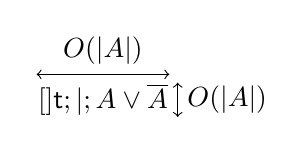
\begin{tikzpicture}[
			squarednode/.style={rectangle, draw=white, minimum size=5mm},
			textnode/.style={rectangle, draw=white}
			]
			%Nodes
			\node[squarednode]      (derivation) {$\drv[] {
					\trueUnit ; | ; A \lor \overline{A}
			}$};
			
			%Lines
			\draw[<->, shorten >= 3pt, shorten <= 3pt] (derivation.north west) to node[above, align=center] {$O(| A |)$} (derivation.north east);
			\draw[<->, shorten >= 3pt, shorten <= 3pt] (derivation.north east) to node[right, align=left] {$O(| A |)$} (derivation.south east);
		\end{tikzpicture}
	\end{center}
	Note also that occurrences of the quantifier-shifts $\rOneDown$ and $\rOneUp$ are included in the decomposed derivation if the instance of the inference rule contains quantifiers.
	
	\begin{lemma}\label{IdentityDecomposition}
		For every instance of the rule $\iDown$ of the form
		\[
		\drv[] {
			\trueUnit ; [\iDown]- ; A \lor \overline{A}
		}
		\]
		there exists a derivation
		\[
		\drv[] {
			\trueUnit ; [\phi]|[\{\aiDown, \switch, \exists, \rOneDown, \eqProp, \eqExists\}] ; A \lor \overline{A}
		}
		\]
		such that $\phi$ does not contain any occurrences of $=$ rules of the form $\drv[] {\exists x \exists y B ; [=]- ; \exists y \exists x B}$ or $\drv[] {B ; [=]- ; \exists x B}$ and $| \phi | = O(| A |^2)$. Furthermore, if $A$ is epsilon-free then $\phi$ may be chosen to be epsilon-free.
		
		Dually, for every instance of the rule $\iUp$ of the form
		\[
		\drv[] {
			A \land \overline{A} ; [\iUp]- ; \falseUnit
		}
		\]
		there exists a derivation
		\[
		\drv[] {
			A \land \overline{A} ; [\phi]|[\{\aiUp, \switch, \forall, \rOneUp, \eqProp, \eqForall\}] ; \falseUnit
		}
		\]
		such that $\phi$ does not contain any occurrences of $=$ rules of the form $\drv[] {\forall x \forall y B ; [=]- ; \forall y \forall x B}$ or $\drv[] {\forall x B ; [=]- ; B}$ and $| \phi | = O(| A |^2)$. Furthermore, if $A$ is epsilon-free then $\phi$ may be chosen to be epsilon-free.
	\end{lemma}
	
	\begin{proof}
		I present derivations for decomposing $\iDown$ rule instances by structural induction. $\iUp$ rule instances may be decomposed dually.
		
		For all formulae $A$, let $D(A)$ denote the derivation in $\SKSqDecomp$ obtained by decomposing the rule instance $\drv[] {\trueUnit ; [\iDown]- ; A \lor \overline{A}}$. For all formulae $A$ and $B$, all atomic formulae $a$ and all variables $x$, we have
		
		\[
		D(A \lor B) \hspace{1em} = \hspace{1em} \drv[] {
			\trueUnit ; [=]- ; \drv[border=black] {
				\drv[border=black] {
					\trueUnit ; [D(A)]| ; A \lor \overline{A}
				} \land \drv[border=black] {
					\trueUnit ; [D(B)]| ; B \lor \overline{B}
				}
			} ; |[\{\switch\}] ; (A \lor B) \lor (\overline{A} \land \overline{B})
		}
		\]
		so that $| D(A \lor B) | \leq k_1| A \lor B | + | D(A) | + | D(B) |$ for some constant $k_1$.
		
		\[
		D(A \land B) \hspace{1em} = \hspace{1em} \drv[] {
			\trueUnit ; [=]- ; \drv[border=black] {
				\drv[border=black] {
					\trueUnit ; [D(A)]| ; A \lor \overline{A}
				} \land \drv[border=black] {
					\trueUnit ; [D(B)]| ; B \lor \overline{B}
				}
			} ; |[\{\switch\}] ; (A \land B) \lor (\overline{A} \lor \overline{B})
		}
		\]
		so that $| D(A \land B) | \leq k_2 | A \land B | + | D(A) | + | D(B) |$ for some constant $k_2$.
		
		\[
		D(\forall x A(x)) \hspace{1em} = \hspace{1em} \drv[] {
			\forall x \, \drv[border=black] {
				\trueUnit ; [D(A(x))]| ; \drv[border=black] {
					A(x) \lor \drv[border=black] {
						\overline{A}(x) ; [\exists]- ; \exists y \overline{A}(y)
					}
				}
			} ; [\rOneDown]- ; \drv[border=black] {
				\forall x A(x) \lor \drv[border=black] {
					\exists y \overline{A}(y) ; [=]- ; \exists x \overline{A}(x)
				}
			}
		}
		\]
		where $y$ is some variable term that is free for $x$ in $A(x)$, so that $| D(\forall x A(x)) | \leq k_3 | \forall x A(x) | + | D(A(x)) |$ for some constant $k_3$.
		
		\[
		D(\exists x A(x)) \hspace{1em} = \hspace{1em} \drv[] {
			\forall x \, \drv[border=black] {
				\trueUnit ; [D(A(x))]| ; \drv[border=black] {
					\drv[border=black] {
						A(x) ; [\exists]- ; \exists y A(y)
					} \lor \overline{A}(x)
				}
			} ; [\rOneDown]- ; \drv[border=black] {
				\drv[border=black] {
					\exists y A(y) ; [=]- ; \exists x A(x)
				} \lor \forall x \overline{A}(x)
			}
		}
		\]
		where $y$ is some variable term that is free for $x$ in $A(x)$, so that $| D(\exists x A(x)) | \leq k_4 | \exists x A(x) | + | D(A(x)) |$ for some constant $k_4$.
		
		\[
		D(\trueUnit) \hspace{1em} = \hspace{1em} \drv[] {
			\trueUnit ; [=]- ; \trueUnit \lor \falseUnit
		}
		\]
		so that $| D(\trueUnit) | = 4$.
		
		\[
		D(\falseUnit) \hspace{1em} = \hspace{1em} \drv[] {
			\trueUnit ; [=]- ; \falseUnit \lor \trueUnit
		}
		\]
		so that $| D(\falseUnit) | = 4$.
		
		\[
		D(a) \hspace{1em} = \hspace{1em} \drv[] {
			\trueUnit ; [\aiDown]- ; a \lor \overline{a}
		}
		\]
		so that $| D(a) | = 2 | a | + 2$.
		
		It follows by appropriate choice of constant $K$ that for all formulae $A$, $| D(A) | \leq K| A |^2$. The result follows.
	\end{proof}
	
	The following lemma provides a decomposition of instances of the contraction rule $\cDown$ and its dual the cocontraction rule $\cUp$ into derivations in $\SKSqDecomp$. The derivation resulting from decomposing an instance
	\[
	\drv[] {
		A \lor A ; [\cDown]- ; A
	}
	\]
	of $\cDown$ (or, dually, $\cUp$) is of size $O(| A |^2)$ since the derivation is of height $O(| A |)$ due to each symbol in $A$ inducing a fixed-size subderivation in the decomposed derivation:
	\begin{center}
		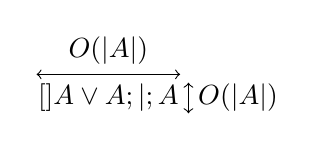
\begin{tikzpicture}[
			squarednode/.style={rectangle, draw=white, minimum size=5mm},
			textnode/.style={rectangle, draw=white}
			]
			%Nodes
			\node[squarednode]      (derivation) {$\drv[] {
					A \lor A ; | ; A
				}$};
			
			%Lines
			\draw[<->, shorten >= 3pt, shorten <= 3pt] (derivation.north west) to node[above, align=center] {$O(| A |)$} (derivation.north east);
			\draw[<->, shorten >= 3pt, shorten <= 3pt] (derivation.north east) to node[right, align=left] {$O(| A |)$} (derivation.south east);
		\end{tikzpicture}
	\end{center}
	The lemma also provides bounds for the number of occurrences of the existential contraction rule $\qcDown$ and universal cocontraction rule $\qcUp$ in the decomposed derivations, as this information will be relevant when assessing the complexity of the procedure for proving Theorem \ref{FalsifierNormalForm} the Falsifier Decomposition Theorem.
	
	\begin{lemma}\label{ContractionDecomposition}
		For every instance of the rule $\cDown$ of the form
		\[
		\drv[] {
			A \lor A ; [\cDown]- ; A
		}
		\]
		there exists a derivation
		\[
		\drv[] {
			A \lor A ; [\phi]|[\{\acDown, \medial, \qcDown, \forall, \eqProp, \eqForall\}] ; A
		}
		\]
		such that $\phi$ does not contain any occurrences of $=$ rules of the form $\drv[] {\forall x \forall y B ; [=]- ; \forall y \forall x B}$ or $\drv[] {\forall x B ; [=]- ; B}$, $| \phi | = O(| A |^2)$, $\phi$ contains at most $n$ occurrences of $\qcDown$, where $n$ is the number of existential quantifiers in $A$ which occur outside the scope of epsilon symbols, and the occurrences of $\qcDown$ in $\phi$ occur in parallel in $\phi$. Furthermore, if $A$ is epsilon-free then $\phi$ may be chosen to be epsilon-free.
		
		Dually, for every instance of the rule $\cUp$ of the form
		\[
		\drv[] {
			A ; [\cUp]- ; A \land A
		}
		\]
		there exists a derivation
		\[
		\drv[] {
			A ; [\phi]|[\{\acUp, \medial, \qcUp, \exists, \eqProp, \eqExists\}] ; A \land A
		}
		\]
		such that $\phi$ does not contain any occurrences of $=$ rules of the form $\drv[] {\exists x \exists y B ; [=]- ; \exists y \exists x B}$ or $\drv[] {B ; [=]- ; \exists x B}$, does not contain any occurrences of $\exists$ or $\eqExists$ if $A$ is weakly existential-free, $| \phi | = O(| A |^2)$, $\phi$ contains at most $n$ occurrences of $\qcUp$, where $n$ is the number of universal quantifiers in $A$ which occur outside the scope of epsilon symbols, and the occurrences of $\qcUp$ in $\phi$ occur in parallel in $\phi$. Furthermore, if $A$ is epsilon-free then $\phi$ may be chosen to be epsilon-free.
	\end{lemma}
	
	\begin{proof}
		I present derivations for decomposing $\cDown$ rule instances by structural induction. $\cUp$ rule instances may be decomposed dually.
		
		For all formulae $A$, let $D(A)$ denote the derivation in $\SKSqDecomp$ obtained by decomposing the rule instance $\drv[] {A \lor A ; [\cDown]- ; A}$. For all formulae $A$ and $B$, all atomic formulae $a$ and all variables $x$, we have
		
		\[
		D(A \lor B) \hspace{1em} = \hspace{1em} \drv[] {
			(A \lor B) \lor (A \lor B) ; [=]- ; \drv[border=black] {
				\drv[border=black] {A \lor A ; [D(A)]| ; A} \lor \drv[border=black] {B \lor B ; [D(B)]| ; B}
			}
		}
		\]
		so that $| D(A \lor B) | \leq k_1| A \lor B | + | D(A) | + | D(B) |$ for some constant $k_1$ and $D(A \lor B)$ contains $n + m$ occurrences of $\qcDown$, where $n$ is the number of occurrences of $\qcDown$ in $D(A)$ and $m$ is the number of occurrences of $\qcDown$ in $D(B)$. It also follows from the derivation above that if all occurrences of $\qcDown$ in $D(A)$ occur in parallel in $D(A)$ and all occurrences of $\qcDown$ in $D(B)$ occur in parallel in $D(B)$, then all occurrences of $\qcDown$ in $D(A \lor B)$ occur in parallel in $D(A \lor B)$.
		
		\[
		D(A \land B) \hspace{1em} = \hspace{1em} \drv[] {
			(A \land B) \lor (A \land B) ; [\medial]- ; \drv[border=black] {
				\drv[border=black] {A \lor A ; [D(A)]| ; A} \land \drv[border=black] {B \lor B ; [D(B)]| ; B}
			}
		}
		\]
		so that $| D(A \land B) | = 2| A \land B | + 2 + | D(A) | + | D(B) |$ and $D(A \land B)$ contains $n + m$ occurrences of $\qcDown$, where $n$ is the number of occurrences of $\qcDown$ in $D(A)$ and $m$ is the number of occurrences of $\qcDown$ in $D(B)$. It also follows from the derivation above that if all occurrences of $\qcDown$ in $D(A)$ occur in parallel in $D(A)$ and all occurrences of $\qcDown$ in $D(B)$ occur in parallel in $D(B)$, then all occurrences of $\qcDown$ in $D(A \land B)$ occur in parallel in $D(A \land B)$.
		
		\[
		D(\forall x A) \hspace{1em} = \hspace{1em} \drv[] {
			\forall x A \lor \forall x A ; [=]- ; \forall x \, \drv[border=black] {
				\drv[border=black] { \drv[border=black] {
						\forall y (A[y / x]) ; [\forall]- ; A
					} \lor \drv[border=black] {
						\forall y (A[y / x]) ; [\forall]- ; A
				} } ; [D(A)]| ; A
			}
		}
		\]
		where $y$ is some variable term that is free for $x$ in $A$, so that $| D(\forall x A) | \leq k_2| \forall x A | + | D(A) |$ for some constant $k_2$ and $D(\forall x A)$ contains the same number of occurrences of $\qcDown$ as $D(A)$. It also follows from the derivation above that if all occurrences of $\qcDown$ in $D(A)$ occur in parallel in $D(A)$, then all occurrences of $\qcDown$ in $D(\forall x A)$ occur in parallel in $D(\forall x A)$.
		
		\[
		D(\exists x A) \hspace{1em} = \hspace{1em} \drv[] {
			\exists x A \lor \exists x A ; [\qcDown]- ; \exists x A
		}
		\]
		so that $| D(\exists x A) | = 3 | \exists x A |$ and $D(\exists x A)$ contains precisely one occurrence of $\qcDown$.
		
		\[
		D(\trueUnit) \hspace{1em} = \hspace{1em} \drv[] {
			\trueUnit \lor \trueUnit ; [=]- ; \trueUnit
		}
		\]
		so that $| D(\trueUnit) | = 4$ and $D(\trueUnit)$ contains no occurrences of $\qcDown$.
		
		\[
		D(\falseUnit) \hspace{1em} = \hspace{1em} \drv[] {
			\falseUnit \lor \falseUnit ; [=]- ; \falseUnit
		}
		\]
		so that $| D(\falseUnit) | = 4$ and $D(\falseUnit)$ contains no occurrences of $\qcDown$.
		
		\[
		D(a) \hspace{1em} = \hspace{1em} \drv[] {
			a \lor a ; [\acDown]- ; a
		}
		\]
		so that $| D(a) | = 3 | a | + 1$ and $D(a)$ contains no occurrences of $\qcDown$.
		
		It follows by appropriate choice of constant $K$ that for all formulae $A$, $| D(A) | \leq K| A |^2$ and that $D(A)$ contains at most $n$ occurrences of $\qcDown$, where $n$ is the number of existential quantifiers in $A$ which occur outside the scope of epsilon symbols. Furthermore, all occurrences of $\qcDown$ in $D(A)$ occur in parallel in $D(A)$. The result follows.
	\end{proof}
	
	The following lemma provides a decomposition of instances of the weakening rule $\wDown$ and its dual the coweakening rule $\wUp$ into derivations in $\SKSqDecomp$. The derivation resulting from decomposing an instance
	\[
	\drv[] {
		\falseUnit ; [\wDown]- ; A
	}
	\]
	of $\wDown$ (or, dually, $\wUp$) is of size $O(| A |)$ since the derivation is of constant height due to each symbol in $A$ inducing a constant-size subderivation in the decomposed derivation:
	\begin{center}
		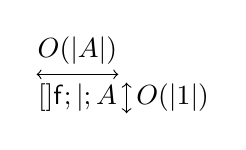
\begin{tikzpicture}[
			squarednode/.style={rectangle, draw=white, minimum size=5mm},
			textnode/.style={rectangle, draw=white}
			]
			%Nodes
			\node[squarednode]      (derivation) {$\drv[] {
					\falseUnit ; | ; A
				}$};
			
			%Lines
			\draw[<->, shorten >= 3pt, shorten <= 3pt] (derivation.north west) to node[above, align=center] {$O(| A |)$} (derivation.north east);
			\draw[<->, shorten >= 3pt, shorten <= 3pt] (derivation.north east) to node[right, align=left] {$O(| 1 |)$} (derivation.south east);
		\end{tikzpicture}
	\end{center}
	
	\begin{lemma}\label{WeakeningDecomposition}
		For every instance of the rule $\wDown$ of the form
		\[
		\drv[] {
			\falseUnit ; [\wDown]- ; A
		}
		\]
		there exists a derivation
		\[
		\drv[] {
			\falseUnit ; [\phi]|[\{\awDown, \exists, \eqProp, \eqForall\}] ; A
		}
		\]
		such that $\phi$ does not contain any occurrences of $=$ rules of the form $\drv[] {\forall x \forall y B ; [=]- ; \forall y \forall x B}$, $\drv[] {\forall x B ; [=]- ; B}$ and $| \phi | = O(|A|)$. Furthermore, if $A$ is epsilon-free then $\phi$ may be chosen to be epsilon-free.
		
		Dually, for every instance of the rule $\wUp$ of the form
		\[
		\drv[] {
			A ; [\wUp]- ; \trueUnit
		}
		\]
		there exists a derivation
		\[
		\drv[] {
			A ; |[\{\awUp, \forall, \eqProp, \eqExists\}] ; \trueUnit
		}
		\]
		such that $\phi$ does not contain any occurrences of $=$ rules of the form $\drv[] {\exists x \exists y B ; [=]- ; \exists y \exists x B}$ or $\drv[] {B ; [=]- ; \exists x B}$, does not contain any occurrences of $\eqExists$ if $A$ is weakly existential-free and $| \phi | = O(|A|)$. Furthermore, if $A$ is epsilon-free then $\phi$ may be chosen to be epsilon-free.
	\end{lemma}
	
	\begin{proof}
		I present derivations for decomposing $\wDown$ rule instances by structural induction. $\wUp$ rule instances may be decomposed dually.
		
		For all formulae $A$, let $D(A)$ denote the derivation in $\SKSqDecomp$ obtained by decomposing the rule instance $\drv[] {\falseUnit ; [\wDown]- ; A}$. For all formulae $A$ and $B$, all atomic formulae $a$ and all variables $x$, we have
		
		\[
		D(A \lor B) \hspace{1em} = \hspace{1em} \drv[] {
			\falseUnit ; [=]- ; \drv[border=black] {
				\drv[border=black] {
					\falseUnit ; [D(A)]| ; A
				} \lor \drv[border=black] {
					\falseUnit ; [D(B)]| ; B
				}
			}
		}
		\]
		so that $| D(A \lor B) | = 2 + | D(A) | + | D(B) |$.
		
		\[
		D(A \land B) \hspace{1em} = \hspace{1em} \drv[] {
			\falseUnit ; [=]- ; \drv[border=black] {
				\drv[border=black] {
					\falseUnit ; [D(A)]| ; A
				} \land \drv[border=black] {
					\falseUnit ; [D(B)]| ; B
				}
			}
		}
		\]
		so that $| D(A \land B) | = 2 + | D(A) | + | D(B) |$.
		
		\[
		D(\forall x A) \hspace{1em} = \hspace{1em} \drv[] {
			\falseUnit ; [=]- ; \forall x \, \drv[border=black] {
				\falseUnit ; [D(A)]| ; A
			}
		}
		\]
		so that $| D(\forall x A) | = 2 + | D(A) |$.
		
		\[
		D(\exists x A) \hspace{1em} = \hspace{1em} \drv[] {
			\falseUnit ; [\exists]- ; \exists x \, \drv[border=black] {
				\falseUnit ; [D(A)]| ; A
			}
		}
		\]
		so that $| D(\exists x A) | = 2 + | D(A) |$.
		
		\[
		D(\trueUnit) \hspace{1em} = \hspace{1em} \drv[] {
			\falseUnit ; [\awDown]- ; \trueUnit
		}
		\]
		so that $| D(\trueUnit) | = 2$.
		
		\[
		D(\falseUnit) \hspace{1em} = \hspace{1em} \falseUnit
		\]
		so that $| D(\falseUnit) | = 1$.
		
		\[
		D(a) \hspace{1em} = \hspace{1em} \drv[] {
			\falseUnit ; [\awDown]- ; a
		}
		\]
		so that $| D(a) | = 1 + | a |$.
		
		It follows by appropriate choice of constant $K$ that for all formulae $A$, $| D(A) | \leq K| A |$. The result follows.
	\end{proof}
	
	The following lemma provides decompositions of instances of the equality rules which are contained in $\SKSq$ but not $\SKSqDecomp$ into derivations in $\SKSqDecomp$.
	
	\begin{lemma}\label{EqualityDecomposition}
		For every instance
		\[
		\drv[] {
			A ; [=]- ; B
		}
		\]
		of an inference rule of the form $\drv[] {\exists x \exists y C ; [=]- ; \exists y \exists x C}$, $\drv[] {\forall x \forall y C ; [=]- ; \forall y \forall x C}$, $\drv[] {C ; [=]- ; \exists x C}$ or $\drv[] {\forall x C ; [=]- ; C}$, there exists a derivation
		\[
		\drv[] {
			A ; [\phi]|[\{\exists, \forall, \eqExists, \eqForall\}] ; B
		}
		\]
		such that $\phi$ does not contain any occurrences of $=$ rules of the form $\drv[] {\exists x \exists y C ; [=]- ; \exists y \exists x C}$, $\drv[] {\forall x \forall y C ; [=]- ; \forall y \forall x C}$, $\drv[] {C ; [=]- ; \exists x C}$ or $\drv[] {\forall x C ; [=]- ; C}$ and $| \phi | = O(| A |)$. Furthermore, if $A$ is epsilon-free then $\phi$ may be chosen to be epsilon-free.
	\end{lemma}
	
	\begin{proof}
		I present derivations for each inference rule.
		
		\[
		\drv[] {
			\exists x \exists y C ; [=]- ; \exists y \exists x C
		} \hspace{2em} \rightarrow \hspace{2em} \drv[] {
			\drv[border=black] {
				\exists x \exists y \, \drv[border=black] {
					C ; [\exists]- ; \exists x C
				} 
			} ; [=]- ; \exists y \exists x C
		}
		\]
		
		\[
		\drv[] {
			\forall x \forall y C ; [=]- ; \forall y \forall x C
		} \hspace{2em} \rightarrow \hspace{2em} \drv[] {
			\forall x \forall y C ; [=]- ; \drv[border=black] {
				\forall y \forall x \, \drv[border=black] {
					\forall y C ; [\forall]- ; C
				}
			}
		}
		\]
		
		\[
		\drv[] {
			C ; [=]- ; \exists x C
		} \hspace{2em} \rightarrow \hspace{2em} \drv[] {
			C ; [\exists]- ; \exists x C
		}
		\]
		
		\[
		\drv[] {
			\forall x C ; [=]- ; C
		} \hspace{2em} \rightarrow \hspace{2em} \drv[] {
			\forall x C ; [\forall]- ; C
		}
		\]
	\end{proof}
	
	Remarkably, in a deep-inference setting, most of the quantifier-shift rules are trivial, in that they may be decomposed into derivations in $\SKSqDecomp$ with linear complexity. The following proposition demonstrates that, with the exceptions of $\rOneDown$ and $\rOneUp$, instances of the quantifier-shifts in $\SKSq$ may be decomposed into derivations in $\SKSqDecomp \setminus \{\rOneDown, \rOneUp\}$ with linear complexity. This resembles the equivalence of quantifier-shifts and traditional first-order deep-inference rules that is observed in Ralph's thesis \cite{BenThesis}. The consequences of this fact and the properties of the non-trivial quantifier-shifts $\rOneDown$ and $\rOneUp$ will be explored in more detail in the following two subsections, Subsections \ref{QuantifierShiftsSection} and \ref{CaseAnalysisExtractionSection}.
	
	\begin{proposition}[Decomposition of quantifier-shifts]\label{RemoveROP}
		For every instance $\drv[] {A ; [\rho]- ; B}$ of an inference rule $\rho \in \{\rTwoDown, \rTwoUp, \rThreeDown, \rThreeUp, \rFourDown, \rFourUp\}$, there exists a derivation
		\[
		\drv[] {
			A ; [\phi]|[\{\awDown, \awUp, \qcDown, \qcUp, \exists, \forall, \eqProp, \eqExists, \eqForall\}] ; B
		}
		\]
		such that $\phi$ does not contain any occurrences of $=$ rules of the form $\drv[] {\exists x \exists y C ; [=]- ; \exists y \exists x C}$, $\drv[] {\forall x \forall y C ; [=]- ; \forall y \forall x C}$, $\drv[] {C ; [=]- ; \exists x C}$ or $\drv[] {\forall x C ; [=]- ; C}$ and $| \phi | = O(| A |)$. Furthermore, if $A$ is epsilon-free then $\phi$ may be chosen to be epsilon-free.
	\end{proposition}
	
	\begin{proof}
		I present derivations for $\rTwoDown$, $\rThreeDown$ and $\rFourDown$. The remaining rules may be derived dually.
		
		\[
		\drv[] {
			\forall x (A(x) \land B) ; [\rTwoDown]- ; \forall x A(x) \land B
		} \hspace{2em} \rightarrow \hspace{2em} \drv[] {
			\forall x (A(x) \land B) ; [\qcUp]- ; \drv[border=black] { \forall x \, \drv[border=black] {
					A(x) \land \drv[border=black] {B ; [\wUp]- ; \trueUnit}
				} \land \drv[border=black] {
					\forall x \, \drv[border=black] {
						\drv[border=black] {A(x) ; [\wUp]- ; \trueUnit} \land B
					} ; [\forall]- ; \trueUnit \land B
				} ; [=]- ; \forall x A(x) \land B
			}
		}
		\]
		where the occurrences of $\wUp$ in the derivation above are replaced with derivations in $\{\awUp, \forall, \eqProp, \eqExists\}$ using Lemma \ref{WeakeningDecomposition} and sequential composition.
		
		\[
		\drv[] {
			\exists x (A(x) \lor B) ; [\rThreeDown]- ; \exists x A(x) \lor B
		} \hspace{2em} \rightarrow \hspace{2em} \drv[] {
			\exists x \, \drv[border=black] {
				\drv[border=black] {
					A(x) ; [\exists]- ; \exists y A(y)
				} \lor B
			} ; [=]- ; \exists x A(x) \lor B
		}
		\]
		where $y$ is some variable that is free for $x$ in $A(x)$.
		
		\[
		\drv[] {
			\exists x (A(x) \land B) ; [\rFourDown]- ; \exists x A(x) \land B
		} \hspace{2em} \rightarrow \hspace{2em} \drv[] {
			\exists x \, \drv[border=black] {
				\drv[border=black] {
					A(x) ; [\exists]- ; \exists y A(y)
				} \land B
			} ; [=]- ; \exists x A(x) \land B
		}
		\]
		where $y$ is some variable that is free for $x$ in $A(x)$.
		
		Observe that the size of each construction is linear with respect to the size of the premise of each inference rule. The result follows.
	\end{proof}

	The following lemma combines the above results to provide a full decomposition from derivations in $\SKSq$ to derivations in $\SKSqDecomp$.
	
	\begin{lemma}\label{DecompositionToSKSqDecompFull}
		For every derivation
		\[
			\drv[] {
				A ; [\phi]|[\SKSq] ; B
			}
		\]
		there exists a derivation
		\[
			\drv[] {
				A ; [\phi']|[\SKSqDecomp] ; B
			}
		\]
		such that $| \phi' | = O(| \phi |^2)$. Furthermore, if $\phi$ is epsilon-free then $\phi'$ may be chosen to be epsilon-free and if $\phi$ is cut-free then $\phi'$ may be chosen to be cut-free.
	\end{lemma}
	
	\begin{proof}
		By replacing all occurrences of inference rules in $\SKSq \setminus \SKSqDecomp$ in $\phi$ with derivations in $\SKSqDecomp$ using sequential composition, by Lemmas \ref{IdentityDecomposition}, \ref{ContractionDecomposition}, \ref{WeakeningDecomposition} and \ref{EqualityDecomposition} and Proposition \ref{RemoveROP}.
	\end{proof}
	
	\subsection{Quantifier-Shifts and Non-Elementary Compression}\label{QuantifierShiftsSection}
	
	Of particular interest in the study of first-order proof complexity and normalisation are the inference rules in $\SKSq$ known as \textit{quantifier-shifts}, which are given by\vspace{0.5em}
	
	{\centering
		\begin{tabular} { | c c c c | }
			\hline
			& & & \\
			$\hspace{1em}\drv[] {\forall x (A(x) \lor B) ; [\rOneDown]- ; \forall x A(x) \lor B}$ &
			$\drv[] {\forall x (A(x) \land B) ; [\rTwoDown]- ; \forall x A(x) \land B}$ &
			$\drv[] {\exists x (A(x) \lor B) ; [\rThreeDown]- ; \exists x A(x) \lor B}$ &
			$\drv[] {\exists x (A(x) \land B) ; [\rFourDown]- ; \exists x A(x) \land B}\hspace{1em}$ \\
			& & & \\
			$\hspace{1em}\drv[] {\exists x A(x) \land B ; [\rOneUp]- ; \exists x (A(x) \land B)}$ &
			$\drv[] {\exists x A(x) \lor B ; [\rTwoUp]- ; \exists x (A(x) \lor B)}$ &
			$\drv[] {\forall x A(x) \land B ; [\rThreeUp]- ; \forall x (A(x) \land B)}$ &
			$\drv[] {\forall x A(x) \lor B ; [\rFourUp]- ; \forall x (A(x) \lor B)}\hspace{1em}$ \\
			& & &  \\
			\hline
		\end{tabular}
		\par}
	
	\vspace{0.5em}
	\noindent where $x$ does not occur free in $B$.
	
	The quantifier-shifts were first introduced in Herbrand's thesis in 1929 \cite{HerbrandThesis} to be used as part of his proof of Herbrand's Theorem under the name of ``rules of passage". Herbrand's thesis also included quantifier-shifts for shifting negation symbols $\neg$ inside and outside of quantifiers, given by\vspace{0.5em}
	
	{\centering
		\begin{tabular} { | c c c c | }
			\hline
			& & & \\
			$\hspace{1em}\drv[] {\neg \forall x A ; - ; \exists x \neg A}$ &
			$\drv[] {\neg \exists x A ; - ; \forall x \neg A}$ &
			$\drv[] {\exists x \neg A ; - ; \neg \forall x A}$ &
			$\drv[] {\forall x \neg A ; - ; \neg \exists x A}\hspace{1em}$ \\
			& & & \\
			\hline
		\end{tabular}
		\par}
	
	\vspace{0.5em}
	\noindent and it is sometimes also convenient to consider variants of the quantifier-shifts for implication $\rightarrow$ which are generated by the classical logical equivalence $A \rightarrow B \equiv \overline{A} \lor B$ and are given by\vspace{0.5em}
	
	{\centering
		\begin{tabular} { | c c c c | }
			\hline
			& & & \\
			$\hspace{1em}\drv[] {\forall x (A(x) \rightarrow B) ; - ; \exists x A(x) \rightarrow B}$ &
			$\drv[] {\exists x (A(x) \rightarrow B) ; - ; \forall x A(x) \rightarrow B}$ &
			$\drv[] {\forall x (B \rightarrow A(x)) ; - ; B \rightarrow \forall x A(x)}$ &
			$\drv[] {\exists x (B \rightarrow A(x)) ; - ; B \rightarrow \exists x A(x)}\hspace{1em}$ \\
			& & & \\
			$\hspace{1em}\drv[] {\exists x A(x) \rightarrow B ; - ; \forall x (A(x) \rightarrow B)}$ &
			$\drv[] {\forall x A(x) \rightarrow B ; - ; \exists x (A(x) \rightarrow B)}$ &
			$\drv[] {B \rightarrow \forall x A(x) ; - ; \forall x (B \rightarrow A(x))}$ &
			$\drv[] {B \rightarrow \exists x A(x) ; - ; \exists x (B \rightarrow A(x))}\hspace{1em}$ \\
			& & &  \\
			\hline
		\end{tabular}
		\par}
	
	\vspace{0.5em}
	\noindent where $x$ does not occur free in $B$. The quantifier-shifts were in fact the source of an error in Herbrand's thesis, which was discovered and corrected by Aanderaa, Andrews and Dreben in 1963 \cite{DrebenFalseLemmasInHerbrand}.
	
	A remarkable phenomenon in first-order proof theory is that some proof systems admit non-elementarily smaller cut-free proofs of certain classes of theorems than other proof systems. In \cite{StatmanLowerBounds}, Statman provides a class $S$ of first-order theorems for which there is no elementary function bounding the size of the smallest Herbrand disjunction for a formula in $S$ in terms of the size of its smallest proof in Gentzen's sequent calculus $\textbf{LK}$. In \cite{BaazUnsoundInferences}, Aguilera and Baaz define a sequent-calculus proof system $\textbf{LK}_{shift}$ which is obtained by extending $\textbf{LK}$ by the quantifier-shift rules in $\SKSq$ and those for implication and demonstrate that for a class $S'$ of first-order theorems obtained by adapting $S$, there is no elementary function bounding the size of the smallest cut-free $\textbf{LK}$ proof of a formula in $S'$ in terms of the size of its smallest cut-free $\textbf{LK}_{shift}$ proof. Notably, the sequent-calculus-based epsilon-calculus also admits this compression over the sequent calculus for cut-free proofs \cite{BaazLolicEpsilonShorterProofs} since critical axioms can simulate quantifier-shifts in the presence of the encodings of quantifiers by $\varepsilon$-terms. Since the quantifier-shifts involve rewriting inside a formula, they are natural deep-inference inference rules and it follows that deep-inference proof systems for first-order predicate logic admit non-elementarily smaller cut-free proofs than $\textbf{LK}$ for certain classes of theorems (see Proposition \ref{SKSqSpeedupOverLK}). The non-elementary compression of cut-free proofs in deep inference arising from the quantifier-shifts is also discussed in Ralph's thesis \cite{BenThesis}. Given the finer granularity of inference rules and more flexible composition mechanism exhibited by open deduction over the sequent calculus, it is natural to consider what properties of the quantifier-shifts may be revealed by analysing them in the open deduction formalism and what insights this might provide into the properties which make a proof system admit the non-elementary compression over the sequent calculus for cut-free proofs.
	
	As was demonstrated by Proposition \ref{RemoveROP}, most of the quantifier-shifts are trivial in open deduction, in that they may be decomposed into derivations in $\SKSqDecomp \setminus \{\rOneDown, \rOneUp\}$ with linear complexity. The quantifier-shifts $\rOneDown$ and $\rOneUp$, however, are more delicate and do not admit such decompositions, warranting a closer analysis of these rules and the role they play in the phenomenon of the non-elementary compression of cut-free proofs. As was noted in Lemma \ref{IdentityDecomposition}, instances of the identity rule $\iDown$ may be decomposed into derivations in $\{\aiDown, \switch, \exists, \rOneDown, \eqProp, \eqExists, \eqForall\}$ and, dually, instances of the cut rule $\iUp$ may be decomposed into derivations in $\{\aiUp, \switch, \forall, \rOneUp, \eqProp, \eqExists, \eqForall\}$, establishing connections between the identity rule $\iDown$ and the quantifier-shift $\rOneDown$ and between the cut rule $\iUp$ and the quantifier-shift $\rOneUp$. More specifically, an instance of the identity rule $\iDown$ on a quantified formula $\forall x A(x)$ may be decomposed into an instance of the $\rOneDown$ quantifier-shift, an instance of the existential witnessing rule $\exists$ and an instance of the identity rule $\iDown$ on the formula $A(x)$:
	\[
	\drv[] {
		\trueUnit ; [\iDown]- ; \forall x A(x) \lor \exists x \overline{A}(x)
	} \hspace{1em} \rightarrow \hspace{1em} \drv[] {
		\trueUnit ; [=]- ; \forall x \, \drv[border=black] {
			\trueUnit ; [\iDown]- ; \drv[border=black] {
				A(x) \lor \drv[border=black] {
					\overline{A}(x) ; [\exists]- ; \exists y \overline{A}(y)
				}
			}
		} ; [\rOneDown]- ; \drv[border=black] {
			\forall x A(x) \lor \drv[border=black] {
				\exists y \overline{A}(y) ; [=]- ; \exists x \overline{A}(x)
			}
		}
	}
	\]
	and, dually, an instance of the cut rule $\iUp$ on a quantified formula $\forall x A(x)$ may be decomposed into an instance of the $\rOneUp$ quantifier-shift, an instance of the universal instantiation rule $\forall$ and an instance of the cut rule $\iUp$ on the formula $A(x)$:
	\[
	\drv[] {
		\forall x A(x) \land \exists x \overline{A}(x) ; [\iUp]- ; \falseUnit
	} \hspace{1em} \rightarrow \hspace{1em} \drv[] {
		\drv[border=black] {
			\drv[border=black] {
				\forall x A(x) ; [=]- ; \forall y A(y)
			} \land \exists x \overline{A}(x)
		} ; [\rOneUp]- ; \exists x \, \drv[border=black] {
			\drv[border=black] {
				\drv[border=black] {
					\forall y A(y) ; [\forall]- ; A(x)
				} \land \overline{A}(x)
			} ; [\iUp]- ; \falseUnit
		} ; [=]- ; \falseUnit
	}
	\]
	
	Given the fundamental roles of the identity rule $\iDown$ and the cut rule $\iUp$ in the proof theory of first-order predicate logic, these decomposition results suggest that the quantifier-shifts $\rOneDown$ and $\rOneUp$ share similarly important roles, hence why they do not admit trivial decompositions like the other quantifier-shifts. Indeed, this connects the elimination of occurrences of the quantifier-shifts $\rOneDown$ and $\rOneUp$ from a first-order proof to the non-trivial phenomenon of cut elimination and, consequently, Herbrand's Theorem. Both cut elimination \cite{BussIntroductionToProofTheory} and Herbrand's Theorem \cite{StatmanLowerBounds} are associated with non-elementary blowups in proof complexity, suggesting a fundamental connection between these theorems, the non-trivial quantifier-shifts $\rOneDown$ and $\rOneUp$ and the phenomenon of non-elementary proof compression. As will be discussed in the following subsection, Subsection \ref{CaseAnalysisExtractionSection}, the quantifier-shifts $\rOneDown$ and $\rOneUp$ also present certain challenges for the normalisation of first-order proofs when permuting occurrences of the existential contraction rule $\qcDown$ down a proof and occurrences of the universal cocontraction rule $\qcUp$ up a proof.
	
	Interestingly, the quantifier-shift $\rOneDown$, which is given by
	\[
	\drv[] {
		\forall x (A(x) \lor B) ; [\rOneDown]- ; \forall x A(x) \lor B
	}
	\]
	where $x$ does not occur free in $B$, is also the only quantifier-shift in $\SKSq$ which is not intuitionistically valid. The role of by quantifier-shifts in intuitionistic and intermediate logics has recently been studied by Baaz, Gamsakhurdia, Iemhoff and Jalali, who have demonstrated that an intermediate logic admits Skolemisation if and only if it admits all of the quantifier-shifts (including those for implication) \cite{BaazSkolemisationIntermediateLogics}.
	
	\subsection{Case Analysis Extraction and Herbrand's Theorem}\label{CaseAnalysisExtractionSection}
	
	In the proof theory of first-order predicate logic, contractions on existential formulae may be understood as case analyses on the witnesses to the existential quantifiers in the premise of the contraction:
	\[
	\drv[] {
		\textcolor{red}{\exists x} A \lor \textcolor{blue}{\exists x} A ; [\qcDown]- ; \textcolor{green}{\exists x} A
	}
	\]
	the witness to the existential quantifier $\textcolor{green}{\exists x}$ in the conclusion may be understood as a case analysis on the witness to the existential quantifier $\textcolor{red}{\exists x}$ on the left side of the disjunction in the premise and the witness to the existential quantifier $\textcolor{blue}{\exists x}$ on the right side of the disjunction in the premise. Dually, cocontractions on universal formulae 
	\[
	\drv[] {
		\forall x A ; [\qcUp]- ; \forall x A \land \forall x A
	}
	\]
	may also be understood as case analyses on the terms that instantiate the universal quantifiers in the conclusion later in a proof. A semantically natural operation to perform on a first-order proof is thus to extract the case analyses contained within such quantifier contraction rules from the proof, deriving a disjunction of terms which witness the existential quantifiers in the conclusion. This is one of the essential notions of \textit{Herbrand's Theorem} \cite{HerbrandThesis}, a fundamental theorem of classical proof theory, and the propositional disjunction collecting the term witnesses is called a \textit{Herbrand disjunction} for the conclusion of the proof.
	
	In the sequent calculus, Herbrand's Theorem is traditionally proved as a corollary to cut elimination, such as in an exposition of a proof of the general version of the theorem due to Buss \cite{BussIntroductionToProofTheory, BussHerbrand} (with a correction due to McKinley \cite{McKinleyBussCorrection}). In ``Buss-style" proofs of Herbrand's Theorem, cut rules are first eliminated from a sequent-calculus proof to make the proof amenable to rule permutations. Existential witnessing and existential contraction rules are then permuted down the cut-free proof to yield a propositional proof of a Herbrand disjunction for the conclusion of the proof.
	
	In a deep-inference setting, Brünnler \cite{KaiCutElimination} has presented a statement and proof of the general version of Herbrand's Theorem in the form of a decomposition theorem which does not require cuts to be eliminated from the proof, establishing a kind of independence between cut elimination and Herbrand's Theorem in deep inference which is not observable in the sequent calculus. Brünnler presents a procedure which transforms a first-order deep-inference proof into a factorised proof of the form
	\[
	\drv[] {
		\forall x_1 \dots \forall x_n \, \drv[border=black] {; T[\text{Propositional rules ($\SKSProp$)}] ; A'} ; |[\{\exists\}] ; A'' ; |[\{\rOneDown, \rTwoDown, \rThreeDown, \rFourDown\}] ; A''' ; |[\{\qcDown\}] ; A
	}
	\]
	where $A''$ is in prenex normal form, the formula $\forall x_1 \dots \forall x_n A'$ is a Herbrand disjunction for $A$ and the above proof is said to be in \textit{Herbrand normal form}.
	
	As was discussed in the previous subsection, Subsection \ref{QuantifierShiftsSection}, Statman \cite{StatmanLowerBounds} has shown that, in general, there is no elementary bound on the size of the smallest Herbrand disjunction for a first-order theorem in terms of the size of its smallest proof, which is related to the non-elementary compression of cut-free proofs yielded by proof systems which include quantifier-shifts. A natural question then is whether it is possible to extract the case analyses contained in quantifier contraction rules from a first-order proof without producing the non-elementary blowups incurred by Herbrand’s Theorem. This is possible using the central proof system of this thesis, the falsifier calculus, and is one of the essential notions of its corresponding decomposition theorem, Theorem \ref{FalsifierNormalForm} the Falsifier Decomposition Theorem, both of which will be introduced and explored in the following section, Section \ref{FalsifierCalculusSection}. I will first, however, consider this problem in the setting of the standard syntax of predicate logic and illustrate why such case analysis extraction with elementary complexity is not possible in standard first-order deep-inference proof systems such as $\SKSq$.
	
	In a deep-inference setting, to extract the case analyses contained within occurrences of the existential contraction rule $\qcDown$ from a first-order proof, the rule occurrences may be permuted down the proof by recursively permuting them down through the rule occurrences immediately below them until they reach the bottom of the proof. However, when an occurrence of $\qcDown$ is permuted down through certain occurrences of the $\rOneUp$ quantifier-shift, an occurrence of the universal cocontraction rule $\qcUp$, the dual of $\qcDown$, is introduced into the proof, as follows:
	\[
	\drv[] {
		\drv[border=black] {
			\drv[border=black] {\exists x A \lor \exists x A ; [\qcDown]- ; \exists x A} \land \forall y B
		} ; [\rOneUp]- ; \exists x (A \land \forall y B)
	} \hspace{2em} \rightarrow \hspace{2em} \drv[] {
		\drv[border=black] {(\exists x A \lor \exists x A) \land \drv[border=black,background=red!20] {\forall y B ; [\qcUp]- ; \forall y B \land \forall y B}} ; [=]- ; \drv[border=black] {
			\forall y B \land \drv[border=black] {
				\forall y B \land (\exists x A \lor \exists x A) ; [\switch]- ; (\exists x A \land \forall y B) \lor \exists x A
			}
		} ; [\switch]- ; \drv[border=black] {
			\drv[border=black] {\exists x A \land \forall y B ; [\rOneUp]- ; \exists x (A \land \forall y B)} \lor \drv[border=black] {\exists x A \land \forall y B ; [\rOneUp]- ; \exists x (A \land \forall y B)}
		} ; [\qcDown]- ; \exists x (A \land \forall y B)
	}
	\]
	
	Dually, when an occurrence of $\qcUp$ is permuted up through certain occurrences of the $\rOneDown$ quantifier-shift, an occurrence of $\qcDown$ is introduced into the proof, as follows:
	\begin{gather}\label{qcUpThroughRoneDownPermutation}
		\drv[] {
			\forall x (A \lor \exists y B) ; [\rOneDown]- ; \drv[border=black] {
				\drv[border=black] {\forall x A ; [\qcUp]- ; \forall x A \land \forall x A} \lor \exists y B
			}
		} \hspace{2em} \rightarrow \hspace{2em} \drv[] {
			\forall x (A \lor \exists y B) ; [\qcUp]- ; \drv[border=black] {
				\drv[border=black] {\forall x (A \lor \exists y B) ; [\rOneDown]- ; \forall x A \lor \exists y B} \land \drv[border=black] {\forall x (A \lor \exists y B) ; [\rOneDown]- ; \forall x A \lor \exists y B}
			} ; [\switch]- ; \drv[border=black] {
				\drv[border=black] {
					(\forall x A \lor \exists y B) \land \forall x A ; [\switch]- ; (\forall x A \land \forall x A) \lor \exists y B
				} \lor \exists y B
			} ; [=]- ; \drv[border=black] {
				(\forall x A \land \forall x A) \lor \drv[border=black,background=red!20] {\exists y B \lor \exists y B ; [\qcDown]- ; \exists y B}
			}
		}
	\end{gather}
	
	Consequently, a procedure which successively permutes occurrences of $\qcDown$ down and occurrences of $\qcUp$ up a first-order proof is non-terminating in the standard syntax of predicate logic. Consider, for instance, a proof which contains the following subderivation:
	\[
	\drv[] {
		\drv[border=black] {
			\drv[border=black] {
				\forall x (A \lor \exists y B) ; [\rOneDown]- ; \drv[border=black] {
					\drv[border=black] {\forall x A ; [\qcUp]- ; \forall x A \land \forall x A} \lor \exists y B
				}
			} \land C
		} ; [\switch]- ; (\forall x A \land \forall x A) \lor (\exists y B \land C) ; [\medial]- ; \drv[border=black] {
			\drv[border=black] {\forall x A \lor \exists y B ; [\rTwoUp]- ; \exists y (\forall x A \lor B)} \land (\forall x A \lor C)
		} ; [\rOneUp]- ; \exists y ((\forall x A \lor B) \land (\forall x A \lor C))
	}
	\]
	When the occurrence of $\qcUp$ is permuted up through the occurrence of $\rOneDown$ immediately above it, an occurrence of the existential contraction rule $\qcDown$ on the formula $\exists y B$ is introduced into the proof. If this occurrence of $\qcDown$ is subsequently permuted down the proof, when it is permuted down through the occurrence of $\rOneDown$ at the bottom of the subderivation, a further occurrence of $\qcUp$ is introduced into the proof. In this manner, each phase of permuting occurrences of $\qcUp$ up the proof will introduce further occurrences of $\qcDown$ into the proof and each phase of permuting occurrences of $\qcDown$ down the proof will introduce further occurrences of $\qcUp$ into the proof, resulting in non-termination.
	
	The following section, Section \ref{FalsifierCalculusSection}, introduces a proof system which is able to overcome these difficulties and attain termination of the procedure described above through the use of an inference rule which generalises the quantifier-shift $\rOneDown$ and introduces $\varepsilon$-terms into proofs. Through a certain normalisation, this system is able to avoid introducing unnecessary occurrences of $\qcDown$ into the proof during this procedure and instead introduces contractions on $\varepsilon$-terms, yielding termination. The resultant decomposition theorem is the central result of this thesis, Theorem \ref{FalsifierNormalForm} the Falsifier Decomposition Theorem, which is able to extract the case analyses contained in quantifier contraction rules from a first-order proof with elementary complexity due to the presence of $\varepsilon$-terms in the corresponding decomposed proofs.
	
	\pagebreak
	
	\section{The Falsifier Calculus}\label{FalsifierCalculusSection}
	
	\epigraph{Logic takes care of itself; all we have to do is to look and see how it does it.}{\textit{L. Wittgenstein}}
	
	\noindent
	The traditional epsilon-calculus as studied in Hilbert-Frege systems and the sequent calculus admits several notable and useful properties, such as admitting non-elementarily smaller cut-free proofs of certain classes of theorems than traditional proof systems \cite{BaazLolicEpsilonShorterProofs} and a rich proof theory, as encapsulated in the epsilon theorems \cite{MoserZachEpsilonCalculusAndHerbrand}. However, the traditional epsilon-calculus is notoriously unwieldy and these properties rely on the use of cumbersome encodings of quantifiers in proofs by $\varepsilon$-terms. In this section I will introduce the \textit{falsifier calculus}, an open-deduction proof system for first-order predicate logic in the language of the epsilon-calculus which exhibits the desirable properties of the traditional epsilon-calculus while simplifying some of its more unwieldy aspects and providing new insights into the structure and complexity of first-order proofs. The falsifier calculus uses a new inference rule to introduce $\varepsilon$-terms into proofs, called the \textit{falsifier rule} $\falsifierRule$, which is given by
	\[
	\drv[] {
		\forall x (A(x) \lor B(x)) ; [\falsifierRule]- ; \forall x A(x) \lor B(\varepsilon_y \overline{A}(y))
	}
	\]
	where $y$ is a variable such that $y$ is free for $x$ in $A(x)$ and $\varepsilon_y \overline{A}(y)$ is free for $x$ in $B(x)$, and is distinct from the critical axioms used to introduce $\varepsilon$-terms into proofs in the traditional epsilon-calculus. Through the use of the falsifier rule $\falsifierRule$, the falsifier calculus admits the non-elementary compression of cut-free proofs over the sequent calculus that is exhibited by the traditional epsilon-calculus, but without the need to encode quantifiers in proofs by $\varepsilon$-terms. The falsifier rule $\falsifierRule$ is a generalisation of the quantifier-shift $\rOneDown$, providing a new perspective on the non-elementary compression of cut-free proofs yielded by quantifier-shifts. Due to the presence of the falsifier rule $\varepsilon$ and the more expressive syntax of the epsilon-calculus, the falsifier calculus is also able to attain termination of the case analysis extraction procedure described in Subsection \ref{CaseAnalysisExtractionSection}, yielding a new decomposition theorem for proofs in first-order predicate logic and the central result of this thesis, Theorem \ref{FalsifierNormalForm} the Falsifier Decomposition Theorem. The Falsifier Decomposition Theorem decomposes a first-order proof into an upper segment of weakly existential-free formulae in the falsifier calculus and a lower segment of existential witnesses and existential contractions in $\{\exists, \qcDown\}$. The Falsifier Decomposition Theorem can be understood as an analogue to Herbrand's Theorem in which the upper segments of the corresponding proofs may be non-elementarily smaller than the corresponding smallest proofs in Herbrand normal form, providing insight into the role of $\varepsilon$-terms in the non-elementary compression of cut-free proofs.
	
	In Subsection \ref{FalsifierRuleSection} I illustrate how the falsifier rule $\falsifierRule$ arises from an analysis of the quantifier-shift rules and use it to define the falsifier calculus $\FalsifierCalculus$. In Subsection \ref{FalsifierDecompositionTheoremSection} I state the main result of this thesis, Theorem \ref{FalsifierNormalForm} the Falsifier Decomposition Theorem, which is a decomposition theorem for proofs in first-order predicate logic using the falsifier calculus $\FalsifierCalculus$ and arises from attaining termination of the case analysis extraction procedure described in Subsection \ref{CaseAnalysisExtractionSection} using the falsifier rule $\falsifierRule$. In Subsection \ref{ExamplesSection} I provide examples of proofs which are in the normal form corresponding to this decomposition theorem and compare them with proofs in other systems. In Subsection \ref{ComparisonSection} I compare the falsifier calculus $\FalsifierCalculus$ and Theorem \ref{FalsifierNormalForm} the Falsifier Decomposition Theorem to other proof systems and proof interpretations for first-order predicate logic in the literature, namely Herbrand's Theorem, the traditional epsilon-calculus and Kreisel's no-counterexample interpretation.
	
	I will first consider the problem of whether the compositionality of derivations exhibited by the open deduction formalism might be extended to $\varepsilon$-terms, which is a question that naturally arises when considering how to implement the epsilon-calculus in a deep-inference setting.
	
	\subsubsection*{Compositionality of Derivations Inside of Epsilon-Terms}
	
	Given the compositionality of derivations and context independence of inference rules exhibited by deep-inference proof systems, it is natural to ask whether this compositionality may be extended to $\varepsilon$-terms within the deep-inference methodology, so that epsilon symbols might be applied to derivations. I.e., given a sound derivation
	\[
		\drv[] {A ; [\phi]| ; B}
	\]
	is there some sense in which
	\[
	\varepsilon_x \, \drv[border=black] {
		A ; [\phi]| ; B
	}
	\]
	is also sound, meaning that for any formula $C(y)$ such that $\varepsilon_x A$ and $\varepsilon_x B$ are free for $y$ in $C(y)$, does $\models C(\varepsilon_x A)$ imply $\models C(\varepsilon_x B)$? In general, this is not the case for the standard semantics of the epsilon-calculus. Consider the following construction, which contains a sound derivation inside the context of an epsilon symbol $\varepsilon_x$:
	\[
	A \left(\varepsilon_x \left( \, \drv[border=black] {
		A(x) ; [=]- ; \drv[border=black] {
			A(x) \lor \drv[border=black] {
				\falseUnit ; [\wDown]- ; B(x)
			}
		}
	} \, \right)\right)
	\]
	For a given structure $\mathcal{A}$, assignment $s$ on $\mathcal{A}$ and extensional choice function $\Phi$ on $\mathcal{A}$, we have that the premise $A(\varepsilon_x A(x))$ of the construction satisfies $\mathcal{A}, s, \Phi \models A(\varepsilon_x A(x))$ if and only if there exists some $a \in | \mathcal{A} |$ such that $\mathcal{A}, s[a / x], \Phi \models A(x)$. The conclusion $A(\varepsilon_x (A(x) \lor B(x)))$ of the construction, however, satisfies $\mathcal{A}, s, \Phi \models A(\varepsilon_x (A(x) \lor B(x)))$ if and only if the element $e = \mathsf{val}_{\mathcal{A}, \Phi, s}(\varepsilon_x (A(x) \lor B(x)))$ assigned to $\varepsilon_x (A(x) \lor B(x))$ by $\Phi$ satisfies $\mathcal{A}, s[e / x], \Phi \models A(x)$. Since it may be the case that $\mathcal{A}, s[e / x], \Phi \models \overline{A}(x) \land B(x)$ so that $\mathcal{A}, s, \Phi \nvDash A(\varepsilon_x (A(x) \lor B(x)))$, the validity of the conclusion does not necessarily follow from the validity of the premise and hence the construction is unsound. Recall that the intended interpretation of an $\varepsilon$-term $\varepsilon_x A(x)$ in a semantics $\llbracket - \rrbracket_\mathbb{D}$ with domain $\mathbb{D}$ is
	\[
		\llbracket \varepsilon_x A(x) \rrbracket_{\mathbb{D}} = \begin{cases}
			d & \text{if there exists some $d \in \mathbb{D}$ such that $\llbracket A(d) \rrbracket_\mathbb{D}$} \\
			a & \text{for some arbitrary $a \in \mathbb{D}$, otherwise}
		\end{cases}
	\]
	where $d$ is chosen by a choice function on $\mathcal{P}(\mathbb{D})$ and $a \in \mathbb{D}$ is fixed. The above argument can be generalised to any valid semantics for the epsilon-calculus for which this condition holds for all $\varepsilon$-terms $\varepsilon_x A(x)$, demonstrating that the above construction is unsound for any standard semantics for the epsilon-calculus.
	
	Likewise, reversing the premises and conclusions of inference rules and derivations inside the context of epsilon symbols also does not result in sound compositionality inside of $\varepsilon$-terms. Consider the following construction, which contains an occurrence of the reversed weakening rule $\neg \wDown$ inside the context of an epsilon symbol $\varepsilon_x$:
	\[
	A \left(\varepsilon_x \left( \, \drv[border=black] {
		B(x) ; [\neg \wDown]- ; \falseUnit
	} \, \right)\right)
	\]
	Once again, for a given structure $\mathcal{A}$, assignment $s$ on $\mathcal{A}$ and extensional choice function $\Phi$ on $\mathcal{A}$, the premise $A(\varepsilon_x B(x))$ of the construction satisfies $\mathcal{A}, s, \Phi \models A(\varepsilon_x B(x))$ if and only if $\mathcal{A}, s[e / x], \Phi \models A(x)$, where $e = \mathsf{val}_{\mathcal{A}, s, \Phi}(\varepsilon_x B(x))$ is the element of $| \mathcal{A} |$ assigned to $\varepsilon_x B(x)$ by $\Phi$. The conclusion $A(\varepsilon_x \falseUnit)$ of the construction satisfies $\mathcal{A}, s, \Phi \models A(\varepsilon_x \falseUnit)$ if and only if $\mathcal{A}, s[e' / x], \Phi \models A(x)$, where $e' = \mathsf{val}_{\mathcal{A}, s, \Phi}(\varepsilon_x \falseUnit)$ is the element of $| \mathcal{A} |$ assigned to $\varepsilon_x \falseUnit$ by $\Phi$. Since $e$ and $e'$ are independent, we may have that $\mathcal{A}, s[e / x], \Phi \models A(x)$ and $\mathcal{A}, s[e' / x], \Phi \nvDash A(x)$. Hence the validity of the conclusion of the construction does not follow from the validity of its premise so that the construction is unsound.
	
	The above examples demonstrate that the standard semantics of the epsilon-calculus are insufficient to obtain compositionality of derivations inside of $\varepsilon$-terms. However, it remains an open, and interesting, question as to whether imposing additional constraints on the semantics may be able to yield such compositionality. It is possible that deep inference may be able to inform the design of an alternative syntax for the epsilon-calculus with improved normalisation properties, similar to the recent development of subatomic logic \cite{AndreaThesis, AndreaAlessioSplittableSystems} as an alternative syntax for propositional logics with benefits in proof normalisation. Some alternative syntaxes for the epsilon-calculus have already been proposed in the literature \cite{DavisFectherFreeVariable, FechterThesis, BaazEpsilon}, but usually with the motivation of simplifying the syntax of the standard epsilon-calculus rather than improving proof normalisation.
	
	\subsection{The Falsifier Rule}\label{FalsifierRuleSection}
	
	\subsubsection*{Epsilon-Terms Arising From Quantifier-Shifts}
	
	As discussed in Subsection \ref{QuantifierShiftsSection} and demonstrated by Proposition \ref{RemoveROP}, most of the quantifier-shifts in $\SKSq$ are derivable in $\SKSqDecomp \setminus \{\rOneDown, \rOneUp\}$, with the exceptions of the rules $\rOneDown$ and $\rOneUp$ given by
	\[
		\drv[] {
			\forall x (A(x) \lor B) ; [\rOneDown]- ; \forall x A(x) \lor B
		} \hspace{5em} \drv[] {
			\exists x A(x) \land B ; [\rOneUp]- ; \exists x (A(x) \land B)
		}
	\]
	where $x$ does not occur free in $B$. The more delicate nature of these rules suggests that a finer analysis is needed to understand their roles in the proof theory of first-order predicate logic and the non-elementary compression for cut-free proofs yielded by quantifier-shifts. As such, consider the following derivation, which contains an occurrence of the $\rOneDown$ quantifier-shift:
	\[
		\drv[] {
			\forall x \, \drv[border=black] {
				A(x) \lor \drv[border=black] {
					B(x) ; [\exists]- ; \textcolor{blue}{\exists y} B(y)
				}
			} ; [\rOneDown]- ;
			\forall x A(x) \lor \textcolor{red}{\exists y} B(y)
		}
	\]
	Observe that the occurrence of $\rOneDown$ alters the witness to the existential quantifier. When the existential quantifier \textcolor{blue}{$\exists y$} is instantiated, it is witnessed by the variable $x$, which is bound by a universal quantifier $\forall x$. After the application of $\rOneDown$ however, the existential quantifier \textcolor{red}{$\exists y$} no longer occurs in the scope of the universal quantifier $\forall x$ and hence is not witnessed by $x$ – there is no constructive witness to the existential quantifier \textcolor{red}{$\exists y$} in the conclusion given by the derivation.
	
	However, by providing a semantic argument for the soundness of the derivation, we can provide a non-constructive witness for the existential quantifier \textcolor{red}{$\exists y$} in the conclusion, as follows:
	\begin{quotation}
		We have that either (1) $\forall x A(x)$ is true or (2) $\exists x \overline{A}(x)$ is true. In case (1), we have that the conclusion of the derivation $\forall x A(x) \lor \exists y B(y)$ is true. Otherwise, in case (2), there exists some element $e$ of the domain such that $\overline{A}(e)$ is true. From the premise of the derivation, we have that $\forall x (A(x) \lor B(x))$ is true so that $A(e) \lor B(e)$ is true and hence we must have that $B(e)$ is true. It follows that $\exists y B(y)$ is true and hence the conclusion of the derivation $\forall x A(x) \lor \exists y B(y)$ is true.
	\end{quotation}
	This argument demonstrates that the conclusion of the derivation logically follows from its premise by assigning an arbitrary witness to the existential quantifier \textcolor{red}{$\exists y$} in case (1), that $\forall x A(x)$ is true, and assigning it some element $e$ of the domain such that $\overline{A}(e)$ is true in case (2), that $\exists x \overline{A}(x)$ is true. Observe that this definition for the witness assigned to the existential quantifier \textcolor{red}{$\exists y$} in the conclusion of the derivation coincides precisely with the element of the domain assigned to the $\varepsilon$-term $\varepsilon_y \overline{A}(y)$.
	
	Indeed, to assign an explicit non-constructive witness to the existential quantifier \textcolor{red}{$\exists y$} in the conclusion of the derivation, I introduce the \textit{falsifier rule} $\falsifierRule$, given by
	\[
		\drv[] {
			\forall x (A(x) \lor B(x)) ; [\falsifierRule]- ; \forall x A(x) \lor B(\varepsilon_y \overline{A}(y))
		}
	\]
	where $y$ is a variable such that $y$ is free for $x$ in $A(x)$ and $\varepsilon_y \overline{A}(y)$ is free for $x$ in $B(x)$. Observe that the falsifier rule $\falsifierRule$ is a generalisation of the quantifier-shift $\rOneDown$. By replacing the occurrence of $\rOneDown$ in the derivation with an occurrence of the falsifier rule $\falsifierRule$, we can permute the occurrence of the existential witnessing rule $\exists$ down to obtain an explicit witness $\varepsilon_y \overline{A}(y)$ for the existential quantifier \textcolor{red}{$\exists y$} in the conclusion, like so:
	\[
		\drv[] {
			\forall x \, \drv[border=black] {
				A(x) \lor \drv[border=black] {
					B(x) ; [\exists]- ; \textcolor{blue}{\exists y} B(y)
				}
			} ; [\rOneDown]- ;
			\forall x A(x) \lor \textcolor{red}{\exists y} B(y)
		} \hspace{2em} \rightarrow \hspace{2em} \drv[] {
			\forall x (A(x) \lor B(x)) ; [\falsifierRule]- ; \drv[border=black] {
				\forall x A(x) \lor \drv[border=black] {
					B(\varepsilon_y \overline{A}(y)) ; [\exists]- ; \textcolor{red}{\exists y} B(y)
				}
			}
		}
	\]
	
	It is perhaps worth noting that the derivation above resembles the inference rule $\mathsf{u \mathord \downarrow}$ which sometimes appears in the deep-inference literature \cite{BenThesis, KaiThesis}, given by
	\[
		\drv[] {
			\forall x (A \lor B) ; [\mathsf{u \mathord \downarrow}]- ; \forall x A \lor \exists x B
		}
	\]
	so that the falsifier rule $\falsifierRule$ may be seen as arising from a decomposition of the inference rule $\mathsf{u \mathord \downarrow}$.
	
	The quantifier-shift $\rOneUp$, on the other hand, may have all of its occurrences eliminated from a first-order proof by a particular normalisation. In the presence of the falsifier rule $\falsifierRule$, by permuting occurrences of the existential contraction rule $\qcDown$ and the existential witnessing rule $\exists$ down a proof, an explicit disjunction of witnesses may be obtained for every existential quantifier in the proof, with $\varepsilon$-terms generated as witnesses when permuting occurrences of $\exists$ down through occurrences of $\falsifierRule$. Occurrences of the $\rOneUp$ quantifier-shift may then be eliminated from a proof by the following transformation:
	\[
		\drv[] {
			\drv[border=black] {
				\drv[border=black] {
					A(t_1) \lor \dots \lor A(t_n) ; |[\{\exists, \qcDown\}] ; \exists x A(x)
				} \land B
			} ; [\rOneUp]- ; \exists x (A(x) \land B)
		} \hspace{2em} \rightarrow \hspace{2em} \drv[] {
			\drv[border=black] {
				(A(t_1) \lor \dots \lor A(t_n)) \land \drv[border=black] {
					B ; |[\{\cUp\}] ; B \land \dots \land B
				}
			} ; |[\{\switch\}] ; (A(t_1) \land B) \lor \dots \lor (A(t_n) \land B) ; |[\{\exists, \qcDown\}] ; \exists x (A(x) \land B)
		}
	\]
	Such permutations and transformations will be discussed in more detail in the following subsection, Subsection \ref{FalsifierDecompositionTheoremSection}.
	
	Furthermore, the falsifier rule $\falsifierRule$ may be used to overcome the issues associated with the quantifier-shift $\rOneDown$ which result in non-termination of the case analysis extraction procedure discussed in Subsection \ref{CaseAnalysisExtractionSection}, attaining termination of this procedure. This will be the subject of the following subsection, Subsection \ref{FalsifierDecompositionTheoremSection}, and yields the central result of this thesis, Theorem \ref{FalsifierNormalForm} the Falsifier Decomposition Theorem.
	
	\subsubsection*{Falsifiers}
	
	I now formally introduce the falsifier rule $\falsifierRule$ as discussed above, as follows.
	
	\begin{definition}
		The \textit{falsifier rule} $\falsifierRule$ is given by
		\[
		\drv[] {
			\forall x (A(x) \lor B(x)) ; [\falsifierRule]- ; \forall x A(x) \lor B(\varepsilon_y \overline{A}(y))
		}
		\]
		for all formulae $A(x)$, $B(x)$ and all variables $y$ such that $y$ is free for $x$ in $A(x)$ and $\varepsilon_y \overline{A}(y)$ is free for $x$ in $B(x)$.
		
		For any instance of the $\falsifierRule$ rule as above, the variable $y$ is called the \textit{variable name} of the instance of the $\falsifierRule$ rule.
	\end{definition}

	The falsifier rule $\falsifierRule$ is sound by the following logical argument, which resembles the argument above for assigning an explicit witness to the existential quantifier in the conclusion of the derivation containing an occurrence of $\rOneDown$:
	
	\begin{quotation}
		Suppose that for some variable $x$ and formulae $A(x)$ and $B(x)$, $\forall x (A(x) \lor B(x))$ is true. We have that either (1) $\forall x A(x)$ is true, or (2) $\exists x \overline{A}(x)$ is true. In case (1), we have that $\forall x A(x) \lor B(\varepsilon_y \overline{A}(y))$ is true, as desired. Otherwise, in case (2), there must exist some element $e$ in the domain such that $\overline{A}(e)$ is true and hence $\varepsilon_y \overline{A}(y)$ satisfies $\overline{A}(\varepsilon_y \overline{A}(y))$. Since $\forall x (A(x) \lor B(x))$ is true, it follows that $A(\varepsilon_y \overline{A}(y)) \lor B(\varepsilon_y \overline{A}(y))$ is true and, since $\overline{A}(\varepsilon_y \overline{A}(y))$, we therefore must have that $B(\varepsilon_y \overline{A}(y))$ is true. It follows that $\forall x A(x) \lor B(\varepsilon_y \overline{A}(y))$ is true, as desired.
	\end{quotation}

	I formalise this argument using the semantics defined in Subsection \ref{SemanticsSection}, as follows.

	\begin{proposition}
		The falsifier rule $\falsifierRule$ is sound, i.e., for all variables $x$ and all formulae $A(x)$ and $B(x)$, if $\models \forall x (A(x) \lor B(x))$, then for all variables $y$ such that $y$ is free for $x$ in $A(x)$ and $\varepsilon_y \overline{A}(y)$ is free for $x$ in $B(x)$, $\models \forall x A(x) \lor B(\varepsilon_y \overline{A}(y))$.
	\end{proposition}

	\begin{proof}
		Let $x$ be a variable, $A(x)$ and $B(x)$ be formulae, $\mathcal{A}$ be a structure, $\Phi$ be an extensional choice function on $\mathcal{A}$ and $s$ be an assignment on $\mathcal{A}$ and suppose that $\models \forall x (A(x) \lor B(x))$. We have that $\mathcal{A}, \Phi, s \models \forall x A(x) \lor B(\varepsilon_y \overline{A}(y))$ if and only if $\mathcal{A}, \Phi, s \models \forall x A(x)$ or $\mathcal{A}, \Phi, s \models B(\varepsilon_y \overline{A}(y))$ so that if $\mathcal{A}, \Phi, s \models \forall x A(x)$, then $\mathcal{A}, \Phi, s \models \forall x A(x) \lor B(\varepsilon_y \overline{A}(y))$. Otherwise, if $\mathcal{A}, \Phi, s \nvDash \forall x A(x)$, then there must exist some $a \in | \mathcal{A} |$ such that $\mathcal{A}, \Phi, s[a / x] \nvDash A(x)$ so that, by Lemma \ref{FormulaeComplete}, $\mathcal{A}, \Phi, s[a / x] \models \overline{A}(x)$ and hence $\{b \in | \mathcal{A} | \mid \mathcal{A}, \Phi, s[b / y] \models \overline{A}(y)\}$ is non-empty. Thus $\mathsf{val}_{\mathcal{A}, \Phi, s}(\varepsilon_y \overline{A}(y)) = \Phi(\{b \in | \mathcal{A} | \mid \mathcal{A}, \Phi, s[b / y] \models \overline{A}(y)\})$ satisfies $\mathcal{A}, \Phi, s[\mathsf{val}_{\mathcal{A}, \Phi, s}(\varepsilon_y \overline{A}(y)) / x] \models \overline{A}(x)$. By assumption, $\mathcal{A}, \Phi, s \models \forall x (A(x) \lor B(x))$ so that $\mathcal{A}, \Phi, s[\mathsf{val}_{\mathcal{A}, \Phi, s}(\varepsilon_y \overline{A}(y)) / x] \models A(x) \lor B(x)$ and hence $\mathcal{A}, \Phi, s[\mathsf{val}_{\mathcal{A}, \Phi, s}(\varepsilon_y \overline{A}(y)) / x] \models A(x)$ or $\mathcal{A}, \Phi, s[\mathsf{val}_{\mathcal{A}, \Phi, s}(\varepsilon_y \overline{A}(y)) / x] \models B(x)$. Since $\mathcal{A}, \Phi, s[\mathsf{val}_{\mathcal{A}, \Phi, s}(\varepsilon_y \overline{A}(y)) / x] \models \overline{A}(x)$, by Lemma \ref{FormulaeComplete}, we must have $\mathcal{A}, \Phi, s[\mathsf{val}_{\mathcal{A}, \Phi, s}(\varepsilon_y \overline{A}(y)) / x] \models B(x)$. By Lemma \ref{TermAssignmentLemma}, it follows that $\mathcal{A}, \Phi, s \models B(\varepsilon_y \overline{A}(y)))$ so that $\mathcal{A}, \Phi, s \models \forall x A(x) \lor B(\varepsilon_y \overline{A}(y))$. Therefore $\models \forall x A(x) \lor B(\varepsilon_y \overline{A}(y))$, as desired.
	\end{proof}

	\subsubsection*{The Falsifier Calculus}
	
	I now introduce the \textit{falsifier calculus} $\FalsifierCalculus$ as the set of inference rules comprised of propositional rules $\SKSProp$, the universal instantiation rule $\forall$, the universal equality rule $\eqForall$ and the falsifier rule $\falsifierRule$. This definition is chosen due to the main result of this thesis, Theorem \ref{FalsifierNormalForm} the Falsifier Decomposition Theorem, which decomposes a first-order proof into an upper segment in the falsifier calculus $\FalsifierCalculus$ and a lower segment in $\{\exists, \qcDown\}$. The Falsifier Decomposition Theorem will be the main subject of the following subsection, Subsection \ref{FalsifierDecompositionTheoremSection}. The inference rules of the falsifier calculus $\FalsifierCalculus$ are displayed in Figure \ref{FalsifierInferenceRulesFigure}, after Corollary \ref{FalsifiersGiveShorterProofs}, which demonstrates that the open-deduction system with inference rules $\FalsifierCalculus \cup \{\exists, \qcDown\}$ forms a complete proof system for first-order predicate logic.
	
	\begin{definition}\label{FalsifierCalculusDefn}
		The \textit{falsifier calculus $\FalsifierCalculus$} is given by $\FalsifierCalculus = \SKSProp \cup \{\falsifierRule, \forall, \eqForall\}$.
	\end{definition}

	\subsubsection*{Inference Rule Decompositions}

	As was discussed in Subsection \ref{QuantifierShiftsSection} and demonstrated in Lemma \ref{IdentityDecomposition}, instances of the identity rule $\iDown$ may be decomposed into derivations including the quantifier-shift $\rOneDown$, which plays a central role in decomposing the part of the identity rule $\iDown$ which acts on quantifiers. Since the falsifier rule $\falsifierRule$ generalises the $\rOneDown$ quantifier-shift, it is natural to consider how the falsifier rule $\falsifierRule$ might inform the decomposition of instances of the identity rule $\iDown$. An instance of the identity rule $\iDown$ on a quantified formula $\forall x A(x)$ may be decomposed into an instance of the falsifier rule $\falsifierRule$, an instance of the existential witnessing rule $\exists$ and an instance of the identity rule $\iDown$ on the formula $A(x)$:
	\[
		\drv[] {
			\trueUnit ; [\iDown]- ; \forall x A(x) \lor \exists x \overline{A}(x)
		} \hspace{2em} \rightarrow \hspace{2em} \drv[] {
			\trueUnit ; [=]- ; \forall x \, \drv[border=black] {
				\trueUnit ; [\iDown]- ; A(x) \lor \overline{A}(x)
			} ; [\falsifierRule]- ; \drv[border=black] {
				\forall x A(x) \lor \drv[border=black] {
					\overline{A}(\varepsilon_y \overline{A}(y)) ; [\exists]- ; \exists x \overline{A}(x)
				}
			}
		}
	\]
	Observe that it follows that existential quantifiers introduced by instances of the identity rule $\iDown$ may be understood to be witnessed by $\varepsilon$-terms that are introduced by occurrences of the falsifier rule $\falsifierRule$.
	
	The following proposition provides a decomposition of instances of the identity rule $\iDown$ into derivations including the falsifier rule $\falsifierRule$, which parallels the decomposition of instances of $\iDown$ into derivations including the quantifier-shift $\rOneDown$ given by Lemma \ref{IdentityDecomposition}.
	
	\begin{proposition}\label{IdentityFalsifierDecomposition}
		For every instance of the rule $\iDown$ of the form
		\[
			\drv[] {
				\trueUnit ; [\iDown]- ; A \lor \overline{A}
			}
		\]
		there exists a derivation
		\[
			\drv[] {
				\trueUnit ; |[\{\aiDown, \switch, \exists, \falsifierRule, \eqProp\}] ; A \lor \overline{A}
			}
		\]
		which is of size $O(| A |^2)$ and $\varepsilon$-size $O(| A |^2 | A |_\varepsilon^2)$.
	\end{proposition}

	\begin{proof}
		I present derivations for decomposing $\iDown$ rule instances by structural induction.
		
		For all formulae $A$, let $D(A)$ denote the derivation in $\{\aiDown, \switch, \exists, \falsifierRule, \eqProp\}$ obtained by decomposing the rule instance $\drv[] {\trueUnit ; [\iDown]- ; A \lor \overline{A}}$. For all formulae $A$ and $B$, all atomic formulae $a$ and all variables $x$, we have
		
		\[
		D(A \lor B) \hspace{1em} = \hspace{1em} \drv[] {
			\trueUnit ; [=]- ; \drv[border=black] {
				\drv[border=black] {
					\trueUnit ; [D(A)]| ; A \lor \overline{A}
				} \land \drv[border=black] {
					\trueUnit ; [D(B)]| ; B \lor \overline{B}
				}
			} ; |[\{\switch\}] ; (A \lor B) \lor (\overline{A} \land \overline{B})
		}
		\]
		so that $| D(A \lor B) | \leq k_1| A \lor B | + | D(A) | + | D(B) |$ for some constant $k_1$ and the largest $\varepsilon$-term to occur in $D(A \lor B)$ is the largest $\varepsilon$-term to occur in either $D(A)$ or $D(B)$.
		
		\[
		D(A \land B) \hspace{1em} = \hspace{1em} \drv[] {
			\trueUnit ; [=]- ; \drv[border=black] {
				\drv[border=black] {
					\trueUnit ; [D(A)]| ; A \lor \overline{A}
				} \land \drv[border=black] {
					\trueUnit ; [D(B)]| ; B \lor \overline{B}
				}
			} ; |[\{\switch\}] ; (A \land B) \lor (\overline{A} \lor \overline{B})
		}
		\]
		so that $| D(A \land B) | \leq k_2 | A \land B | + | D(A) | + | D(B) |$ for some constant $k_2$  and the largest $\varepsilon$-term to occur in $D(A \land B)$ is the largest $\varepsilon$-term to occur in either $D(A)$ or $D(B)$.
		
		\[
		D(\forall x A(x)) \hspace{1em} = \hspace{1em} \drv[] {
			\forall x \, \drv[border=black] {
				\trueUnit ; [D(A(x))]| ; 
					A(x) \lor \overline{A}(x)
			} ; [\falsifierRule]- ; \drv[border=black] {
				\forall x A(x) \lor \drv[border=black] {
					\overline{A}(\varepsilon_y \overline{A}(y)) ; [\exists]- ; \exists x \overline{A}(x)
				}
			}
		}
		\]
		where $y$ is some variable term that is free for $x$ in $A(x)$, so that $| D(\forall x A(x)) | \leq 3 | \forall x A(x) | + | D(A(x)) | + 2$ and the largest $\varepsilon$-term to occur in $D(\forall x A(x))$ is the largest $\varepsilon$-term to occur in either $D(A(x))$ or $\overline{A}(\varepsilon_y \overline{A}(y))$. The largest $\varepsilon$-term to occur in $\overline{A}(\varepsilon_y \overline{A}(y))$ must be of $\varepsilon$-size at most $| t |_\varepsilon | \varepsilon_y \overline{A}(y) |_\varepsilon$, where $t$ is the largest $\varepsilon$-term to occur in $\overline{A}(x)$. Since $| t |_\varepsilon \leq | \overline{A}(x) |_\varepsilon$, we have that the largest $\varepsilon$-term to occur in $\overline{A}(\varepsilon_y \overline{A}(y))$ is of $\varepsilon$-size at most $| \overline{A}(x) |_\varepsilon | \varepsilon_y \overline{A}(y) |_\varepsilon = | A(x) |_\varepsilon^2$.
		
		\[
		D(\exists x A(x)) \hspace{1em} = \hspace{1em} \drv[] {
			\forall x \, \drv[border=black] {
				\trueUnit ; [D(A(x))]| ; A(x) \lor \overline{A}(x)
			} ; [\falsifierRule]- ; \drv[border=black] {
				\drv[border=black] {
					A(\varepsilon_y A(y)) ; [\exists]- ; \exists x A(x)
				} \lor \forall x \overline{A}(x)
			}
		}
		\]
		where $y$ is some variable term that is free for $x$ in $A(x)$, so that $| D(\exists x A(x)) | \leq 3 | \exists x A(x) | + | D(A(x)) | + 2$ and the largest $\varepsilon$-term to occur in $D(\exists x A(x))$ is the largest $\varepsilon$-term to occur in either $D(A(x))$ or $A(\varepsilon_y A(y))$. The largest $\varepsilon$-term to occur in $A(\varepsilon_y A(y))$ must be of $\varepsilon$-size at most $| t |_\varepsilon | \varepsilon_y A(y) |_\varepsilon$, where $t$ is the largest $\varepsilon$-term to occur in $A(x)$. Since $| t |_\varepsilon \leq | A(x) |_\varepsilon$, we have that the largest $\varepsilon$-term to occur in $A(\varepsilon_y A(y))$ is of $\varepsilon$-size at most $| A(x) |_\varepsilon | \varepsilon_y A(y) |_\varepsilon = | A(x) |_\varepsilon^2$.
		
		\[
		D(\trueUnit) \hspace{1em} = \hspace{1em} \drv[] {
			\trueUnit ; [=]- ; \trueUnit \lor \falseUnit
		}
		\]
		so that $| D(\trueUnit) | = 4$ and no $\varepsilon$-terms occur in $D(\trueUnit)$.
		
		\[
		D(\falseUnit) \hspace{1em} = \hspace{1em} \drv[] {
			\trueUnit ; [=]- ; \falseUnit \lor \trueUnit
		}
		\]
		so that $| D(\falseUnit) | = 4$  and no $\varepsilon$-terms occur in $D(\falseUnit)$.
		
		\[
		D(a) \hspace{1em} = \hspace{1em} \drv[] {
			\trueUnit ; [\aiDown]- ; a \lor \overline{a}
		}
		\]
		so that $| D(a) | = 2 | a | + 2$ and the largest $\varepsilon$-term to occur in $D(a)$ is the largest $\varepsilon$-term to occur in $a$.
		
		It follows by appropriate choice of constant $K$ that for all formulae $A$, $| D(A) | \leq K| A |^2$ and that the largest $\varepsilon$-term to occur in $D(A)$ is of $\varepsilon$-size at most $| A |_\varepsilon^2$. By Lemma \ref{EpsilonProductSizeLemma}, it follows that $| D(A) |_\varepsilon \leq | D(A) | | A |_\varepsilon^2$. The result follows.
	\end{proof}

	Observe that, unlike the sets of inference rules previously defined (see Proposition \ref{ClosureUnderDuals}), the falsifier calculus $\FalsifierCalculus$ is not closed under dual inference rules, since the inference rule $\overline{\falsifierRule}$ which is dual to the falsifier rule $\falsifierRule$, given by
	\[
		\drv[] {
			\exists x A(x) \land B(\varepsilon_y A(y)) ; [\overline{\falsifierRule}]- ; \exists x (A(x) \land B(x))
		}
	\]
	where $y$ is a variable such that $y$ is free for $x$ in $A(x)$ and $\varepsilon_y A(y)$ is free for $x$ in $B(x)$, is not included in the falsifier calculus $\FalsifierCalculus$. This is because the inference rule $\overline{\falsifierRule}$ is not directly relevant to Theorem \ref{FalsifierNormalForm} the Falsifier Decomposition Theorem and, as such, its proof theory will not be explored in detail in this thesis.
	
	However, it follows from Proposition \ref{IdentityFalsifierDecomposition} above, by taking the duals of the derivations in that proposition, that the inference rule $\overline{\falsifierRule}$ may be used to provide a novel decomposition result for instances of the cut rule $\iUp$, as follows.
	
	\begin{proposition}
		For every instance of the rule $\iUp$ of the form
		\[
			\drv[] {
				A \land \overline{A} ; [\iUp]- ; \falseUnit
			}
		\]
		there exists a derivation
		\[
			\drv[] {
				A \land \overline{A} ; |[\{\aiUp, \switch, \forall, \overline{\falsifierRule}, \eqProp\}] ; \falseUnit
			}
		\]
		which is of size $O(| A |^2)$ and $\varepsilon$-size $O(| A |^2 | A |_\varepsilon^2)$.
	\end{proposition}

	In particular, an instance of the cut rule $\iUp$ on a quantified formula $\forall x A(x)$ may be decomposed into an instance of the dual of the falsifier rule $\overline{\falsifierRule}$, an instance of the universal instantiation rule $\forall$ and an instance of the cut rule $\iUp$ on the formula $A(x)$:
	\[
		\drv[] {
			\forall x A(x) \land \exists x \overline{A}(x) ; [\iUp]- ; \falseUnit
		} \hspace{2em} \rightarrow \hspace{2em} \drv[] {
			\drv[border=black] {
				\drv[border=black] {
					\forall x A(x) ; [\forall]- ; A(\varepsilon_y \overline{A}(y))
				} \land \exists x \overline{A}(x)
			} ; [\overline{\falsifierRule}]- ; \exists x \, \drv[border=black] {
				A(x) \land \overline{A}(x) ; [\iUp]- ; \falseUnit
			}
		}
	\]
	Observe that this resembles the decomposition of instances of the cut rule $\iUp$ using the quantifier-shift $\rOneUp$, of which the inference rule $\overline{\falsifierRule}$ is a generalisation, given by Lemma \ref{IdentityDecomposition} and described in Subsection \ref{QuantifierShiftsSection}:
	\[
	\drv[] {
		\forall x A(x) \land \exists x \overline{A}(x) ; [\iUp]- ; \falseUnit
	} \hspace{1em} \rightarrow \hspace{1em} \drv[] {
		\drv[border=black] {
			\drv[border=black] {
				\forall x A(x) ; [=]- ; \forall y A(y)
			} \land \exists x \overline{A}(x)
		} ; [\rOneUp]- ; \exists x \, \drv[border=black] {
			\drv[border=black] {
				\drv[border=black] {
					\forall y A(y) ; [\forall]- ; A(x)
				} \land \overline{A}(x)
			} ; [\iUp]- ; \falseUnit
		} ; [=]- ; \falseUnit
	}
	\]
	However, in those decompositions, the instance of the universal instantiation rule $\forall$ is instantiated by the variable corresponding to the existential quantifier in the instance of the cut rule $\iUp$. In the decomposition using the rule $\overline{\falsifierRule}$, the instance of the universal instantiation rule $\forall$ is instantiated by an $\varepsilon$-term, suggesting that this decomposition may be of a different nature to decompositions of the cut rule $\iUp$ studied previously in the deep-inference literature, and may be able to provide a unique perspective on cut elimination. Such an investigation has fallen outside the scope of this thesis, but provides an interesting avenue for further research.
	
	\subsubsection*{Epsilon-Closed Derivations}
	
	I will now introduce the notion of \textit{epsilon-closed} derivations in the falsifier calculus $\FalsifierCalculus$, which are derivations which meet certain conditions on how $\varepsilon$-terms are introduced into the derivation and admit a simple lemma bounding their $\varepsilon$-size in terms of their size (see Lemma \ref{EpsilonSizeLemma} below). I first introduce the following definitions which will be necessary for providing the definition of epsilon-closed derivations.
	
	The following definition may be used to distinguish $\varepsilon$-terms which occur in a formula and contain free variables that are not bound by quantifiers or epsilon symbols in that formula.
	
	\begin{definition}
		If $x$ occurs free in a formula $A(x)$ and $t(y)$ is a term such that $y$ occurs free in $t(y)$ and $t(y)$ is free for $x$ in $A(x)$, then $t(y)$ is said to \textit{occur with $y$ free in $A(t(y))$}.
	\end{definition}
	
	\begin{example}
		Let $A(y)$, $B(y)$ and $C(y)$ be formulae in which $y$ occurs free. Then $y$ occurs free in the $\varepsilon$-term $\varepsilon_x C(y)$ and $\varepsilon_x C(y)$ occurs in the formula $D(y)$ given by $A(y) \land \exists y B(\varepsilon_x C(y))$, but does not occur with $y$ free in $D(y)$, since all occurrences of $y$ in $\varepsilon_x C(y)$ are bound by an existential quantifier in $D(y)$. Conversely, $\varepsilon_x C(y)$ occurs with $y$ free in the formula $D(\varepsilon_x C(y))$ given by $A(\varepsilon_x C(y)) \land \exists y B(\varepsilon_x C(y))$ since some occurrences of $y$ in $A(\varepsilon_x C(y))$ occur free in $D(\varepsilon_x C(y))$.
	\end{example}
	
	The following definition introduces the notion of a term being \textit{constructed by} an instance of the universal instantiation rule $\forall$ or the falsifier rule $\falsifierRule$.
	
	\begin{definition}
		For a given instance of the universal instantiation rule $\forall$ of the form
		\[
			\drv[] {
				\forall x A(x) ; [\forall]- ; A(t)
			}
		\]
		for all terms $s(x)$ which occur with $x$ free in $A(x)$, the term $s(t)$ is said to be \textit{constructed by} the instance of $\forall$.
		
		Likewise, for a given instance of the falsifier rule $\falsifierRule$ of the form
		\[
		\drv[] {
			\forall x (A(x) \lor B(x)) ; [\falsifierRule]- ; \forall x A(x) \lor B(\varepsilon_y \overline{A}(y))
		}
		\]
		for all terms $s(x)$ which occur with $x$ free in $B(x)$, the term $s(\varepsilon_y \overline{A}(y))$ is said to be \textit{constructed by} the instance of $\falsifierRule$.
	\end{definition}
	
	I now introduce the notion of an \textit{epsilon-closed} derivation, which is a derivation in which all $\varepsilon$-terms are constructed by an occurrence of the falsifier rule $\falsifierRule$ or the universal instantiation rule $\forall$, which is ``closed" in the sense that there exists an ordering of occurrences of $\falsifierRule$ and $\forall$ in the derivation such that every $\varepsilon$-term constructed by a given rule occurrence is built from $\varepsilon$-terms which are constructed by earlier rule occurrences. This property will be used to provide bounds for the $\varepsilon$-size of derivations in the falsifier calculus $\FalsifierCalculus$ (see Lemma \ref{EpsilonSizeLemma} below).
	
	\begin{definition}\label{EpsilonClosed}
		A derivation $\phi$ is said to be \textit{epsilon-closed} if every $\varepsilon$-term which occurs in $\phi$ is constructed by some occurrence of the $\falsifierRule$ rule or the $\forall$ rule in $\phi$ and there exists an \textit{epsilon closure ordering} $\preccurlyeq_\varepsilon$ (with strict inequality denoted by $\prec_\varepsilon$) for $\phi$, which is a total order on the occurrences of $\falsifierRule$ and $\forall$ in $\phi$ such that for every occurrence $\chi$ of $\falsifierRule$ or $\forall$ in $\phi$ of the form $\drv[] {A ; [\rho]- ; B}$:
		\begin{enumerate}
			\item every $\varepsilon$-term which occurs in $A$ is constructed by some occurrence $\omega$ of $\falsifierRule$ or $\forall$ in $\phi$ such that $\omega \prec_\varepsilon \chi$
			
			\item if $\rho$ is $\forall$, every $\varepsilon$-term which occurs in the term that instantiates $\chi$ is constructed by some occurrence $\omega$ of $\varepsilon$ or $\forall$ in $\phi$ such that $\omega \prec_\varepsilon \chi$
		\end{enumerate}
	\end{definition}

	\begin{example}
		The following is an epsilon-closed derivation in $\FalsifierCalculus$
		\[
			\drv[] {
				\forall x (A(x) \lor B(x)) ; [\falsifierRule]- ; \drv[border=black] {
					\drv[border=black] {
						\forall x A(x) ; [\forall]- ; A(\varepsilon_y \overline{A}(y))
					} \lor B(\varepsilon_y \overline{A}(y))
				}
			}
		\]
		since an ordering for which the occurrence of $\falsifierRule$ in the derivation precedes the occurrence of $\forall$ is an epsilon closure ordering.
	\end{example}

	\begin{example}
		The following is a derivation in $\FalsifierCalculus$ which is not epsilon-closed
		\[
			\drv[] {
				\drv[border=black] {
					\drv[border=black] {
						\forall x A(x) ; [\forall]- ; A(\varepsilon_y C)
					} \land \drv[border=black] {
						\forall x B(x) ; [\forall]- ; B(\varepsilon_y C)
					}
				}
			}
		\]
		since, although every $\varepsilon$-term which is constructed by an occurrence of $\forall$ in the derivation is constructed by another occurrence of $\forall$, there is no way of ordering the two occurrences of $\forall$ such that condition (1) of Definition \ref{EpsilonClosed} is met to form an epsilon closure ordering.
	\end{example}
	
	The following lemma will be used to establish bounds for the $\varepsilon$-size of epsilon-closed derivations in the falsifier calculus $\FalsifierCalculus$ in terms of their size. In particular, it provides an elementary bound for the $\varepsilon$-size of an epsilon-closed derivation in the falsifier calculus $\FalsifierCalculus$ in terms of its size, which will be used when providing complexity bounds for the main theorem of this thesis, Theorem \ref{FalsifierNormalForm} the Falsifier Decomposition Theorem, which will be introduced in the following subsection.
	
	\begin{lemma}\label{EpsilonSizeLemma}
		Let $\phi$ be an epsilon-closed derivation in $\FalsifierCalculus$. Then
		\[
			| \phi |_\varepsilon = O (\exp (\exp | \phi | \ln | \phi |))
		\]
	\end{lemma}
	
	\begin{proof}
		If $\phi$ is epsilon-free, then $| \phi |_\varepsilon = | \phi | = O (\exp (\exp | \phi | \ln | \phi|))$. Otherwise, since $\phi$ is epsilon-closed, there exists an epsilon closure ordering $\preccurlyeq_\varepsilon$ for $\phi$. For any occurrence $\chi$ of $\falsifierRule$ or $\forall$ in $\phi$ of the form $\drv[] {A ; [\rho]- ; B}$, I will show by induction on $n$, the total number of occurrences $\omega$ of $\falsifierRule$ and $\forall$ in $\phi$ such that $\omega \prec_\varepsilon \chi$, that every $\varepsilon$-term $\varepsilon_x C$ which is constructed by $\chi$ satisfies $| \varepsilon_x C |_\varepsilon \leq | \phi |^{2^{n + 1} - 1}$.
		
		Consider the case $n = 0$, when $\phi$ does not contain any occurrences $\omega$ of $\falsifierRule$ or $\forall$ such that $\omega \prec_\varepsilon \chi$. If $\rho$ is $\forall$, by conditions (1) and (2) of Definition \ref{EpsilonClosed}, $A$ and $B$ must be epsilon-free so that the the claim is vacuously true. Otherwise, if $\chi$ is an occurrence of $\falsifierRule$ of the form
		\[
		\drv[] {\forall x (C(x) \lor D(x)) ; [\falsifierRule]- ; \forall x C(x) \lor D(\varepsilon_y \overline{C}(y))}
		\]
		then, by condition (1) of Definition \ref{EpsilonClosed}, since $\phi$ does not contain any occurrences $\omega$ of $\falsifierRule$ or $\forall$ such that $\omega \prec_\varepsilon \chi$, $C(x)$ and $D(x)$ must be epsilon-free. Thus the only $\varepsilon$-term which may be constructed by $\chi$ is $\varepsilon_y \overline{C}(y)$, which satisfies $| \varepsilon_y \overline{C}(y) |_\varepsilon = | C(x) |_\varepsilon = | C(x) | \leq | \phi |$. Hence the claim is true for $n = 0$.
		
		Now suppose that the claim holds true for all $n \leq k$ for some $k \in \mathbb{N}$ and consider the case $n = k + 1$, when $\phi$ contains $k + 1$ occurrences $\omega$ of $\falsifierRule$ or $\forall$ such that $\omega \prec_\varepsilon \chi$. By the induction hypothesis, every $\varepsilon$-term $\varepsilon_x C$ which is constructed by an occurrence $\omega$ of $\falsifierRule$ or $\forall$ in $\phi$ such that $\omega \prec_\varepsilon \chi$ satisfies $| \varepsilon_x C |_\varepsilon \leq | \phi |^{2^{k + 1} - 1}$.
		
		If $\chi$ is an occurrence of $\falsifierRule$ in $\phi$ of the form
		\[
		\drv[] {
			\forall x (C(x) \lor D(x)) ; [\falsifierRule]- ; \forall x C(x) \lor D(\varepsilon_y \overline{C}(y))
		}
		\]
		then, by condition (1) of Definition \ref{EpsilonClosed}, every $\varepsilon$-term which occurs in $C(x)$ or $D(x)$ is constructed by some occurrence $\omega$ of $\falsifierRule$ or $\forall$ in $\phi$ such that $\omega \prec_\varepsilon \chi$ and hence has $\varepsilon$-size at most $| \phi |^{2^{k + 1} - 1}$. Thus, by Lemma \ref{EpsilonProductSizeLemma}, $| \varepsilon_y \overline{C}(y) |_\varepsilon \leq | C(x) | | \phi |^{2^{k + 1} - 1} \leq | \phi |^{2^{k + 1}}$. Since every $\varepsilon$-term which occurs in $D(x)$ has $\varepsilon$-size at most $| \phi |^{2^{k + 1} - 1}$, the largest possible $\varepsilon$-term constructed by $\chi$ has $\varepsilon$-size at most $| \varepsilon_y \overline{C}(y) |_\varepsilon | \phi |^{2^{k + 1} - 1} \leq (| \phi |^{2^{k + 1}}) (| \phi |^{2^{k + 1} - 1}) = | \phi |^{2^{k + 2} - 1}$.
		
		Otherwise, if $\chi$ is an occurrence of $\forall$ in $\phi$ of the form
		\[
		\drv[] {
			\forall x C(x) ; [\forall]- ; C(t)
		}
		\]
		then, by conditions (1) and (2) of Definition \ref{EpsilonClosed}, every $\varepsilon$-term which occurs in $C(x)$ or $t$ is constructed by some occurrence $\omega$ of $\falsifierRule$ or $\forall$ in $\phi$ such that $\omega \prec_\varepsilon \chi$ and hence has $\varepsilon$-size at most $| \phi |^{2^{k + 1} - 1}$. Thus, by Lemma \ref{EpsilonProductSizeLemma}, $| t |_\varepsilon \leq | t | | \phi |^{2^{k + 1} - 1} \leq | \phi |^{2^{k + 1}}$. Since every $\varepsilon$-term which occurs in $C(x)$ has $\varepsilon$-size at most $| \phi |^{2^{k + 1} - 1}$, the largest possible $\varepsilon$-term constructed by $\chi$ has $\varepsilon$-size at most $| t |_\varepsilon | \phi |^{2^{k + 1} - 1} \leq (| \phi |^{2^{k + 1}}) (| \phi |^{2^{k + 1} - 1}) = | \phi |^{2^{k + 2} - 1}$.
		
		The claim is therefore true for $n = k + 1$ and, by induction, holds for all $n \in \mathbb{N}$. Since $\phi$ contains at most $| \phi |$ total occurrences of $\falsifierRule$ and $\forall$, it follows that the largest $\varepsilon$-term $\varepsilon_x A$ which may occur in $\phi$ satisfies $| \varepsilon_x A |_\varepsilon \leq | \phi |^{2^{| \phi |} - 1}$. Thus, by Lemma \ref{EpsilonProductSizeLemma}, $| \phi |_\varepsilon \leq | \phi | | \varepsilon_x A |_\varepsilon \leq | \phi |^{2^{| \phi |}} = O(\exp (\exp | \phi | \ln | \phi |))$, as required.
	\end{proof}
	
	\subsection{The Falsifier Decomposition Theorem}\label{FalsifierDecompositionTheoremSection}
	
	I will now explore how the falsifier rule $\falsifierRule$ and the falsifier calculus $\FalsifierCalculus$ can be used to attain termination of the procedure described in Subsection \ref{CaseAnalysisExtractionSection} for extracting the case analyses contained in quantifier contraction rules from proofs, which is non-terminating in the standard epsilon-free syntax of predicate logic. This procedure permutes occurrences of the existential contraction rule $\qcDown$ down a proof and permutes occurrences of the universal cocontraction rule $\qcUp$ up a proof. The procedure is non-terminating in the standard epsilon-free syntax of predicate logic since each phase of permuting occurrences of either $\qcDown$ or $\qcUp$ introduces occurrences of the dual rule into the proof. The decomposition theorem resulting from the termination of this procedure in the falsifier calculus $\FalsifierCalculus$ is the central theorem of this thesis, Theorem \ref{FalsifierNormalForm} the Falsifier Decomposition Theorem, which will be stated below.
	
	Recall transformation (\ref{qcUpThroughRoneDownPermutation}) from Subsection \ref{CaseAnalysisExtractionSection}, which describes permuting an occurrence of $\qcUp$ up through an occurrence of $\rOneDown$ and results in the non-termination of the procedure due to the introduction of an occurrence of $\qcDown$ into the proof:
	\[
	\drv[] {
		\forall x (A \lor \exists y B) ; [\rOneDown]- ; \drv[border=black] {
			\drv[border=black] {\forall x A ; [\qcUp]- ; \forall x A \land \forall x A} \lor \exists y B
		}
	} \hspace{2em} \rightarrow \hspace{2em} \drv[] {
		\forall x (A \lor \exists y B) ; [\qcUp]- ; \drv[border=black] {
			\drv[border=black] {\forall x (A \lor \exists y B) ; [\rOneDown]- ; \forall x A \lor \exists y B} \land \drv[border=black] {\forall x (A \lor \exists y B) ; [\rOneDown]- ; \forall x A \lor \exists y B}
		} ; [\switch]- ; \drv[border=black] {
			\drv[border=black] {
				(\forall x A \lor \exists y B) \land \forall x A ; [\switch]- ; (\forall x A \land \forall x A) \lor \exists y B
			} \lor \exists y B
		} ; [=]- ; \drv[border=black] {
			(\forall x A \land \forall x A) \lor \drv[border=black,background=red!20] {\exists y B \lor \exists y B ; [\qcDown]- ; \exists y B}
		}
	}
	\]
	Observe that the two occurrences of $\rOneDown$ in the derivation resulting from the transformation share the same premise $\forall x (A \lor \exists y B)$ and conclusion $\forall x A \lor \exists y B$, where the existential quantifiers $\exists y$ in the premises of the occurrences of $\rOneDown$ result from the occurrence of $\qcUp$ at the top of the derivation so that they share the same witness. Therefore the existential quantifiers $\exists y$ in the conclusion $\forall x A \lor \exists y B$ of the occurrences of $\rOneDown$ also share the same witness. Consequently, the highlighted occurrence of the existential contraction rule $\qcDown$ on the formula $\exists y B$ which is introduced into the proof represents a superfluous case analysis – it is a case analysis on two identical witnesses. This is due to the standard syntax of the predicate calculus being unable to express that the two witnesses are equal. However, by replacing the occurrences of $\rOneDown$ in the derivation with occurrences of the falsifier rule $\falsifierRule$, the more expressive syntax of the epsilon-calculus is able to express that the two witnesses are identical and hence an occurrence of the regular contraction rule $\cDown$ on a non-existentially quantified formula may be introduced in place of the occurrence of the existential contraction rule $\qcDown$, yielding termination of the procedure. In the falsifier calculus, by permuting occurrences of existential rules down a proof, we can obtain an explicit disjunction of witnesses for each existential quantifier in the proof, with $\varepsilon$-terms generated as witnesses when permuting down through an occurrence of the falsifier rule $\falsifierRule$. The reduction corresponding to (\ref{qcUpThroughRoneDownPermutation}) for permuting an occurrence of $\qcUp$ up through an occurrence of $\rOneDown$ in the falsifier calculus then takes the following form:
	\begin{gather}
	\drv[] {
		\drv[border=black] {
			\forall x \, \drv[border=black] {
				A \lor \drv[border=black] {B' ; |[\{\exists, \qcDown\}] ; \exists y B(y)}
			}
		} ; [\rOneDown]- ; \drv[border=black] {
			\drv[border=black] {\forall x A ; [\qcUp]- ; \forall x A \land \forall x A} \lor \exists y B(y)
		}
	}
	\nonumber \\ \label{FDTTerminationTransformation} \downarrow \\
	\drv[] {
		\forall x (A \lor B') ; [\qcUp]- ; \drv[border=black] {\drv[border=black] {\forall x (A \lor B') ; [\falsifierRule]- ; \forall x A \lor B'[\varepsilon_y \overline{A}(y) / x]} \land \drv[border=black] {\forall x (A \lor B') ; [\falsifierRule]- ; \forall x A \lor B'[\varepsilon_y \overline{A}(y) / x]}} ; [\switch]- ; \drv[border=black] {
			\drv[border=black] {
				\forall x A \land (\forall x A \lor B'[\varepsilon_y \overline{A}(y) / x]) ; [\switch]- ; (\forall x A \land \forall x A) \lor B'[\varepsilon_y \overline{A}(y) / x]
			} \lor B'[\varepsilon_y \overline{A}(y) / x]
		} ; [=]- ; \drv[border=black] {
			(\forall x A \land \forall x A) \lor \drv[border=black] {
				\drv[border=black,background=green!20] {
					B'[\varepsilon_y \overline{A}(y) / x] \lor B'[\varepsilon_y \overline{A}(y) / x] ; [\cDown]- ; B'[\varepsilon_y \overline{A}(y) / x]
				} ; |[\{\exists, \qcDown\}] ; \exists y B(y)
			}
		}
	} \nonumber
	\end{gather}
	where $B'$ is the formula $B(t_1) \lor \dots \lor B(t_n)$ for some terms $t_1, \dots, t_n$. Observe that, since the syntax of the epsilon-calculus is able to express that the two formulae $B'[\varepsilon_y \overline{A}(y) / x]$ in the premise of the highlighted occurrence of the contraction rule $\cDown$ are identical, the contraction acts on a non-existentially quantified formula so that no occurrence of $\qcDown$ is introduced and there is no superfluous case analysis present.
	
	In this manner, we can extract all case analyses contained within occurrences of the existential contraction rule $\qcDown$ and the universal cocontraction rule $\qcUp$ from a first-order proof by translating it into the falsifier calculus and performing the appropriate permutations. We first permute all occurrences of $\qcDown$ down to the bottom of the proof, potentially introducing further occurrences of $\qcUp$ into the proof in doing so. We then permute all occurrences of the existential witnessing rule $\exists$ down to the bottom of the proof, assigning an explicit witness to each existential quantifier in the proof in doing so, and introducing $\varepsilon$-terms into the proof when permuting occurrences of $\exists$ down through occurrences of the falsifier rule $\falsifierRule$. Finally, we permute all occurrences of $\qcUp$ up the proof until they are eliminated. This does not introduce any further occurrences of $\qcDown$ into the proof, as is the case for the permutations using the standard epsilon-free syntax of the predicate calculus described in Subsection \ref{CaseAnalysisExtractionSection}, since all existential quantifiers in the proof have been assigned explicit witnesses which possibly include $\varepsilon$-terms. The procedure therefore terminates, as desired. Furthermore, this procedure only increases the size of the proof elementarily, since each of the three phases of rule permutations are of elementary complexity.
	
	The main result of this thesis, Theorem \ref{FalsifierNormalForm} the \textit{Falsifier Decomposition Theorem}, is the resultant decomposition theorem arising from this procedure. The proofs resulting from this procedure are in a normal form which I call \textit{falsifier normal form}, which is a factorisation of the proof into an upper segment in the falsifier calculus $\FalsifierCalculus$ and a lower segment of existential witnesses and existential contractions in $\{\exists, \qcDown\}$. I call the weakly existential-free formula which connects the two segments a \textit{falsifier disjunction} for the conclusion of the proof, which may be seen as an analogue of a Herbrand disjunction in the language of the epsilon-calculus.
	
	The Falsifier Decomposition Theorem for decomposing epsilon-free proofs in $\SKSq$ is stated as follows.
	
	\begin{theorem}[The Falsifier Decomposition Theorem]\label{FalsifierNormalForm}
		For every epsilon-free proof $\phi$ with conclusion $A$ in $\SKSq$, there exists a proof of the form
		\begin{equation}\label{FalsifierNormalFormEqn}
			\drv[] {
				; [\phi']T[\FalsifierCalculus] ; A' ; |[\{\exists\}] ; A'' ; |[\{\qcDown\}] ; A
			}
		\end{equation}
		such that the following elementary bounds hold
		\begin{align*}
			| \phi' | &= \exp^8 (O(| \phi |^2 \ln | \phi |)) \\
			| A' | &= \exp^5 (O(| \phi |^2 \ln | \phi |)) \\
			| \phi' |_\varepsilon &=  \exp^{10} (O(| \phi |^2 \ln | \phi |)) \\
			| A' |_\varepsilon &= \exp^{10} (O(| \phi |^2 \ln | \phi |))
		\end{align*}
		
		Furthermore, if $\phi$ is cut-free then $\phi'$ may be chosen to be cut-free.
	\end{theorem}
	
	It is expected that smaller bounds exist for the sizes and $\varepsilon$-sizes of $\phi'$ and $A'$ than those stated above, but the present bounds have been chosen for the sake of exposition of the complexity assessments and to demonstrate elementary complexity of proofs arising from the decomposition. I will provide a formal proof of the Falsifier Decomposition Theorem in the following section, Section \ref{ProofSection}.
	
	The Falsifier Decomposition Theorem induces the notion of \textit{falsifier normal form} and \textit{falsifier disjunctions}, as follows.
	
	\begin{definition}
		The normal form for proofs given by (\ref{FalsifierNormalFormEqn}) is called \textit{falsifier normal form} and the formula $A'$ is called a \textit{falsifier disjunction for $A$}.
	\end{definition}

	The Falsifier Decomposition Theorem is analogous to Herbrand's Theorem in that the case analyses contained within occurrences of the existential contraction rule $\qcDown$ and universal cocontraction rule $\qcUp$ are extracted from the proof. However, unlike Herbrand's Theorem, the Falsifier Decomposition Theorem does not result in non-elementary blowups, since occurrences of the $\rOneDown$ quantifier-shift in the proof are left intact in the form of occurrences of the falsifier rule $\falsifierRule$ which introduce $\varepsilon$-terms into the proof. The non-elementary difference in complexity between the two theorems may be seen as resulting from their difference in constructivity, since $\varepsilon$-terms represent elements which are drawn from the domain non-constructively. Further comparison between the Falsifier Decomposition Theorem and Herbrand's Theorem is given in Subsection \ref{ComparisonSection}.

	Examples of proofs in falsifier normal form are presented and discussed in Subsection \ref{ExamplesSection} and a comparison of the Falsifier Decomposition Theorem and the falsifier calculus $\FalsifierCalculus$ with existing proof systems and proof interpretations for first-order predicate logic may be found in Subsection \ref{ComparisonSection}. I will now note some of the consequences of Theorem \ref{FalsifierNormalForm} the Falsifier Decomposition Theorem.

	It follows from the Falsifier Decomposition Theorem that the open-deduction proof system with rules $\FalsifierCalculus \cup \{\exists, \qcDown\}$ forms a cut-free complete proof system for epsilon-free first-order predicate logic and admits non-elementarily smaller cut-free proofs than the sequent calculus \textbf{LK} for certain classes of theorems, as follows.

	\begin{corollary}\label{FalsifiersGiveShorterProofs}
		Every valid epsilon-free formula has a cut-free proof in falsifier normal form and there is no elementary function bounding the size of the smallest cut-free \textbf{LK} proof of an epsilon-free formula in terms of the size or $\varepsilon$-size of its smallest cut-free proof in falsifier normal form.
	\end{corollary}
	
	\begin{proof}
		By Theorem 3.3 of \cite{BaazUnsoundInferences}, there is no elementary function bounding the size of the smallest cut-free \textbf{LK} proof of an epsilon-free formula in terms of the size of its smallest cut-free $\textbf{LK}_\textit{shift}$ proof, where $\textbf{LK}_\textit{shift}$ is the system presented in \cite{BaazUnsoundInferences}. By Lemma \ref{LKshiftSimulation}, $\SKSq \setminus \{\forall, \iUp\}$ polynomially simulates cut-free $\textbf{LK}_\textit{shift}$ so that there is no elementary function bounding the size of the smallest cut-free \textbf{LK} proof of an epsilon-free formula in terms of the size of its smallest $\SKSq \setminus \{\forall, \iUp\}$ proof. The result follows by Theorem \ref{FalsifierNormalForm}.
	\end{proof}

	The inference rules of the resulting proof system $\FalsifierCalculus \cup \{\exists, \qcDown\}$ for first-order predicate logic are displayed in Figure \ref{FalsifierInferenceRulesFigure}.

	It also follows from the Falsifier Decomposition Theorem that there exist classes of first-order theorems which admit non-elementarily smaller falsifier disjunctions than Herbrand disjunctions, as follows.
	
	\begin{corollary}\label{FalsifierDisjunctionsSmallerThanHerbrand}
		There is no elementary function bounding the size of the smallest Herbrand disjunction of a valid epsilon-free formula in terms of the size or $\varepsilon$-size of its smallest falsifier disjunction.
	\end{corollary}
		
	\begin{proof}
		By Theorem 3.3 of \cite{BaazUnsoundInferences}, there is no elementary function bounding the size of the smallest cut-free \textbf{LK} proof of an epsilon-free formula in terms of the size of its smallest cut-free $\textbf{LK}_\textit{shift}$ proof, where $\textbf{LK}_\textit{shift}$ is the system presented in \cite{BaazUnsoundInferences}. For any Herbrand disjunction $A'$ for a valid epsilon-free formula $A$, the smallest cut-free $\textbf{LK}$ proof of $A$ is of size at most $O(\exp | A' |)$ since it is possible to construct a cut-free \textbf{LK} proof of a formula which is of at most exponential size with respect to the size of a given Herbrand disjunction for the formula (see, for instance, the methods of \cite{BaazHetzlWellerProofDeskolemization} using expansion proofs). It follows that there is no elementary function bounding the size of the smallest Herbrand disjunction for a valid epsilon-free formula in terms of the size of its smallest cut-free $\textbf{LK}_\textit{shift}$ proof. By Lemma \ref{LKshiftSimulation}, $\SKSq \setminus \{\forall, \iUp\}$ polynomially simulates cut-free $\textbf{LK}_\textit{shift}$ so that there is no elementary function bounding the size of the smallest Herbrand disjunction for a valid epsilon-free formula in terms of the size of its smallest $\SKSq \setminus \{\forall, \iUp\}$ proof. The result follows by Theorem \ref{FalsifierNormalForm}.
	\end{proof}

	Observe that the proofs of the above corollaries use the cut-free open-deduction system $\SKSq \setminus \{\forall, \iUp\}$ to simulate $\textbf{LK}_{shift}$ using Lemma \ref{LKshiftSimulation}. As discussed prior to Definition \ref{CutFreeDefinition} the definition of cut-free derivations, instances of $\forall$ may be used to simulate certain parts of instances of the cut rule $\iUp$ in deep inference so that it is sometimes convenient to consider a cut-free derivation in $\SKSq$ to be a derivation which contains no occurrences of either $\iUp$ or $\forall$, as is the case in the proofs above. However, the above proofs would still be valid if $\SKSq \setminus \{\forall, \iUp\}$ were to be replaced with $\SKSq \setminus \{\iUp\}$ since proofs in falsifier normal form may contain occurrences of $\forall$. In Section \ref{RestrictedFalsifierCalculusSection}, a variant of falsifier normal form will be introduced (see Definition \ref{RestrictedFalsifierNormalForm}) which may contain only occurrences of $\forall$ of a certain form. Analogues of Corollaries \ref{FalsifiersGiveShorterProofs} and \ref{FalsifierDisjunctionsSmallerThanHerbrand} will be proved for this restricted variant of falsifier normal form (see Corollaries \ref{FalsifiersGiveShorterProofs2} and \ref{FalsifierDisjunctionsSmallerThanHerbrand2}) by the same means as the proofs above. Due to the restriction on occurrences of $\forall$, it will be necessary when proving these results that the cut-free proofs in $\SKSq$ used to simulate cut-free $\textbf{LK}_{shift}$ proofs do not contain occurrences of $\forall$, so that they essentially correspond to a different definition of ``cut-free". I have chosen to use $\SKSq \setminus \{\forall, \iUp\}$ in the two proofs above so that these proofs may be reused later when proving the same results for the restricted variant of falsifier normal form.
	
	\begin{figure*}
		{\centering The inference rules of $\FalsifierCalculus$:\vspace{0.5em}
			\begin{tabular} { | c c c c c | }
				\hline
				& & & & \\
				\hspace{0.5em}$\drv[] {\trueUnit ; [\iDown]- ; A \lor \overline{A}}$\hspace{0.5em} & \hspace{0.5em}$\drv[] {\falseUnit ; [\wDown]- ; A}$\hspace{0.5em} & \hspace{0.5em}$\drv[] {A \lor A ; [\cDown]- ; A}$\hspace{0.5em} & \hspace{0.5em}$\drv[] {A \land (B \lor C) ; [\switch]- ; (A \land B) \lor C}$\hspace{0.5em} &
				\hspace{0.5em}$\drv[] {\forall x A(x) ; [\forall]- ; A(t)}$\hspace{0.5em}  \\
				& & & & \\
				\hspace{0.5em}$\drv[] {A \land \overline{A} ; [\iUp]- ; \falseUnit}$\hspace{0.5em} & \hspace{0.5em}$\drv[] {A ; [\wUp]- ; \trueUnit}$\hspace{0.5em} & \hspace{0.5em}$\drv[] {A ; [\cUp]- ; A \land A}$\hspace{0.5em} & \hspace{0.5em}$\drv[] {(A \land B) \lor (C \land D) ; [\medial]- ; (A \lor C) \land (B \lor D)}$\hspace{0.5em} &
				\hspace{0.5em}$\drv[] {\forall x (A(x) \lor B(x)) ; [\falsifierRule]- ;  \forall x A(x) \lor B(\varepsilon_y \overline{A}(y))}$\hspace{0.5em} \\
				& & & & \\
				\hline
			\end{tabular}
			\par}
		
		\vspace{0.5em}where the formula $A$ is weakly quantifier-free in the inference rules $\iDown, \iUp, \wDown, \wUp, \cDown$ and $\cUp$, $t$ is free for $x$ in $A(x)$ in the inference rule $\forall$, $y$ is free for $x$ in $A(x)$ in the inference rule $\falsifierRule$ and $\varepsilon_y \overline{A}(y)$ is free for $x$ in $B(x)$ in the inference rule $\falsifierRule$.\vspace{1em}
		
		{\centering The equality rules of $\FalsifierCalculus$:\vspace{0.5em}
			
			\begin{tabular} { | c  c  c  c | }
				\hline
				& & & \\
				\hspace{0.5em}$A \lor \falseUnit \eqProp A$ & $\falseUnit \land \falseUnit \eqProp \falseUnit$ & $\trueUnit \lor \trueUnit \eqProp \trueUnit$ & $A \land \trueUnit \eqProp A$ \\
				& & & \\
				\multicolumn{2}{| c}{\hphantom{$( ) \lor C$} $A \lor B \eqProp B \lor A$ \hphantom{$( ) \lor C$}} & \multicolumn{2}{c |}{$(A \lor B) \lor C \eqProp A \lor (B \lor C)$} \\
				& & & \\
				\multicolumn{2}{| c}{\hphantom{$( ) \land C$} $A \land B \eqProp B \land A$ \hphantom{$( ) \land C$}} & \multicolumn{2}{c |}{$(A \land B) \land C \eqProp A \land (B \land C)$} \\
				& & & \\
				\hphantom{$\forall (x)$}$A \eqForall \forall x A$\hphantom{$y (y)$} & \multicolumn{2}{c}{$\forall x \forall y A \eqForall \forall y \forall x A$} & $\forall x A(x) \eqForall \forall y A(y)$ \\
				& & & \\
				\hline
			\end{tabular}
			\par}
		
		\vspace{0.5em} where $x$ does not occur free in $A$ in $A \eqForall \forall x A$ and $y$ is free for $x$ in $A(x)$ in $\forall x A(x) \eqForall \forall y A(y)$.
		
		{\centering The inference rules of $\{\exists, \qcDown\}$:\vspace{0.5em}
			
			\begin{tabular} { | c c | }
				\hline
				& \\
				\hspace{0.5em}$\drv[] {A(t) ; [\exists]- ; \exists x A(x)}$\hspace{0.5em} &
				\hspace{0.5em}$\drv[] {\exists x A \lor \exists x A ; [\qcDown]- ; \exists x A}$\hspace{0.5em} \\
				& \\
				\hline
			\end{tabular}
			\par}
		
		\vspace{0.5em}where $t$ is free for $x$ in $A(x)$ in the inference rule $\exists$.
		
		\caption{The inference rules of $\FalsifierCalculus \cup \{\exists, \qcDown\}$}\label{FalsifierInferenceRulesFigure}
	\end{figure*}

	\subsection{Examples}\label{ExamplesSection}
	
	I will now provide some examples of proofs in falsifier normal form to provide insight into Theorem \ref{FalsifierNormalForm} the Falsifier Decomposition Theorem and compare them with proofs in other systems.

	The drinker's paradox provides a simple yet elucidating example of the Falsifier Decomposition Theorem and its complexity.
	
	\begin{example}\label{DrinkersParadox}
		%The following is a proof of the ``phone paradox", that amongst any audience of logicians, there exists a logician such that if they are looking at their phone, then everyone is looking at their phone, in falsifier normal form.
		The following is a proof of the drinker's paradox in falsifier normal form.
		\[
		\drv[] {
			\trueUnit ; [=]- ; \forall x \, \drv[border=black] {\trueUnit ; [\iDown]- ; P(x) \lor \overline{P}(x)} ; [\falsifierRule]- ; \forall x P(x) \lor \overline{P}(\varepsilon_y \overline{P}(y)) ; [\exists]- ; \exists y (\forall x P(x) \lor \overline{P}(y))
		}
		\]
		In this example, the falsifier disjunction for the formula $\exists y (\forall x P(x) \lor \overline{P}(y))$ is $\forall x P(x) \lor \overline{P}(\varepsilon_y \overline{P}(y))$. The smallest Herbrand disjunction for the formula is $\forall x_1 \forall x_2 (P(x_1) \lor \overline{P}(c) \lor P(x_2) \lor \overline{P}(x_1))$, reflective of the compression seen in falsifier disjunctions over Herbrand disjunctions.
		
		Indeed, for comparison, the following is the smallest proof in Herbrand normal form for the formula in $\SKSq$.
		\[
			\drv[] {
				\drv[border=black] {
					\forall x_1 \forall x_2 \, \drv[border=black] {
						\drv[border=black] {
							\trueUnit ; [\iDown]- ; P(x_1) \lor \overline{P}(x_1)
						} ; [=]- ; \drv[border=black] {
							\drv[border=black] {
								P(x_1) \lor \drv[border=black] {
									\falseUnit ; [\wDown]- ; \overline{P}(c)
								}
							} \lor \drv[border=black] {
								\drv[border=black] {
									\falseUnit ; [\wDown]- ; P(x_2)
								} \lor \overline{P}(x_1)
							}
						}
					}
				} ; |[\{\exists\}] ; \exists y_1 \forall x_1 \exists y_2 \forall x_2 (P(x_1) \lor \overline{P}(y_1) \lor P(x_2) \lor \overline{P}(y_2)) ; |[\{\rOneDown, \rThreeDown\}] ; \exists y_1 (\forall x_1 P(x_1) \lor \overline{P}(y_1)) \lor \exists y_2 (\forall x_2 P(x_2) \lor \overline{P}(y_2)) ; [\qcDown]- ; \exists y (\forall x P(x) \lor \overline{P}(y))
			}
		\]
		
		The following is another proof for the formula in $\SKSq$ which uses quantifier-shifts.
		\[
			\drv[] {
				\trueUnit ; [\iDown]- ; \forall x P(x) \lor \exists y \overline{P}(y) ; [\rTwoUp]- ; \exists y (\forall x P(x) \lor \overline{P}(y))
			}
		\]
		
		Finally, I will provide a proof of the drinker's paradox in the traditional epsilon-calculus for comparison. In the traditional epsilon-calculus, quantifiers are encoded by $\varepsilon$-terms using the logical equivalences $\exists x A(x) \equiv A(\varepsilon_x A(x))$ and $\forall x A(x) \equiv A(\varepsilon_x \overline{A}(x))$ and $\varepsilon$-terms are introduced into a proof by critical axioms, which may be represented in deep inference by the inference rule $\textbf{CA}$ given by
		\[
			\drv[] {
				A(t) ; [\textbf{CA}]- ; A(\varepsilon_x A(x))
			}
		\]
		where $\varepsilon_x A(x)$ and $t$ are free for $x$ in $A(x)$. The proof is given by
		\[
			\drv[] {
				\trueUnit ; [\iDown]- ; P(\varepsilon_x \overline{P}(x)) \lor \overline{P}(\varepsilon_x \overline{P}(x)) ; [\textbf{CA}]- ; P((\varepsilon_x \overline{P}(x))) \lor \overline{P}(\varepsilon_y (P((\varepsilon_x \overline{P}(x))) \lor \overline{P}(y)))
			}
		\]
	\end{example}

	\begin{remark}
		I am grateful to the late Alessio Guglielmi for introducing me to deep-inference proofs of the drinker's paradox as examples of the non-elementary compression admitted by deep inference over the sequent calculus. His observations on this topic have not been published, but were shared in talks (available online\footnote{\href{http://alessio.guglielmi.name/home.html}{http://alessio.guglielmi.name/home.html}}) and were a key motivation for me opening these investigations proper.
	\end{remark}
	
	The following is an example of a proof in falsifier normal form of a formula which contains a conjunction and may be considered as a generalisation of the drinker's paradox.
	
	\begin{example}
		Consider the following proof in falsifier normal form.
		\[
		\drv[] {
			\trueUnit ; [=]- ; \drv[border=black] {
				\forall x \forall y \, \drv[border=black] {
					\drv[border=black] {
						\drv[border=black] {
							\forall x' \, \drv[border=black] {
								\trueUnit ; [\iDown]- ; P(x') \lor \overline{P}(x')
							}
						} ; [\falsifierRule]- ; \drv[border=black] {
							\forall x' P(x') ; [\forall]- ; P(x)
						} \lor \overline{P}(\varepsilon_z \overline{P}(z))
					} \land \drv[border=black] {
						\drv[border=black] {
							\forall y' \, \drv[border=black] {
								\trueUnit ; [\iDown]- ; Q(y') \lor \overline{Q}(y')
							}
						} ; [\falsifierRule]- ; \drv[border=black] {
							\forall y' Q(y') ; [\forall]- ; Q(y)
						} \lor \overline{Q}(\varepsilon_w \overline{Q}(w))
					}
				}
			} ; [\exists]- ; \exists v \forall x \forall y [(P(x) \lor \overline{P} (\varepsilon_z \overline{P}(z))) \land (Q(y) \lor \overline{Q}(v))] ; [\exists]- ; \exists u \exists v \forall x \forall y [(P(x) \lor \overline{P}(u)) \land (Q(y) \lor \overline{Q}(v))]
		}
		\]
		In this example, the falsifier disjunction for the formula $\exists u \exists v \forall x \forall y [(P(x) \lor \overline{P}(u)) \land (Q(y) \lor \overline{Q}(v))]$ is $\forall x \forall y [(P(x) \lor \overline{P}(\varepsilon_z \overline{P}(z))) \land (Q(y) \lor \overline{Q}(\varepsilon_w \overline{Q}(w)))]$.%\textcolor{red}{Provide smallest Herbrand disjunction}
		
		For comparison, the following is a proof for the formula in $\SKSq$ which uses quantifier-shifts.
		\[
			\drv[] {
				\trueUnit ; [=]- ; \drv[border=black] {
					\drv[border=black] {
						\trueUnit ; [\iDown]- ; \forall x P(x) \lor \exists u \overline{P}(u)
					} \land \drv[border=black] {
						\trueUnit ; [\iDown]- ; \forall y Q(y) \lor \exists v \overline{Q}(v)
					}
				} ; |[\{\rOneUp, \rTwoUp, \rThreeUp, \rFourUp\}] ; \exists u \exists v \forall x \forall y [(P(x) \lor \overline{P}(u)) \land (Q(y) \lor \overline{Q}(v))]
			}
		\]
	\end{example}

	The following is an example of a proof in falsifier normal form for which the corresponding falsifier disjunction contains a nested $\varepsilon$-term.

	\begin{example}
		Consider the following proof in falsifier normal form.
		\[
			\drv[] {
				\trueUnit ; [=]- ; \drv[border=black] {
					\forall x \, \drv[border=black] {
						\forall y \, \drv[border=black] {
							\forall x' \, \drv[border=black] {
								\forall y' \, \drv[border=black] {
									\trueUnit ; [\iDown]- ; P(x', y') \lor \overline{P}(x', y')
								} ; [\falsifierRule]- ; \forall y' P(x', y') \lor \overline{P}(x', \varepsilon_z \overline{P}(x', z))
							} ; [\falsifierRule]- ; \drv[border=black] {
								\forall y' P(\varepsilon_w P(w, \varepsilon_z \overline{P}(w, z)), y') ; [\forall]- ; P(\varepsilon_w P(w, \varepsilon_z \overline{P}(w, z)), y)
							} \lor \drv[border=black] {
								\forall x' \overline{P}(x', \varepsilon_z \overline{P}(x', z)) ; [\forall]- ; \overline{P}(x, \varepsilon_z \overline{P}(x, z))
							}
						} ; [\exists]- ; \exists v \forall y (P(\varepsilon_w P(w, \varepsilon_z \overline{P}(w, z)), y) \lor \overline{P}(x, v))
					}
				} ; [\exists]- ; \exists u \forall x \exists v \forall y (P(u, y) \lor \overline{P}(x, v))
			}
		\]
		In this example, the falsifier disjunction for the formula $\exists u \forall x \exists v \forall y (P(u, y) \lor \overline{P}(x, v))$ is $\forall x \forall y (P(\varepsilon_w P(w, \varepsilon_z \overline{P}(w, z)), y) \lor \overline{P}(x, \varepsilon_z \overline{P}(x, z)))$.%\textcolor{red}{Provide a Herbrand disjunction.}
		
		For comparison, the following is a proof for the formula in $\SKSq$ which uses quantifier-shifts.
		\[
			\drv[] {
				\trueUnit ; [\iDown]- ; \exists u \forall y P(u, y) \lor \forall x \exists v \overline{P}(x, v) ; |[\{\rTwoUp, \rFourUp\}] ; \exists u \forall x \exists v \forall y (P(u, y) \lor \overline{P}(x, v))
			}
		\]
	\end{example}

	\subsection{Comparison With Existing Proof Systems and Interpretations}\label{ComparisonSection}
	
	I will now explore some of the connections between the falsifier calculus $\FalsifierCalculus$ and Theorem \ref{FalsifierNormalForm} the Falsifier Decomposition Theorem with existing proof systems and proof interpretations for first-order predicate logic.
	
	\subsubsection*{Herbrand's Theorem}
	
	As discussed in Subsections \ref{HerbrandSection} and \ref{CaseAnalysisExtractionSection}, the general version of Herbrand's Theorem may be stated in deep inference \cite{KaiCutElimination} in the form of a decomposition theorem for proofs in first-order predicate logic, that every valid epsilon-free formula $A$ has a proof of the form
	\[
	\drv[] {
		\forall x_1 \dots \forall x_n \, \drv[border=black] {; T[\text{Propositional rules ($\SKSProp$)}] ; A'} ; |[\{\exists\}] ; A'' ; |[\{\rOneDown, \rTwoDown, \rThreeDown, \rFourDown\}] ; A''' ; |[\{\qcDown\}] ; A
	}
	\]
	where $A''$ is in prenex normal form and the formula $\forall x_1 \dots \forall x_n A'$ is a Herbrand disjunction for $A$. This is in contrast to many statements of Herbrand's Theorem to be found in the literature, which are often restricted only to certain classes of formulae (such as existential formulae or $\forall \exists$-formulae) and do not admit direct statements in the formalism of the sequent calculus, instead being stated as metatheorems.
	
	The resemblance of Herbrand's Theorem to Theorem \ref{FalsifierNormalForm} the Falsifier Decomposition Theorem is immediately apparent: both theorems provide a factorisation of proofs in first-order predicate logic into a form in which all occurrences of the existential contraction rule $\qcDown$ are contained in the lowermost segment, representing the extraction of all case analyses contained within such rules from the proof. However, there is no elementary bound on the size of the smallest proof in Herbrand normal form for a formula in terms of the size of its smallest proof in $\SKSq$ or Gentzen's sequent calculus \textbf{LK}, whereas Theorem \ref{FalsifierNormalForm} the Falsifier Decomposition Theorem provides elementary bounds for the size and $\varepsilon$-size of the smallest proof of a formula in falsifier normal form in terms of the size of its smallest proof in $\SKSq$. This is a consequence of the occurrences of the falsifier rule $\falsifierRule$ contained in the upper segment of a proof in falsifier normal form, which are introduced into the proof during the proof of the Falsifier Decomposition Theorem by substituting them for equivalent occurrences of the quantifier-shift $\rOneDown$ and introduce $\varepsilon$-terms into the proof. It follows that in a proof in falsifier normal form, the propositional content and the content induced by quantifier-shifts both occur in the upper segment of the proof in $\FalsifierCalculus$. In a proof in Herbrand normal form, on the other hand, all occurrences of quantifier-shift rules are contained in one of the lower segments of the proof so that the propositional segment in $\SKSProp$ and quantifier-shift segment in $\{\rOneDown, \rTwoDown, \rThreeDown, \rFourDown\}$ are separate.
	
	The Falsifier Decomposition Theorem may be understood as a non-constructive analogue to Herbrand's Theorem since the $\varepsilon$-terms contained in a proof in falsifier normal form represent elements which are drawn from the domain non-constructively by the semantics of the epsilon-calculus, whereas the ground terms in a proof in Herbrand normal form represent the information in the proof in a purely constructive manner. The non-elementary difference in complexity between the two theorems may be seen as arising from this difference in constructivity. The elementary bounds on the size and $\varepsilon$-size of the smallest proof of a formula in falsifier normal form in terms of the size of its smallest proof in $\SKSq$ also suggests that, unlike Herbrand's Theorem, the Falsifier Decomposition Theorem does not correspond to the elimination of all quantifier cuts from a first-order proof. Cut elimination for first-order predicate logic is of non-elementary complexity \cite{BussIntroductionToProofTheory}, suggesting that the elimination of $\varepsilon$-terms from a proof in falsifier normal form is intimately related to cut elimination, as is the case in the traditional epsilon-calculus.
	
	Furthermore, Herbrand's Theorem may be understood as a kind of reduction of proofs in first-order predicate logic to proofs in propositional classical logic. Since propositional classical logic is decidable and first-order predicate logic is undecidable, Herbrand's Theorem can be seen to isolate the undecidable content contained in a first-order proof in the lower segments of a proof in Herbrand normal form, in particular in the lowermost segment of existential contractions in $\{\qcDown\}$. The decidability of provability in the falsifier calculus $\FalsifierCalculus$ remains an open question, which may yield a finer insight into the source of undecidability in first-order predicate logic.
	
	Universal and existential quantifiers both play similar roles in Herbrand's Theorem and Theorem \ref{FalsifierNormalForm} the Falsifier Decomposition Theorem, in that universal quantifiers appear in the upper segments of the corresponding decompositon theorems and existential quantifiers appear in the lower segments, in an existential witnessing segment in $\{\exists\}$ and an existential contraction segment in $\{\qcDown\}$. This suggests that the asymmetric roles of universal and existential quantifiers in these theorems may be fundamental to their nature in the normalisation theory of first-order proofs. It follows from Herbrand's Theorem that every valid existential formula $A$ has a proof of the form
	\[
		\drv[] {
			; T[\text{Propositional rules ($\SKSProp$)}] ; A' ; |[\{\exists\}] ; A'' ; |[\{\qcDown\}] ; A
		}
	\]
	which is both in Herbrand normal form and falsifier normal form so that the two theorems intersect in the universal-free setting. However, the inclusion of universal quantifiers and occurrences of the falsifier rule $\falsifierRule$ in the upper segment of such a proof of an existential formula can provide speedups (see, e.g., Example \ref{SkolemExample} below) so that the Falsifier Decomposition Theorem for existential formulae is not equivalent to Herbrand's Theorem.
	
	Herbrand's Theorem is part of a broader family of theorems which provide independence and separation of the various elements of proofs in first-order predicate logic, such as Gentzen's sharpened \textit{Hauptsatz} \cite{GentzenInvestigations} and the epsilon theorems (see \cite{MoserZachEpsilonCalculusAndHerbrand} and the discussion below). The deep-inference methodology has also provided new decomposition theorems for proofs in first-order predicate logic \cite{KaiThesis, HughesCombinatorialProofsDecomposition}, which have recently been applied in combinatorial proof theory \cite{HughesCombinatorialProofsDecomposition}. Whereas the former class of theorems generally separate the propositional and first-order content of a proof, the latter class of decomposition theorems in deep inference stratify a proof in first-order predicate logic into independent segments comprised only of certain inference rules so that the separation is more syntactic in nature. As Theorem \ref{FalsifierNormalForm} the Falsifier Decomposition Theorem does not fully separate the propositional and first-order content of a proof, it provides an entirely new decomposition theorem and a novel insight into the normalisation theory of proofs in first-order predicate logic. Investigating methods of translating between proofs in falsifier normal form and other normal forms for first-order proofs provides an interesting avenue for further research. In particular, a procedure for extracting a proof in Herbrand normal form from a proof in falsifier normal form could potentially yield new insights into the structure of Herbrand disjunctions and into how falsifier disjunctions unfold into Herbrand disjunctions, providing a better understanding of how falsifier disjunctions serve as a non-elementarily more compact means of representing Herbrand disjunctions. It is expected that such a normalisation procedure may also provide a new perspective on the relationship between Herbrand's Theorem and cut elimination.
	
	\subsubsection*{The Traditional Epsilon-Calculus}
	
	The epsilon-calculus was initially introduced by Hilbert \cite{HilbertFoundations} in the early part of the twentieth century as part of his eponymous program attempting to prove the consistency of mathematics. The intention was to encode all quantifier information contained in a proof in $\varepsilon$-terms representing ``ideal elements" using the logical equivalences $\exists x A(x) \equiv A(\varepsilon_x A(x))$ and $\forall x A(x) \equiv A(\varepsilon_x \overline{A}(x))$ and then to provide a procedure for eliminating all $\varepsilon$-terms from a proof, thereby reducing the proof to propositional form and demonstrating consistency of the system. Proof theory at this time was primarily focused on attaining completeness and consistency of proof systems, whereas modern research places more emphasis on complexity and normalisation, as reflected in the design of the falsifier calculus $\FalsifierCalculus$.
	
	In the traditional epsilon-calculus, $\varepsilon$-terms are introduced into a proof using critical axioms, which may be represented in deep inference by the inference rule $\textbf{CA}$ given by
	\[
		\drv[] {
			A(t) ; [\textbf{CA}]- ; A(\varepsilon_x A(x))
		}
	\]
	where $\varepsilon_x A(x)$ and $t$ are free for $x$ in $A(x)$. Observe that $\textbf{CA}$ is equivalent to the existential witnessing rule $\exists$, given by
	\[
		\drv[] {
			A(t) ; [\exists]- ; \exists x A(x)
		}
	\]
	where $t$ is free for $x$ in $A(x)$, under the encoding of quantifiers by $\varepsilon$-terms since $A(\varepsilon_x A(x)) \equiv \exists x A(x)$. In the falsifier calculus $\FalsifierCalculus$, on the other hand, $\varepsilon$-terms are introduced into a proof using the falsifier rule $\falsifierRule$, given by
	\[
		\drv[] {
			\forall x (A(x) \lor B(x)) ; [\falsifierRule]- ; \forall x A(x) \lor B(\varepsilon_y \overline{A}(y))
		}
	\]
	where $y$ is free for $x$ in $A(x)$ and $\varepsilon_y \overline{A}(y)$ is free for $x$ in $B(x)$. Both proof systems admit non-elementarily smaller cut-free proofs of certain theorems than the traditional sequent calculus \cite{BaazLolicEpsilonShorterProofs}, related to the non-elementary compression of cut-free proofs yielded by the extension of the sequent calculus by quantifier-shifts \cite{BaazUnsoundInferences}. In the case of the falsifier calculus, this is because the open deduction formalism allows for the decomposition of instances of most of the quantifier-shift rules into instances of other rules (see Proposition \ref{RemoveROP}) and because the falsifier rule $\falsifierRule$ generalises the quantifier-shift $\rOneDown$ and may be used to remove occurrences of the quantifier-shift $\rOneUp$ from a proof (see Lemma \ref{Phase2}). In the traditional epsilon-calculus, the non-elementary compression of cut-free proofs results from the interaction between $\varepsilon$-terms and critical axioms, which simulate quantifier-shifts in the presence of the encodings of quantifiers by $\varepsilon$-terms. Consider, for instance, Example \ref{DrinkersParadox}, in which a three-line proof of the $\varepsilon$-encoded form of the drinker's paradox is given using a critical axiom. Furthermore, $\varepsilon$-terms play fundamentally different roles in the traditional epsilon-calculus and the falsifier calculus. In the traditional epsilon-calculus, $\varepsilon$-terms are used to encode quantifiers so that all quantifier information in a proof is represented by the $\varepsilon$-terms, which can result in unwieldy translated formulae in the epsilon-calculus (see Remark \ref{EpsilonTranslationRemark} for an example). In the falsifier calculus, however, $\varepsilon$-terms are present alongside quantifiers so that $\varepsilon$-terms are strictly used to represent elements which are drawn from the domain non-constructively. The falsifier calculus also does not use the cumbersome encodings of quantifiers by $\varepsilon$-terms, providing more legible proofs than the traditional epsilon-calculus. Furthermore, in an epsilon-closed proof in $\FalsifierCalculus$, such as those resulting from the procedure presented in Section \ref{ProofSection} for transforming an epsilon-free proof in $\SKSq$ into falsifier normal form, all $\varepsilon$-terms in the proof are also comprised only of $\varepsilon$-terms which are constructed by occurrences of the falsifier rule $\falsifierRule$ in the proof.
	
	Central to the proof theory of the traditional epsilon-calculus are the first epsilon theorem and second epsilon theorem (see \cite{MoserZachEpsilonCalculusAndHerbrand}), which respectively establish the conservativity of extending propositional classical logic and first-order predicate logic by critical axioms. This is demonstrated by eliminating critical axioms from a proof through a procedure known as \textit{epsilon substitution}. The extended first epsilon theorem \cite{BaazEpsilon, MoserZachEpsilonCalculusAndHerbrand} further establishes that for any quantifier-free, epsilon-free formula $A(x_1, \dots, x_n)$ and $\varepsilon$-terms $\varepsilon_{x_1} B_1, \dots, \varepsilon_{x_n} B_n$ which are respectively free for $x_1, \dots, x_n$ in $A(x_1, \dots, x_n)$, if $A(\varepsilon_{x_1} B_1, \dots, \varepsilon_{x_n} B_n)$ is provable in the traditional epsilon-calculus, then there exist epsilon-free terms $t_j^i$ for $i \in \{1, \dots, n\}$, $j \in \{1, \dots, m\}$ such that
	\[
		\bigvee\limits_{i = 1}^{i=n} A(t_1^i, \dots, t_m^i)
	\]
	is a propositional tautology. Herbrand's Theorem for existential formulae is an immediate corollary of this since existential quantifiers may be encoded by $\varepsilon$-terms using the logical equivalence $\exists x A(x) \equiv A(\varepsilon_x A(x))$. A natural question is whether an analogue of the extended first epsilon theorem holds for the falsifier calculus $\FalsifierCalculus$, which is related to the problem of providing a procedure for extracting proofs in Herbrand normal form from proofs in falsifier normal form. The traditional epsilon-calculus provides an efficient method for extracting Herbrand disjunctions from proofs \cite{BaazEpsilon}, suggesting that such a procedure for the falsifier calculus $\FalsifierCalculus$ may also have complexity benefits over traditional approaches to deriving Herbrand disjunctions, such as Buss-style proofs of Herbrand's Theorem. Theorem \ref{FalsifierNormalForm} the Falsifier Decomposition Theorem also resembles the epsilon theorems and may in a certain sense be understood as a variant of an epsilon theorem.
	
	\subsubsection*{The No-Counterexample Interpretation}
	
	In \cite{KreiselNoCounterexample1, KreiselNoCounterexample2}, Kreisel introduced the \textit{no-counterexample interpretation} of first-order predicate logic and Peano arithmetic. The no-counterexample interpretation uses terms constructed from case distinction functions to provide interpretations of proofs in these logics. The correctness of the no-counterexample interpretation is usually proved using epsilon substitution.
	
	Following an overview due to Kohlenbach \cite{KohlenbachNoCounterexample}, the no-counterexample interpretation for existential formulae in first-order predicate logic may be stated as follows. For every valid epsilon-free formula of the form
	\[
		\exists x_1 \dots \exists x_n A(x_1, \dots, x_n)
	\]
	where $A(x_1, \dots, x_n)$ is quantifier-free, by Herbrand's Theorem, there exist epsilon-free terms $t_1^1, \dots, t_{m_1}^1, \dots, t_1^n, \dots, t_{m_n}^n$ such that
	\[
		\bigvee_{i_1 = 1}^{i_1 = m_1} \dots \bigvee_{i_n = 1}^{i_n = m_n} A(t_{i_1}^1, \dots, t_{i_n}^n)
	\]
	is valid. It follows that there exist case distinction functions
	\[
		\Phi_1 = \begin{cases}
			t_1^1 & \text{if } \bigvee\limits_{i_2 = 1}^{i_2 = m_2} \dots \bigvee\limits_{i_n = 1}^{i_n = m_n} A(t_1^1, t_{i_2}^2 \dots, t_{i_n}^n) \\ \\
			t_2^1 & \text{if } \neg (\text{case 1}) \land \bigvee\limits_{i_2 = 1}^{i_2 = m_2} \dots \bigvee\limits_{i_n = 1}^{i_n = m_n} A(t_2^1, t_{i_2}^2 \dots, t_{i_n}^n) \\
			\vdots
		\end{cases}
	\]
	\[
		\vdots
	\]
	\[
		\Phi_n = \begin{cases}
			t_1^n & \text{if } A(\Phi_1, \dots, \Phi_{n - 1}, t_1^n) \\ \\
			t_2^n & \text{if } \neg (\text{case 1}) \land A(\Phi_1, \dots, \Phi_{n - 1}, t_2^n) \\
			\vdots
		\end{cases}
	\]
	such that
	\[
		A(\Phi_1, \dots, \Phi_n)
	\]
	is valid in an appropriate extension of first-order predicate logic. In such a case, $\Phi_1, \dots, \Phi_n$ are said to \textit{satisfy the no-counterexample interpretation of $\exists x_1 \dots \exists x_n A(x_1, \dots, x_n)$}.
	
	The $\varepsilon$-terms which occur in falsifier disjunctions closely resemble the case distinction functions used in the no-counterexample interpretation, suggesting that there may be some connection between Theorem \ref{FalsifierNormalForm} the Falsifier Decomposition Theorem and this interpretation. Developing a method of epsilon substitution for the falsifier calculus $\FalsifierCalculus$ will likely yield insight into how the $\varepsilon$-terms which occur in a falsifier disjunction relate to the case distinction functions used in the no-counterexample interpretation, providing an insight into the connection between the two interpretations.
	
	Another notable proof interpretation for first-order predicate logic which is defined using case distinction functions is Shoenfield's variant of Gödel's functional interpretation \cite{ShoenfieldLogic, GerhardyKohlenbachFunctional} (see also the related recent work due to Afshari, Hetzl and Leigh \cite{AfshariHetzlLeigh}). Gödel's \textit{functional interpretation} \cite{GodelDialectica}, sometimes called the \textit{Dialectica interpretation} or \textit{System T}, represents proofs as typed lambda terms with base type of the domain. In \cite{ShoenfieldLogic}, Shoenfield introduced an extension of the functional interpretation by case distinction functions in order to provide a soundness proof for Peano arithmetic. This interpretation has been employed by Gerhardy and Kohlenbach to provide a means of extracting Herbrand disjunctions from sequent-calculus proofs for first-order predicate logic \cite{GerhardyKohlenbachFunctional}. The case distinction functions in this interpretation arise from contraction rules in the corresponding sequent-calculus proof, but also resemble the $\varepsilon$-terms which occur in falsifier disjunctions due to the semantics of the epsilon-calculus. Once again, formalising the connection between Herbrand's Theorem and Theorem \ref{FalsifierNormalForm} the Falsifier Decomposition Theorem will likely reveal whether there is any connection between these case distinction functions and the $\varepsilon$-terms which occur in falsifier disjunctions.
	
	\pagebreak
	
	\section{Proof of The Falsifier Decomposition Theorem}\label{ProofSection}
	
	\epigraph{The problems are solved, not by giving new information, but by arranging what we have known since long.}{\textit{L. Wittgenstein}}
	
	\noindent
	In this section, I will prove Theorem \ref{FalsifierNormalForm} the Falsifier Decomposition Theorem by formalising the three-phase procedure described in Subsection \ref{FalsifierDecompositionTheoremSection}. The procedure will transform an epsilon-free proof in $\SKSq$ into a proof in falsifier normal form as follows. To begin, the proof is first transformed into a proof in $(\SKSqDecomp \setminus \{\qcUp\}) \cup \{\cUp\}$ (see Lemma \ref{DecompositionToSKSqDecomp}) so that the proof is in an appropriate form for performing the necessary rule permutations. Then, in the first phase of the procedure, occurrences of the existential contraction rule $\qcDown$ are permuted down to the bottom of the proof (see Lemmas \ref{Phase1Permutations} and \ref{Phase1}). In the second phase of the procedure, occurrences of the $\rOneDown$ quantifier-shift in the proof are replaced with equivalent occurrences of the falsifier rule $\falsifierRule$ so that occurrences of the existential witnessing rule $\exists$ may then be permuted down the proof to separate the proof into an upper segment of weakly existential-free formulae and a lower segment in $\{\exists, \qcDown\}$ (see Lemmas \ref{Phase2Permutations} and \ref{Phase2}). In the third phase of the procedure, occurrences of the universal cocontraction rule $\qcUp$ are permuted up the proof until they are eliminated (see Lemmas \ref{Phase3Permutations}, \ref{Phase3FalsifierPermutationConstructions} and \ref{Phase3}), yielding a decomposed proof in falsifier normal form, as desired. The procedure is structured as follows:
	\[
	\drv[] {
		; T[\SKSq] ; A
	} \hspace{1em} \xrightarrow[\text{Subsection \ref{RuleDecompositionSection}}]{\text{Decompose}} \hspace{1em} \drv[] {
		; T[(\SKSqDecomp \setminus \{\qcUp\}) \cup \{\cUp\}] ; A
	} \hspace{1em} \xrightarrow[\text{Subsection \ref{Phase1Section}}]{\text{Phase 1}} \hspace{1em} \drv[] {
		; T[\SKSqDecomp \setminus \{\qcDown\}] ; A' ; |[\{\qcDown\}] ; A
	} \hspace{1em} \xrightarrow[\text{Subsection \ref{Phase2Section}}]{\text{Phase 2}}
	\]
	\[
	\hspace{1em} \drv[] {
		; T[(\SKSqDecomp \setminus \{\qcDown, \rOneDown, \rOneUp, \exists, \eqExists\}) \cup \{\falsifierRule\}] ; A'' ; |[\{\exists\}] ; A' ; |[\{\qcDown\}] ; A
	} \hspace{1em} \xrightarrow[\text{Subsection \ref{Phase3Section}}]{\text{Phase 3}} \hspace{1em} \drv[] {
		; T[\FalsifierCalculus] ; A''' ; |[\{\exists\}] ; A' ; |[\{\qcDown\}] ; A
	}
	\]
	
	I separate the proof of Theorem \ref{FalsifierNormalForm} into three lemmas (Lemmas \ref{Phase1}, \ref{Phase2} and \ref{Phase3}), corresponding to each of the three phases of the procedure, along with further lemmas for each phase which provide local reductions for permuting occurrences of the appropriate inference rules up or down the proof. Each lemma also includes further information concerning the complexity and structure of the relevant transformations, which ensure that the complexity bounds of Theorem \ref{FalsifierNormalForm} are met. The transformations presented are not optimal, but are sufficient to obtain elementary bounds for the size and $\varepsilon$-size of the proof in falsifier normal form obtained by applying the procedure to an epsilon-free proof in $\SKSq$. Some optimisations for the procedure will be presented in Subsection \ref{OptimisationsSection}, after the proof of Theorem \ref{FalsifierNormalForm} has been presented.
	
	In Subsection \ref{RuleDecompositionSection} I provide a lemma for decomposing occurrences of certain inference rules in epsilon-free proofs in $\SKSq$ into occurrences of inference rules in $(\SKSqDecomp \setminus \{\qcUp\}) \cup \{\cUp\}$, which will be used to transform the proof into a form which makes the necessary rule permutations possible when transforming the proof into falsifier normal form. In Subsection \ref{Phase1Section} I provide lemmas for Phase 1 of the procedure, which permutes occurrences of the existential contraction rule $\qcDown$ down to the bottom of the proof. In Subsection \ref{Phase2Section} I provide lemmas for Phase 2 of the procedure, which permutes occurrences of the existential witnessing rule $\exists$ down to the bottom of the proof. In Subsection \ref{Phase3Section} I provide lemmas for Phase 3 of the procedure, which eliminates occurrences of the universal cocontraction rule $\qcUp$ from the proof by permuting them up the proof. In Subsection \ref{FinalProofSection} I provide the final proof of Theorem \ref{FalsifierNormalForm} the Falsifier Decomposition Theorem, by combining the lemmas in the previous subsections. Finally, in Subsection \ref{OptimisationsSection} I describe some alterations which may be made to the procedure to optimise the complexity of the final proof in falsifier normal form and retain more of the structure of the initial proof prior to the procedure.
	
	\subsection{Rule Decomposition}\label{RuleDecompositionSection}
	
	The following lemma is a variant of Lemma \ref{DecompositionToSKSqDecompFull} which provides a decomposition of derivations in $\SKSq$ to derivations in $(\SKSqDecomp \setminus \{\qcUp\}) \cup \{\cUp\}$. Prior to performing the necessary rule permutations for transforming an epsilon-free proof in $\SKSq$ into falsifier normal form, it will first be transformed into a proof in $(\SKSqDecomp \setminus \{\qcUp\}) \cup \{\cUp\}$ using this lemma to make the proof amenable to rule permutations. This is necessary to isolate occurrences of the existential contraction rule $\qcDown$ which may be contained in larger occurrences of the contraction rule $\cDown$. This lemma differs from Lemma \ref{DecompositionToSKSqDecompFull} in that the decomposed proof may contain occurrences of $\cUp$. This is for convenience and efficiency during the first phase of the procedure (see Subsection \ref{Phase1Section} below), when occurrences of the existential contraction rule $\qcDown$ are permuted down the proof, since decomposing occurrences of $\cUp$ in the proof may introduce occurrences of vacuous $\eqExists$ rules into the proof which result in greater complexity when performing the permutations. As such, occurrences of $\cUp$ in the proof are decomposed using Lemma \ref{ContractionDecomposition} after the first phase of the procedure.
	
	\begin{lemma}\label{DecompositionToSKSqDecomp}
		For every derivation
		\[
			\drv[] {
				A ; [\phi]|[\SKSq] ; B
			}
		\]
		there exists a derivation
		\[
			\drv[] {
				A ; [\phi']|[(\SKSqDecomp \setminus \{\qcUp\}) \cup \{\cUp\}] ; B
			}
		\]
		such that $| \phi' | = O(| \phi |^2)$. Furthermore, if $\phi$ is epsilon-free then $\phi'$ may be chosen to be epsilon-free and if $\phi$ is cut-free then $\phi'$ may be chosen to be cut-free.
	\end{lemma}
	
	\begin{proof}
		By replacing all occurrences of inference rules in $\SKSq \setminus (\SKSqDecomp \cup \{\cUp\})$ in $\phi$ with derivations in $\SKSqDecomp$ using sequential composition, by Lemmas \ref{IdentityDecomposition}, \ref{ContractionDecomposition}, \ref{WeakeningDecomposition} and \ref{EqualityDecomposition} and Proposition \ref{RemoveROP}.
	\end{proof}

	\subsection{Phase 1}\label{Phase1Section}
	
	In this subsection I will formalise the first phase of the proof of Theorem \ref{FalsifierNormalForm} the Falsifier Decomposition Theorem, in which occurrences of the existential contraction rule $\qcDown$ are permuted down to the bottom of the proof.
	
	The following lemma provides reduction rules for permuting occurrences of the existential contraction rule $\qcDown$ down through occurrences of other inference rules in $(\SKSqDecomp \setminus \{\qcUp\}) \cup \{\cUp\}$, which will be used during the first phase of the procedure (see Lemma \ref{Phase1} below).
	
	\begin{lemma}\label{Phase1Permutations}
		For every inference rule $\rho \in (\SKSqDecomp \setminus \{\qcDown, \qcUp\}) \cup \{\cUp\}$ and every derivation $\phi$ of the form
		\[
		\drv[] {
			\drv[border=black] {
				K \left\{ \drv[border=black] {
					\exists x A \lor \exists x A ; [\qcDown]- ; \exists x A
				} \right\}
			} ; [\rho]- ; B
		} 
		\]
		where $K \{\}$ is a formula context, there exists a derivation of the form
		\[
		\drv[] {
			K \{\exists x A \lor \exists x A\} ; [\phi']|[(\SKSqDecomp \setminus \{\qcDown, \qcUp, \aiUp\}) \{\cUp\}] ; B' ; |[\{\qcDown\}] ; B
		}
		\]
		such that $|\phi'| \leq k |\phi|^2$ for some constant $k$. Furthermore, if $\phi$ is epsilon-free then $\phi'$ may be chosen to be epsilon-free.
	\end{lemma}
	
	\begin{proof}
		I present transformations for each possible inference rule $\rho$.
		
		\begin{enumerate}
			\item\label{rOneUpCasePhase1}
			\[
			\drv[] {
				\drv[border=black] {
					\drv[border=black] {
						\exists x A \lor \exists x A ; [\qcDown]- ; \exists x A
					} \land C
				} ; [\rOneUp]- ; \exists x (A \land C)
			} \hspace{2em} \rightarrow \hspace{2em} \drv[] {
				\drv[border=black] {
					(\exists x A \lor \exists x A) \land \drv[border=black] {
						C ; [\cUp]- ; C \land C
					}
				} ; [\switch]- ; (\exists x A \lor (\exists x A \land C)) \land C ; [\switch]- ; \drv[border=black] {
					\drv[border=black] {
						\exists x A \land C ; [\rOneUp]- ; \exists x (A \land C)
					} \lor \drv[border=black] {
						\exists x A \land C ; [\rOneUp]- ; \exists x (A \land C)
					}
				} ; [\qcDown]- ; \exists x (A \land C)
			}
			\]
			
			\item\label{eqExistsCasePhase1}
			\[
			\drv[] {
				\exists x A \lor \exists x A ; [\qcDown]- ; \exists x A ; [=]- ; A
			} \hspace{2em} \rightarrow \hspace{2em} \drv[] {
				\drv[border=black] {
					\drv[border=black] {
						\exists x A ; [=]- ; A
					} \lor \drv[border=black] {
						\exists x A ; [=]- ; A
					}
				} ; [\cDown]- ; A
			}
			\]
			where the occurrence of $\cDown$ in the derivation above is replaced with a derivation in $\{\acDown, \medial, \qcDown, \forall, \eqProp, \eqForall\}$ using Lemma \ref{ContractionDecomposition} and sequential composition.
			
			\item
			\[
			\drv[] {
				\drv[border=black] {
					\forall y J \left\{ \drv[border=black] {
						\exists x A \lor \exists x A ; [\qcDown]- ; \exists x A
					} \right\}
				} ; [\forall]- ; J \{\exists x A\} [t / y]
			} \hspace{2em} \rightarrow \hspace{2em} \drv[] {
				\forall y J \{\exists x A \lor \exists x A\} ; [\forall]- ; \drv[border=black] {
					J \left\{ \drv[border=black] {
						\exists x A \lor \exists x A ; [\qcDown]- ; \exists x A
					} \right\} [t / y]
				}
			}
			\]
			
			\item
			\[
			\drv[] {
				\drv[border=black] {
					J \left\{ \drv[border=black] {
						\exists x A \lor \exists x A ; [\qcDown]- ; \exists x A
					} \right\} [t / y]
				} ; [\exists]- ; \exists y J \{\exists x A\}
			} \hspace{2em} \rightarrow \hspace{2em} \drv[] {
				J \{\exists x A \lor \exists x A\} [t / y] ; [\exists]- ; \drv[border=black] {
					\exists y J \left\{ \drv[border=black] {
						\exists x A \lor \exists x A ; [\qcDown]- ; \exists x A
					} \right\}
				}
			}
			\]
			
			\item\label{cUpCasePhase1}
			\[
			\drv[] {
				\drv[border=black] {
					K \left\{ \drv[border=black] {
						\exists x A \lor \exists x A ; [\qcDown]- ; \exists x A
					} \right\}
				} ; [\cUp]- ; K \{\exists x A\} \land K \{\exists x A\}
			}
			\]
			\[
			\downarrow
			\]
			\[	
			\drv[] {
				K \{\exists x A \lor \exists x A\} ; [\cUp]- ; \drv[border=black] {
					K \left\{ \drv[border=black] {
						\exists x A \lor \exists x A ; [\qcDown]- ; \exists x A
					} \right\} \land K \left\{ \drv[border=black] {
						\exists x A \lor \exists x A ; [\qcDown]- ; \exists x A
					} \right\}
				}
			}
			\]
			
			\item
			\[
			\drv[] {
				\exists x A \lor \exists x A ; [\qcDown]- ; \exists x A ; [=]- ; \exists y (A [y / x])
			} \hspace{2em} \rightarrow \hspace{2em} \drv[] {
				\drv[border=black] {
					\drv[border=black] {
						\exists x A ; [=]- ; \exists y (A [y / x])
					} \lor \drv[border=black] {
						\exists x A ; [=]- ; \exists y (A [y / x])
					}
				} ; [\qcDown]- ; \exists y (A [ y / x])
			}
			\]
			
			\item\label{switchCasePhase1}
			\[
			\drv[] {
				\drv[border=black] {
					J \left\{\drv[border=black] {
						\exists x A \lor \exists x A ; [\qcDown]- ; \exists x A
					}\right\} \land (C \lor D)
				} ; [\switch]- ; (J \{\exists x A\} \land C) \lor D
			} \hspace{2em} \rightarrow \hspace{2em} \drv[] {
				J \{\exists x A \lor \exists x A\} \land (C \lor D) ; [\switch]- ; \drv[border=black] {
					\drv[border=black] {
						J \left\{\drv[border=black] {
							\exists x A \lor \exists x A ; [\qcDown]- ; \exists x A
						}\right\} \land C
					} \lor D
				}
			}
			\]
		\end{enumerate}
		
		The remaining cases for $\switch, \medial, \rOneDown, \rOneUp$ and the remaining $=$ rules are similar to case (\ref{switchCasePhase1}) above in that they are immediately verified.
	\end{proof}
	
	I will now provide a lemma which corresponds to the first phase of the procedure, which permutes occurrences of the existential contraction rule $\qcDown$ down to the bottom of an epsilon-free proof in $(\SKSqDecomp \setminus \{\qcUp\}) \cup \{\cUp\}$, using Lemma \ref{Phase1Permutations} to locally rewrite subderivations of the proof when performing the permutations.
	
	As described in the previous subsection, Subsection \ref{RuleDecompositionSection}, occurrences of the cocontraction rule $\cUp$ in the proof are not decomposed prior to this phase of the procedure since, by Lemma \ref{ContractionDecomposition}, this would introduce further occurrences of vacuous $\eqExists$ rules into the proof. By case (\ref{eqExistsCasePhase1}) in the proof of Lemma \ref{Phase1Permutations} above, such occurrences of vacuous $\eqExists$ rules may introduce further occurrences of $\qcDown$ into the proof when permuting occurrences of $\qcDown$ down through them, resulting in greater complexity during the procedure. After all occurrences of $\qcDown$ have been permuted down to the bottom of the proof, occurrences of $\cUp$ in the proof are then decomposed using Lemma \ref{ContractionDecomposition}.
	
	\begin{lemma}[Phase 1 , Existential Contraction Extraction]\label{Phase1}
		For every epsilon-free proof $\phi$ with conclusion $A$ in $(\SKSqDecomp \setminus \{\qcUp\}) \cup \{\cUp\}$, there exists an epsilon-free proof of the form
		\[
		\drv[] {
			; [\phi']T[\SKSqDecomp \setminus \{\qcDown\}] ; A' ; |[\{\qcDown\}] ; A
		}
		\]
		such that $| \phi' | = \exp^3 (O(| \phi | \ln | \phi |))$. Furthermore, if $\phi$ is cut-free then $\phi'$ may be chosen to be cut-free.
	\end{lemma}
	
	\begin{proof}
		We permute all occurrences of $\qcDown$ down the proof using the rewriting system defined as follows. At each inductive step, we select a lowermost occurrence of $\qcDown$ in the proof which occurs above some occurrence of an inference rule other than $\qcDown$. We then permute this occurrence of $\qcDown$ down through a rule occurrence $P$ of the form $\drv[] {B ; [\rho]- ; C}$ which occurs immediately below it in the proof in the following manner:
		
		If $P$ occurs inside the context of $\qcDown$, we apply the following rewrite, replacing the subderivation in the proof using sequential composition:
		\[
			\drv[] {
				\exists x K \{B\} \lor \exists x K \{B\} ; [\qcDown]- ; \drv[border=black] {
					\exists x K \left\{ \drv[border=black] {
						B ; [\rho]- ; C
					} \right\}
				}
			} \hspace{2em} \rightarrow \hspace{2em} \drv[] {
				\drv[border=black] {
					\drv[border=black] {
						\exists x K \left\{ \drv[border=black] {
							B ; [\rho]- ; C
						} \right\}
					} \lor \drv[border=black] {
						\exists x K \left\{ \drv[border=black] {
							B ; [\rho]- ; C
						} \right\}
					}
				} ; [\qcDown]- ; \exists x K \{C\}
			}
		\]
		
		Otherwise, if $P$ occurs outside the context of the selected occurrence of $\qcDown$, in a subderivation of the form
		\[
			\drv[] {
				\drv[border=black] {
					K \left\{\drv[border=black] {
						\exists x D \lor \exists x D ; [\qcDown]- ; \exists x D
					}\right\}
				} ; [\rho]- ; C
			}
		\]
		for some formula context $K\{\}$ such that $K \{\exists x D\}$ is the formula $B$, we replace the above subderivation in the proof with the derivation given by Lemma \ref{Phase1Permutations} using sequential composition.
		
		The procedure terminates once every occurrence of $\qcDown$ in the proof occurs above only other occurrences of $\qcDown$. Each step of the rewriting system replaces a subderivation in the proof which consists of two rule occurrences, one of which is an occurrence of $\qcDown$ which is also an uppermost rule occurrence in the subderivation, with a subderivation in which all occurrences of $\qcDown$ occur as lowermost rule occurrences in the subderivation. Since this operation can be performed on a proof only finitely many times before all occurrences of $\qcDown$ occur at the bottom of the proof, termination is guaranteed.
		
		The proof resulting from these permutations is of the form
		\[
			\drv[] {
				; [\phi'']T[(\SKSqDecomp \setminus \{\qcDown, \qcUp\}) \cup \{\cUp\}] ; A' ; |[\{\qcDown\}] ; A
			}
		\]
		To obtain a proof in the desired form, we replace all occurrences of $\cUp$ in $\phi''$ with derivations in $\{\acUp, \medial, \qcUp, \exists, \eqProp, \eqExists\}$ using sequential composition and Lemma \ref{ContractionDecomposition}. The resultant proof is of the form
		\[
			\drv[] {
				; [\phi']T[\SKSqDecomp \setminus \{\qcDown\}] ; A' ; |[\{\qcDown\}] ; A
			}
		\]
		as required.
		
		By Lemma \ref{Phase1Permutations}, if $\phi$ is cut-free then the rewrites presented do not introduce any further occurrences of $\aiUp$ into the proof. Therefore, if $\phi$ is cut-free then $\phi'$ is cut-free. Similarly, by Lemma \ref{Phase1Permutations}, since $\phi$ is epsilon-free the rewrites presented do not introduce any $\varepsilon$-terms into the proof. Therefore $\phi'$ is epsilon-free.
		
		\noindent
		\textbf{Complexity}
		
		Each rewrite for permuting an occurrence of $\qcDown$ down through a rule occurrence immediately below it in the proof replaces a subderivation $\chi$ of the proof with a derivation of size at most $k | \chi |^2$ for some constant $k$, by the rewrites described above and Lemma \ref{Phase1Permutations}. Therefore
		\begin{equation}\label{Psi1Bound}
			| \phi'' | \leq k^{(2^N - 1)} | \phi |^{(2^N)}
		\end{equation}
		where $N$ is the number of occurrences of $\qcDown$ permuted down the proof. As such, I compute an upper bound for the number of occurrences of $\qcDown$ in the proof during the procedure.
		
		The rewrites for permuting occurrences of $\qcDown$ down through a rule occurrence immediately below them are described above and in the proof of Lemma \ref{Phase1Permutations}. The reductions which potentially increase the number of $\qcDown$ occurrences in the proof correspond to when an occurrence of $\qcDown$ is permuted down through an occurrence of a vacuous $\eqExists$ rule or an occurrence of the $\cUp$ rule (cases (\ref{eqExistsCasePhase1}) and (\ref{cUpCasePhase1}) in the proof of Lemma \ref{Phase1Permutations}):
		
		\[
			\drv[] {
				\exists x B \lor \exists x B ; [\qcDown]- ; \exists x B ; [=]- ; B
			} \hspace{2em} \rightarrow \hspace{2em} \drv[] {
				\drv[border=black] {
					\drv[border=black] {
						\exists x B ; [=]- ; B
					} \lor \drv[border=black] {
						\exists x B ; [=]- ; B
					}
				} ; |[\{\acDown, \medial, \qcDown, \forall, \eqProp, \eqForall\}] ; B
			}
		\]
		where the subderivation in $\{\acDown, \medial, \qcDown, \forall, \eqProp, \eqForall\}$ in the derivation above results from decomposing an instance of the contraction rule $\cDown$ on the formula $B$ by Lemma \ref{ContractionDecomposition} and hence contains at most $| B |$ occurrences of $\qcDown$.
		
		\begin{gather}
			\drv[] {
				\drv[border=black] {
					K \left\{ \drv[border=black] {
						\exists x B \lor \exists x B ; [\qcDown]- ; \exists x B
					} \right\}
				} ; [\cUp]- ; K \{\exists x B\} \land K \{\exists x B\}
			} \nonumber \\ \downarrow \label{ComplexityPhase1CUpPermutation} \\ \drv[] {
				K \{\exists x B \lor \exists x B\} ; [\cUp]- ; \drv[border=black] {
					K \left\{\drv[border=black] {
						\exists x B \lor \exists x B ; [\qcDown]- ; \exists x B
					}\right\} \land K \left\{\drv[border=black] {
						\exists x B \lor \exists x B ; [\qcDown]- ; \exists x B
					}\right\}
				}
			} \nonumber
		\end{gather}
		
		As such, I will consider which reductions potentially increase the number of occurrences of $\cUp$ or vacuous $\eqExists$ rules in the proof and use this to provide a bound for the number of occurrences of $\qcDown$ in the proof during the procedure. By the reductions described in the proof above and in the proof of Lemma \ref{Phase1Permutations}, most of the subderivations resulting from permuting an occurrence of $\qcDown$ down through a rule occurrence $P$ immediately below it in the proof only contain occurrences of $\cUp$ or a vacuous $\eqExists$ rule if $P$ is respectively an occurrence of $\cUp$ or a vacuous $\eqExists$ rule, and in which case the occurrences of these rules in the resultant subderivation occur in parallel in the subderivation so that the reduction does not increase the number of occurrences of $\cUp$ or a vacuous $\eqExists$ which a single occurrence of $\qcDown$ may be permuted down through during the procedure. The only exception to this is a particular reduction for permuting an occurrence of $\qcDown$ down through an occurrence of $\rOneUp$ (case (\ref{rOneUpCasePhase1}) in the proof of Lemma \ref{Phase1Permutations}), which introduces a fresh occurrence of $\cUp$ into the proof:
		\[
			\drv[] {
				\drv[border=black] {
					\drv[border=black] {
						\exists x B \lor \exists x B ; [\qcDown]- ; \exists x B
					} \land C
				} ; [\rOneUp]- ; \exists x (B \land C)
			} \hspace{2em} \rightarrow \hspace{2em} \drv[] {
				\drv[border=black] {
					(\exists x B \lor \exists x B) \land \drv[border=black] {
						C ; [\cUp]- ; C \land C
					}
				} ; [\switch]- ; (\exists x B \lor (\exists x B \land C)) \land C ; [\switch]- ; \drv[border=black] {
					\drv[border=black] {
						\exists x B \land C ; [\rOneUp]- ; \exists x (B \land C)
					} \lor \drv[border=black] {
						\exists x B \land C ; [\rOneUp]- ; \exists x (B \land C)
					}
				} ; [\qcDown]- ; \exists x (B \land C)
			}
		\]
		As such, permuting multiple occurrences of $\qcDown$ down through an occurrence of $\rOneUp$ in this manner results in a subderivation of the form
		\begin{gather}
			\label{ComplexityPhase1ROneUpConstruction} \drv[] {
				\drv[border=black] {
					(\exists x B \lor \dots \lor \exists B) \land \drv[border=black] {
						C ; |[\{\cUp\}] ; C \land \dots \land C
					}
				} ; |[\{\switch\}] ; \drv[border=black] {
					\drv[border=black] {
						\exists x B \land C ; [\rOneUp]- ; \exists x (B \land C)
					} \lor \dots \lor \drv[border=black] {
						\exists x B \land C ; [\rOneUp]- ; \exists x (B \land C)
					}
				} ; |[\{\qcDown\}] ; \exists x (B \land C)
			}
		\end{gather}
		where the subderivation in $\{\cUp\}$ in the derivation above contains $n$ occurrences of $\cUp$, where $n$ is the number of occurrences of $\qcDown$ permuted down through the occurrence of $\rOneUp$. By reduction (\ref{ComplexityPhase1CUpPermutation}) above, each occurrence of $\cUp$ may introduce a further occurrence of $\qcDown$ into the proof when an occurrence of $\qcDown$ is permuted down through it. As such, an occurrence of $\rOneUp$ in the proof which has $n$ occurrences of $\qcDown$ permuted down through it introduces at most $n$ occurrences of $\cUp$ into the proof, each of which potentially introduces a further occurrence of $\qcDown$ into the proof for each occurrence of $\qcDown$ permuted down, resulting in at most $n^2$ occurrences of $\qcDown$.
		
		It follows that for a given occurrence of an inference rule in the proof which has $n$ occurrences of $\qcDown$ permuted down through it, the greatest possible number of occurrences of $\qcDown$ resulting from these permutations is $n^2$, when the inference rule is $\rOneUp$. $\phi$ contains at most $| \phi |$ occurrences of $\qcDown$ and $| \phi |$ total occurrences of inference rules, yielding an upper bound of $| \phi |^{(2 | \phi |)}$ occurrences of $\qcDown$ in the proof during the procedure. By (\ref{Psi1Bound}) above, this yields the bound
		\begin{equation*}
			| \phi'' | = \exp^3 (O (| \phi | \ln | \phi |))
		\end{equation*}
		Finally, since $\phi'$ is obtained from $\phi''$ by replacing all occurrences of $\cUp$ in $\phi''$ with derivations in $\{\acUp, \medial, \qcUp, \exists, \eqProp, \eqExists\}$ using sequential composition and Lemma \ref{ContractionDecomposition}, it follows that $| \phi' | = O(| \phi'' |^2)$ and hence
		\[
			| \phi' | = \exp^3 (O (| \phi | \ln | \phi |))
		\]
		as required.
	\end{proof}

	\subsection{Phase 2}\label{Phase2Section}
	
	In this subsection I will formalise the second phase of the proof of Theorem \ref{FalsifierNormalForm} the Falsifier Decomposition Theorem, in which occurrences of the existential witnessing rule $\exists$ are permuted down to the bottom of the proof.
	
	The following lemma provides reduction rules for permuting occurrences of the existential witnessing rule $\exists$ down through occurrences of other inference rules, which will be used during the second phase of the procedure (see Lemma \ref{Phase2} below). Prior to performing these permutations, occurrences of the quantifier-shift $\rOneDown$ in the proof are replaced with equivalent occurrences of the falsifier rule $\falsifierRule$ to ensure that the permutations are possible. When an occurrence of $\exists$ is permuted down through an occurrence of $\falsifierRule$, an $\varepsilon$-term may be introduced into the proof (see case (\ref{Phase2IntroduceEpsilonsPermutation}) in the proof below). The lemma does not provide a reduction for permuting occurrences of $\exists$ down through occurrences of vacuous $\eqExists$ rules, since these rule occurrences will be eliminated separately in the proof of Lemma \ref{Phase2}.
	
	\begin{lemma}\label{Phase2Permutations}
		For every inference rule $\rho \in (\SKSqDecomp \setminus \{\qcDown, \rOneDown, \exists\}) \cup \{\falsifierRule\}$ which is not a vacuous $\eqExists$ rule and every derivation $\phi$ of the form
		\[
		\drv[] {
			\drv[border=black] {
				K \left\{ \drv[border=black] {
					A(t) ; [\exists]- ; \exists x A(x)
				} \right\}
			} ; [\rho]- ; B
		} 
		\]
		where $K \{\}$ is a formula context, there exists a derivation of the form
		\[
		\drv[] {
			K \{A(t)\} ; [\phi']|[\{\rho\}] ; B' ; |[\{\exists\}] ; B_\varepsilon
		}
		\]
		such that $| \phi' | \leq | t | | \phi |$, $\phi'$ contains at most one occurrence of $\rho$ and $B_\varepsilon$ is a formula obtained by possibly replacing some $\varepsilon$-terms of the form $\varepsilon_z (\overline{J \{ \exists x C(x) \} [z / y]})$ which occur in $B$ with $\varepsilon_z (\overline{J \{ C(t) \} [z / y]})$ for some formula context $J \{\}$ and variables $y, z$.
	\end{lemma}
	
	\begin{proof}
		I present transformations for each possible inference rule $\rho$.
		
		\begin{enumerate}
			\item
			\[
			\drv[] {
				\drv[border=black] {
					\forall y J \left\{ \drv[border=black] {
						A(t) ; [\exists]- ; \exists x A(x)
					} \right\}
				} ; [\qcUp]- ; \forall y J \{\exists x A(x)\} \land \forall y J \{\exists x A(x)\}
			}
			\]
			\[
			\downarrow
			\]
			\[
			\drv[] {
				\forall y J \{A(t)\} ; [\qcUp]- ; \drv[border=black] {
					\forall y J \left\{ \drv[border=black] {
						A(t) ; [\exists]- ; \exists x A(x)
					} \right\} \land \forall y J \left\{ \drv[border=black] {
						A(t) ; [\exists]- ; \exists x A(x)
					} \right\}
				}
			}
			\]
			
			\item\label{Phase2ForallPermutation}
			\[
			\drv[] {
				\drv[border=black] {
					\forall y J \left\{ \drv[border=black] {
						A(t) ; [\exists]- ; \exists x A(x)
					} \right\}
				} ; [\forall]- ; J \{\exists x A(x)\} [s / y]
			} \hspace{2em} \rightarrow \hspace{2em} \drv[] {
				\forall y J \{A(t)\} ; [\forall]- ; \drv[border=black] {
					J \left\{\drv[border=black] {
						A(t) ; [\exists]- ; \exists x A(x)
					}\right\} [s / y]
				}
			}
			\]
			
			\item\label{Phase2IntroduceEpsilonsPermutation}
			\[
			\drv[] {
				\drv[border=black] {
					\forall y \, \drv[border=black] {
						C(y) \lor J \left\{\drv[border=black] {
							A(t) ; [\exists]- ; \exists x A(x)
						}\right\}
					}
				} ; [\falsifierRule]- ; \forall y C(y) \lor J\{\exists x A(x)\} [\varepsilon_z \overline{C}(z) / y]
			}
			\]
			\[
			\downarrow
			\]
			\[
			\drv[] {
				\forall y (C(y) \lor J \{A(t)\}) ; [\falsifierRule]- ; \drv[border=black] {
					\forall y C(y) \lor J \left\{\drv[border=black] {
						A(t) ; [\exists]- ; \exists x A(x)
					}\right\} [\varepsilon_z \overline{C}(z) / y]
				}
			}
			\]
			
			\item\label{Phase2LeftSideFalsifierPermutation}
			\[
			\drv[] {
				\drv[border=black] {
					\forall y \, \drv[border=black] {
						J \left\{\drv[border=black] {
							A(t) ; [\exists]- ; \exists x A(x)
						}\right\} \lor C(y)
					}
				} ; [\falsifierRule]- ; \forall y J\{\exists x A(x)\} \lor C(\varepsilon_z \overline{J\{\exists x A(x)\} [z / y]})
			}
			\]
			\[
			\downarrow
			\]
			\[
			\drv[] {
				\forall y (J \{A(t)\} \lor C(y)) ; [\falsifierRule]- ; \drv[border=black] {
					\forall y J \left\{\drv[border=black] {
						A(t) ; [\exists]- ; \exists x A(x)
					}\right\} \lor C(\varepsilon_z \overline{J\{A(t)\} [z / y]})
				}
			}
			\]
			
			\item
			\[
			\drv[] {
				\drv[border=black] {
					\drv[border=black] {
						A(t) ; [\exists]- ; \exists x A(x)
					} \land C
				} ; [\rOneUp]- ; \exists x (A(x) \land C)
			} \hspace{2em} \rightarrow \hspace{2em} \drv[] {
				A(t) \land C ; [\exists]- ; \exists x (A(x) \land C)
			}
			\]
			
			\item
			\[
			\drv[] {
				A(t) ; [\exists]- ; \exists x A(x) ; [=]- ; \exists y A(y)
			} \hspace{2em} \rightarrow \hspace{2em} \drv[] {
				A(t) ; [\exists]- ; \exists y A(y)
			}
			\]
			
			\item\label{switchCasePhase2}
			\[
			\drv[] {
				\drv[border=black] {
					J \left\{\drv[border=black] {
						A(t) ; [\exists]- ; \exists x A(x)
					}\right\} \land (C \lor D)
				} ; [s]- ; (J \{\exists x A(x)\} \land C) \lor D
			} \hspace{2em} \rightarrow \hspace{2em} \drv[] {
				J \{A(t)\} \land (C \lor D) ; [s]- ; \drv[border=black] {
					\drv[border=black] {
						J \left\{\drv[border=black] {
							A(t) ; [\exists]- ; \exists x A(x)
						}\right\} \land C
					} \lor D
				}
			}
			\]
		\end{enumerate}
		
		The remaining cases for $\switch, \medial$, $\rOneUp$ and the remaining $=$ rules are similar to case (\ref{switchCasePhase2}) above in that they are immediately verified.
	\end{proof}
	
	The following lemma corresponds to the second phase of the procedure, which permutes occurrences of the existential witnessing rule $\exists$ down to the bottom of the proof resulting from Phase 1 (Lemma \ref{Phase1}), using Lemma \ref{Phase2Permutations} to locally rewrite subderivations in the proof when performing the permutations. During this phase of the procedure, all occurrences of existential rules other than $\exists$ and $\qcDown$, namely the quantifier-shift $\rOneUp$ and existential equality rule $\eqExists$, are eliminated from the proof by the permutations so that the resultant proof is comprised of an upper segment consisting only of weakly existential-free formulae and a lower segment in $\{\exists, \qcDown\}$. Eliminating occurrences of the vacuous $\eqExists$ rule given by
	\[
	\drv[] {
		\exists x A ; [=]- ; A
	}
	\]
	where $x$ does not occur free in $A$, is delicate since existential quantifiers in $A$ may be witnessed by terms which depend on $x$. Such occurrences of $\eqExists$ are eliminated from the proof by appropriately ordering the occurrences of $\exists$ being permuted down the proof during the procedure such that all occurrences of $\exists$ which witness an existential quantifier in $A$ occur inside the context of the occurrence of $\exists$ which instantiates the existential quantifier in the occurrence of $\eqExists$ above. The occurrence of $\eqExists$ is then eliminated by the following transformation:
	\[
	\drv[] {
		A'[t / x] ; [\exists]- ; \exists x \, \drv[border=black] {
			A' ; [\chi]|[\{\exists\}] ; A
		} ; [=]- ; A
	} \hspace{2em} \rightarrow \hspace{2em} \drv[] {
		A'[t / x] ; [\text{$\chi [t / x]$}]|[\{\exists\}] ; A
	}
	\]
	
	\begin{lemma}[Phase 2, Existential Witness Extraction]\label{Phase2}
		For every epsilon-free proof of the form
		\[
		\drv[] {
			; [\phi]T[\SKSqDecomp \setminus \{\qcDown\}] ; A' ; |[\{\qcDown\}] ; A
		}
		\]
		there exists an epsilon-closed proof of the form
		\[
		\drv[] {
			; [\phi']T[(\SKSqDecomp \setminus \{\qcDown, \rOneDown, \rOneUp, \exists, \eqExists\}) \cup \{\falsifierRule\}] ; A'' ; |[\{\exists\}] ; A' ; |[\{\qcDown\}] ; A
		}
		\]
		such that $| \phi' | = \exp^2 (O(| \phi | \ln | \phi |))$
		and no two occurrences of $\falsifierRule$ in $\phi'$ share the same variable name. Furthermore, if $\phi$ is cut-free then $\phi'$ may be chosen to be cut-free.
	\end{lemma}
	
	\begin{proof}
		To begin, to ensure that occurrences of the $\exists$ rule can be permuted down the proof, we replace every occurrence of $\rOneDown$ in the proof with an occurrence of the falsifier rule $\falsifierRule$, using the following transformation:
		\[
		\drv[] {
			\forall x (B(x) \lor C) ; [\rOneDown]- ; \forall x B(x) \lor C
		} \hspace{2em} \rightarrow \hspace{2em} \drv[] {
			\forall x (B(x) \lor C) ; [\falsifierRule]- ; \forall x B(x) \lor C
		}
		\]
		To ensure that the desired conditions of the final proof are met, we assume that the variable names of all occurrences of the $\varepsilon$ rule in the proof use distinct variables which are not used anywhere else in the proof.
		
		We now permute occurrences of the $\exists$ rule down the proof using the rewriting system defined as follows. At each inductive step, we select an uppermost occurrence of $\exists$ in the proof which occurs above some occurrence of a rule other than $\exists$ or $\qcDown$. We then permute this occurrence of $\exists$ down through an occurrence $P$ of an inference rule $\rho$ immediately below it in the proof in the following manner:
		
		If $P$ is an occurrence of $\exists$, we order the rule occurrences so that the innermost occurrence occurs below the outermost occurrence, applying the following rewrite if necessary, replacing the subderivation in the proof using sequential composition:
		\[
		\drv[] {
			\drv[border=black] {
				K \left\{ \drv[border=black] {
					B(t) ; [\exists]- ; \exists x B(x)
				} \right\}[s / y]
			} ; [\exists]- ; \exists y K \{\exists x B(x)\}
		} \hspace{2em} \rightarrow \hspace{2em} \drv[] {
			K \{B(t)\}[s / y] ; [\exists]- ; \drv[border=black] {
				\exists y K \left\{ \drv[border=black] {
					B(t) ; [\exists]- ; \exists x B(x)
				} \right\}
			}
		}
		\]
		We then permute the lower occurrence of $\exists$ down before permuting the upper occurrence down likewise. This guarantees that when an occurrence of $\exists$ is being permuted down, it occurs in a subderivation of the form
		\begin{gather}\label{Phase2ExistsConstruction}
			\drv[] {
				D ; [\chi]|[\{\exists\}] ; \drv[border=black] { J \left\{ \drv[border=black] {
						E(s) ; [\exists]- ; \exists y E(y)
					} \right\} }
			}
		\end{gather}
		in which the displayed occurrence of $\exists$ is the occurrence being permuted and all occurrences of $\exists$ which occur above the permuted occurrence in the proof occur in $\chi$ such that they act outside the context of the displayed occurrence of $\exists$, meaning their corresponding existential quantifiers occur outside the hole of $J \{\}$.
		
		Otherwise, if $P$ occurs inside the context of the selected occurrence of $\exists$, we apply the following rewrite, replacing the subderivation in the proof using sequential composition:
		\begin{gather}\label{Phase2InsidePermutation}
			\drv[] {
				K \{B\} [t / x] ; [\exists]- ; \drv[border=black] {
					\exists x K \left\{ \drv[border=black] {
						B ; [\rho]- ; C
					} \right\}
				}
			} \hspace{2em} \rightarrow \hspace{2em} \drv[] {
				\drv[border=black] {
					K \left\{ \drv[border=black] {
						B ; [\rho]- ; C
					} \right\} [t / x]
				} ; [\exists]- ; \exists x K \{C\}
			}
		\end{gather}
		
		Otherwise, $P$ must occur outside the context of the occurrence of $\exists$, in a subderivation of the form
		\begin{gather}\label{Phase2OutsideSubderivation}
			\drv[] {
				\drv[border=black] {
					K \left\{\drv[border=black] {
						B(t) ; [\exists]- ; \exists x B(x)
					}\right\}
				} ; [\rho]- ; C
			}
		\end{gather}
		for some formula context $K \{\}$. If $\rho$ is a vacuous $\eqExists$ rule, we eliminate it in the following manner. Since, as described above, all occurrences of $\exists$ which occur above the selected occurrence of $\exists$ in the proof occur in a subderivation as given by (\ref{Phase2ExistsConstruction}) above, we apply the following rewrite, replacing the subderivation in the proof using sequential composition:
		\[
		\drv[] {
			B(t) ; [\exists]- ; \exists x \, \drv[border=black] {
				B(x) ; [\chi]|[\{\exists\}] ; C
			} ; [=]- ; C
		} \hspace{2em} \rightarrow \hspace{2em} \drv[] {
			B(t) ; [\text{$\chi [t / x]$}]|[\{\exists\}] ; C
		}
		\]
		Otherwise, if $\rho$ is an inference rule other than a vacuous $\eqExists$ rule, we replace the subderivation (\ref{Phase2OutsideSubderivation}) in the proof with the derivation given by Lemma \ref{Phase2Permutations} using sequential composition. To maintain correctness of the proof, if an $\varepsilon$-term $\varepsilon_z (\overline{J \{\exists x B(x)\} [z / y]})$ is locally renamed to $\varepsilon_z (\overline{J \{B(t)\} [z / y]})$ by this reduction, we replace every occurrence of $\varepsilon_z (\overline{J \{\exists x B(x)\} [z / y]})$ in the proof with $\varepsilon_z (\overline{J \{B(t)\} [z / y]})$. When performing this replacement, in the case of nested $\varepsilon$-terms, we replace innermost occurrences of the term $\varepsilon_z (\overline{J \{\exists x B(x)\} [z / y]})$ before outermost occurrences.
		
		The procedure terminates once every occurrence of $\exists$ in the proof occurs above only other occurrences of $\exists$ and $\qcDown$. Each step of the rewriting system replaces a subderivation in the proof which consists of two rule occurrences, one of which is an occurrence of $\exists$ which is also an uppermost rule occurrence in the subderivation, with a subderivation in which all occurrences of $\exists$ occur as lowermost rule occurrences in the subderivation. Since this operation can be performed on a proof only finitely many times before all occurrences of $\exists$ occur at the bottom of the proof, termination is guaranteed.
		
		The resultant proof is of the form
		\[
		\drv[] {
			; [\phi']T[(\SKSqDecomp \setminus \{\qcDown, \rOneDown, \rOneUp, \exists, \eqExists\}) \cup \{\varepsilon\}] ; A'' ; |[\{\exists\}] ; A' ; |[\{\qcDown\}] ; A
		}
		\]
		as required.
		
		By Lemma \ref{Phase2Permutations}, if $\phi$ is cut-free then the rewrites presented do not introduce any further occurrences of $\aiUp$ into the proof. Therefore, if $\phi$ is cut-free then $\phi'$ is cut-free.
		
		When replacing occurrences of $\rOneDown$ in the proof with occurrences of $\falsifierRule$, we assumed that the variable names of all such occurrences of $\falsifierRule$ used distinct variable names. It is easily verified that the rewrites presented do not alter the variable names of any occurrences of $\falsifierRule$ in the proof or introduce any new occurrences of $\falsifierRule$ into the proof which may use a new variable name. It follows that no two occurrences of $\falsifierRule$ in $\phi'$ share the same variable name, as required.
		
		\noindent
		\textbf{Epsilon-closure}
		
		I will now demonstrate that $\phi'$ is epsilon-closed. During the procedure, each step of the rewriting system permutes uppermost occurrences of $\exists$ in the proof down through rule occurrences which occur below them in the proof. As such, the proof after each step of the procedure is of the form
		\begin{gather}\label{Phase2EpsilonClosedForm}
			\drv[] {
				; [\psi]T ; B ; [\psi']| ; B' ; |[\{\qcDown\}] ; A
			}
		\end{gather}
		where $\psi'$ is epsilon-free and $\psi$ is a derivation which contains no existential quantifiers outside the scope of epsilon symbols, which we assume to be maximal in the sense that every uppermost occurrence of an inference rule in $\psi'$ is an occurrence of $\exists$. I will show by induction on the procedure that the corresponding $\psi$ after each step of the rewriting system is epsilon-closed, thereby demonstrating that $\phi'$ is epsilon-closed, as desired.
		
		Since the proof prior to the procedure is epsilon-free, it follows that when it is expressed in the form (\ref{Phase2EpsilonClosedForm}) above, the corresponding $\psi$ is epsilon-free and therefore epsilon-closed.
		
		Now suppose that the proof prior to a step of the rewriting system may be expressed in the form (\ref{Phase2EpsilonClosedForm}) such that the corresponding $\psi$ is epsilon-closed and, for the sake of exposition, denote this $\psi$ by $\psi_0$. Prior to the step of the rewriting system, the occurrence $\chi$ of an inference rule $\rho$ which occurrences of the $\exists$ rule are permuted down through occurs in the proof in a subderivation of the form
		\[
		\drv[] {
			; [\psi_0]T ; C ; [\omega]|[\{\exists\}] ; C' ; [\chi]|[\{\rho\}] ; C''
		}
		\]
		where $\omega$ is a derivation of the form (\ref{Phase2ExistsConstruction}) representing the occurrences of $\exists$ to be permuted down through $\chi$ and $\chi$ and $\omega$ are epsilon-free. After the permutations have been performed, by the reductions described above and Lemma \ref{Phase2Permutations}, the subderivation above is replaced in the proof with a derivation of the form
		\[
			\drv[] {
				; [\psi_0]T ; C ; [\chi']|[\{\rho\}] ; C''' ; [\omega']|[\{\exists\}] ; C''''
			}
		\]
		where $\chi'$ is either a formula or a single occurrence of $\rho$. $\psi_0$ is not altered by the permutations even if $\varepsilon$-terms are renamed due to the assumption that all occurrences of $\falsifierRule$ in the proof use distinct variable names. As such, if the proof after the step of the rewriting system is expressed in the form (\ref{Phase2EpsilonClosedForm}), the corresponding $\psi$ is given by $\psi_0 \seqComp \chi'$. There are three possible cases: either (1) $\rho$ is $\forall$, (2) $\rho$ is $\falsifierRule$, or (3) $\rho$ is another inference rule.
		
		In case (1), that $\rho$ is $\forall$, the occurrences of $\exists$ in $\omega$ are permuted down through $\chi$ by appropriately using reduction (\ref{Phase2InsidePermutation}) in the proof above:
		\[
		\drv[] {
			K \{\forall y D(y)\} [t / x] ; [\exists]- ; \drv[border=black] {
				\exists x K \left\{ \drv[border=black] {
					\forall y D(y) ; [\forall]- ; D(s)
				} \right\}
			}
		} \hspace{2em} \rightarrow \hspace{2em} \drv[] {
			\drv[border=black] {
				K \left\{ \drv[border=black] {
					\forall y D(y) ; [\forall]- ; D(s)
				} \right\} [t / x]
			} ; [\exists]- ; \exists x K \{D(s)\}
		}
		\]
		and reduction (\ref{Phase2ForallPermutation}) in the proof of Lemma \ref{Phase2Permutations}:
		\[
		\drv[] {
			\drv[border=black] {
				\forall y K \left\{ \drv[border=black] {
					D(t) ; [\exists]- ; \exists x D(x)
				} \right\}
			} ; [\forall]- ; K \{\exists x D(x)\} [s / y]
		} \hspace{2em} \rightarrow \hspace{2em} \drv[] {
			\forall y K \{D(t)\} ; [\forall]- ; \drv[border=black] {
				K \left\{\drv[border=black] {
					D(t) ; [\exists]- ; \exists x D(x)
				}\right\} [s / y]
			}
		}
		\]
		As such, $\chi'$ is an occurrence of $\forall$ of the form
		\[
			\drv[] {
				\forall x D(x) ; [\forall]- ; D(t [s_1 / y_1] \dots [s_n / y_n])
			}
		\]
		where $t$ is the term that instantiates $\chi$ and $s_1, \dots, s_n$ are some of the terms that witness occurrences of $\exists$ in $\omega$. Since $\forall x D(x)$ is a subformula of the conclusion of $\psi_0$ and $\psi_0$ is epsilon-closed, every $\varepsilon$-term which occurs in $\forall x D(x)$ must be constructed by some occurrence of $\falsifierRule$ or $\forall$ in $\psi_0$. Since $t$ is the term that instantiates $\chi$, $t$ must be epsilon-free and hence all $\varepsilon$-terms which occur in $t [s_1 / y_1] \dots [s_n / y_n]$ occur in a term of the form $y_i [s_1 / y_1] \dots [s_n / y_n]$ for some $i \in \{1, \dots, n\}$. By the two reductions presented above, all such terms occur in the conclusion of $\psi_0$. Since $\psi_0$ is epsilon-closed, it follows that every $\varepsilon$-term which occurs in $t [s_1 / y_1] \dots [s_n / y_n]$ is constructed by some occurrence of $\falsifierRule$ or $\forall$ in $\psi_0$. Now let $\preccurlyeq_\varepsilon$ be an epsilon closure ordering for $\psi_0$ and let $\preccurlyeq_\varepsilon^+$ be the total order on occurrences of $\falsifierRule$ and $\forall$ in $\psi_0 \seqComp \chi'$ given by extending $\preccurlyeq_\varepsilon$ such that $\gamma \prec_\varepsilon \chi'$ for all occurrences $\gamma$ of $\falsifierRule$ and $\forall$ in $\psi_0$. $\preccurlyeq_\varepsilon^+$ meets the conditions of an epsilon closure ordering for $\psi_0 \seqComp \chi'$ and therefore $\psi_0 \seqComp \chi'$ is epsilon-closed, as desired.
		
		In case (2), that $\rho$ is $\falsifierRule$, the occurrences of $\exists$ in $\omega$ are permuted down through $\chi$ by appropriately using reduction (\ref{Phase2InsidePermutation}) in the proof above:
		\[
		\drv[] {
			K \{\forall y(D(y) \lor E(y))\} [t / x] ; [\exists]- ; \drv[border=black] {
				\exists x K \left\{ \drv[border=black] {
					\forall y(D(y) \lor E(y)) ; [\falsifierRule]- ; \forall y D(y) \lor E(\varepsilon_z \overline{D}(z))
				} \right\}
			}
		} \hspace{2em} \rightarrow \hspace{2em} \drv[] {
			\drv[border=black] {
				K \left\{ \drv[border=black] {
					\forall y (D(y) \lor E(y)) ; [\falsifierRule]- ; \forall y D(y) \lor E(\varepsilon_z \overline{D}(z))
				} \right\} [t / x]
			} ; [\exists]- ; \exists x K \{\forall y D(y) \lor E(\varepsilon_z \overline{D}(z))\}
		}
		\]
		reduction (\ref{Phase2IntroduceEpsilonsPermutation}) in the proof of Lemma \ref{Phase2Permutations}:
		\[
		\drv[] {
			\drv[border=black] {
				\forall y \, \drv[border=black] {
					E(y) \lor K \left\{\drv[border=black] {
						D(t) ; [\exists]- ; \exists x D(x)
					}\right\}
				}
			} ; [\falsifierRule]- ; \forall y E(y) \lor K\{\exists x D(x)\} [\varepsilon_z \overline{E}(z) / y]
		}
		\]
		\[
		\downarrow
		\]
		\[
		\drv[] {
			\forall y (E(y) \lor K \{D(t)\}) ; [\falsifierRule]- ; \drv[border=black] {
				\forall y E(y) \lor K \left\{\drv[border=black] {
					D(t) ; [\exists]- ; \exists x D(x)
				}\right\} [\varepsilon_z \overline{E}(z) / y]
			}
		}
		\]
		and reduction (\ref{Phase2LeftSideFalsifierPermutation}) in the proof of Lemma \ref{Phase2Permutations}:
		\[
		\drv[] {
			\drv[border=black] {
				\forall y \, \drv[border=black] {
					K \left\{\drv[border=black] {
						D(t) ; [\exists]- ; \exists x D(x)
					}\right\} \lor E(y)
				}
			} ; [\falsifierRule]- ; \forall y K\{\exists x D(x)\} \lor E(\varepsilon_z \overline{K\{\exists x D(x)\} [z / y]})
		}
		\]
		\[
		\downarrow
		\]
		\[
		\drv[] {
			\forall y (K \{D(t)\} \lor E(y)) ; [\falsifierRule]- ; \drv[border=black] {
				\forall y K \left\{\drv[border=black] {
					D(t) ; [\exists]- ; \exists x D(x)
				}\right\} \lor E(\varepsilon_z \overline{K\{D(t)\} [z / y]})
			}
		}
		\]
		As such, $\chi'$ is an occurrence of $\falsifierRule$ of the form
		\[
			\drv[] {
				\forall x (D(x) \lor E(x)) ; [\falsifierRule]- ; \forall x D(x) \lor E(\varepsilon_y \overline{D}(y))
			}
		\]
		for some formulae $D(x)$ and $E(x)$ and variables $x$ and $y$. Since $\forall x (D(x) \lor E(x))$ is a subformula of the conclusion of $\psi_0$ and $\psi_0$ is epsilon-closed, every $\varepsilon$-term which occurs in $\forall x (D(x) \lor E(x))$ must be constructed by some occurrence of $\falsifierRule$ or $\forall$ in $\psi_0$. Let $\preccurlyeq_\varepsilon$ be an epsilon closure ordering for $\psi_0$ and let $\preccurlyeq_\varepsilon^+$ be the total order on occurrences of $\falsifierRule$ and $\forall$ in $\psi_0 \seqComp \chi'$ given by extending $\preccurlyeq_\varepsilon$ such that $\gamma \prec_\varepsilon \chi'$ for all occurrences $\gamma$ of $\falsifierRule$ and $\forall$ in $\psi_0$. $\preccurlyeq_\varepsilon^+$ meets the conditions of an epsilon closure ordering for $\psi_0 \seqComp \chi'$ and therefore $\psi_0 \seqComp \chi'$ is epsilon-closed, as desired.
		
		In case (3), that $\rho$ is an inference rule other than $\falsifierRule$ or $\forall$, by the reductions described in the proof above and in the proof of Lemma \ref{Phase2Permutations}, no new $\varepsilon$-terms are introduced into the proof so that every $\varepsilon$-term which occurs in $\chi'$ is constructed by some occurrence of $\falsifierRule$ or $\forall$ in $\psi_0$. It follows that $\psi_0 \seqComp \chi'$ is epsilon-closed since any epsilon closure ordering $\preccurlyeq_\varepsilon$ for $\psi_0$ is also an epsilon closure ordering for $\psi_0 \seqComp \chi'$.
		
		It follows that when the proof after each step of the rewriting procedure is expressed in the form (\ref{Phase2EpsilonClosedForm}), the corresponding $\psi$ is epsilon-closed. Therefore $\phi'$ is epsilon-closed.
		
		\noindent
		\textbf{Complexity}
		
		Each rewrite for permuting an occurrence of the $\exists$ rule which is witnessed by a term $t$ down through a rule occurrence which occurs immediately below it in the proof replaces a subderivation $\chi$ of the proof with a derivation of size at most $| t | | \chi |$, by the rewrites described above and Lemma \ref{Phase2Permutations}, since the existential quantifier in the conclusion of the rule occurrence is replaced by $t$. Therefore, since there are at most $| \phi |$ existential quantifiers in $\phi$,
		\begin{equation}\label{Psi2Bound}
			| \phi' | \leq | t |^{| \phi |} | \phi |
		\end{equation}
		where $t$ is the largest term which witnesses an occurrence of $\exists$ during the procedure. I therefore compute an upper bound for $| t |$.
		
		There is only one possible type of reduction which increases the size of terms which instantiate occurrences of $\exists$ during the procedure, when an occurrence of $\exists$ is permuted down through an occurrence of $\forall$ (case (\ref{Phase2ForallPermutation}) in the proof of Lemma \ref{Phase2Permutations}):
		\begin{gather}\label{Phase2ComplexityInsideReduction}
			\drv[] {
				\drv[border=black] {
					\forall x K \left\{ \drv[border=black] {
						B(s) ; [\exists]- ; \exists y B(y)
					} \right\}
				} ; [\forall]- ; K \{ \exists y B(y) \} [r / x]
			} \hspace{2em} \rightarrow \hspace{2em} \drv[] {
				\forall x K \{ B(s) \} ; [\forall]- ; \drv[border=black] {
					K \left\{ \drv[border=black] {
						B(s) ; [\exists]- ; \exists y B(y)
					} \right\} [r / x]
				}
			}
		\end{gather}
		Observe that the occurrence of $\exists$ in the subderivation prior to the reduction is witnessed by $s$ and that the occurrence of $\exists$ in the subderivation after the reduction is witnessed by $s[r / x]$.
		
		There is also one type of reduction which increases the size of terms which instantiate occurrences of $\forall$ during the procedure, when an occurrence of $\exists$ is permuted down an occurrence of $\forall$ which occurs inside its context (see reduction (\ref{Phase2InsidePermutation}) above):
		\begin{gather}\label{Phase2ComplexityOutsideReduction}
			\drv[] {
				K \{ \forall x B(y) \} [s / y] ; [\exists]- ; \drv[border=black] {
					\exists y K \left\{ \drv[border=black] {
						\forall x B(y) ; [\forall]- ; B(y) [r(y) / x]
					} \right\}
				}
			} \hspace{2em} \rightarrow \hspace{2em} \drv[] {
				\drv[border=black] {
					K \left\{ \drv[border=black] {
						\forall x B(y) ; [\forall]- ; B(y) [r(y) / x]
					} \right\} [s / y]
				} ; [\exists]- ; \exists y K \{ B(y) [r(y) / x] \}
			}
		\end{gather}
		Observe that the occurrence of $\forall$ in the subderivation prior to the reduction is instantiated by $r(y)$ and that the occurrence of $\forall$ in the subderivation after the reduction is instantiated by $r(s)$.
		
		Consider a single occurrence of $\forall$ in $\phi$ which is instantiated by a term $r$ and has $M$ occurrences of $\exists$ permuted down through it during the procedure, either by reduction (\ref{Phase2ComplexityInsideReduction}) or (\ref{Phase2ComplexityOutsideReduction}), which are witnessed by terms $s_1, \dots, s_M$. After the occurrences of $\exists$ have been permuted down, the occurrence of $\forall$ will be instantiated by a term of size at most $| r [s_1 / x_1] \dots [s_M / x_M] | \leq | r | | s |^M$, where $s$ is the largest of the terms $s_i$, by reduction (\ref{Phase2ComplexityOutsideReduction}). Therefore each of the $M$ occurrences of $\exists$ will be witnessed by terms of size at most $| r | | s |^{M + 1}$ after being permuted down through the occurrence of $\forall$, by reduction (\ref{Phase2ComplexityInsideReduction}). If $M$ occurrences of $\exists$ are permuted down through $L$ occurrences of $\forall$, the resultant occurrences of $\exists$ are thus witnessed by terms of size at most $| r |^{O(M^{L - 1})} | s |^{O(M^L)}$, where $r$ is the largest term which instantiates one of the $\forall$ occurrences.
		
		Since $r$ is a term which instantiates an occurrence of $\forall$ in $\phi$ and $s$ is a term which witnesses an occurrence of $\exists$ in $\phi$, we have $| r |, | s | \leq | \phi |$. Since $\phi$ contains at most $| \phi |$ occurrences of $\forall$, we have $L \leq | \phi |$ and since it contains at most $| \phi |$ existential quantifiers, we have $M \leq | \phi |$. Therefore the largest term which witnesses an occurrence of $\exists$ during the procedure is of size at most $| \phi | ^{O(| \phi |^{| \phi |})}$. By (\ref{Psi2Bound}), this yields the bound
		\begin{equation*}\label{Psi2FinalBound}
			| \phi' | = \exp^2 (O(| \phi | \ln | \phi |))
		\end{equation*}
		as required.
	\end{proof}

	\subsection{Phase 3}\label{Phase3Section}
	
	In this subsection I will formalise the third and final phase of the proof of Theorem \ref{FalsifierNormalForm} the Falsifier Decomposition Theorem, in which occurrences of the universal cocontraction rule $\qcUp$ are permuted up the proof until they are eliminated.
	
	The following lemma provides reduction rules for permuting occurrences of the universal cocontraction rule $\qcUp$ up through occurrences of most other inference rules, which will be used during the third phase of the procedure (see Lemma \ref{Phase3} below).
	
	\begin{lemma}\label{Phase3Permutations}
		For every inference rule $\rho \in \SKSqDecomp \setminus \{\qcDown, \qcUp, \rOneDown, \rOneUp, \exists, \eqExists\}$ and every derivation $\phi$ of the form
		\[
		\drv[] {
			B ; [\rho]- ; \drv[border=black] {
				K \left\{ \drv[border=black] {
					\forall x A ; [\qcUp]- ; \forall x A \land \forall x A
				} \right\}
			}
		} 
		\]
		where $K \{\}$ is a formula context and $B$ is weakly existential-free, there exists a derivation of the form
		\[
		\drv[] {
			B ; |[\{\qcUp\}] ; B' ; [\phi']|[\SKSqDecomp \setminus \{\qcDown, \qcUp, \aiUp, \rOneDown, \rOneUp, \exists, \eqExists\}] ; K \{\forall x A \land \forall x A\}
		}
		\]
		such that $| \phi' | \leq k | \phi |^2$ for some constant $k$.
	\end{lemma}
	
	\begin{proof}
		I present transformations for each possible inference rule $\rho$.
		
		\begin{enumerate}
			\item
			\[
			\drv[] {
				\forall y J \{\forall x A\} ; [\forall]- ; \drv[border=black] {
					J \left\{\drv[border=black] {
						\forall x A ; [\qcUp]- ; \forall x A \land \forall x A
					}\right\} [t / y]
				}
			} \hspace{2em} \rightarrow \hspace{2em} \drv[] {
				\drv[border=black] {
					\forall y J \left\{\drv[border=black] {
						\forall x A ; [\qcUp]- ; \forall x A \land \forall x A
					}\right\}
				} ; [\forall]- ; J \{\forall x A \land \forall x A\} [t / y]
			}
			\]
			
			\item\label{Phase3VacuousPermutation}
			\[
			\drv[] {
				A ; [=]- ; \forall x A ; [\qcUp]- ; \forall x A \land \forall x A
			} \hspace{2em} \rightarrow \hspace{2em} \drv[] {
				A ; [\cUp]- ; \drv[border=black] {
					\drv[border=black] {
						A ; [=]- ; \forall x A
					} \land \drv[border=black] {
						A ; [=]- ; \forall x A
					}
				}
			}
			\]
			where the occurrence of $\cUp$ in the derivation above is replaced with a derivation in $\{\acUp, \medial, \qcUp, \eqProp\}$ using Lemma \ref{ContractionDecomposition} and sequential composition.
			
			\item
			\[
			\drv[] {
				\forall y (A [y / x]) ; [=]- ; \forall x A ; [\qcUp]- ; \forall x A \land \forall x A
			} \hspace{2em} \rightarrow \hspace{2em} \drv[] {
				\forall y (A [y / x]) ; [\qcUp]- ; \drv[border=black] {
					\drv[border=black] {
						\forall y (A [y / x]) ; [=]- ; \forall x A
					} \land \drv[border=black] {
						\forall y (A [y / x]) ; [=]- ; \forall x A
					}
				}
			}
			\]
			
			\item\label{switchCasePhase3}
			\[
			\drv[] {
				J \{\forall x A\} \land (C \lor D) ; [s]- ; \drv[border=black] {
					\drv[border=black] {
						J \left\{\drv[border=black] {
							\forall x A ; [\qcUp]- ; \forall x A \land \forall x A
						}\right\} \land C
					} \lor D
				}
			} \hspace{2em} \rightarrow \hspace{2em} \drv[] {
				\drv[border=black] {
					J \left\{\drv[border=black] {
						\forall x A ; [\qcUp]- ; \forall x A \land \forall x A
					}\right\} \land (C \lor D)
				} ; [s]- ; (J \{\forall x A \land \forall x A\} \land C) \lor D
			}
			\]
		\end{enumerate}
		
		The remaining cases for $\switch, \medial$ and the remaining $=$ rules are similar to case (\ref{switchCasePhase3}) above in that they are immediately verified.
	\end{proof}
	
	During the third phase of the procedure (see Lemma \ref{Phase3} below), when occurrences of the universal cocontraction rule $\qcUp$ are permuted up the proof, the greatest source of complexity and most troublesome case is when occurrences of $\qcUp$ are permuted up through occurrences of the falsifier rule $\falsifierRule$. The following lemma provides reduction rules for permuting occurrences of $\qcUp$ up through a certain construction which is invariant under the permutation, and which is a generalisation of a single occurrence of the falsifier rule $\falsifierRule$. Observe that the construction given in this lemma resembles the resultant derivation from transformation (\ref{FDTTerminationTransformation}) in Subsection \ref{FalsifierDecompositionTheoremSection}, reflecting that the falsifier rule $\falsifierRule$ and more expressive syntax of the epsilon-calculus are able to express that certain terms in the derivation are equal so that occurrences of the regular contraction rule $\cDown$ may be used instead of occurrences of the existential contraction rule $\qcDown$ which would be present in the epsilon-free syntax of predicate logic, representing superfluous case analyses.
	
	\begin{lemma}\label{Phase3FalsifierPermutationConstructions}
		For all variables $x$ and $y$ and all weakly existential-free formulae $A(x)$ and $B(x)$, let $D(A(x), B(x), x, y, n)$ denote the derivation
		\[
		\drv[] {
			\drv[border=black] {
				\drv[border=black] {
					\forall x (A(x) \lor B(x)) ; [\falsifierRule]- ; \forall x A(x) \lor B(\varepsilon_y \overline{A}(y))
				} \land \dots \land \drv[border=black] {
					\forall x (A(x) \lor B(x)) ; [\falsifierRule]- ; \forall x A(x) \lor B(\varepsilon_y \overline{A}(y))
				}
			} ; |[\{\switch\}] ; \drv[border=black] {
				(\forall x A(x) \land \dots \land \forall x A(x)) \lor \drv[border=black] {
					B(\varepsilon_y \overline{A}(y)) \lor \dots \lor B(\varepsilon_y \overline{A}(y)) ; |[\{\cDown\}] ; B(\varepsilon_y \overline{A}(y))
				}
			}
		}
		\]
		where the premise of the derivation is a conjunction of $n$ copies of the formula $\forall x (A(x) \lor B(x))$.
		
		For all derivations of the form
		\[
		\drv[] {
			\forall x (A(x) \lor B(x)) \land \dots \land \forall x (A(x) \lor B(x)) ; [D(A(x), B(x), x, y, n)]| ; \drv[border=black] {
				K \left\{ \drv[border=black] {
					\forall z C ; [\qcUp]- ; \forall z C \land \forall z C
				} \right\}
			}
		}
		\]
		where $K \{\}$ is a formula context, there exists a derivation of the form
		\[
		\drv[] {
			\forall x (A(x) \lor B(x)) \land \dots \land \forall x (A(x) \lor B(x)) ; |[\{\qcUp\}] ; \forall x (A'(x) \lor B'(x)) \land \dots \land \forall x (A'(x) \lor B'(x)) ; [D(A'(x), B'(x), x, y, n')]| ; (\forall x A'(x) \land \dots \land \forall x A'(x)) \lor B'(\varepsilon_y \overline{A'}(y)) ; |[\{\awUp, \forall, \eqProp\}] ; (\forall x A(x) \land \dots \land \forall x A'(x) \land \dots \land \forall x A(x)) \lor B'(\varepsilon_y \overline{A'}(y))
		}
		\]
		of size $O((n + 1)^2 (| A(x) | + | B(x) |))$, where $A'(x)$, $B'(x)$ and $n'$ are given by one of the following
		\begin{enumerate}
			\item\label{Phase3FalsifiersCase1} $A'(x)$ is obtained by replacing a subformula $\forall z C$ of $A(x)$ with $\forall z C \land \forall z C$, $B'(x)$ is the formula $B(x)$ and $n' = n$
			
			\item\label{Phase3FalsifiersCase2} $A'(x)$ is the formula $A(x)$, $B'(x)$ is obtained by replacing a subformula $\forall z C$ of $B(x)$ with $\forall z C \land \forall z C$ and $n' = n$
			
			\item\label{Phase3FalsifiersCase3} $A'(x)$ is the formula $A(x)$, $B'(x)$ is the formula $B(x)$ and $n' = n + 1$
		\end{enumerate}
	\end{lemma}
	
	\begin{proof}
		There are three possible cases: either (\ref{Phase3FalsifiersCase1}) the occurrence of $\qcUp$ acts on a subformula $\forall z C$ of $A(x)$, (\ref{Phase3FalsifiersCase2}) the occurrence of $\qcUp$ acts on a subformula $\forall z C$ of $B(\varepsilon_y \overline{A}(y))$ or (\ref{Phase3FalsifiersCase3}) the occurrence of $\qcUp$ acts on the formula $\forall x A(x)$. The transformations to be applied in each case are respectively shown in Figures \ref{Phase3Fig1}, \ref{Phase3Fig2} and \ref{Phase3Fig3}.
		
		\begin{sidewaysfigure}
			{\centering
				$
				\drv[] {
					\forall x (A(x) \lor B(x)) \land \dots \land \forall x (A(x) \lor B(x)) ; [D(A(x), B(x), x, y, n)]| ; \drv[border=black] {
							\drv[border=black] {
							\forall x A(x) \land \dots \land \forall x J \left\{ \drv[border=black] {
								\forall z C ; [\qcUp]- ; \forall z C \land \forall z C
							}\right\} \land \dots \land \forall x A(x)
						} \lor B(\varepsilon_y \overline{A}(y))
					}
				}
				$
				
				\vspace{0.5em}
				$\downarrow$
				\vspace{0.5em}
				
				$
				\drv[] {
					\drv[border=black] {
						\forall x \, \drv[border=black] {
							J \left\{\drv[border=black] {
								\forall z C ; [\qcUp]- ; \forall z C \land \forall z C
							}\right\} \lor B(x)
					} \land \dots \land \forall x \, \drv[border=black] {
						J \left\{\drv[border=black] {
							\forall z C ; [\qcUp]- ; \forall z C \land \forall z C
						} \right\} \lor B(x)
					}
					} ; [D(J \{\forall z C \land \forall z C\}, B(x), x, y, n)]| ; \drv[border=black] {
						\drv[border=black] {
							\forall x J \left\{\forall z C \land \drv[border=black] {\forall z C ; [\wUp]- ; \trueUnit}\right\} \land \dots \land \forall x J \{\forall z C \land \forall z C\} \land \dots \land \forall x J \left\{\forall z C \land \drv[border=black] {\forall z C ; [\wUp]- ; \trueUnit}\right\}
						} \lor B(\varepsilon_y \overline{J \{\forall z C \land \forall z C\}})
					} ; [=]- ; (\forall x A(x) \land \dots \land \forall x J \{\forall z C \land \forall z C\} \land \dots \land \forall x A(x)) \lor B(\varepsilon_y \overline{J \{\forall z C \land \forall z C\}})
				}
				$
				
				\vspace{1em}
				where $J \{\forall z C\}$ is the formula $A(x)$ and each occurrence of the $\wUp$ rule in the derivation above is replaced with a derivation in $\{\awUp, \forall, \eqProp\}$ using Lemma \ref{WeakeningDecomposition} and sequential composition.
			}
			
			\caption{Transformation for case (\ref{Phase3FalsifiersCase1}) of Lemma \ref{Phase3FalsifierPermutationConstructions}}
			\label{Phase3Fig1}
		\end{sidewaysfigure}
		
		\begin{figure*}
			{\centering
				$
				\drv[] {
					\forall x (A(x) \lor B(x)) \land \dots \land \forall x (A(x) \lor B(x)) ; [D(A(x), B(x), x, y, n)]| ; \drv[border=black] {
						(\forall x A(x) \land \dots \land \forall x A(x)) \lor J \left\{ \drv[border=black] {
							\forall z C ; [\qcUp]- ; \forall z C \land \forall z C
						}\right\} [\varepsilon_y \overline{A}(y) / x]
					}
				}
				$
				
				\vspace{0.5em}
				$\downarrow$
				\vspace{0.5em}
				
				$
				\drv[] {
					\drv[border=black] {
						\forall x \, \drv[border=black] {
							A(x) \lor J \left\{\drv[border=black] {\forall z C ; [\qcUp]- ; \forall z C \land \forall z C}\right\}
						} \land \dots \land \forall x \, \drv[border=black] {
							A(x) \lor J \left\{\drv[border=black] {\forall z C ; [\qcUp]- ; \forall z C \land \forall z C}\right\}
						}
					} ; [D(A(x), J \{\forall z C \land \forall z C\}, x, y, n)]| ; (\forall x A(x) \land \dots \land \forall x A(x)) \lor J \{\forall z C \land \forall z C\} [\varepsilon_y \overline{A}(y) / x]
				}
				$
				
				\vspace{1em}
				where $J \{\forall z C\}$ is the formula $B(x)$.
			}
			
			\caption{Transformation for case (\ref{Phase3FalsifiersCase2}) of Lemma \ref{Phase3FalsifierPermutationConstructions}}
			\label{Phase3Fig2}
		\end{figure*}
		
		\begin{figure*}
			{\centering
				$
				\drv[] {
					\forall x (A(x) \lor B(x)) \land \dots \land \forall x (A(x) \lor B(x)) ; [D(A(x), B(x), x, y, n)]| ; \drv[border=black] {
						\drv[border=black] {
							\forall x A(x) \land ... \land \drv[border=black] {\forall x A(x) ; [\qcUp]- ; \forall x A(x) \land \forall x A(x)} \land ... \land \forall x A(x)
						} \lor B(\varepsilon_y \overline{A}(y))
					}
				}
				$
				
				\vspace{0.5em}
				$\downarrow$
				\vspace{0.5em}
				
				$
				\drv[] {
					\drv[border=black] { \forall x (A(x) \lor B(x)) \land \dots \land \drv[border=black] {
							\forall x (A(x) \lor B(x)) ; [\qcUp]- ; \forall x (A(x) \lor B(x)) \land \forall x (A(x) \lor B(x))
						} \land \dots \land \forall x (A(x) \lor B(x)) } ; [D(A(x), B(x), x, y, n + 1)]| ; (\forall x A(x) \land \dots \land \forall x A(x)) \lor B(\varepsilon_y \overline{A}(y))
				}
				$
			}
			
			\caption{Transformation for case (\ref{Phase3FalsifiersCase3}) of Lemma \ref{Phase3FalsifierPermutationConstructions}}
			\label{Phase3Fig3}
		\end{figure*}
		
		Observe that $| D(A(x), B(x), x, y, n) | = O(n^2 (| A(x) | + | B(x) |))$ for all weakly existential-free formulae $A(x)$, $B(x)$, all variables $x$, $y$ and $n \in \mathbb{N}$. It follows from Lemma \ref{WeakeningDecomposition} that the subderivation in $\{\awUp, \forall, \eqProp\}$ in case (\ref{Phase3FalsifiersCase1}) is of size $O(n | A(x) |)$. Hence the resultant derivation in each case is of size $O((n + 1)^2 (| A(x) | + | B(x) |))$.
	\end{proof}
	
	With these lemmas in place, I can now state the lemma that corresponds to the third phase of the procedure, which permutes occurrences of the universal cocontraction rule $\qcUp$ up the proof resulting from Phase 2 (Lemma \ref{Phase2}) until they are eliminated, using Lemmas \ref{Phase3Permutations} and \ref{Phase3FalsifierPermutationConstructions} to locally rewrite subderivations in the proof when performing the permutations. The proof resulting from this phase of the procedure is in falsifier normal form, and this lemma includes further information about the structure of the proof than was given in the statement of Theorem \ref{FalsifierNormalForm} the Falsifier Decomposition Theorem.
	
	\begin{lemma}[Phase 3, Universal Cocontraction Elimination]\label{Phase3}
		For every epsilon-closed proof of the form
		\[
		\drv[] {
			; [\phi]T[(\SKSqDecomp \setminus \{\qcDown, \rOneDown, \rOneUp, \exists, \eqExists\}) \cup \{\falsifierRule\}] ; A' ; |[\{\exists\}] ; A'' ; |[\{\qcDown\}] ; A
		}
		\]
		such that no two occurrences of $\falsifierRule$ in $\phi$ share the same variable name, there exists an epsilon-closed proof of the form
		\[
		\drv[] {
			; [\phi']T[\FalsifierCalculus] ; A''' ; |[\{\exists\}] ; A'' ; |[\{\qcDown\}] ; A
		}
		\]
		such that $| \phi' | = \exp^3 (O(| \phi | \ln | \phi |))$, $| A''' | = | A' |$ and every occurrence of $\falsifierRule$ in $\phi'$ occurs within a subderivation of the form
		\[
		\drv[] {
			\drv[border=black] {
				\drv[border=black] {
					\forall x (B(x) \lor C(x)) ; [\falsifierRule]- ; \forall x B(x) \lor C(\varepsilon_y \overline{B}(y))
				} \land \dots \land \drv[border=black] {
					\forall x (B(x) \lor C(x)) ; [\falsifierRule]- ; \forall x B(x) \lor C(\varepsilon_y \overline{B}(y))
				}
			} ; |[\{\switch\}] ; \drv[border=black] {
				(\forall x B(x) \land \dots \land \forall x B(x)) \lor \drv[border=black] {
					C(\varepsilon_y \overline{B}(y)) \lor \dots \lor C(\varepsilon_y \overline{B}(y)) ; |[\{\cDown, \medial, \forall, \eqProp, \eqForall\}] ; C(\varepsilon_y \overline{B}(y))
				}
			}
		}
		\]
		where every occurrence of $\falsifierRule$ in $\phi'$ with variable name $y$ is contained in the subderivation above. Furthermore, if $\phi$ is cut-free then $\phi'$ may be chosen to be cut-free.
	\end{lemma}
	
	\begin{proof}
		We permute occurrences of $\qcUp$ up the proof using the rewriting system defined as follows. At each inductive step, we select an uppermost occurrence of $\qcUp$ in the proof and permute it up through an occurrence $P$ of an inference rule $\rho$ which occurs immediately above it in the proof in the following manner:
		
		If $P$ occurs inside the context of the selected occurrence of $\qcUp$, we apply the following rewrite, replacing the subderivation in the proof using sequential composition:
		\[
		\drv[] {
			\drv[border=black] {
				\forall x K \left\{ \drv[border=black] {
					C ; [\rho]- ; B
				} \right\}
			} ; [\qcUp]- ; \forall x K \{B\} \land \forall x K \{B\}
		} \hspace{2em} \rightarrow \hspace{2em} \drv[] {
			\forall x K \{C\} ; [\qcUp]- ; \drv[border=black] {
				\drv[border=black] {
					\forall x K \left\{\drv[border=black] {
						C ; [\rho]- ; B
					}\right\}
				} \land \drv[border=black] {
					\forall x K \left\{\drv[border=black] {
						C ; [\rho]- ; B
					}\right\}
				}
			}
		}
		\]
		
		Otherwise, if the selected occurrence of $\qcUp$ occurs in the proof in a subderivation of the form
		\[
			\drv[] {
				\forall x (B(x) \lor C(x)) \land \dots \land \forall x (B(x) \lor C(x)) ; [D(B(x), C(x), x, y, n)]| ; \drv[border=black] {
					K \left\{ \drv[border=black] {
						\forall z E ; [\qcUp]- ; \forall z E \land \forall z E
					} \right\}
				}
			}
		\]
		where $D(B(x), C(x), x, y, n)$ is a derivation of the form described in Lemma \ref{Phase3FalsifierPermutationConstructions}, we replace the whole subderivation with the appropriate of the three derivations described in Lemma \ref{Phase3FalsifierPermutationConstructions}, using sequential composition. To maintain correctness of the proof, if an $\varepsilon$-term is locally renamed by this reduction (case (\ref{Phase3FalsifiersCase1}) of Lemma \ref{Phase3FalsifierPermutationConstructions}), we replace every occurrence of the $\varepsilon$-term in the proof with the renamed $\varepsilon$-term. When performing this replacement, in the case of nested $\varepsilon$-terms, we replace innermost occurrences of the $\varepsilon$-term before outermost occurrences.
		
		Otherwise, if $P$ occurs outside the context of the selected occurrence of $\qcUp$, in a subderivation of the form
		\[
		\drv[] {
			C ; [\rho]- ; \drv[border=black] {
				K \left\{ \drv[border=black] {
					\forall x B ; [\qcUp]- ; \forall x B \land \forall x B
				} \right\}
			}
		}
		\]
		for some formula context $K \{\}$, we replace the above subderivation in the proof with the derivation given by Lemma \ref{Phase3Permutations} using sequential composition. Note that if $P$ is an occurrence of $\falsifierRule$, it is of the form $D(E(x), F(x), x, y, 1)$ as described in Lemma \ref{Phase3FalsifierPermutationConstructions} and hence is handled by the reduction described in the previous paragraph.
		
		The procedure terminates once the proof contains no occurrences of $\qcUp$. Every universal quantifier in the proof must be introduced by an occurrence of a vacuous $\eqForall$ rule and when an occurrence of $\qcUp$ is permuted up through such a rule occurrence it is eliminated, introducing one further occurrence of $\qcUp$ into the proof for each universal quantifier in the premise of the occurrence of $\eqForall$, by reduction (\ref{Phase3VacuousPermutation}) in the proof of Lemma \ref{Phase3Permutations} and Lemma \ref{ContractionDecomposition}. It follows that termination of the procedure is guaranteed, since every occurrence of $\qcUp$ in the proof must eventually be eliminated by being permuted up through an occurrence of a vacuous $\eqForall$ rule which contains no universal quantifiers in its premise.
		
		After termination, we replace every occurrence of $\cDown$ in the proof (resulting from the constructions of Lemma \ref{Phase3FalsifierPermutationConstructions}) with derivations in $\{\acDown, \medial, \forall, \eqProp, \eqForall\}$ using Lemma \ref{ContractionDecomposition} and sequential composition. We then replace all occurrences of atomic rules in $\SKSqDecomp$ in the proof with equivalent occurrences of their regular variants in $\SKSProp$ (occurrences of the atomic contraction rule $\acDown$ are replaced with equivalent occurrences of the contraction rule $\cDown$, etc.) so that they are all occurrences of rules in $\FalsifierCalculus$. The resultant proof is of the form
		\[
		\drv[] {
			; [\phi']T[\FalsifierCalculus] ; A''' ; |[\{\exists\}] ; A'' ; |[\{\qcDown\}] ; A
		}
		\]
		as required.
		
		By Lemmas \ref{Phase3Permutations} and \ref{Phase3FalsifierPermutationConstructions}, if $\phi'$ is cut-free then the rewrites presented do not introduce any further occurrences of $\aiUp$ into the proof. Therefore, if $\phi$ is cut-free then $\phi'$ is cut-free.
		
		It is easily verified that the proofs obtained after each step of the rewriting system are epsilon-closed since none of the rewrites described in the proof above or in the proofs of Lemmas \ref{Phase3Permutations} and \ref{Phase3FalsifierPermutationConstructions} introduce new $\varepsilon$-terms into the proof, and instead only rename $\varepsilon$-terms in a manner that preserves epsilon closure orderings. If an occurrence $\chi$ of $\falsifierRule$ or $\forall$ in the proof is duplicated into two occurrences $\chi'$ and $\chi''$ by a step of the rewriting system, an epsilon closure ordering $\preccurlyeq_\varepsilon^+$ may be obtained for the resultant proof by modifying an epsilon closure ordering $\preccurlyeq_\varepsilon$ for the proof prior to the rewrite such that $\omega \prec_\varepsilon^+ \chi' \prec_\varepsilon^+ \chi'' \prec_\varepsilon^+ \omega'$ for all occurrences $\omega$ and $\omega'$ of $\falsifierRule$ or $\forall$ in the proof such that $\omega \prec_\varepsilon \chi \prec_\varepsilon \omega'$ and $\pi \prec_\varepsilon^+ \pi'$ if and only if $\pi \prec_\varepsilon \pi'$ for all occurrences of $\falsifierRule$ or $\forall$ in the proof other than $\chi$. It follows that $\phi'$ is epsilon-closed, as required.
		
		Furthermore, since no two occurrences of $\falsifierRule$ in $\phi$ share the same variable name, it follows from the rewrites described in the proof above and in the proof of Lemma \ref{Phase3FalsifierPermutationConstructions} that every occurrence of $\falsifierRule$ in $\phi'$ occurs within a subderivation of the form
		\[
		\drv[] {
			\drv[border=black] {
				\drv[border=black] {
					\forall x (B(x) \lor C(x)) ; [\falsifierRule]- ; \forall x B(x) \lor C(\varepsilon_y \overline{B}(y))
				} \land \dots \land \drv[border=black] {
					\forall x (B(x) \lor C(x)) ; [\falsifierRule]- ; \forall x B(x) \lor C(\varepsilon_y \overline{B}(y))
				}
			} ; |[\{\switch\}] ; \drv[border=black] {
				(\forall x B(x) \land \dots \land \forall x B(x)) \lor \drv[border=black] {
					C(\varepsilon_y \overline{B}(y)) \lor \dots \lor C(\varepsilon_y \overline{B}(y)) ; |[\{\cDown, \medial, \forall, \eqProp, \eqForall\}] ; C(\varepsilon_y \overline{B}(y))
				}
			}
		}
		\]
		such that every occurrence of $\falsifierRule$ in $\phi'$ with variable name $y$ is contained in the subderivation above, as required.
		
		\noindent
		\textbf{Complexity}
		
		The complexity increase from the procedure is analogous to that of Phase 1 (Lemma \ref{Phase1}), since each rewrite for permuting an occurrence of $\qcUp$ up through a rule occurrence immediately above it replaces a subderivation $\chi$ of the proof with a derivation of size at most $k | \chi |^2$ for some constant $k$ and the constructions of Lemma \ref{Phase3FalsifierPermutationConstructions} duplicate $\qcUp$ occurrences in the same manner that $\rOneUp$ occurrences duplicate $\qcDown$ occurrences in the proof of Lemma \ref{Phase1}. Therefore
		\begin{equation*}
			| \phi' | = \exp^3 (O(| \phi | \ln | \phi |))
		\end{equation*}
		
		Finally, since $A'''$ is obtained by renaming $\varepsilon$-terms in $A'$ during the procedure, $| A''' | = | A' |$.
	\end{proof}

	\subsection{Final Proof}\label{FinalProofSection}
	
	Theorem \ref{FalsifierNormalForm} the Falsifier Decomposition Theorem may now be proved by successively applying the above lemmas corresponding to the three phases of the procedure to an epsilon-free proof in $\SKSq$, as follows.
	
	\begin{proof}[Proof of Theorem \ref{FalsifierNormalForm}]
		Let $\phi$ be an epsilon-free proof with conclusion $A$ in $\SKSq$. By Lemma \ref{DecompositionToSKSqDecomp}, there exists an epsilon-free proof $\psi$ with conclusion $A$ in $(\SKSqDecomp \setminus \{\qcUp\}) \cup \{\cUp\}$ such that $| \psi | = O(| \phi |^2)$ and if $\phi$ is cut-free then $\psi$ is cut-free.
		
		It follows from Lemma \ref{Phase1} that there exists an epsilon-free proof of the form
		\[
		\drv[] {
			; [\psi_1]T[\SKSqDecomp \setminus \{\qcDown\}] ; A_1 ; |[\{\qcDown\}] ; A
		}
		\]
		such that
		\[
			| \psi_1 | = \exp^3 (O(| \psi | \ln | \psi |)) = \exp^3 (O(| \phi |^2 \ln | \phi |))
		\]
		and if $\phi$ is cut-free then $\psi_1$ is cut-free.
		
		It follows from Lemma \ref{Phase2} that there exists an epsilon-closed proof of the form
		\[
		\drv[] {
			; [\psi_2]T[(\SKSqDecomp \setminus \{\qcDown, \rOneDown, \rOneUp, \exists, \eqExists\}) \cup \{\falsifierRule\}] ; A_2 ; |[\{\exists\}] ; A_1 ; |[\{\qcDown\}] ; A
		}
		\]
		such that
		\[
			| \psi_2 | = \exp^2 (O(| \psi_1 | \ln | \psi_1 |)) = \exp^5 (O(| \phi |^2 \ln | \phi |)),
		\]
		no two occurrences of $\falsifierRule$ in $\psi_2$ share the same variable name and if $\phi$ is cut-free then $\psi_2$ is cut-free.
		
		It follows from Lemma \ref{Phase3} that there exists an epsilon-closed proof of the form
		\[
		\drv[] {
			; [\psi_3]T[\FalsifierCalculus] ; A_3 ; |[\{\exists\}] ; A_1 ; |[\{\qcDown\}] ; A
		}
		\]
		such that
		\[
			| \psi_3 | = \exp^3 (O(| \psi_2 | \ln | \psi_2 |)) = \exp^8 (O(| \phi |^2 \ln | \phi |)),
		\]
		\[
			| A_3 | = | A_2 | \leq | \psi_2 | = \exp^5 (O(| \phi |^2 \ln | \phi |))
		\]
		and if $\phi$ is cut-free then $\psi_3$ is cut-free. By Lemma \ref{EpsilonSizeLemma},
		\[
			| \psi_3 |_\varepsilon = O(\exp (\exp | \psi_3 | \ln | \psi_3 |)) = \exp^{10} (O(| \phi |^2 \ln | \phi |))
		\]
		and therefore
		\[
			| A_3 |_\varepsilon \leq | \psi_3 |_\varepsilon = \exp^{10} (O(| \phi |^2 \ln | \phi |))
		\]
		Thus $\phi' = \psi_3$, $A' = A_3$ and $A'' = A_1$ are as desired.
	\end{proof}
	
	\subsection{Optimisations}\label{OptimisationsSection}
	
	The procedure presented above for transforming an epsilon-free proof in $\SKSq$ into falsifier normal form is not optimal, but demonstrates elementary complexity of the size and $\varepsilon$-size of the proof resulting from the procedure with respect to the size of the original proof. I will now present some optimisations which can be made during the procedure. Although these optimisations are only of polynomial complexity, I believe them to be of interest for the sake of retaining the structure of the initial proof prior to the procedure.
	
	When decomposing occurrences of inference rules in the proof using Lemma \ref{DecompositionToSKSqDecomp}, it is not necessary to decompose all occurrences of the quantifier-shifts $\rTwoDown$ and $\rTwoUp$ in the proof into derivations in $\SKSqDecomp$. This has the benefit of introducing fewer occurrences of the existential contraction rule $\qcDown$ and universal cocontraction rule $\qcUp$ into the proof, representing fewer superfluous case analyses. Instead of decomposing occurrences of $\rTwoDown$ and $\rTwoUp$ in the proof, we may handle them in the following manner.
	
	During Phase 1 (Lemma \ref{Phase1}), when permuting occurrences of $\qcDown$ down the proof, they trivially permute through occurrences of $\rTwoDown$ by the following reductions:
	\[
	\drv[] {
		\forall x \, \drv[border=black] {
			K \left\{ \drv[border=black] {
				\exists y A \lor \exists y A ; [\qcDown]- ; \exists y A
			} \right\} \land B
		} ; [\rTwoDown]- ; \forall x K \{\exists y A\} \land B
	} \hspace{1em} \rightarrow \hspace{1em} \drv[] {
		\forall x (K \{\exists y A \lor \exists y A\} \land B) ; [\rTwoDown]- ; \drv[border=black] {
			\forall x K \left\{ \drv[border=black] {
				\exists y A \lor \exists y A ; [\qcDown]- ; \exists y A
			} \right\} \land B
		}
	}
	\]
	\[
	\drv[] {
		\forall x \, \drv[border=black] {
			A(x) \land K \left\{ \drv[border=black] {
				\exists y B \lor \exists y B ; [\qcDown]- ; \exists y B
			} \right\}
		} ; [\rTwoDown]- ; \forall x A(x) \land K \{\exists y B\}
	} \hspace{1em} \rightarrow \hspace{1em} \drv[] {
		\forall x (A(x) \land K \{\exists y B \lor \exists y B\}) ;[\rTwoDown]- ; \drv[border=black] {
			\forall x A(x) \land K \left\{\drv[border=black] {
				\exists y B \lor \exists y B ; [\qcDown]- ; \exists y B
			}\right\}
		}
	}
	\]
	Similarly, the reductions for permuting occurrences of $\qcDown$ down through occurrences of $\rTwoUp$ are also immediately verified, except in the case that the occurrence of $\qcDown$ acts on the existential quantifier shifted by the occurrence of $\rTwoUp$. In this case, we apply the following reduction:
	\[
	\drv[] {
		\drv[border=black] {
			\drv[border=black] {
				\exists x A(x) \lor \exists x A(x) ; [\qcDown]- ; \exists x A(x)
			} \lor B
		} ; [\rTwoUp]- ; \exists x (A(x) \lor B)
	} \hspace{1em} \rightarrow \hspace{1em} \drv[] {
		\drv[border=black] {
			\exists x \, \drv[border=black] {
				A(x) ; [=]- ; A(x) \lor \drv[border=black] {
					\falseUnit ; [\wDown]- ; B
				}
			} \lor \drv[border=black] {
				\exists x A(x) \lor B ; [\rTwoUp]- ; \exists x (A(x) \lor B)
			}
		} ; [\qcDown]- ; \exists x (A(x) \lor B)
	}
	\]
	where the occurrence of $\wDown$ in the derivation above is replaced with a derivation in $\SKSqDecomp$ using Lemma \ref{WeakeningDecomposition} and sequential composition.
	
	During Phase 2 (Lemma \ref{Phase2}), when permuting occurrences of the existential witnessing rule $\exists$ down the proof, they permute through occurrences of $\rTwoDown$ by the following reductions:
	\[
	\drv[] {
		\forall x \, \drv[border=black] {
			K \left\{ \drv[border=black] {
				A(t) ; [\exists]- ; \exists y A(y)
			} \right\} \land B
		} ; [\rTwoDown]- ; \forall x K \{\exists y A\} \land B
	} \hspace{1em} \rightarrow \hspace{1em} \drv[] {
		\forall x (K \{A(t)\} \land B) ; [\rTwoDown]- ; \drv[border=black] {
			\forall x K \left\{ \drv[border=black] {
				A(t) ; [\exists]- ; \exists y A(y)
			} \right\} \land B
		}
	}
	\]
	\[
	\drv[] {
		\forall x \, \drv[border=black] {
			A(x) \land K \left\{ \drv[border=black] {
				B(t) ; [\exists]- ; \exists y B(y)
			} \right\}
		} ; [\rTwoDown]- ; \forall x A(x) \land K \{\exists y B\}
	} \hspace{1em} \rightarrow \hspace{1em} \drv[] {
		\forall x (A(x) \land K \{B(t)\}) ;[\rTwoDown]- ; \drv[border=black] {
			\forall x A(x) \land K \left\{\drv[border=black] {
				B(t) ; [\exists]- ; \exists y B(y)
			}\right\}
		}
	}
	\]
	if $x$ does not occur free in $t$, and
	\[
	\drv[] {
		\forall x \, \drv[border=black] {
			A(x) \land K \left\{ \drv[border=black] {
				B(t) ; [\exists]- ; \exists y B(y)
			} \right\}
		} ; [\rTwoDown]- ; \forall x A(x) \land K \{\exists y B(y)\}
	}
	\]
	\[
	\downarrow
	\]
	\[
	\drv[] {
		\forall x (A(x) \land K \{B(t)\}) ; [\qcUp]- ; \drv[border=black] {
			\forall x \, \drv[border=black] {
				A(x) \land \drv[border=black] {
					K \{B(t)\} ; [\wUp]- ; \trueUnit
				}
			} \land \drv[border=black] {
				\forall x \, \drv[border=black] {
					\drv[border=black] {
						A(x) ; [\wUp]- ; \trueUnit
					} \land K \{B(t)\}
				} ; [\forall]- ; \trueUnit \land K \{B(t) [c / x]\}
			}
		} ; [=]- ; \drv[border=black] {
			\forall x A(x) \land K \left\{ \drv[border=black] {
				B(t) [c / x] ; [\exists]- ; \exists y B(y)
			} \right\}
		}
	}
	\]
	if $x$ occurs free in $t$, where the occurrences of $\wUp$ in the derivation above are replaced with derivations in $\SKSqDecomp$ using Lemma \ref{WeakeningDecomposition} and sequential composition. Occurrences of $\exists$ trivially permute down through occurrences of $\rTwoUp$, except in the case that the occurrence of $\exists$ instantiates the existential quantifier which is shifted by the occurrence of $\rTwoUp$. In this case, we eliminate the occurrence of $\rTwoUp$ by the following reduction:
	\[
	\drv[] {
		\drv[border=black] {
			\drv[border=black] {
				A(t) ; [\exists]- ; \exists x A(x)
			} \lor B
		} ; [\rTwoUp]- ; \exists x (A(x) \lor B)
	} \hspace{1em} \rightarrow \hspace{1em} \drv[] {
		A(t) \lor B ; [\exists]- ; \exists x (A(x) \lor B)
	}
	\]
	In this manner, all occurrences of $\rTwoUp$ are eliminated from the proof during the second phase of the procedure.
	
	During Phase 3 (Lemma \ref{Phase3}), when permuting occurrences of $\qcUp$ up the proof, it is possible to eliminate every occurrence of $\qcUp$ in the proof without decomposing every occurrence of $\rTwoDown$, so that a proof is obtained with an upper segment in $\FalsifierCalculus \cup \{\rTwoDown\}$ instead of $\FalsifierCalculus$. Indeed, occurrences of $\qcUp$ trivially permute up through occurrences of $\rTwoDown$ except in the case that the occurrence of $\qcUp$ acts on the universal quantifier that is shifted by the occurrence of $\rTwoDown$, in a subderivation of the form
	\[
	\drv[] {
		\forall x (A(x) \land B) ; [\rTwoDown]- ; \drv[border=black] {
			\drv[border=black] {
				\forall x A(x) ; [\qcUp]- ; \forall x A(x) \land \forall x A(x)
			} \land B
		}
	}
	\]
	in which case, the occurrence of $\rTwoDown$ should be replaced with the relevant derivation given in the proof of Proposition \ref{RemoveROP} using sequential composition before permuting the newly introduced occurrence of $\qcUp$ up the proof.
	
	\pagebreak
	
	\section{The Restricted Falsifier Calculus}\label{RestrictedFalsifierCalculusSection}
	
	\epigraph{Science is voiceless; it is the scientists who talk.}{\textit{S. Weil}}
	
	\noindent
	Section \ref{FalsifierCalculusSection} introduced the falsifier calculus $\FalsifierCalculus$ and used it to provide a decomposition theorem for proofs in first-order predicate logic, Theorem \ref{FalsifierNormalForm} the Falsifier Decomposition Theorem. The falsifier calculus $\FalsifierCalculus$ includes the universal instantiation rule $\forall$, given by
	\[
		\drv[] {
			\forall x A(x) ; [\forall]- ; A(t)
		}
	\]
	where $t$ is free for $x$ in $A(x)$, in which the term $t$ that instantiates the rule may contain $\varepsilon$-terms. In this section, I will introduce a subsystem of the falsifier calculus $\FalsifierCalculus$, called the \textit{restricted falsifier calculus $\FalsifierCalculusPrime$}, which restricts the universal instantiation rule $\forall$ in the falsifier calculus $\FalsifierCalculus$ so that $t$ must be a variable. The restricted falsifier calculus $\FalsifierCalculusPrime$ admits the same normalisation and complexity properties as the full falsifier calculus $\FalsifierCalculus$, demonstrating that only such trivial instances of the $\forall$ rule are necessary to attain the desirable properties of proofs in falsifier normal form.
	
	In Subsection \ref{UniversalRulesSection} I explore the connection between the universal instantiation rule $\forall$ and the cut rule $\iUp$ and illustrate how the three-phase procedure given in Section \ref{ProofSection} for transforming an epsilon-free proof in $\SKSq$ into falsifier normal form acts on occurrences of $\iUp$ in a proof to introduce occurrences of $\forall$ into the proof. In Subsection \ref{RestrictedFalsifierSection} I introduce the restricted falsifier calculus $\FalsifierCalculusPrime$ and use it to prove a restricted form of Theorem \ref{FalsifierNormalForm} the Falsifier Decomposition Theorem.
	
	\subsection{Universal Instantiation Rules}\label{UniversalRulesSection}
	
	The falsifier calculus $\FalsifierCalculus$ includes the universal instantiation rule $\forall$, given by
	\[
		\drv[] {
			\forall x A(x) ; [\forall]- ; A(t)
		}
	\]
	where $t$ is free for $x$ in $A(x)$, in which the term $t$ that instantiates the rule may contain $\varepsilon$-terms, raising the question of what role such non-trivial instances of the $\forall$ rule that are instantiated by terms which contain $\varepsilon$-terms play in the complexity and normalisation properties of the falsifier calculus.
	
	As demonstrated by Lemma \ref{IdentityDecomposition} and discussed in Subsection \ref{QuantifierShiftsSection}, instances of the universal instantiation rule $\forall$ play a fundamental role in decomposing instances of the cut rule $\iUp$ into instances of smaller rules. In particular, the part of an instance of the cut rule $\iUp$ which acts on quantifiers may be decomposed into an instance of the universal instantiation rule $\forall$ and an instance of the quantifier-shift $\rOneUp$ such that the instance of $\forall$ is instantiated by the variable which corresponds to the outermost existential quantifier in the instance of $\iUp$, as follows.
	\[
		\drv[] {
			\forall x A(x) \land \exists x \overline{A}(x) ; [\iUp]- ; \falseUnit
		} \hspace{2em} \rightarrow \hspace{2em} \drv[] {
			\drv[border=black] {
				\drv[border=black] {
					\forall x A(x) ; [=]- ; \forall y A(y)
				} \land \exists x \overline{A}(x)
			} ; [\rOneUp]- ; \exists x \, \drv[border=black] {
				\drv[border=black] {
					\drv[border=black] {
						\forall y A(y) ; [\forall]- ; A(x)
					} \land \overline{A}(x)
				} ; [\iUp]- ; \falseUnit
			} ; [=]- ; \falseUnit
		}
	\]
	This is relevant to Theorem \ref{FalsifierNormalForm} the Falsifier Decomposition Theorem since the proof presented in Section \ref{ProofSection} for transforming an epsilon-free proof in $\SKSq$ into falsifier normal form first decomposes occurrences of the cut rule $\iUp$ in the proof using Lemma \ref{DecompositionToSKSqDecomp} (which in turn uses Lemma \ref{IdentityDecomposition}) so that occurrences of $\forall$ in a proof in falsifier normal form may correspond to parts of decomposed occurrences of the cut rule $\iUp$.
	
	I will now illustrate how the three-phase procedure for transforming an epsilon-free proof in $\SKSq$ into falsifier normal form presented in Section \ref{ProofSection} affects the outermost quantifiers in an occurrence of $\iUp$ on a quantified formula in the initial proof. Consider the following occurrence of $\iUp$ contained in the proof prior to the procedure.
	\[
	\drv[] {
		\forall x A(x) \land \exists x \overline{A}(x) ; [\iUp]- ; \falseUnit
	}
	\]
	The occurrence is first decomposed using Lemma \ref{DecompositionToSKSqDecomp} so that the part of the occurrence which acts on the quantifiers is decomposed as follows.
	\[
	\drv[] {
		\drv[border=black] {
			\drv[border=black] {
				\forall x A(x) ; [=]- ; \forall y A(y)
			} \land \exists x \overline{A}(x)
		} ; [\rOneUp]- ; \exists x \, \drv[border=black] {
			\drv[border=black] {
				\drv[border=black,background=yellow!20] {
					\forall y A(y) ; [\forall]- ; A(x)
				} \land \overline{A}(x)
			} ; [\iUp]- ; \falseUnit
		} ; [=]- ; \falseUnit
	}
	\]
	Observe that the highlighted occurrence of $\forall$ in the derivation above is instantiated by the variable $x$, which corresponds to the outermost existential quantifier $\exists x$ in the occurrence of the cut rule $\iUp$. An explicit disjunction of term witnesses $t_1, \dots, t_n$ may be obtained for the existential quantifier $\exists x$ by permuting occurrences of the existential contraction rule $\qcDown$ and existential witnessing rule $\exists$ down the proof (see Lemmas \ref{Phase1} and \ref{Phase2}), with $\varepsilon$-terms generated as witnesses when permuting occurrences of $\exists$ down through occurrences of the falsifier rule $\falsifierRule$ which replace occurrences of the quantifier-shift $\rOneDown$, yielding the following derivation.
	\[
		\drv[] {
			\drv[border=black] {
				\drv[border=black] {
					\forall x A(x) ; [=]- ; \forall y A(y)
				} \land \drv[border=black] {
					\overline{A}(t_1) \lor \dots \lor \overline{A}(t_n) ; |[\{\exists, \qcDown\}] ; \exists x \overline{A}(x)
				}
			} ; [\rOneUp]- ; \exists x \, \drv[border=black] {
				\drv[border=black] {
					\drv[border=black] {
						\forall y A(y) ; [\forall]- ; A(x)
					} \land \overline{A}(x)
				} ; [\iUp]- ; \falseUnit
			} ; [=]- ; \falseUnit
		}
	\]
	By permuting the occurrences of $\qcDown$ down the derivation above (as in the procedure given by Lemma \ref{Phase1}), the following derivation is obtained.
	\[
		\drv[] {
			\drv[border=black] {
				\drv[border=black] {
					\drv[border=black] {
						\forall x A(x) ; [=]- ; \forall y A(y)
					} ; |[\{\qcUp\}] ; \forall y A(y) \land \dots \land \forall y A(y)
				} \land \drv[border=black] {
					\overline{A}(t_1) \lor \dots \lor \overline{A}(t_n) ; |[\{\exists\}] ; \exists x \overline{A}(x) \lor \dots \lor \exists x \overline{A}(x)
				}
			} ; |[\{\switch\}] ; \drv[border=black] {
					\drv[border=black] {
						\forall y A(y) \land \exists x \overline{A}(x) ; [\rOneUp]- ; \exists x \, \drv[border=black] {
							\drv[border=black] {
								\drv[border=black] {
									\forall y A(y) ; [\forall]- ; A(x)
								} \land \overline{A}(x)
							} ; [\iUp]- ; \falseUnit
						} ; [=]- ; \falseUnit
					} \lor \dots \lor \drv[border=black] {
					\forall y A(y) \land \exists x \overline{A}(x) ; [\rOneUp]- ; \exists x \, \drv[border=black] {
						\drv[border=black] {
							\drv[border=black] {
								\forall y A(y) ; [\forall]- ; A(x)
							} \land \overline{A}(x)
						} ; [\iUp]- ; \falseUnit
					} ; [=]- ; \falseUnit
				}
			}
		}
	\]
	Observe that the resultant derivation contains $n$ occurrences of the universal instantiation rule $\forall$, which are instantiated by the variables corresponding to $n$ copies of the existential quantifier $\exists x$. By permuting the occurrences of $\exists$ down the derivation above (as in the procedure given by Lemma \ref{Phase2}), an explicit witness is assigned to each existential quantifier, resulting in the following derivation.
	\[
	\drv[] {
		\drv[border=black] {
			\drv[border=black] {
				\drv[border=black] {
					\forall x A(x) ; [=]- ; \forall y A(y)
				} ; |[\{\qcUp\}] ; \forall y A(y) \land \dots \land \forall y A(y)
			} \land (\overline{A}(t_1) \lor \dots \lor \overline{A}(t_n))
		} ; |[\{\switch\}] ; \drv[border=black] {
			\drv[border=black] {
				\drv[border=black] {
					\drv[border=black] {
						\forall y A(y) ; [\forall]- ; A(t_1)
					} \land \overline{A}(t_1)
				} ; [\iUp]- ; \falseUnit
			} \lor \dots \lor \drv[border=black] {
				\drv[border=black] {
					\drv[border=black] {
						\forall y A(y) ; [\forall]- ; A(t_n)
					} \land \overline{A}(t_n)
				} ; [\iUp]- ; \falseUnit
			}
		}
	}
	\]
	Observe that the occurrences of the universal instantiation rule $\forall$ in the resultant derivation are instantiated by the terms $t_1, \dots, t_n$, which may contain $\varepsilon$-terms. Finally, by permuting the occurrences of $\qcUp$ up the proof (as in the procedure given by Lemma \ref{Phase3}), the following derivation is obtained.
	\[
	\drv[] {
		\drv[border=black] {
			\drv[border=black] {
				\forall x A(x) ; [=]- ; \forall y A(y)
			} \land \dots \land \drv[border=black] {
				\forall x A(x) ; [=]- ; \forall y A(y)
			} \land (\overline{A}(t_1) \lor \dots \lor \overline{A}(t_n))
		} ; |[\{\switch\}] ; \drv[border=black] {
			\drv[border=black] {
				\drv[border=black] {
					\drv[border=black] {
						\forall y A(y) ; [\forall]- ; A(t_1)
					} \land \overline{A}(t_1)
				} ; [\iUp]- ; \falseUnit
			} \lor \dots \lor \drv[border=black] {
				\drv[border=black] {
					\drv[border=black] {
						\forall y A(y) ; [\forall]- ; A(t_n)
					} \land \overline{A}(t_n)
				} ; [\iUp]- ; \falseUnit
			}
		}
	}
	\]
	The derivation above is therefore the resultant subderivation yielded by applying the three-phase procedure corresponding to the Falsifier Decomposition Theorem to the outermost quantifiers in an instance of the cut rule $\iUp$ on a quantified formula $\forall x A(x)$. Since the derivation contains occurrences of the universal instantiation rule $\forall$ instantiated by terms $t_1, \dots, t_n$, it follows that occurrences of $\forall$ in proofs in falsifier normal form may correspond to residual parts of decomposed occurrences of the cut rule $\iUp$. As such, the universal instantiation rule $\forall$ is intimately connected to the cut rule $\iUp$ and cut elimination in the falsifier calculus and in proofs in falsifier normal form. In particular, occurrences of $\forall$ which are instantiated by terms which contain $\varepsilon$-terms in a proof resulting from the three-phase procedure corresponding to the proof of Theorem \ref{FalsifierNormalForm} the Falsifier Decomposition Theorem must have resulted from an occurrence of $\forall$ which was contained in an existential quantifier that was witnessed by an $\varepsilon$-term, as is the case in decomposing certain occurrences of $\iUp$.
	
	\subsection{A Restricted Form of The Falsifier Decomposition Theorem}\label{RestrictedFalsifierSection}

	The above discussion demonstrates that non-trivial occurrences of the universal instantiation rule $\forall$ that are instantiated by terms which contain $\varepsilon$-terms are intimately connected to the cut rule $\iUp$ in proofs in falsifier normal form. Since the cut rule is admissible in proof systems for first-order predicate logic, it is natural then to consider whether such non-trivial instances of $\forall$ are necessary to attain completeness of the open-deduction proof system with rules $\FalsifierCalculus \cup \{\exists, \qcDown\}$ given by Corollary \ref{FalsifiersGiveShorterProofs}. I will now demonstrate that, in fact, only trivial instances of $\forall$ that are instantiated by variables are necessary to attain this completeness and that an analogue of Theorem \ref{FalsifierNormalForm} the Falsifier Decomposition Theorem holds using only trivial instances of $\forall$, demonstrating that only trivial instances of $\forall$ are required for the desirable properties of the falsifier calculus.

	The \textit{trivial universal instantiation rule $\forall_0$} is given as follows.
	
	\begin{definition}
		The \textit{trivial universal instantiation rule} $\trivialForall$ is given by
		\[
		\drv[] {
			\forall x A(x) ; [\trivialForall]- ; A(y)
		}
		\]
		where $y$ is a variable that is free for $x$ in $A(x)$.
	\end{definition}

	I define the \textit{restricted falsifier calculus $\FalsifierCalculusPrime$} to be the subsystem of the full falsifier calculus $\FalsifierCalculus$ which contains the rule $\forall_0$ in place of $\forall$, as follows.
	
	\begin{definition}
		The \textit{restricted falsifier calculus} is given by $\FalsifierCalculusPrime = (\FalsifierCalculus \setminus \{\forall\}) \cup \{\trivialForall\}$.
	\end{definition}
	
	I now state an analogue of Theorem \ref{FalsifierNormalForm} the Falsifier Decomposition Theorem for the restricted falsifier calculus $\FalsifierCalculusPrime$, which decomposes an epsilon-free proof in $\SKSq \setminus \{\forall, \iUp\}$ into an upper segment in the cut-free restricted falsifier calculus $\FalsifierCalculusPrime \setminus \{ \iUp \}$ and a lower segment in $\{\exists, \qcDown\}$. The completeness of the open-deduction proof system with rules $\SKSq \setminus \{\forall, \iUp\}$ follows from Lemma \ref{LKshiftSimulation} so that this decomposition theorem provides a factorisation of proofs for all valid formulae in epsilon-free first-order predicate logic.

	\begin{theorem}[The Falsifier Decomposition Theorem for $\FalsifierCalculusPrime$]\label{FalsifierNormalFormPrime}
		For every epsilon-free proof $\phi$ with conclusion $A$ in $\SKSq \setminus \{\forall, \iUp\}$, there exists an epsilon-closed proof of the form
		\begin{equation}\label{FalsifierNormalFormEqnPrime}
			\drv[] {
				; [\phi']T[\FalsifierCalculusPrime \setminus \{\iUp\}] ; A' ; |[\{\exists\}] ; A'' ; |[\{\qcDown\}] ; A
			}
		\end{equation}
		such that the following elementary bounds hold
		\begin{align*}
			| \phi' | &= \exp^8 (O(| \phi |^2 \ln | \phi |)) \\
			| A' | &= \exp^5 (O(| \phi |^2 \ln | \phi |)) \\
			| \phi' |_\varepsilon &=  \exp^{10} (O(| \phi |^2 \ln | \phi |)) \\
			| A' |_\varepsilon &= \exp^{10} (O(| \phi |^2 \ln | \phi |))
		\end{align*}
	
		Furthermore, every occurrence of $\falsifierRule$ in $\phi'$ occurs within a subderivation of the form
		\[
		\drv[] {
			\drv[border=black] {
				\drv[border=black] {
					\forall x (B(x) \lor C(x)) ; [\falsifierRule]- ; \forall x B(x) \lor C(\varepsilon_y \overline{B}(y))
				} \land \dots \land \drv[border=black] {
					\forall x (B(x) \lor C(x)) ; [\falsifierRule]- ; \forall x B(x) \lor C(\varepsilon_y \overline{B}(y))
				}
			} ; |[\{\switch\}] ; \drv[border=black] {
				(\forall x B(x) \land \dots \land \forall x B(x)) \lor \drv[border=black] {
					C(\varepsilon_y \overline{B}(y)) \lor \dots \lor C(\varepsilon_y \overline{B}(y)) ; |[\{\cDown, \medial, \forall_0, \eqProp, \eqForall\}] ; C(\varepsilon_y \overline{B}(y))
				}
			}
		}
		\]
		where every occurrence of $\falsifierRule$ in $\phi'$ with variable name $y$ is contained in the subderivation above.
	\end{theorem}

	\begin{proof}
		This may be proved analogously to Theorem \ref{FalsifierNormalForm}, by applying the three-phase procedure presented in Section \ref{ProofSection} to $\phi$ and observing that the relevant lemmas and propositions only introduce occurrences of the $\forall$ rule of the form $\forall_0$ into the proof, by the constructions presented in their proofs.
	\end{proof}

	Observe that the statement and proof of the theorem given above require that the proof prior to performing the procedure be cut-free, since a proof which contains occurrences of the cut rule $\iUp$ may introduce non-trivial occurrences of $\forall$ into the proof during the procedure. As such, it is possible to transform proofs which are cut-free and contain no occurrences of $\forall$ into the restricted falsifier calculus with elementary complexity, but not proofs which contain occurrences of the cut rule $\iUp$.

	I define the notions of \textit{restricted falsifier normal form} and \textit{restricted falsifier disjunctions}, which are the respective analogues to falsifier normal form and falsifier disjunctions induced by Theorem \ref{FalsifierNormalFormPrime}.
	
	\begin{definition}\label{RestrictedFalsifierNormalForm}
		The normal form for proofs given by (\ref{FalsifierNormalFormEqnPrime}) is called \textit{restricted falsifier normal form} and the formula $A'$ is called a \textit{restricted falsifier disjunction for $A$}.
	\end{definition}

	I now note some of the consequences of Theorem \ref{FalsifierNormalFormPrime}. The following corollaries are analogues to Corollaries \ref{FalsifiersGiveShorterProofs} and \ref{FalsifierDisjunctionsSmallerThanHerbrand} of Theorem \ref{FalsifierNormalForm} the Falsifier Decomposition Theorem and may be proved from Theorem \ref{FalsifierNormalFormPrime} by the same means.
	
	It follows from Theorem \ref{FalsifierNormalFormPrime} that the open-deduction proof system with rules $(\FalsifierCalculusPrime \setminus \{\iUp\}) \cup \{\exists, \qcDown\}$ forms a complete proof system for epsilon-free first-order predicate logic and admits non-elementarily smaller cut-free proofs than the sequent calculus \textbf{LK} for certain classes of theorems, as follows.

	\begin{corollary}\label{FalsifiersGiveShorterProofs2}
		Every valid epsilon-free formula has a cut-free proof in restricted falsifier normal form and there is no elementary function bounding the size of the smallest cut-free \textbf{LK} proof of an epsilon-free formula in terms of the size or $\varepsilon$-size of its smallest cut-free proof in restricted falsifier normal form.
	\end{corollary}

	It also follows from Theorem \ref{FalsifierNormalFormPrime} that there exist classes of first-order theorems which admit non-elementarily smaller restricted falsifier disjunctions than Herbrand disjunctions, as follows.
	
	\begin{corollary}\label{FalsifierDisjunctionsSmallerThanHerbrand2}
		There is no elementary function bounding the size of the smallest Herbrand disjunction of a valid epsilon-free formula in terms of the size or $\varepsilon$-size of its smallest restricted falsifier disjunction.
	\end{corollary}

	It follows that the restricted falsifier calculus $\FalsifierCalculusPrime$ shares the desirable properties of the full falsifier calculus $\FalsifierCalculus$, namely in its normalisation properties and speedups over traditional proof systems. There is a sense in which the cut-free restricted falsifier calculus $\FalsifierCalculusPrime \setminus \{\iUp\}$ can be understood as the ``true" cut-free fragment of the falsifier calculus $\FalsifierCalculus$, due to the relationship between non-trivial instances of the universal instantiation rule $\forall$ and the cut rule $\iUp$ discussed in the previous subsection, Subsection \ref{UniversalRulesSection}. As was discussed prior to the definition of a cut-free derivation, Definition \ref{CutFreeDefinition}, there are several ways that cut-freeness may be defined in deep inference due to the greater flexibility of deep-inference formalisms over conventional proof formalisms. Corollaries \ref{FalsifiersGiveShorterProofs} and \ref{FalsifiersGiveShorterProofs2} demonstrate that the falsifier calculus $\FalsifierCalculus$ admits non-elementarily smaller cut-free proofs of certain classes of first-order theorems than the sequent calculus for two different notions of ``cut-free", showing that this compression is attained regardless of the chosen definition of ``cut-free".
	
	The restricted falsifier calculus $\FalsifierCalculusPrime$ also has certain normalisation benefits over the falsifier calculus $\FalsifierCalculus$. In an epsilon-closed proof in $\FalsifierCalculusPrime$, such as those in the upper segment of a proof in restricted falsifier normal form resulting from the three-phase procedure presented, every $\varepsilon$-term which occurs in the proof is constructed by some occurrence of the falsifier rule $\falsifierRule$ in the proof. It follows that every $\varepsilon$-term which occurs in the proof is associated with a particular universal quantifier, unlike in epsilon-closed proofs in the falsifier calculus $\FalsifierCalculus$, in which non-trivial occurrences of the universal instantiation rule $\forall$ can result in $\varepsilon$-terms being associated with multiple universal quantifiers in this manner. This property of epsilon-closed proofs in restricted falsifier normal form makes proofs more amenable to further normalisation and it is expected that this will provide a simpler means of deriving Herbrand disjunctions than for proofs in falsifier normal form.
	
	Like falsifier normal form, restricted falsifier normal form provides a normal form for proofs of formulae in epsilon-free first-order predicate logic using the falsifier rule $\falsifierRule$, for which the proofs of certain classes of theorems are non-elementarily smaller than the corresponding smallest proofs in Herbrand normal form. This is due to the presence of occurrences of the falsifier rule $\falsifierRule$ which replace occurrences of the quantifier-shift $\rOneDown$ in the original proof in the procedures corresponding to both normal forms, so that the non-elementary proof compression yielded by quantifier-shifts is observed in both normal forms. However, this does not provide insight as to whether there are further differences in complexity between falsifier normal form and restricted falsifier normal form, resulting from the presence of non-trivial occurrences of the universal instantiation rule $\forall$ which may be present in proofs in falsifier normal form but not in proofs in restricted falsifier normal form. The following example demonstrates that such occurrences of $\forall$ are indeed a source of complexity difference between the two normal forms for some formulae.
	
	\begin{example}\label{SkolemExample}
		The following is a proof of the Skolemised form of the drinker's paradox in falsifier normal form.
		\[
			\drv[] {
				\trueUnit ; [=]- ; \forall y \, \drv[border=black] {
					\trueUnit ; [\iDown]- ; P(y) \lor \overline{P}(y)
				} ; [\falsifierRule]- ; \drv[border=black] {
					\drv[border=black,background=yellow!20] {
						\forall y P(y) ; [\forall]- ; P(f(\varepsilon_z \overline{P}(z)))
					} \lor \overline{P}(\varepsilon_z \overline{P}(z))
				} ; [\exists]- ; \exists x (P(f(x)) \lor \overline{P}(x))
			}
		\]
		In this example, the falsifier disjunction for the formula $\exists x (P(f(x)) \lor \overline{P}(x))$ is $P(f(\varepsilon_z \overline{P}(z))) \lor \overline{P}(\varepsilon_z \overline{P}(z))$. Observe that the highlighted occurrence of $\forall$ is instantiated by the term $f(\varepsilon_z \overline{P}(z))$, which contains an $\varepsilon$-term, and hence is not an occurrence of $\trivialForall$. The above proof is therefore in falsifier normal form, but not in restricted falsifier normal form.
		
		Indeed, the smallest proof in restricted falsifier normal form for this formula is the following.
		\[
			\drv[] {
				\drv[border=black] {
					\trueUnit ; [\iDown]- ; P(f(c)) \lor \overline{P}(f(c))
				} ; [=]- ; \drv[border=black] {
					\drv[border=black] {
						\drv[border=black] {
							P(f(c)) \lor \drv[border=black] {
								\falseUnit ; [\wDown]- ; \overline{P}(c)
							}
						} ; [\exists]- ; \exists x (P(f(x)) \lor \overline{P}(x))
					} \lor \drv[border=black] {
						\drv[border=black] {
							\drv[border=black] {
								\falseUnit ; [\wDown]- ; P(f(f(c)))
							} \lor \overline{P}(f(c))
						} ; [\exists]- ; \exists x (P(f(x)) \lor \overline{P}(x))
					}
				} ; [\qcDown]- ; \exists x (P(f(x)) \lor \overline{P}(x))
			}
		\]
		The restricted falsifier disjunction for $\exists x (P(f(x)) \lor \overline{P}(x))$ given by this proof is $(P(f(c)) \lor \overline{P}(c)) \lor (P(f(f(c))) \lor \overline{P}(f(c)))$, which is also the smallest Herbrand disjunction for the formula. Indeed, the above proof is also the smallest proof in Herbrand normal form for the formula.
	\end{example}

	It follows that there is a difference in complexity between proofs in falsifier normal form and proofs in restricted falsifier normal form. Given the relationship between non-trivial instances of the universal instantiation rule $\forall$ and the cut rule $\iUp$, since in general there is a non-elementary difference in complexity between proof systems with and without the cut rule, it is possible that the difference in complexity between the two normal forms is significant. A complexity comparison between the two normal forms and their corresponding proof systems, the falsifier calculus $\FalsifierCalculus$ and the restricted falsifier calculus $\FalsifierCalculusPrime$, has fallen outside the scope of this thesis. This does however provide an interesting research question which could perhaps also deepen our understanding of the role of non-trivial occurrences of the universal instantiation rule $\forall$ in proofs in falsifier normal form and in first-order proof theory more broadly.
	
	As discussed, deep-inference proof systems provide a means of extracting proofs in Herbrand normal form from arbitrary first-order proofs without eliminating all occurrences of the cut rule from the proof \cite{KaiCutElimination}. Procedures for extracting Herbrand proofs from first-order sequent calculus proofs usually require all cut rules to be eliminated from the proof, meaning that deep inference reveals an independence between Herbrand's Theorem and cut elimination which traditional proof formalisms cannot detect. Since non-trivial occurrences of $\forall$ are closely related to occurrences of the cut rule on quantified formulae, developing a procedure for extracting proofs in restricted falsifier normal form from proofs in falsifier normal form could also provide a new perspective on the relationship between Herbrand's Theorem and cut elimination, suggesting that an analysis of the relationship between the falsifier calculus and the restricted falsifier calculus may be a fruitful direction for future research.
	
	\pagebreak
	
	\section{Conclusion}\label{ConclusionSection}
	
	\epigraph{On and on we go, for the mental consciousness labours under the illusion that there is somewhere to go to, a goal to consciousness. Whereas of course there is no goal. Consciousness is an end in itself. We torture ourselves getting somewhere, and when we get there it is nowhere, for there is nowhere to get to.}{\textit{D. H. Lawrence}}
	
	\noindent
	This thesis introduced the falsifier calculus, a deep-inference proof system for first-order predicate logic in the language of Hilbert's epsilon-calculus, and used it to provide a new decomposition theorem for first-order proofs, Theorem \ref{FalsifierNormalForm} the Falsifier Decomposition Theorem. This result provides a new perspective on the structure and complexity of proofs in first-order predicate logic as well as a novel insight into the phenomenon of the non-elementary compression of cut-free proofs. The notion of falsifier disjunctions that is induced by the Falsifier Decomposition Theorem provides a new perspective on the structure and complexity of Herbrand disjunctions, giving us a new way to look at one of the central theorems of classical proof theory.
	
	The falsifier calculus is related to several core concepts and phenomena in first-order proof theory and other areas of research, such as Herbrand's Theorem, the non-elementary compression of cut-free proofs, quantifier-shifts, the epsilon-calculus and other proof interpretations in the literature, such as the no-counterexample interpretation. These topics are all seemingly related to the same fundamental phenomena in first-order proof theory, but the precise connections between them can be unclear. Providing a syntactic formalism connected to these areas can serve as a bridge between them, revealing new insights into the relationships between them and into the nature of first-order proofs more generally.
	
	The most obvious next step for this research is to develop a procedure for extracting proofs in Herbrand normal form from proofs in falsifier normal form and restricted falsifier normal form, providing a novel proof of Herbrand's Theorem using the falsifier calculus. Such a procedure would eliminate the $\varepsilon$-terms from proofs in the falsifier calculus, resembling the procedure of epsilon substitution used for the traditional epsilon-calculus. It is expected that the disjunctive composition mechanism of open deduction will provide a simpler means of expressing the case distinctions implicitly contained in $\varepsilon$-terms than is available in traditional proof formalisms, providing a simpler and more semantically natural means of eliminating $\varepsilon$-terms from proofs. Traditional epsilon substitution is notoriously convoluted in Hilbert-Frege systems and the sequent calculus, suggesting that the falsifier calculus may be able to provide further simplification in this area. 
	
	As discussed several times in this thesis, the finer granularity of inference rules in deep-inference formalisms allows for the decomposition of the cut rule into smaller rules, which can lead to several different notions of ``cut-free" proofs in deep inference. In particular, falsifier normal form and restricted falsifier norm differ by non-trivial occurrences of the universal instantiation rule $\forall$ which may be understood to correspond to occurrences of the cut rule in proofs in falsifier normal form. It is possible that a comparison of the two normal forms and their connection to Herbrand's Theorem and cut elimination may provide a new perspective on the relationship between these two theorems within the deep-inference methodology and a finer insight into their complexity.
	
	Furthermore, it is possible that the falsifier calculus and the falsifier rule may be able to inform the design of a more compact syntax for the epsilon-calculus. Some of the results in this thesis suggest that not all of the syntactic information contained in $\varepsilon$-terms is required to attain completeness of the falsifier calculus or its desirable complexity and normalisation properties. In particular, in proofs in restricted falsifier norm, every $\varepsilon$-term which occurs in a proof is associated with a particular universal quantifier in the proof, suggesting that it is only this information which is required for completeness. Several alternative syntaxes for the epsilon-calculus have already been developed in the literature \cite{DavisFectherFreeVariable, FechterThesis, BaazEpsilon}, suggesting that the falsifier calculus may indeed be able to provide one as well.
	
	Likewise, it is possible that an approach to the epsilon-calculus guided by the falsifier rule rather than traditional critical axioms might be able to inform the definition of an alternative semantics for the epsilon-calculus. The traditional semantics for the epsilon-calculus must assume the axiom of choice in the metatheory and, as described at the beginning of Section \ref{FalsifierCalculusSection}, does not allow for the application of epsilon symbols to derivations within a deep-inference formalism. Perhaps further study of the falsifier calculus might be able to overcome these limitations through a novel approach to the syntax and semantics of the epsilon-calculus.
	
	The falsifier calculus and the falsifier rule may also be able to inform our understanding of how to extend non-classical logics by the epsilon operator. The problem of incorporating the epsilon operator into intuitionistic logic has long been of interest, with the first conservative extension of intuitionistic predicate logic by the epsilon operator and a corresponding Kripke semantics being proposed in Meyer Viol's 1995 thesis \cite{MeyerViolThesis}. Extensions of various intermediate logics by the epsilon operator and epsilon theorems for these logics have recently been studied by Baaz and Zach \cite{BaazZachIntermediateEpsilons} and the role of the quantifier-shifts in intermediate logics has also recently been studied by Baaz, Gamsakhurdia, Iemhoff and Jalali \cite{BaazSkolemisationIntermediateLogics}. Existing studies into extensions of intuitionistic logic by the epsilon operator usually base the extension around encoding existential quantifiers by $\varepsilon$-terms or modelling critical axioms in intuitionistic logic. Perhaps the falsifier rule may be able to provide another means of defining such extensions and it would be interesting to study the intermediate logic obtained by extending intuitionistic predicate logic by the falsifier rule.
	
	\pagebreak
	
	\bibliography{bibliography}
	
	\pagebreak
	
	%\appendix
	
	%\section{Appendix}
	
	%\subsection{Tangential Remarks}
	
	%\setlength{\epigraphwidth}{0.8\textwidth}
	
	%\epigraph{The intelligence has nothing to discover, it has only to clear the ground. It is only good for servile tasks.}{\textit{S. Weil}}
	
	%\epigraph{For those who relinquish the intellect, the world is anything but subtle or complex: it is immediately clear; it appears subtle only to the intellect that struggles laboriously and sees no end to its struggle.}{\textit{L. E. J. Brouwer}}
	
	%\epigraph{Critics in their secret hearts love continuities, but he who lives with continuity alone cannot be a poet. The God of poets is not Apollo, who lives in rhythm of recurrence, but the bald gnome Error, who lives at the back of a cave; and skulks forth only at irregular intervals, to feast upon the mighty dead, in the dark of the moon.}{\textit{H. Bloom}}
	
	%\epigraph{My father was killed in the Boer War. He went off and joined the Irish Brigade and fought for the Boers.}{\textit{G. B. Edwards}}
	
	%\epigraph{In all the works on pedagogy that ever I read — and they have been many, big, and heavy — I don't remember that any one has advocated a system of teaching by practical jokes, mostly cruel. That, however, describes the method of our great teacher, Experience.}{\textit{C. S. Peirce}}
	
	%\epigraph{Passion has little to do with euphoria and everything to do with patience. It is not about feeling good. It is about endurance. Like patience, passion comes from the same Latin root: pati. It does not mean to flow with exuberance. It means to suffer.}{\textit{M. Z. Danielewski}}
	
	%\epigraph{Courage, not cleverness; not even inspiration, is the grain of mustard that grows up to be a great tree.}{\textit{L. Wittgenstein}}
	
\end{document}